\section*{Appendix B} \label{app:A}

\subsubsection*{B.1.\ \ Kitérés-idő és sebesség-idő diagramok, szimpla inga}
\begin{multicols}{4}
{\centering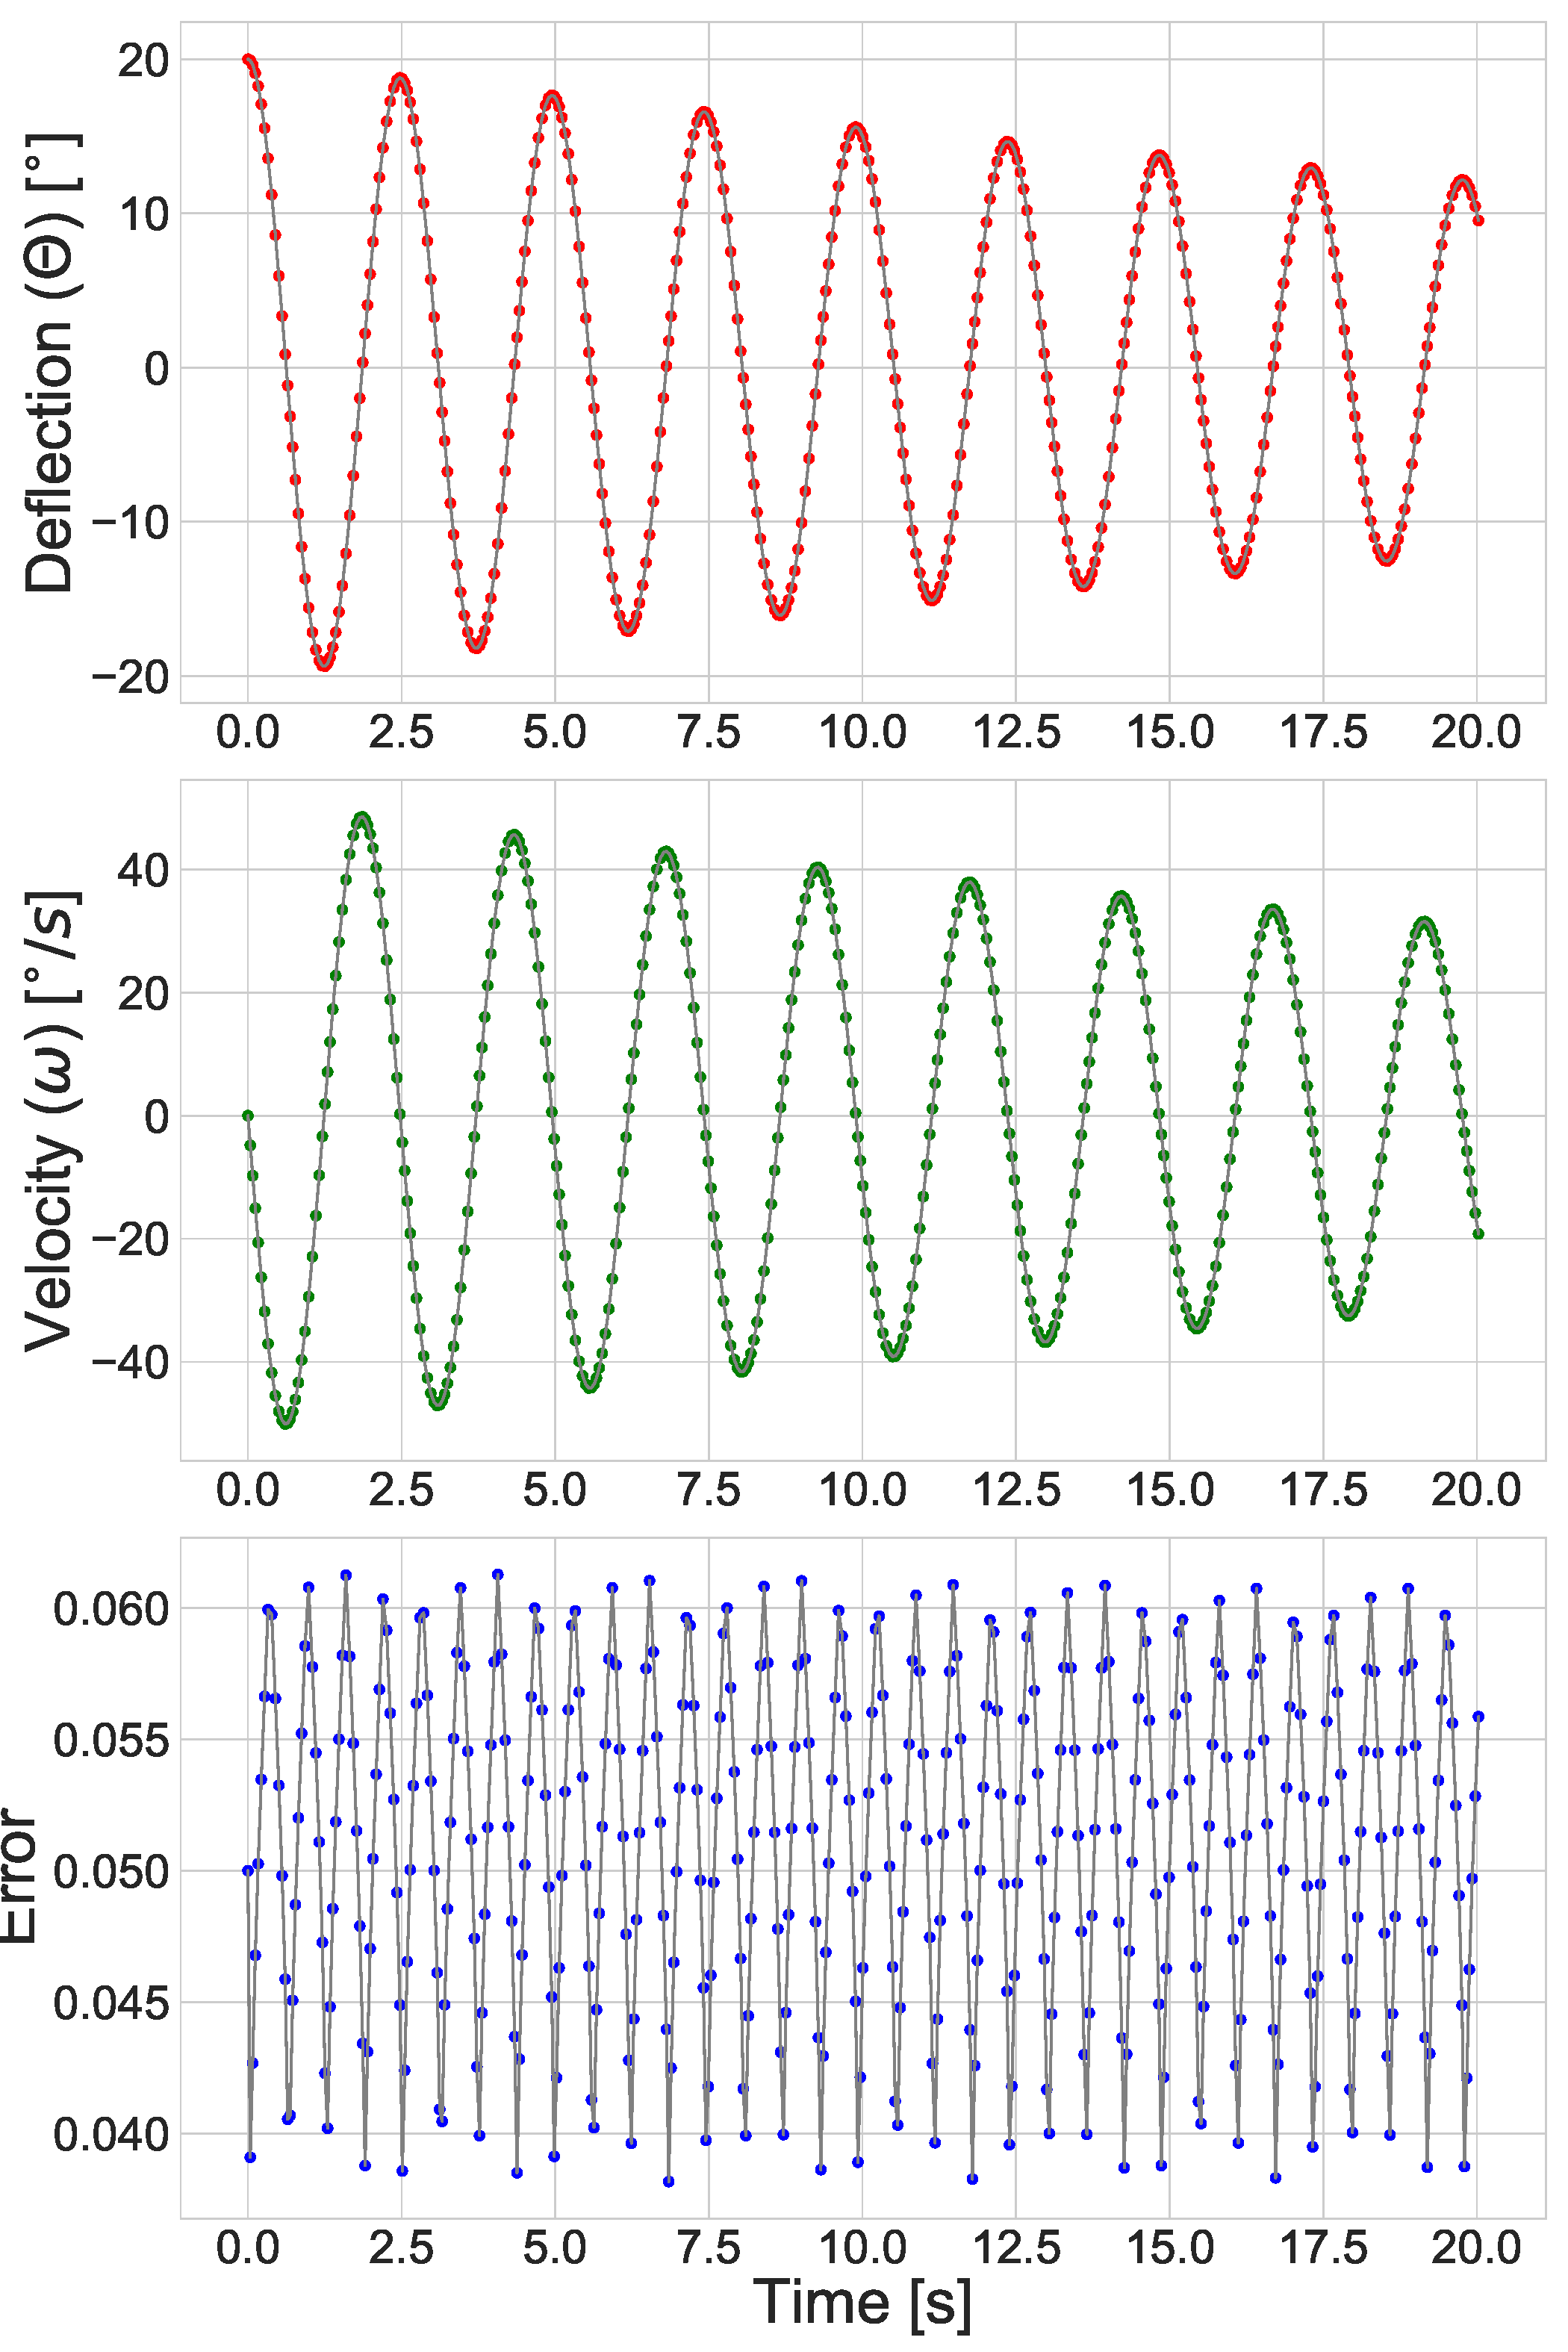
\includegraphics[width=.25\textwidth]{images/theta_omega_runge.pdf}}
\captionof{figure}{Runge-Kutta\\Mat.}\label{fig:4}
\hfill
{\centering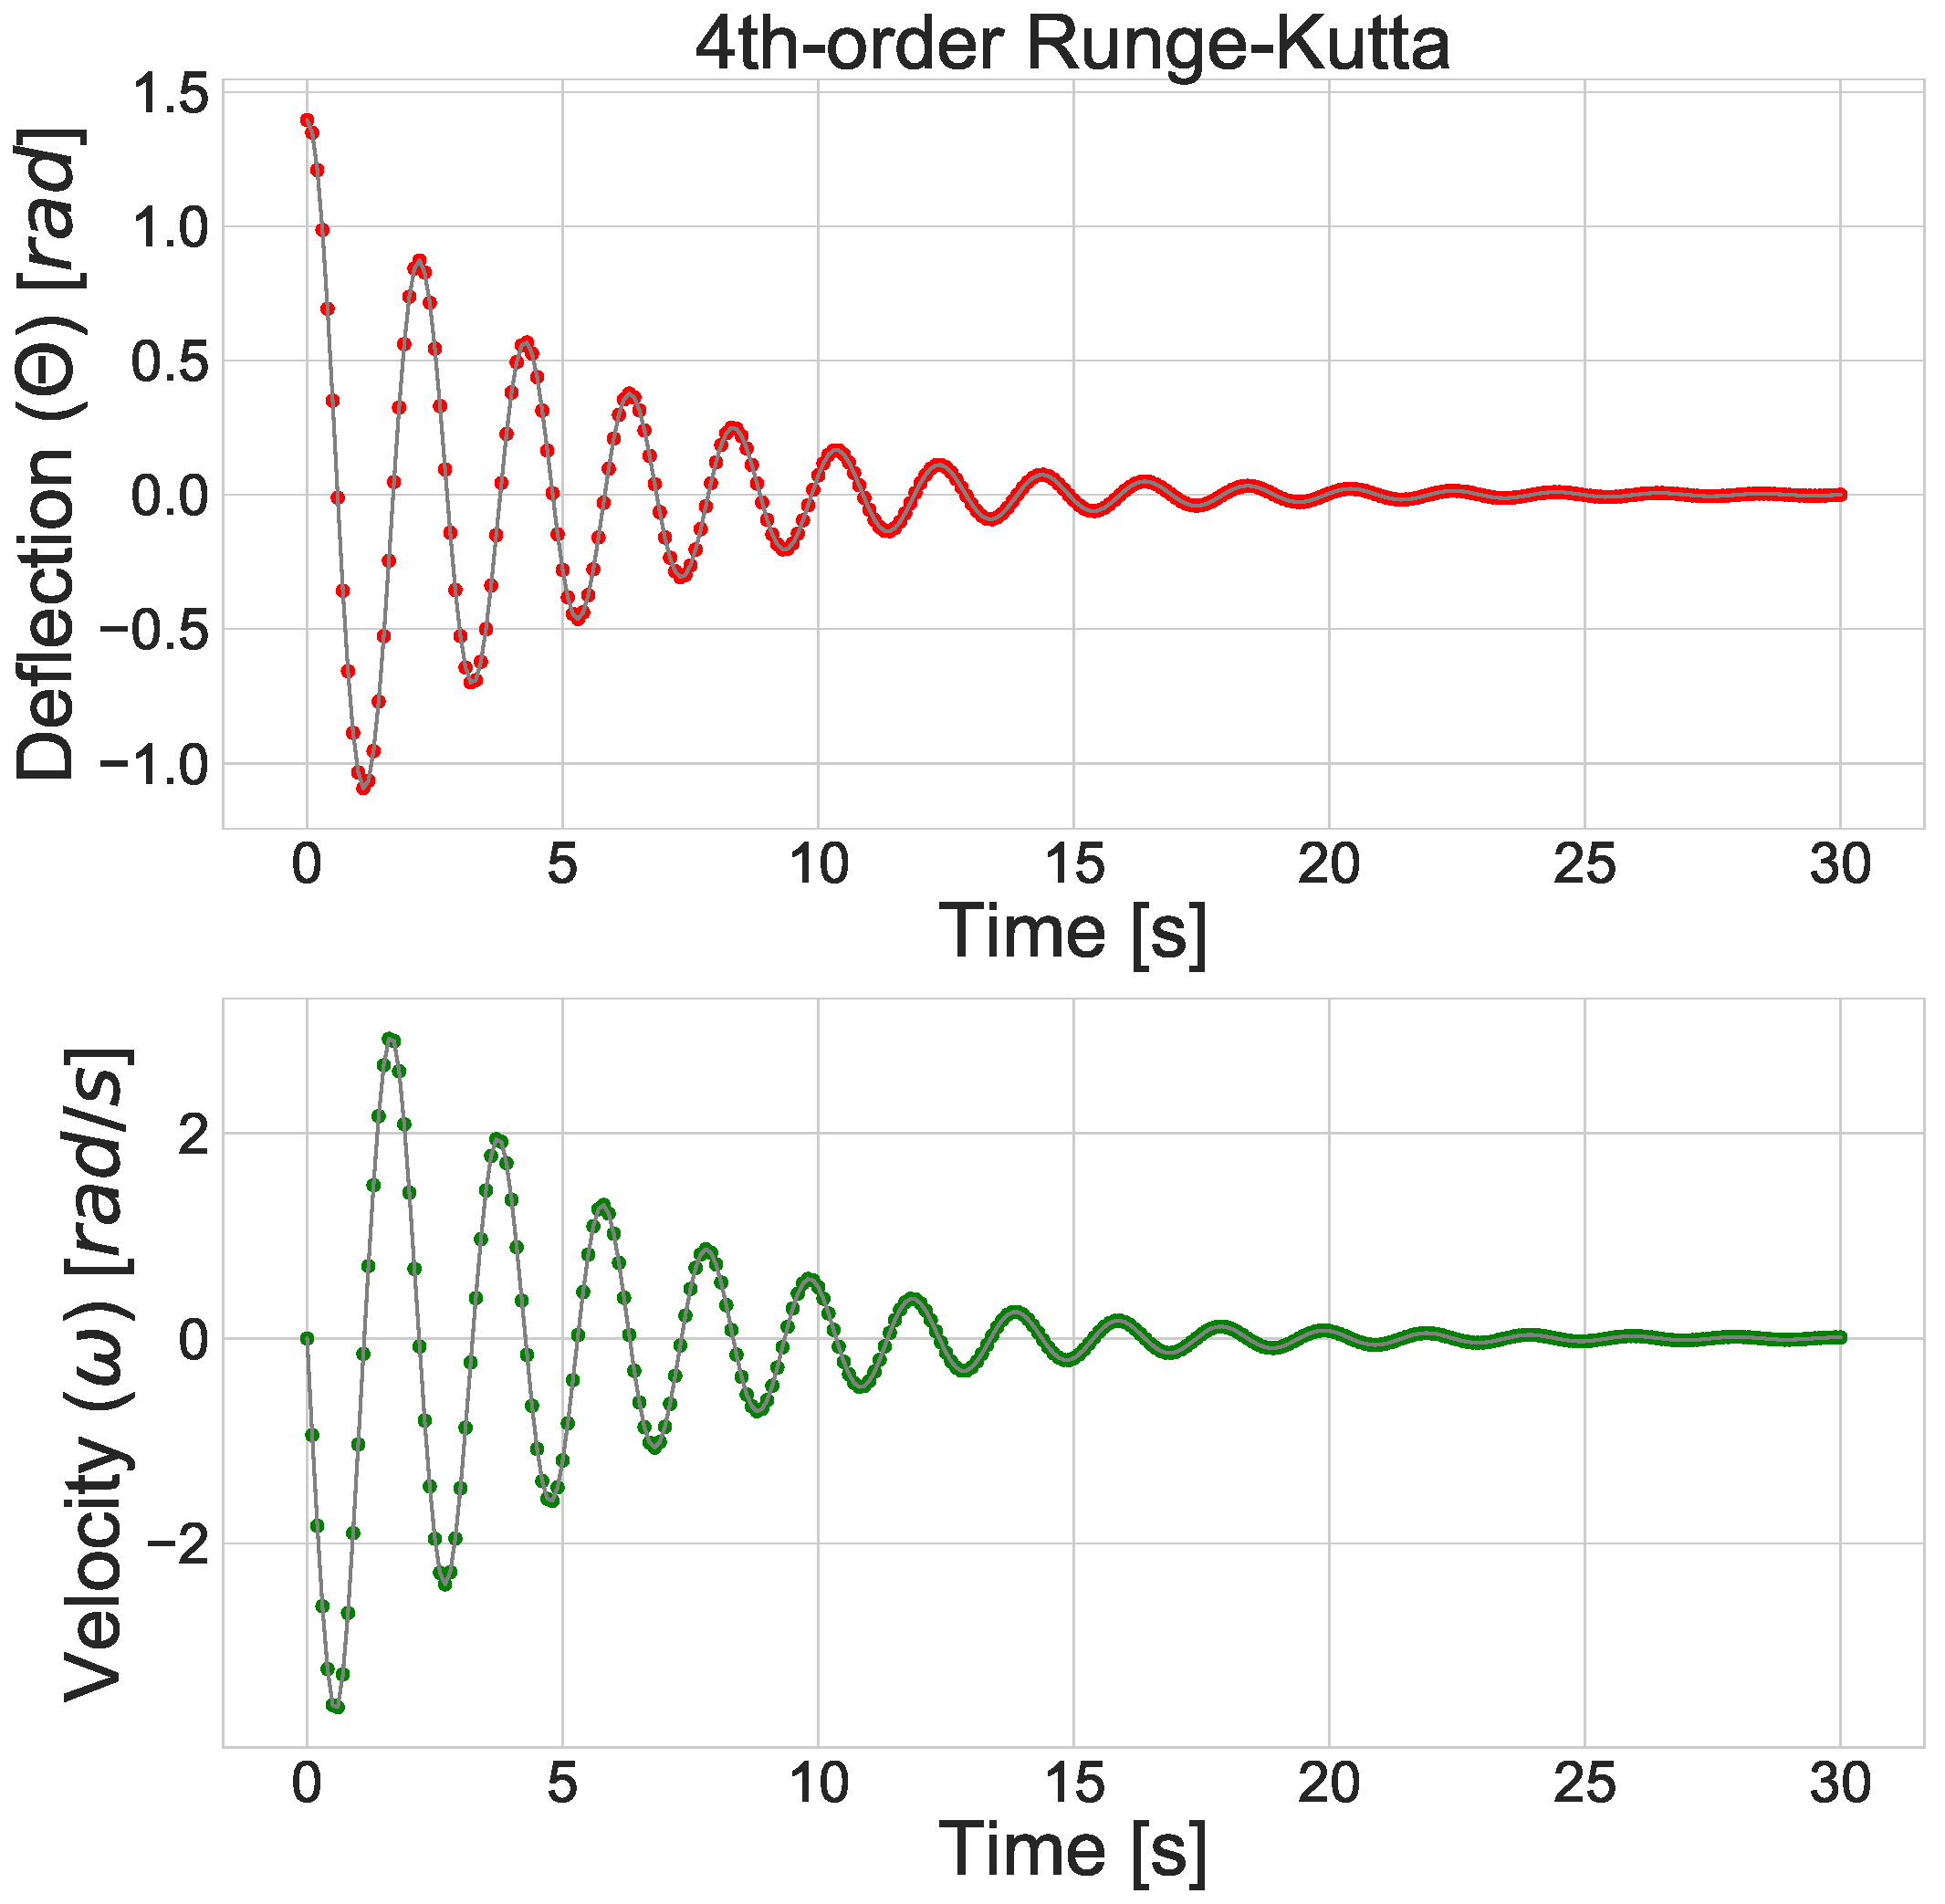
\includegraphics[width=.25\textwidth]{images/theta_omega_runge_damped.pdf}}
\captionof{figure}{Runge-Kutta\\Damp.}\label{fig:5}
\hfill
{\centering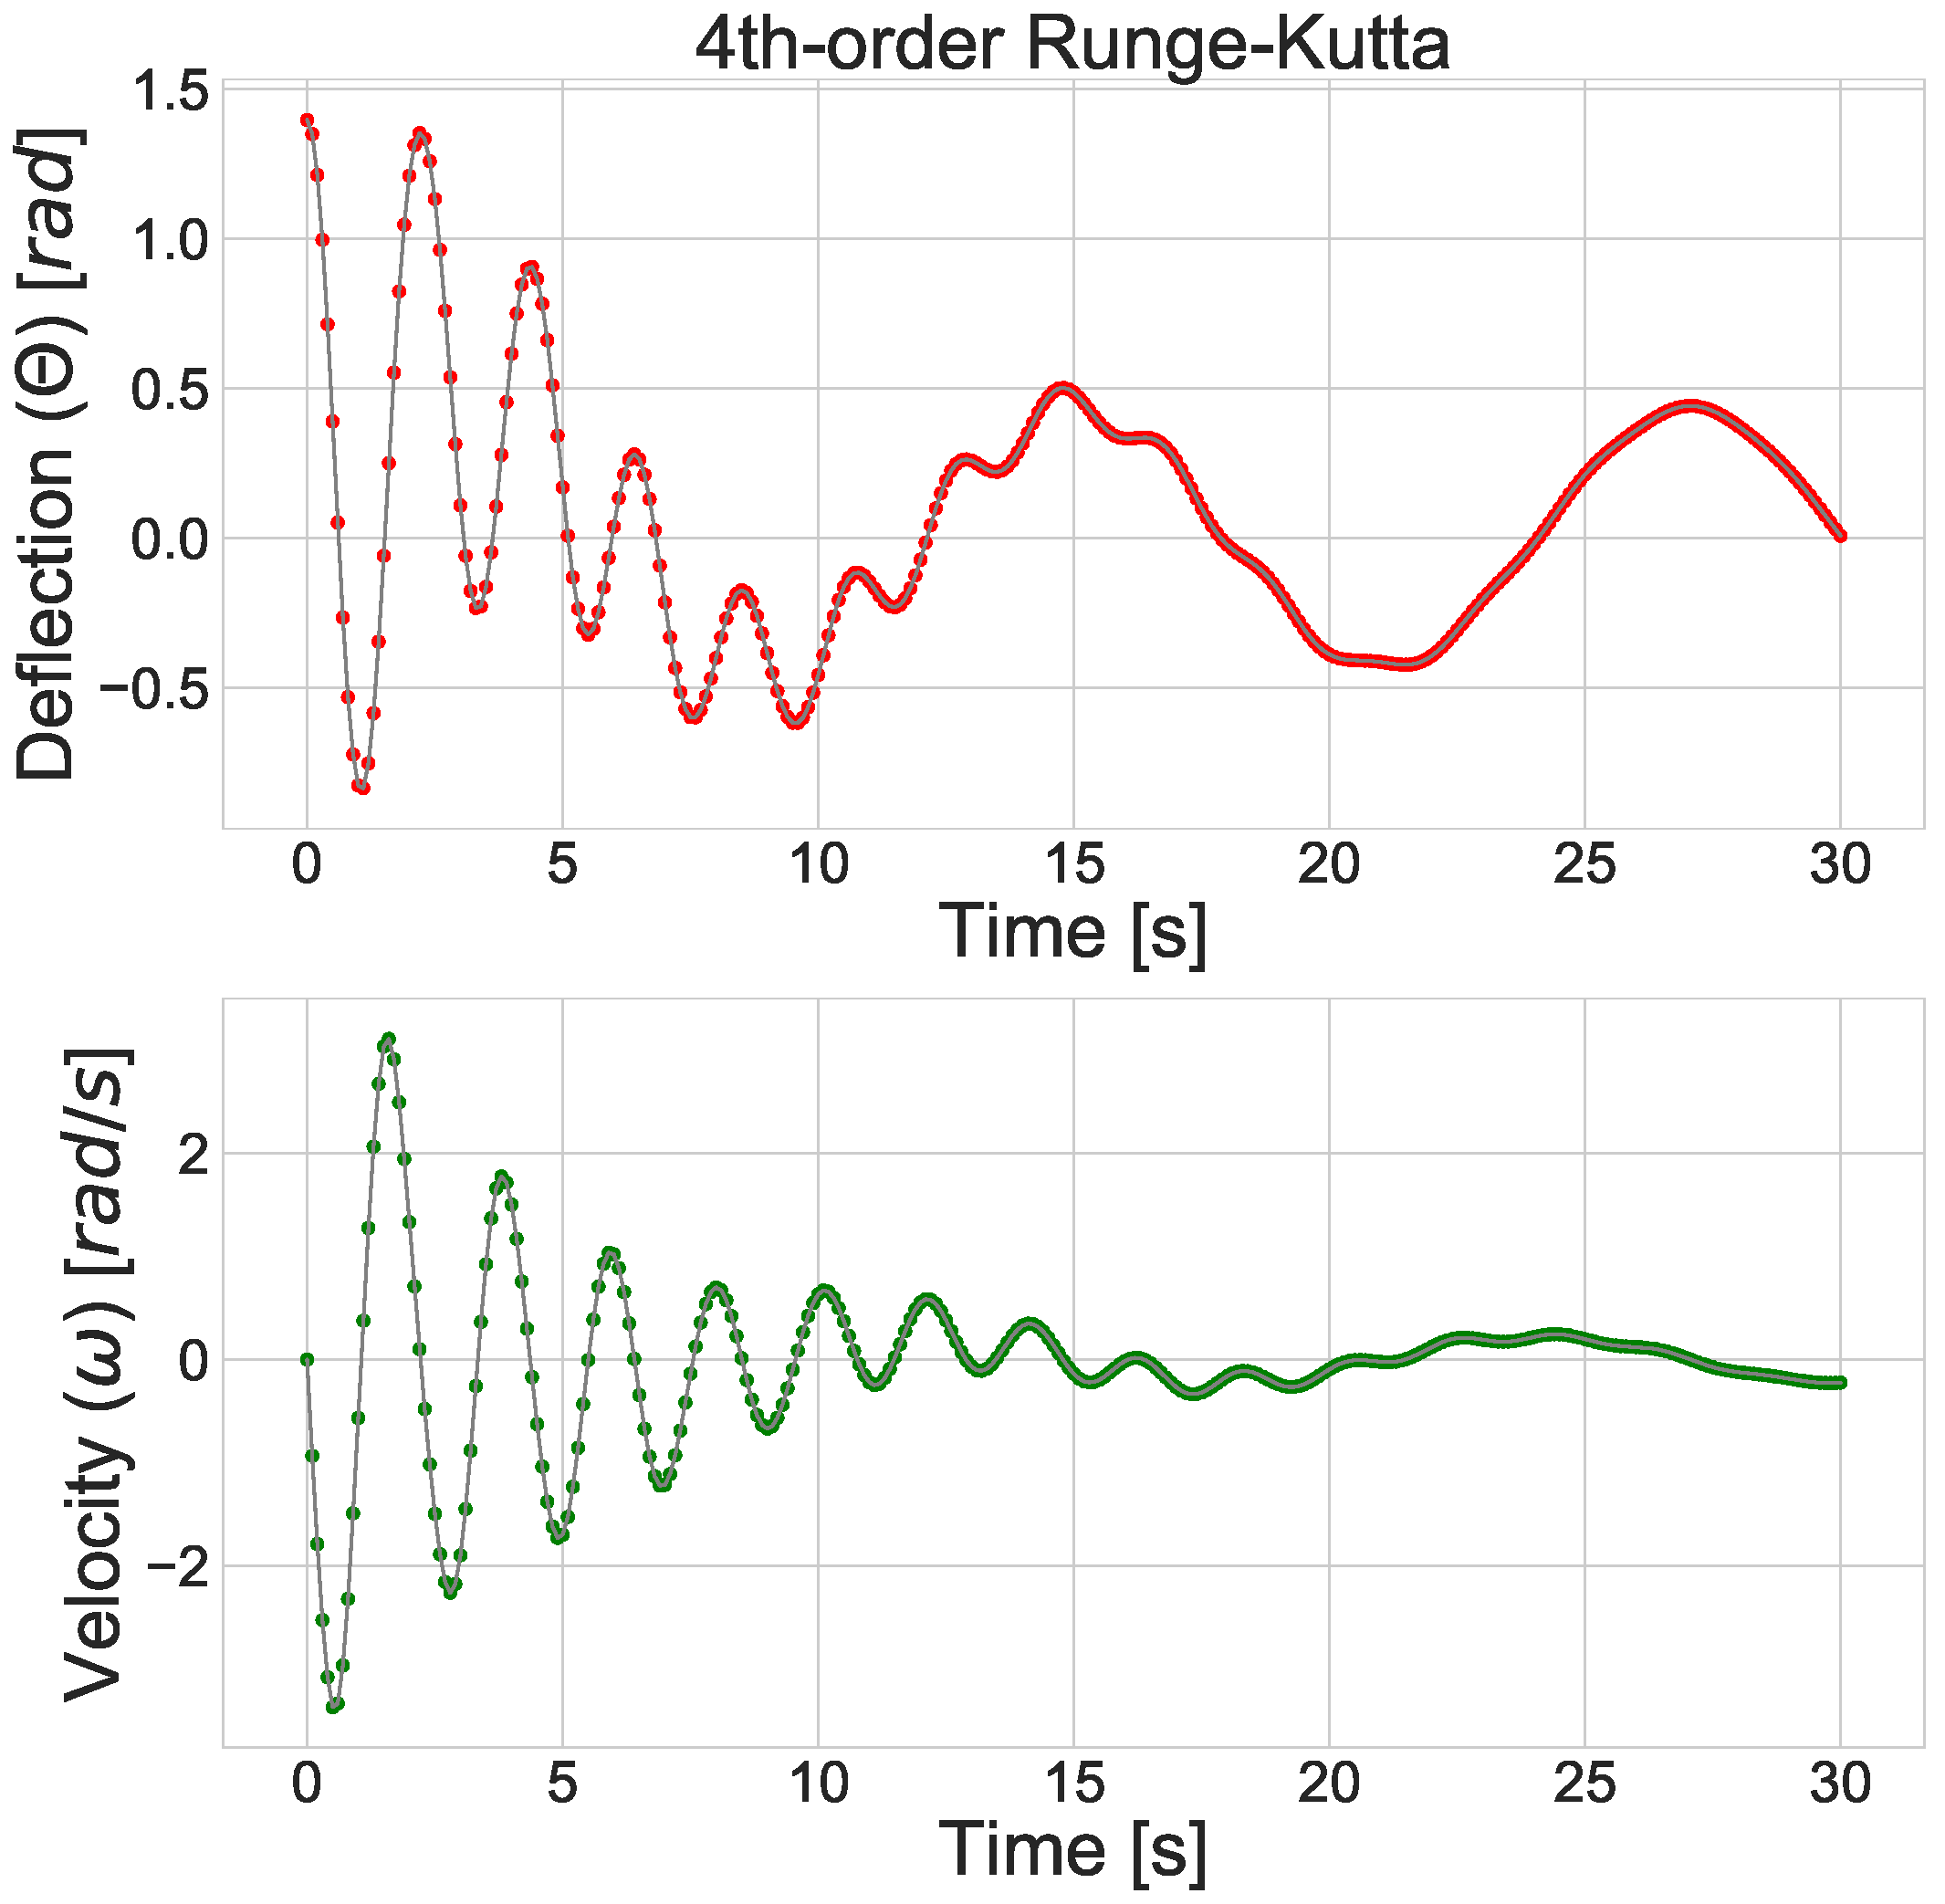
\includegraphics[width=.25\textwidth]{images/theta_omega_runge_dampeddriven.pdf}}
\captionof{figure}{Runge-Kutta\\Damp.-Driv.}\label{fig:6}
\hfill
{\centering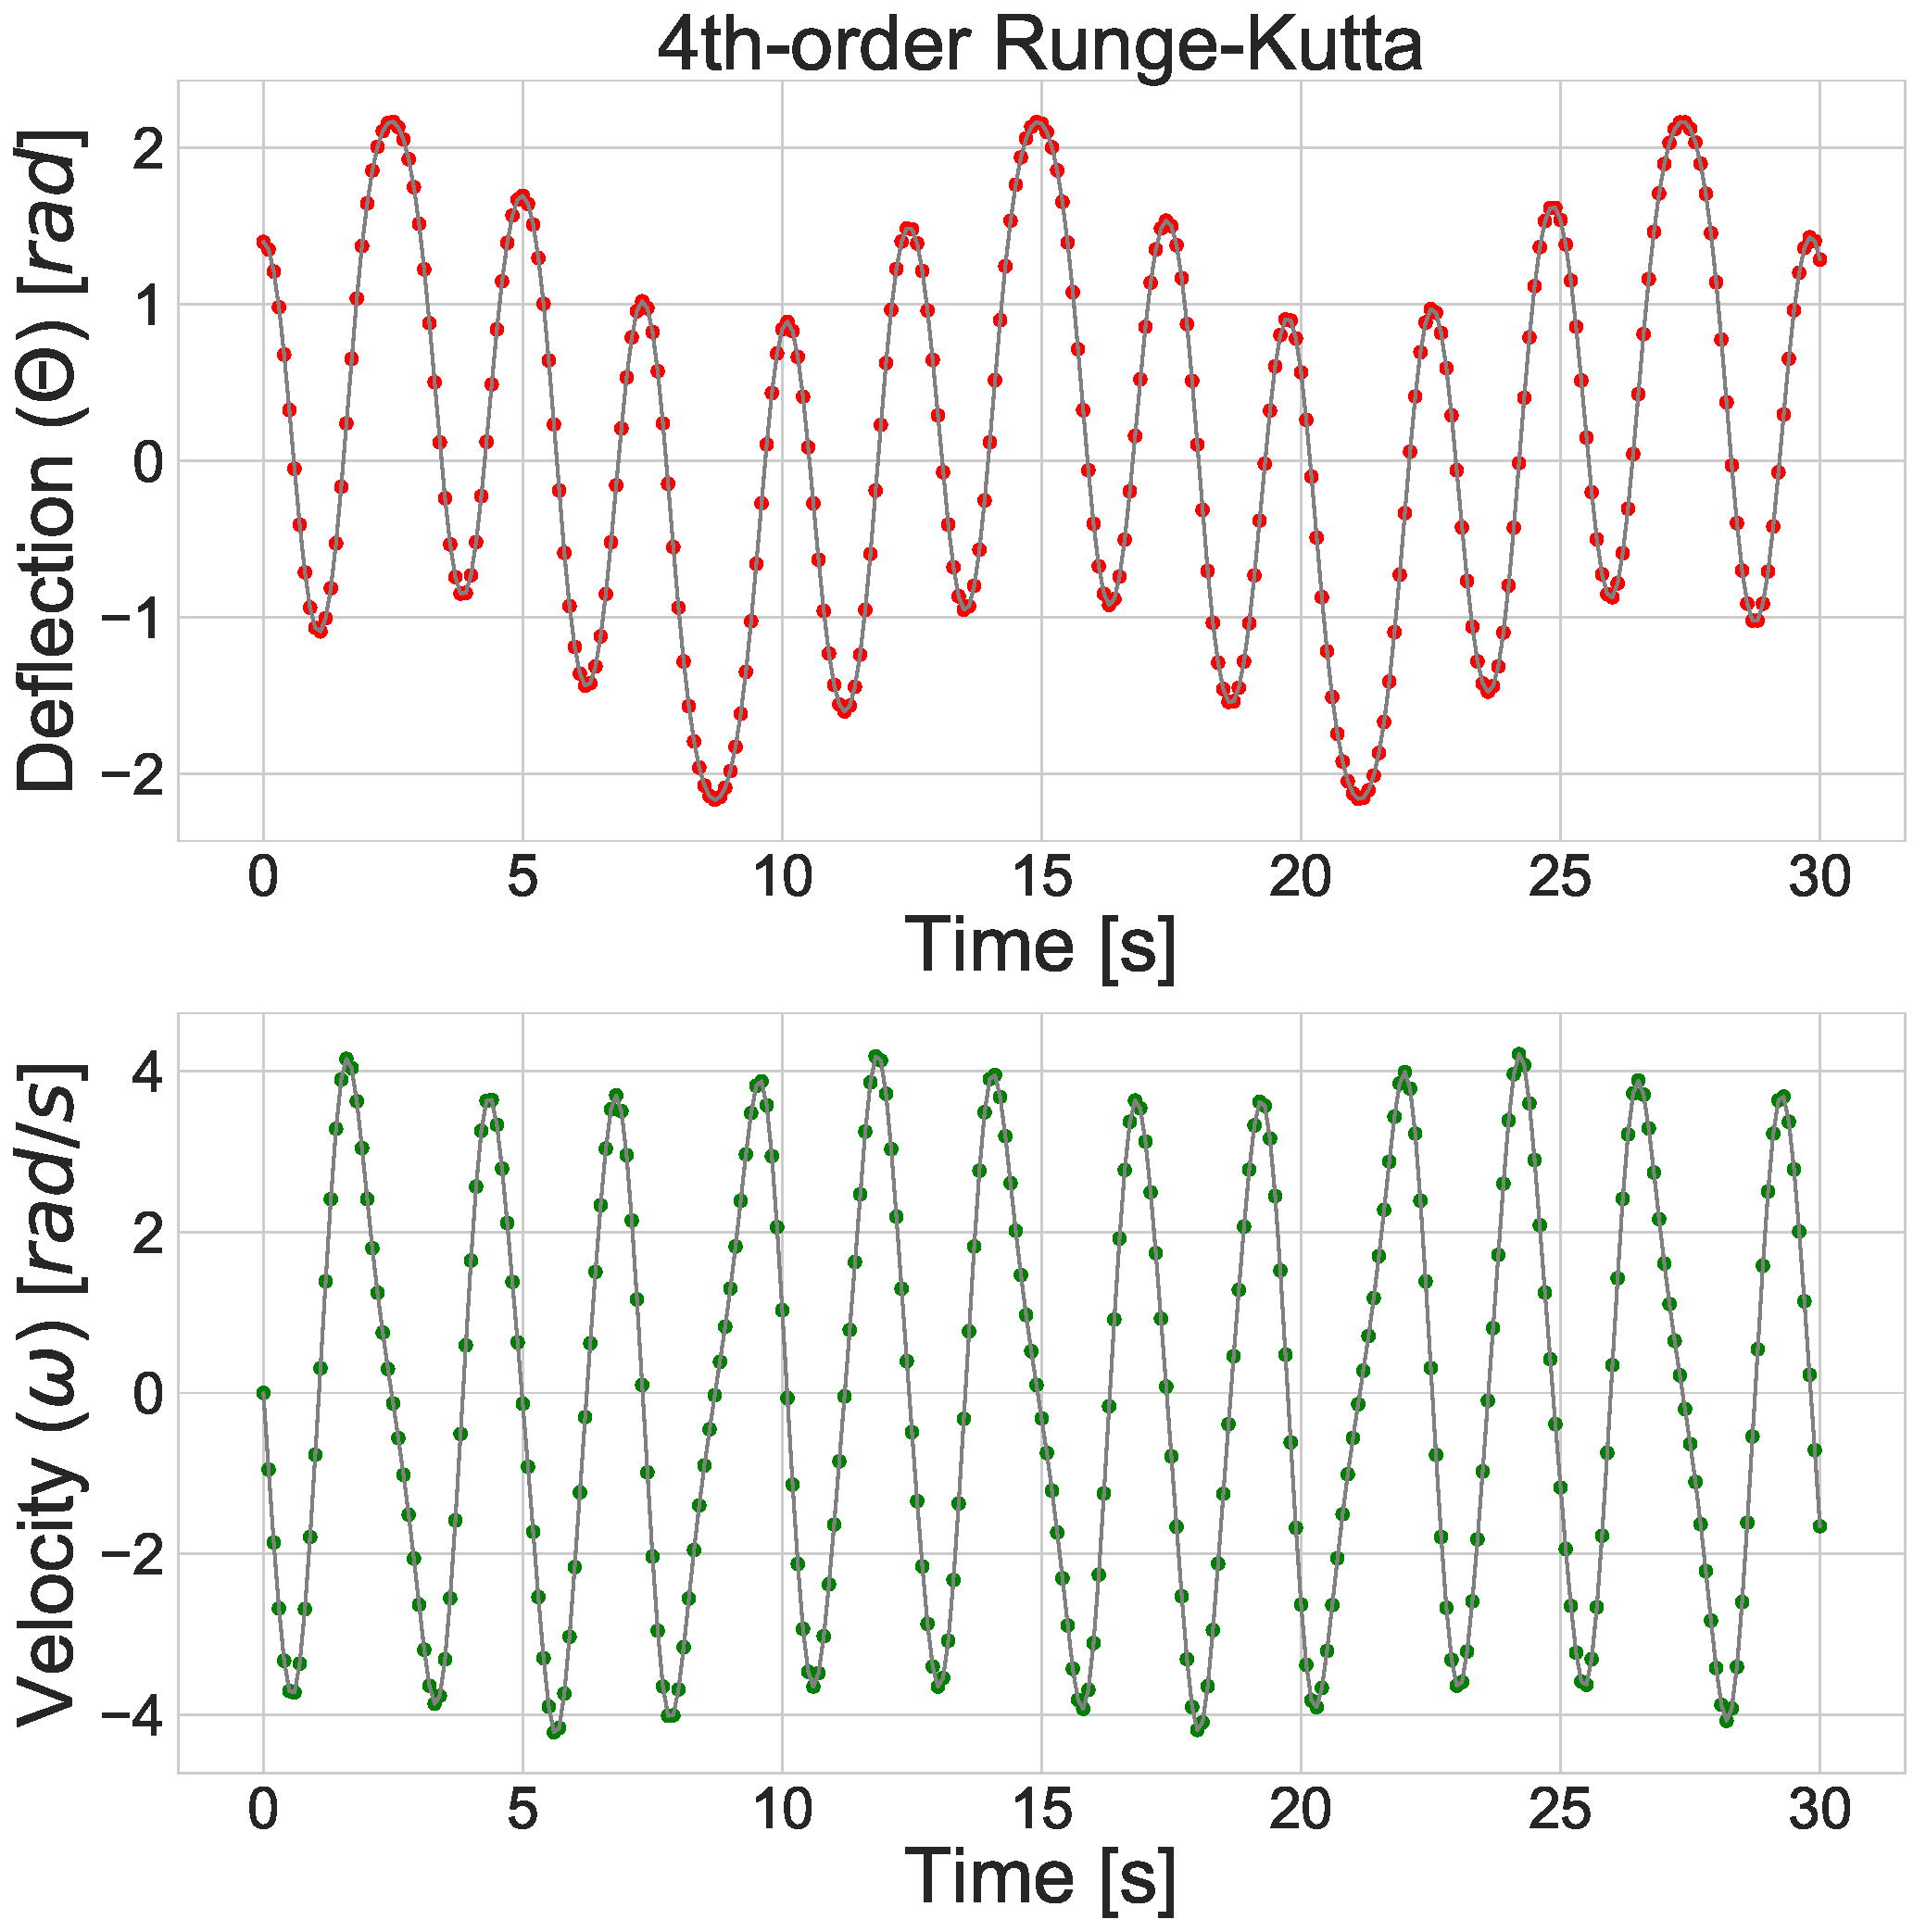
\includegraphics[width=.25\textwidth]{images/theta_omega_runge_driven.pdf}}
\captionof{figure}{Runge-Kutta\\Driv.}\label{fig:7}
\hfill

\end{multicols}
\begin{multicols}{4}

{\centering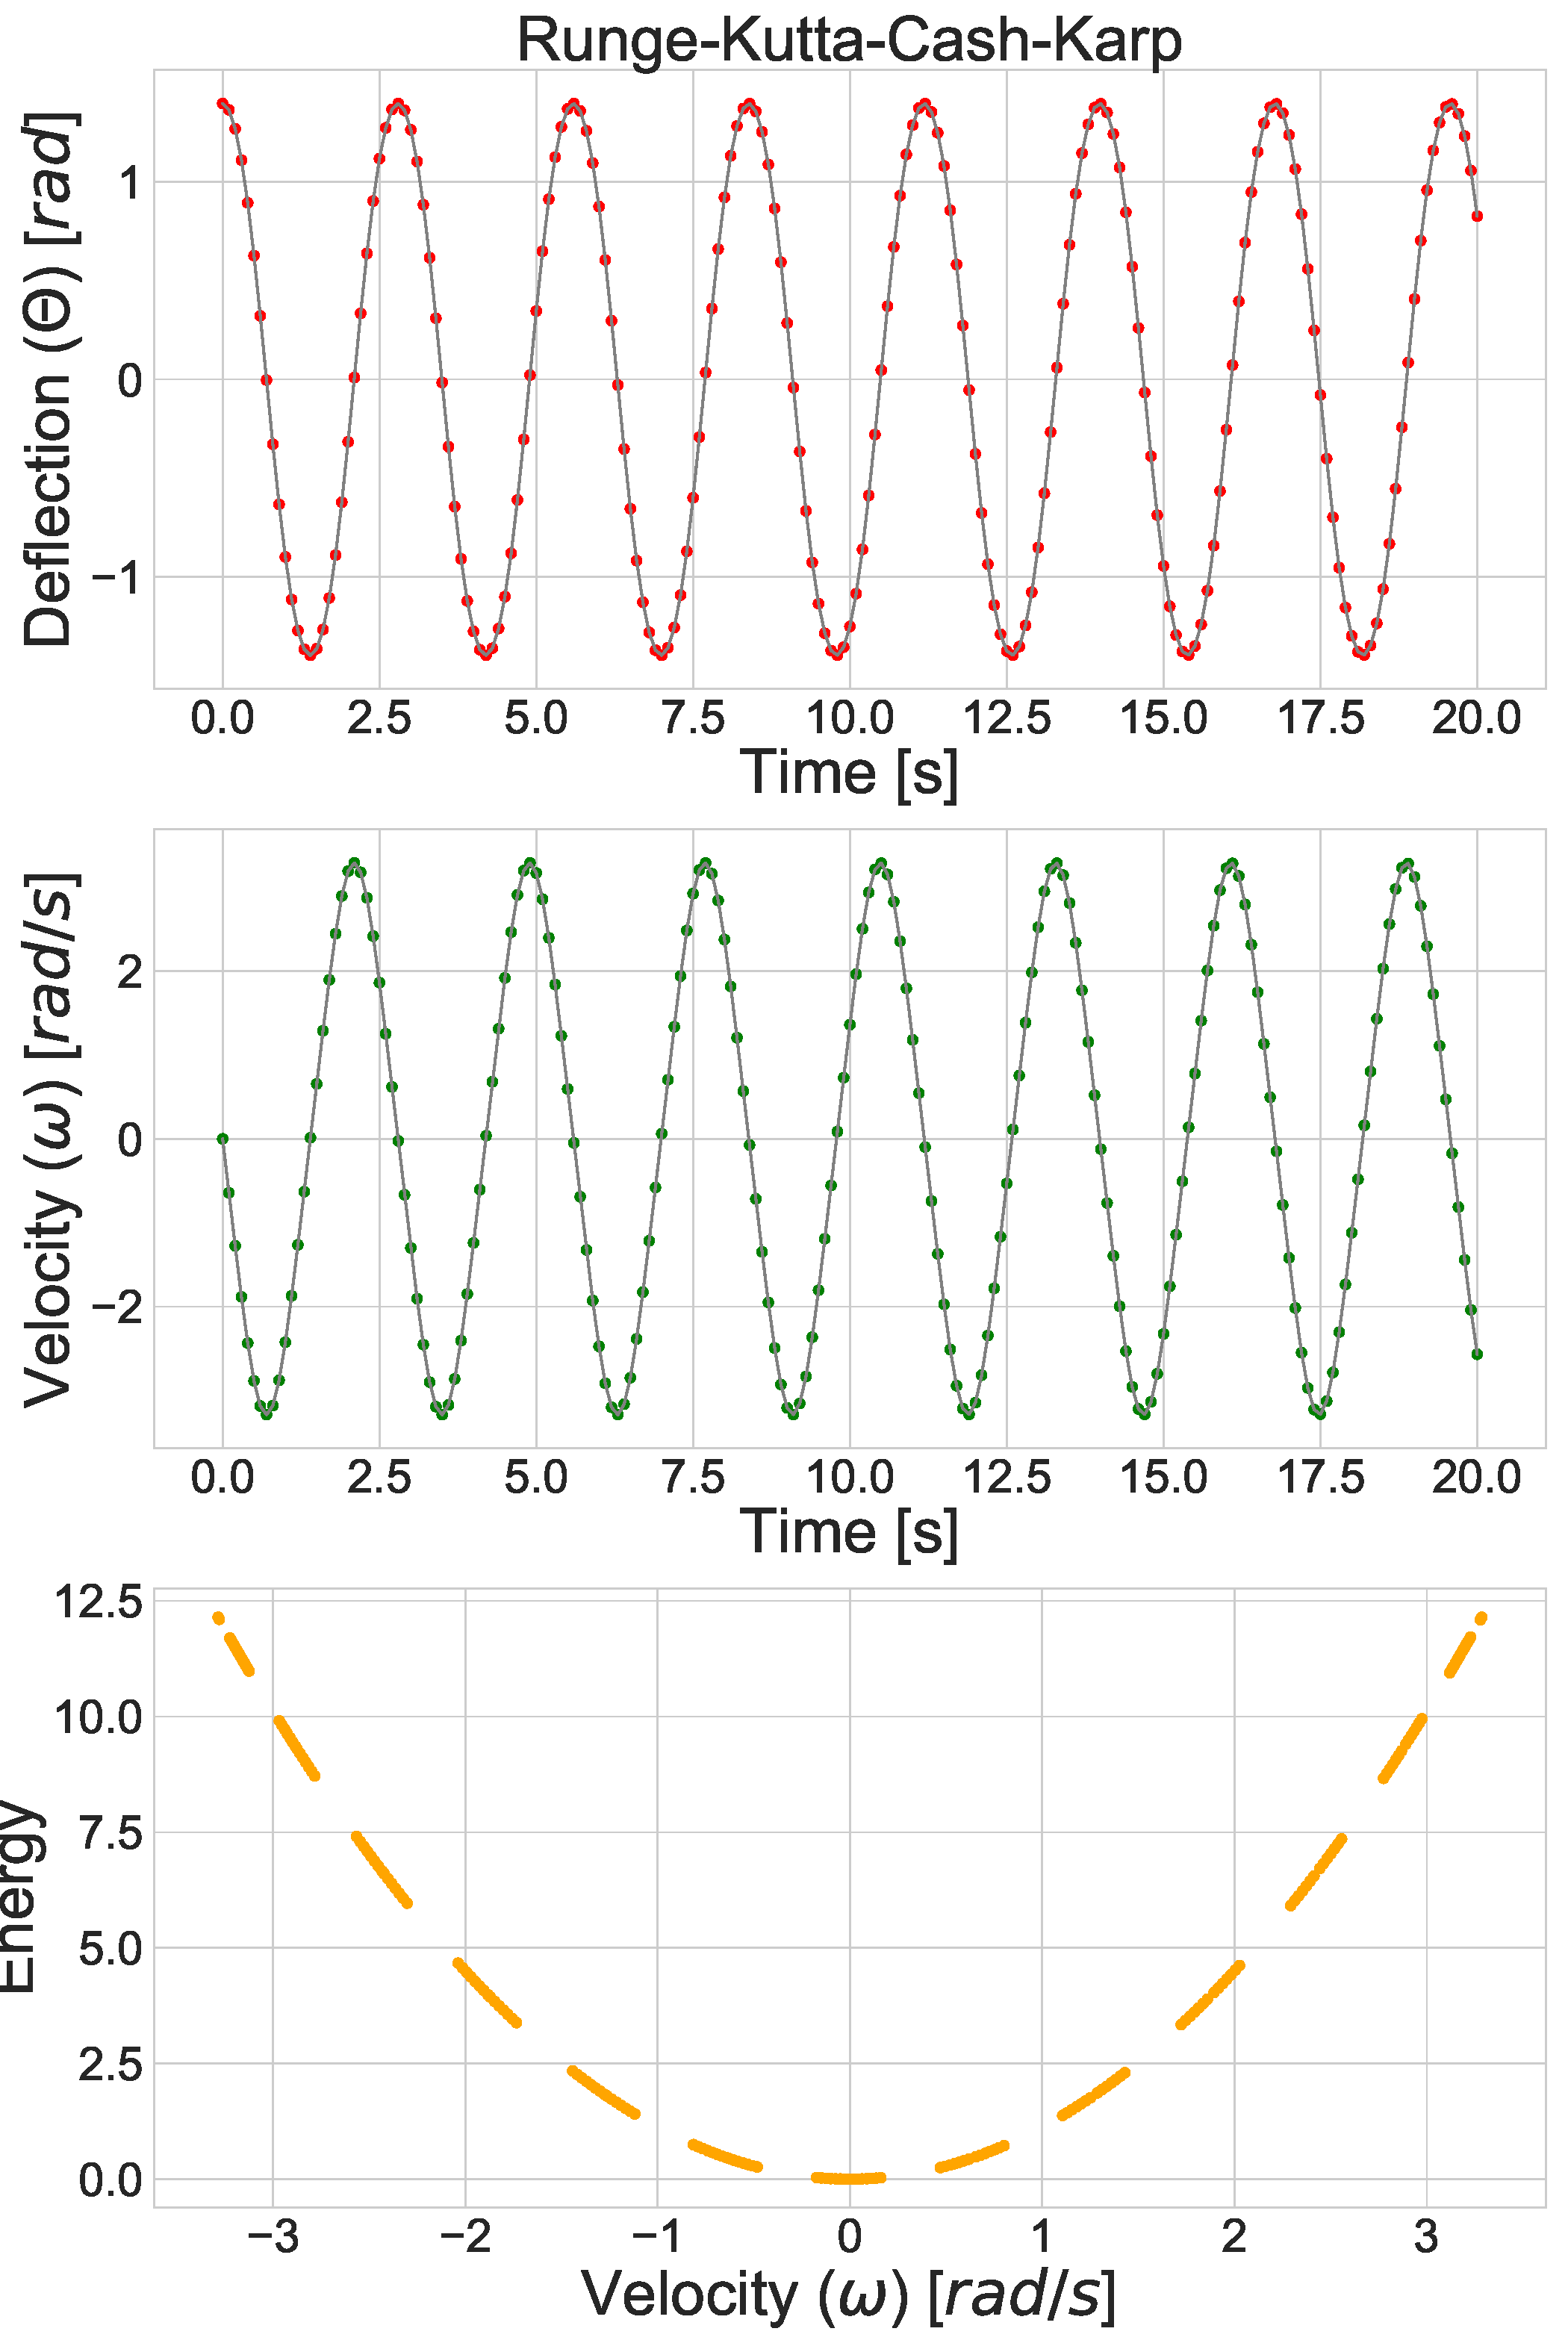
\includegraphics[width=.25\textwidth]{images/theta_omega_rkck.pdf}}
\captionof{figure}{R-K-C-K\\Mat.}\label{fig:8}
\hfill
{\centering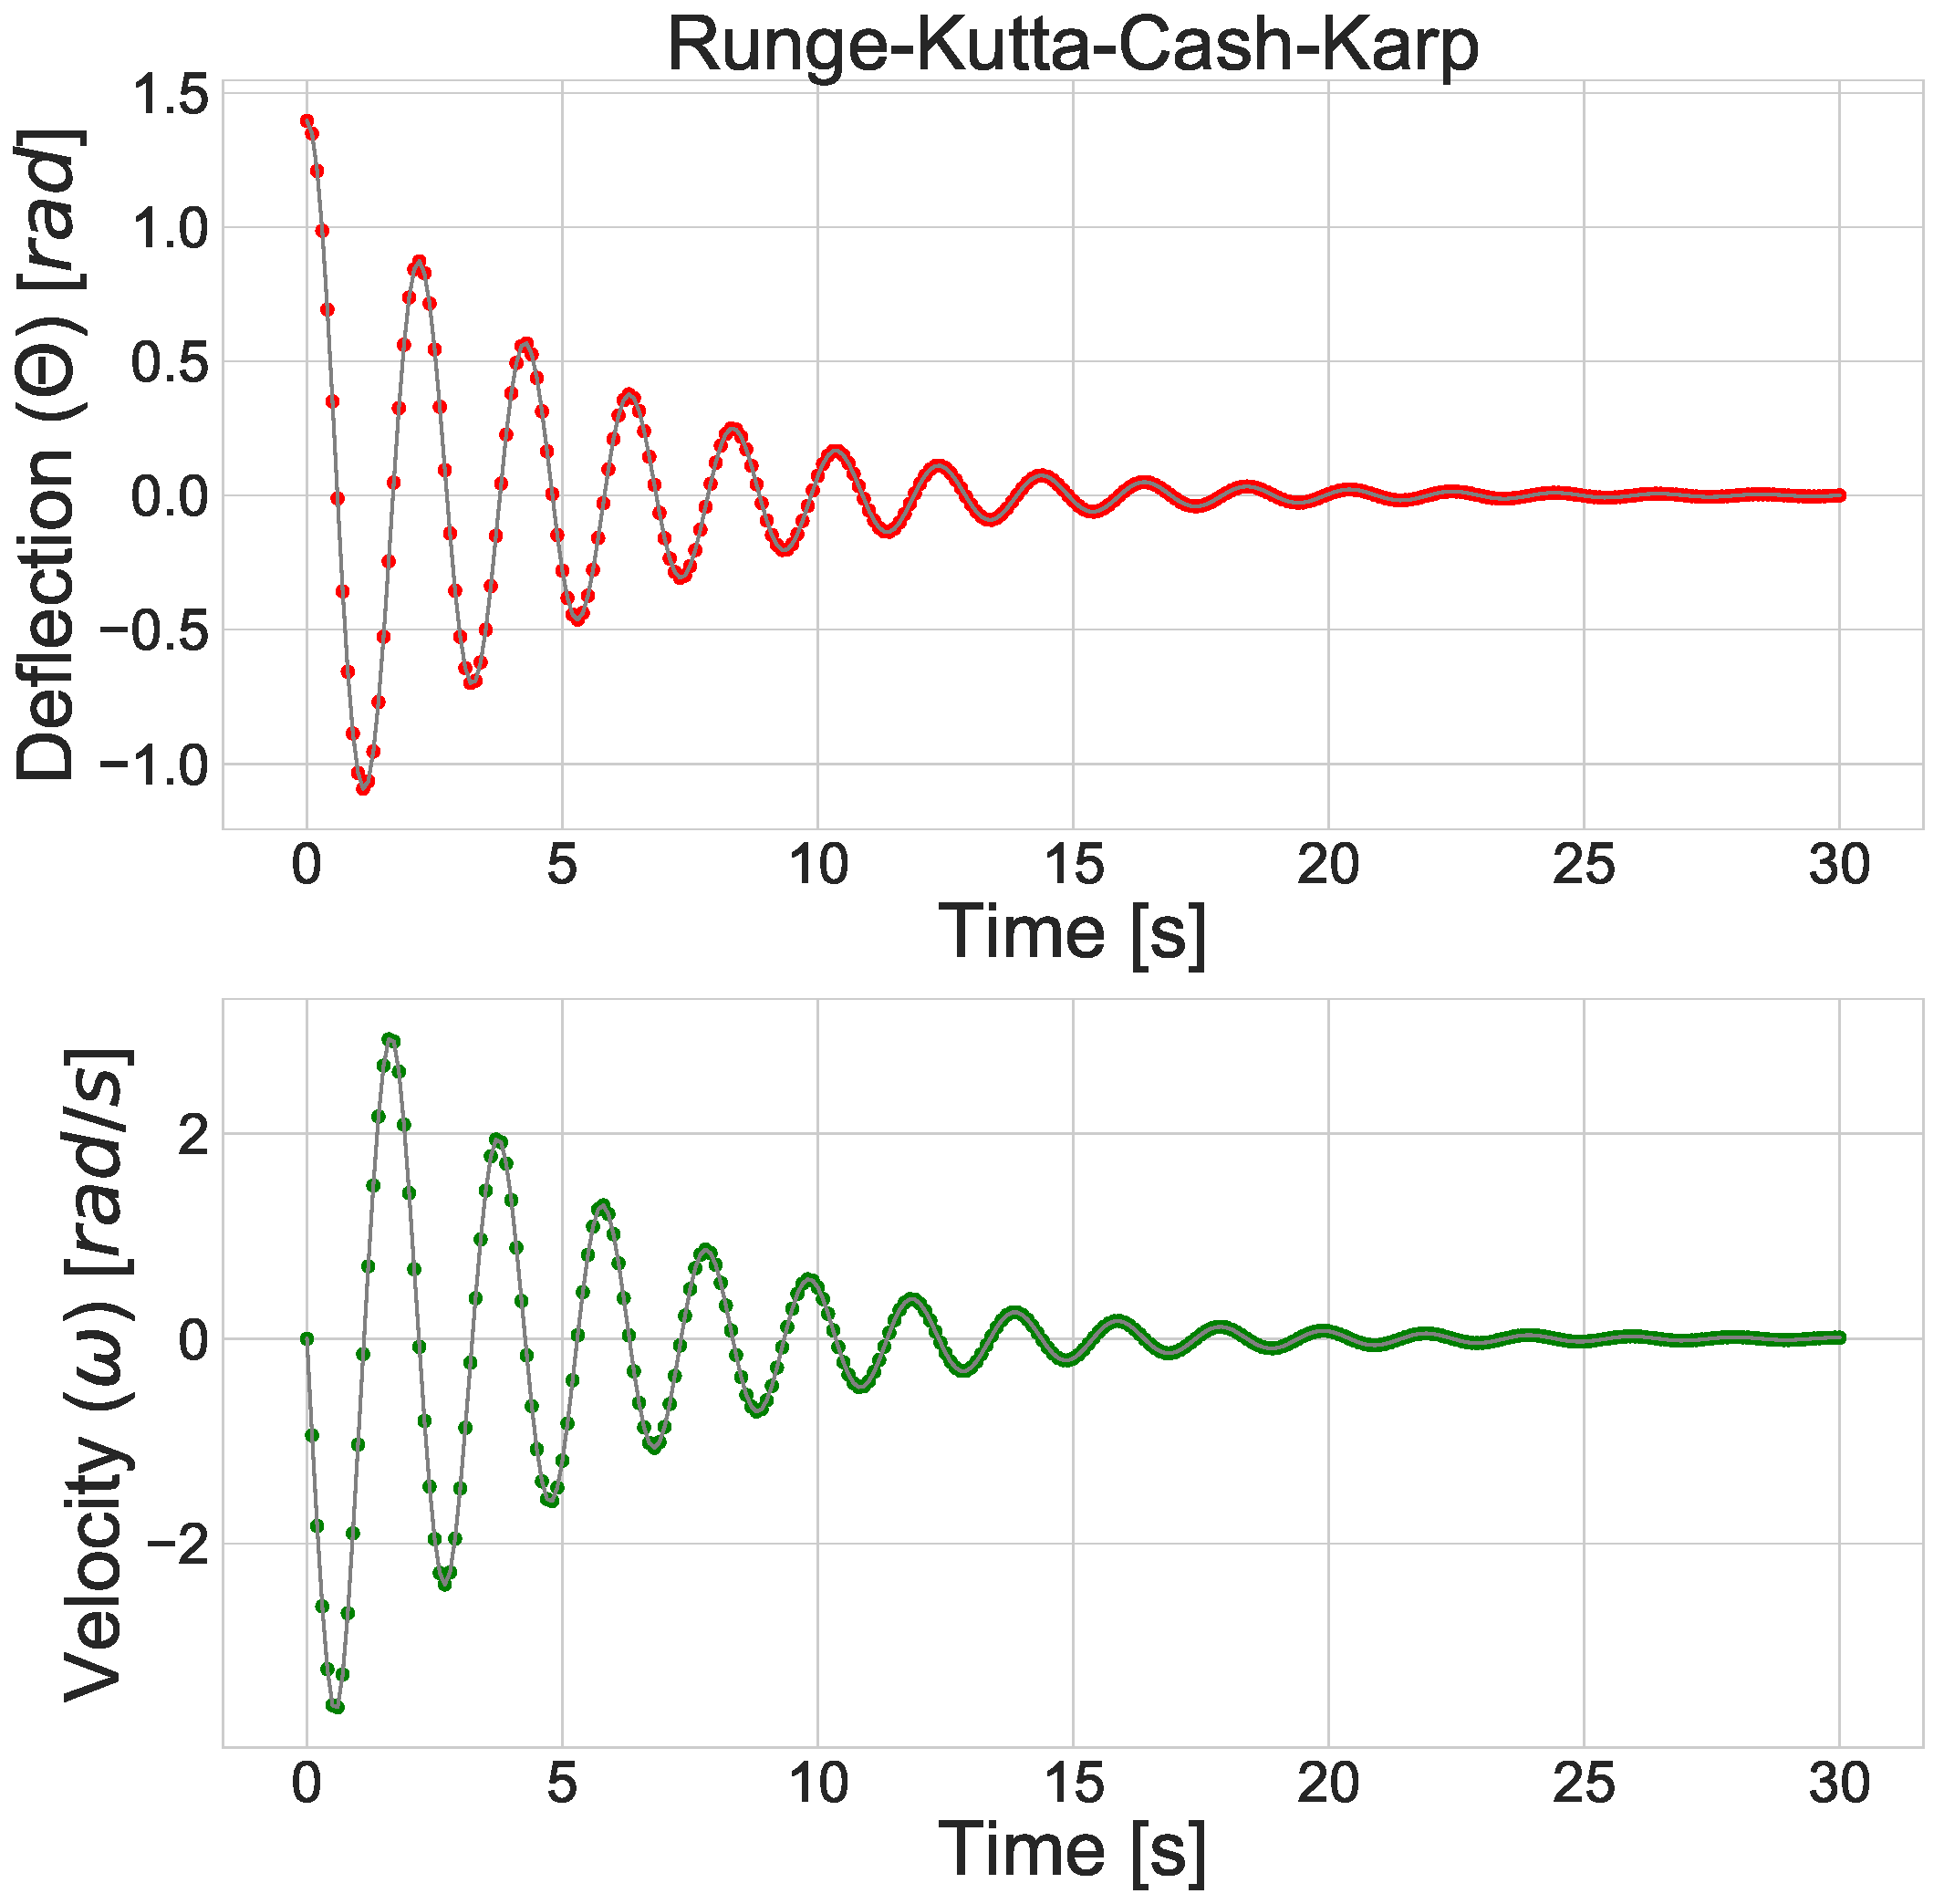
\includegraphics[width=.25\textwidth]{images/theta_omega_rkck_damped.pdf}}
\captionof{figure}{R-K-C-K\\Damp.}\label{fig:9}
\hfill
{\centering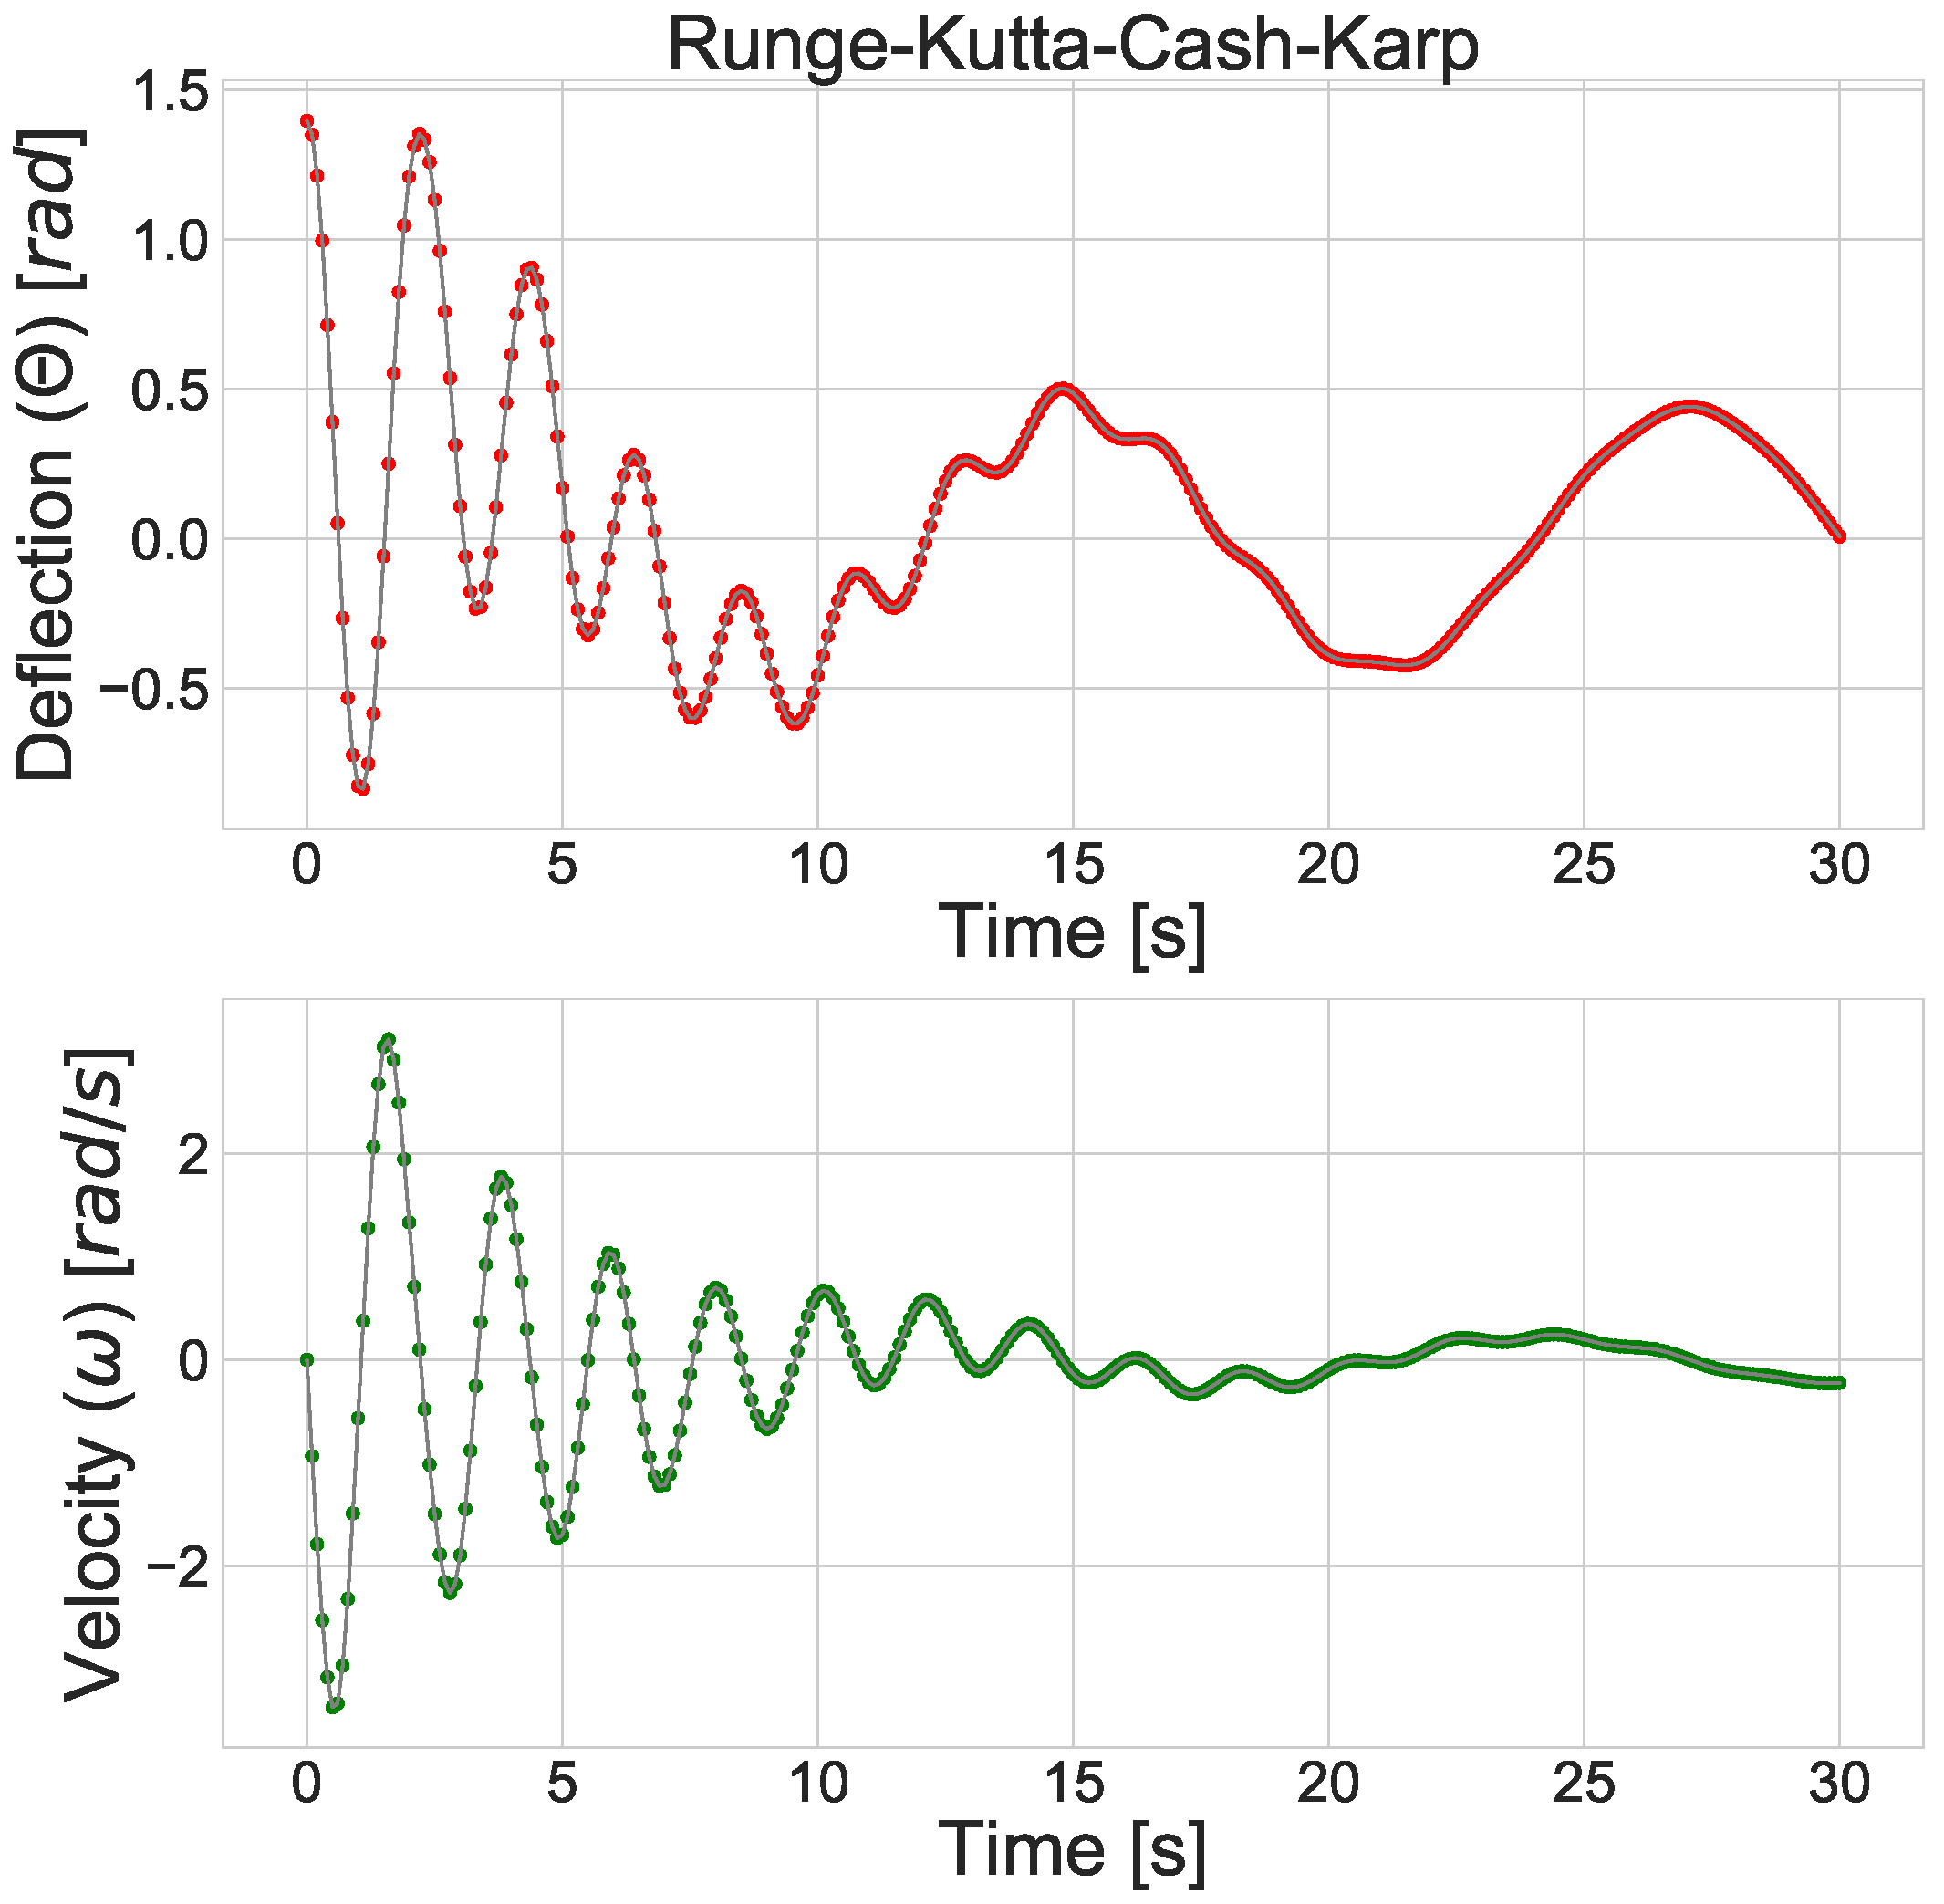
\includegraphics[width=.25\textwidth]{images/theta_omega_rkck_dampeddriven.pdf}}
\captionof{figure}{R-K-C-K\\Damp.-Driv.}\label{fig:10}
\hfill
{\centering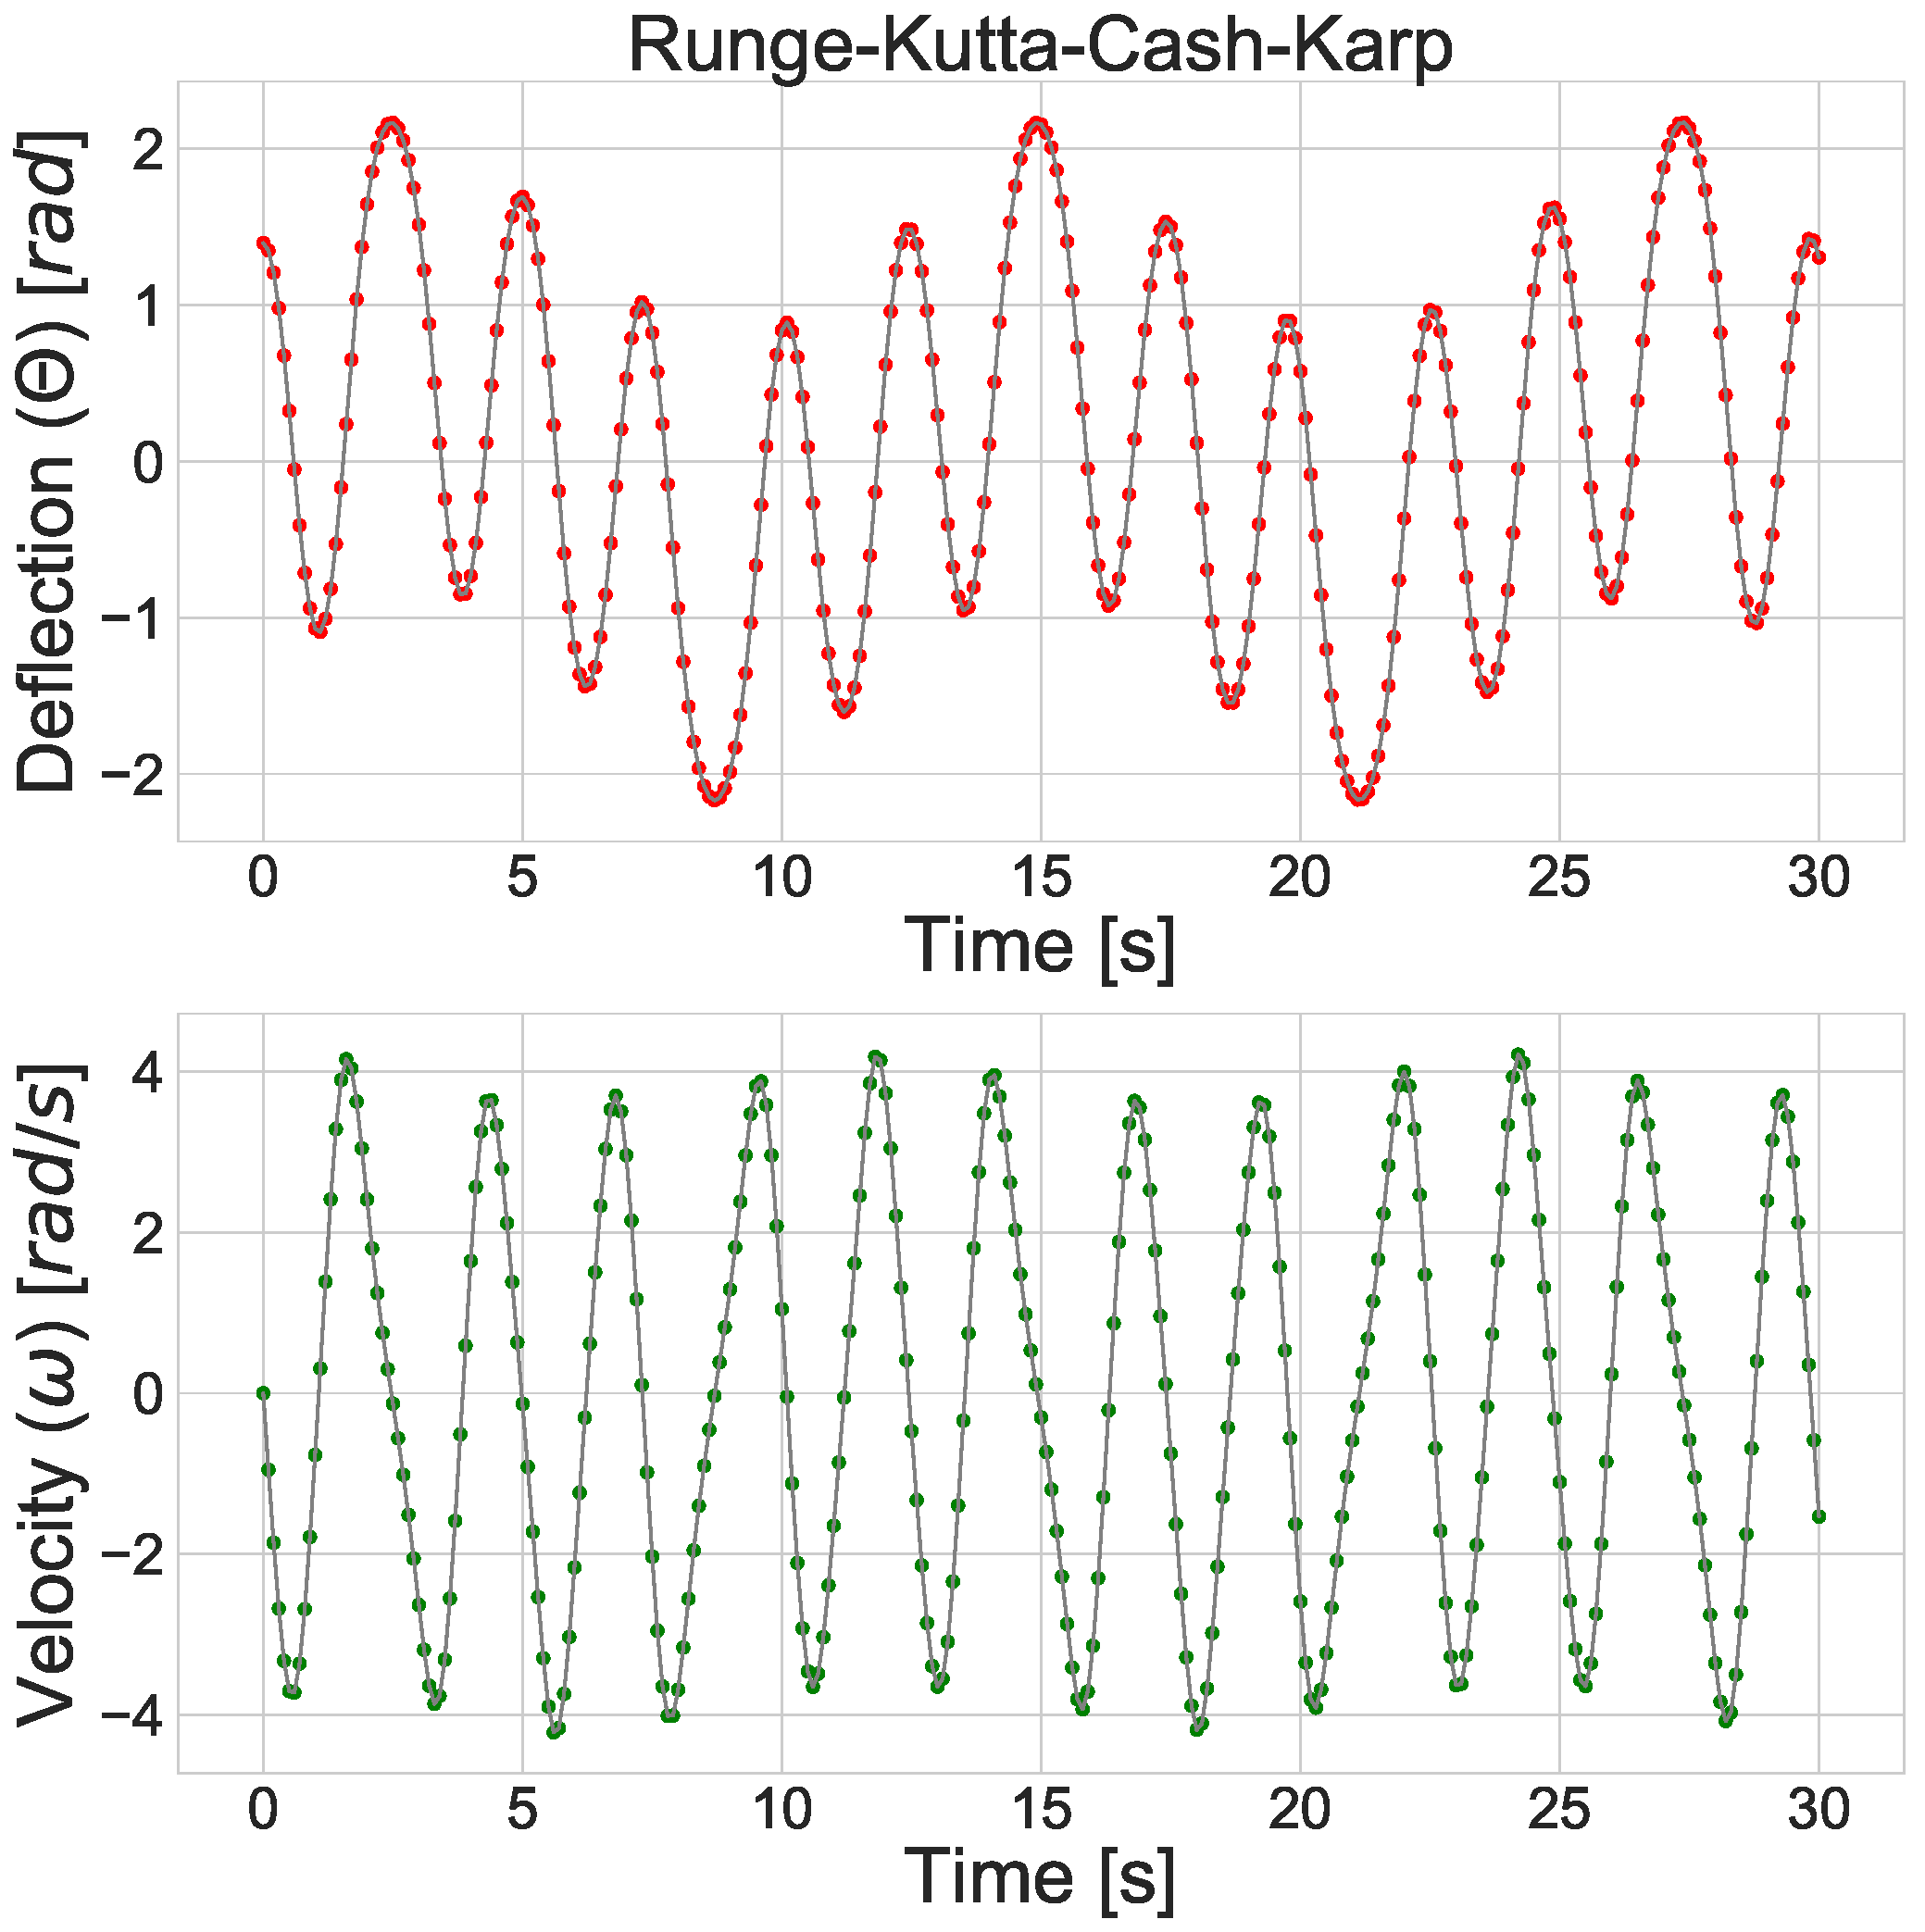
\includegraphics[width=.25\textwidth]{images/theta_omega_rkck_driven.pdf}}
\captionof{figure}{R-K-C-K\\Driv.}\label{fig:11}
\hfill

\end{multicols}
\begin{multicols}{4}

{\centering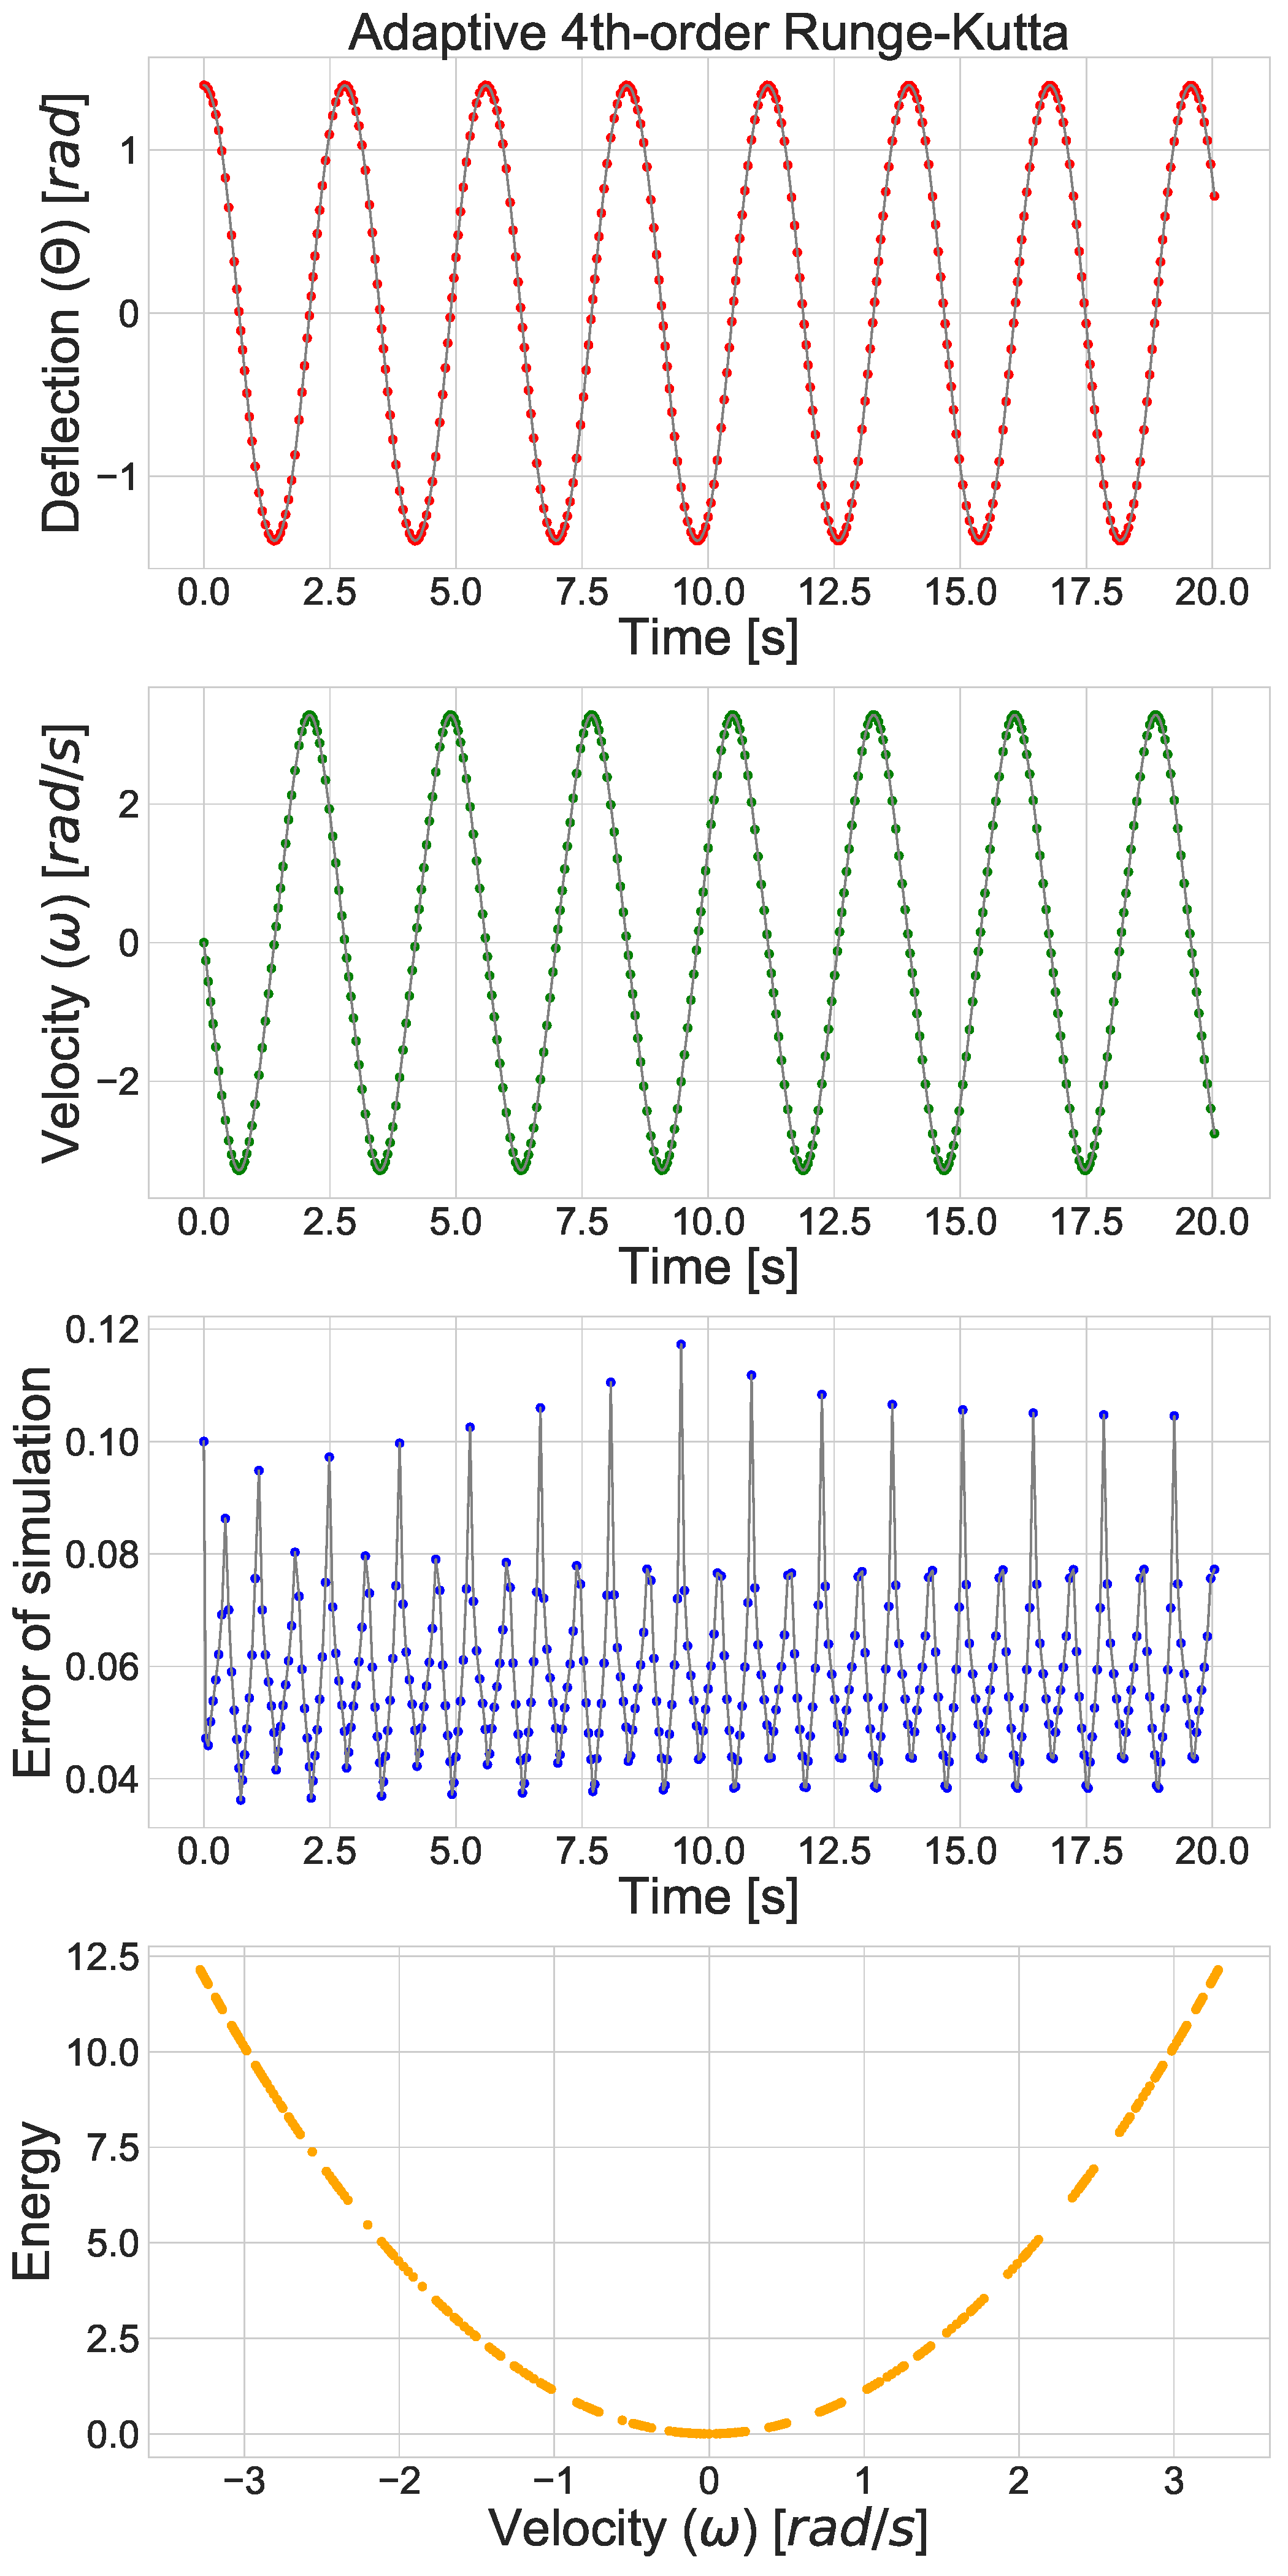
\includegraphics[width=.25\textwidth]{images/theta_omega_adapt_runge.pdf}}
\captionof{figure}{Ad. Runge-Kutta\\Mat.}\label{fig:12}
\hfill
{\centering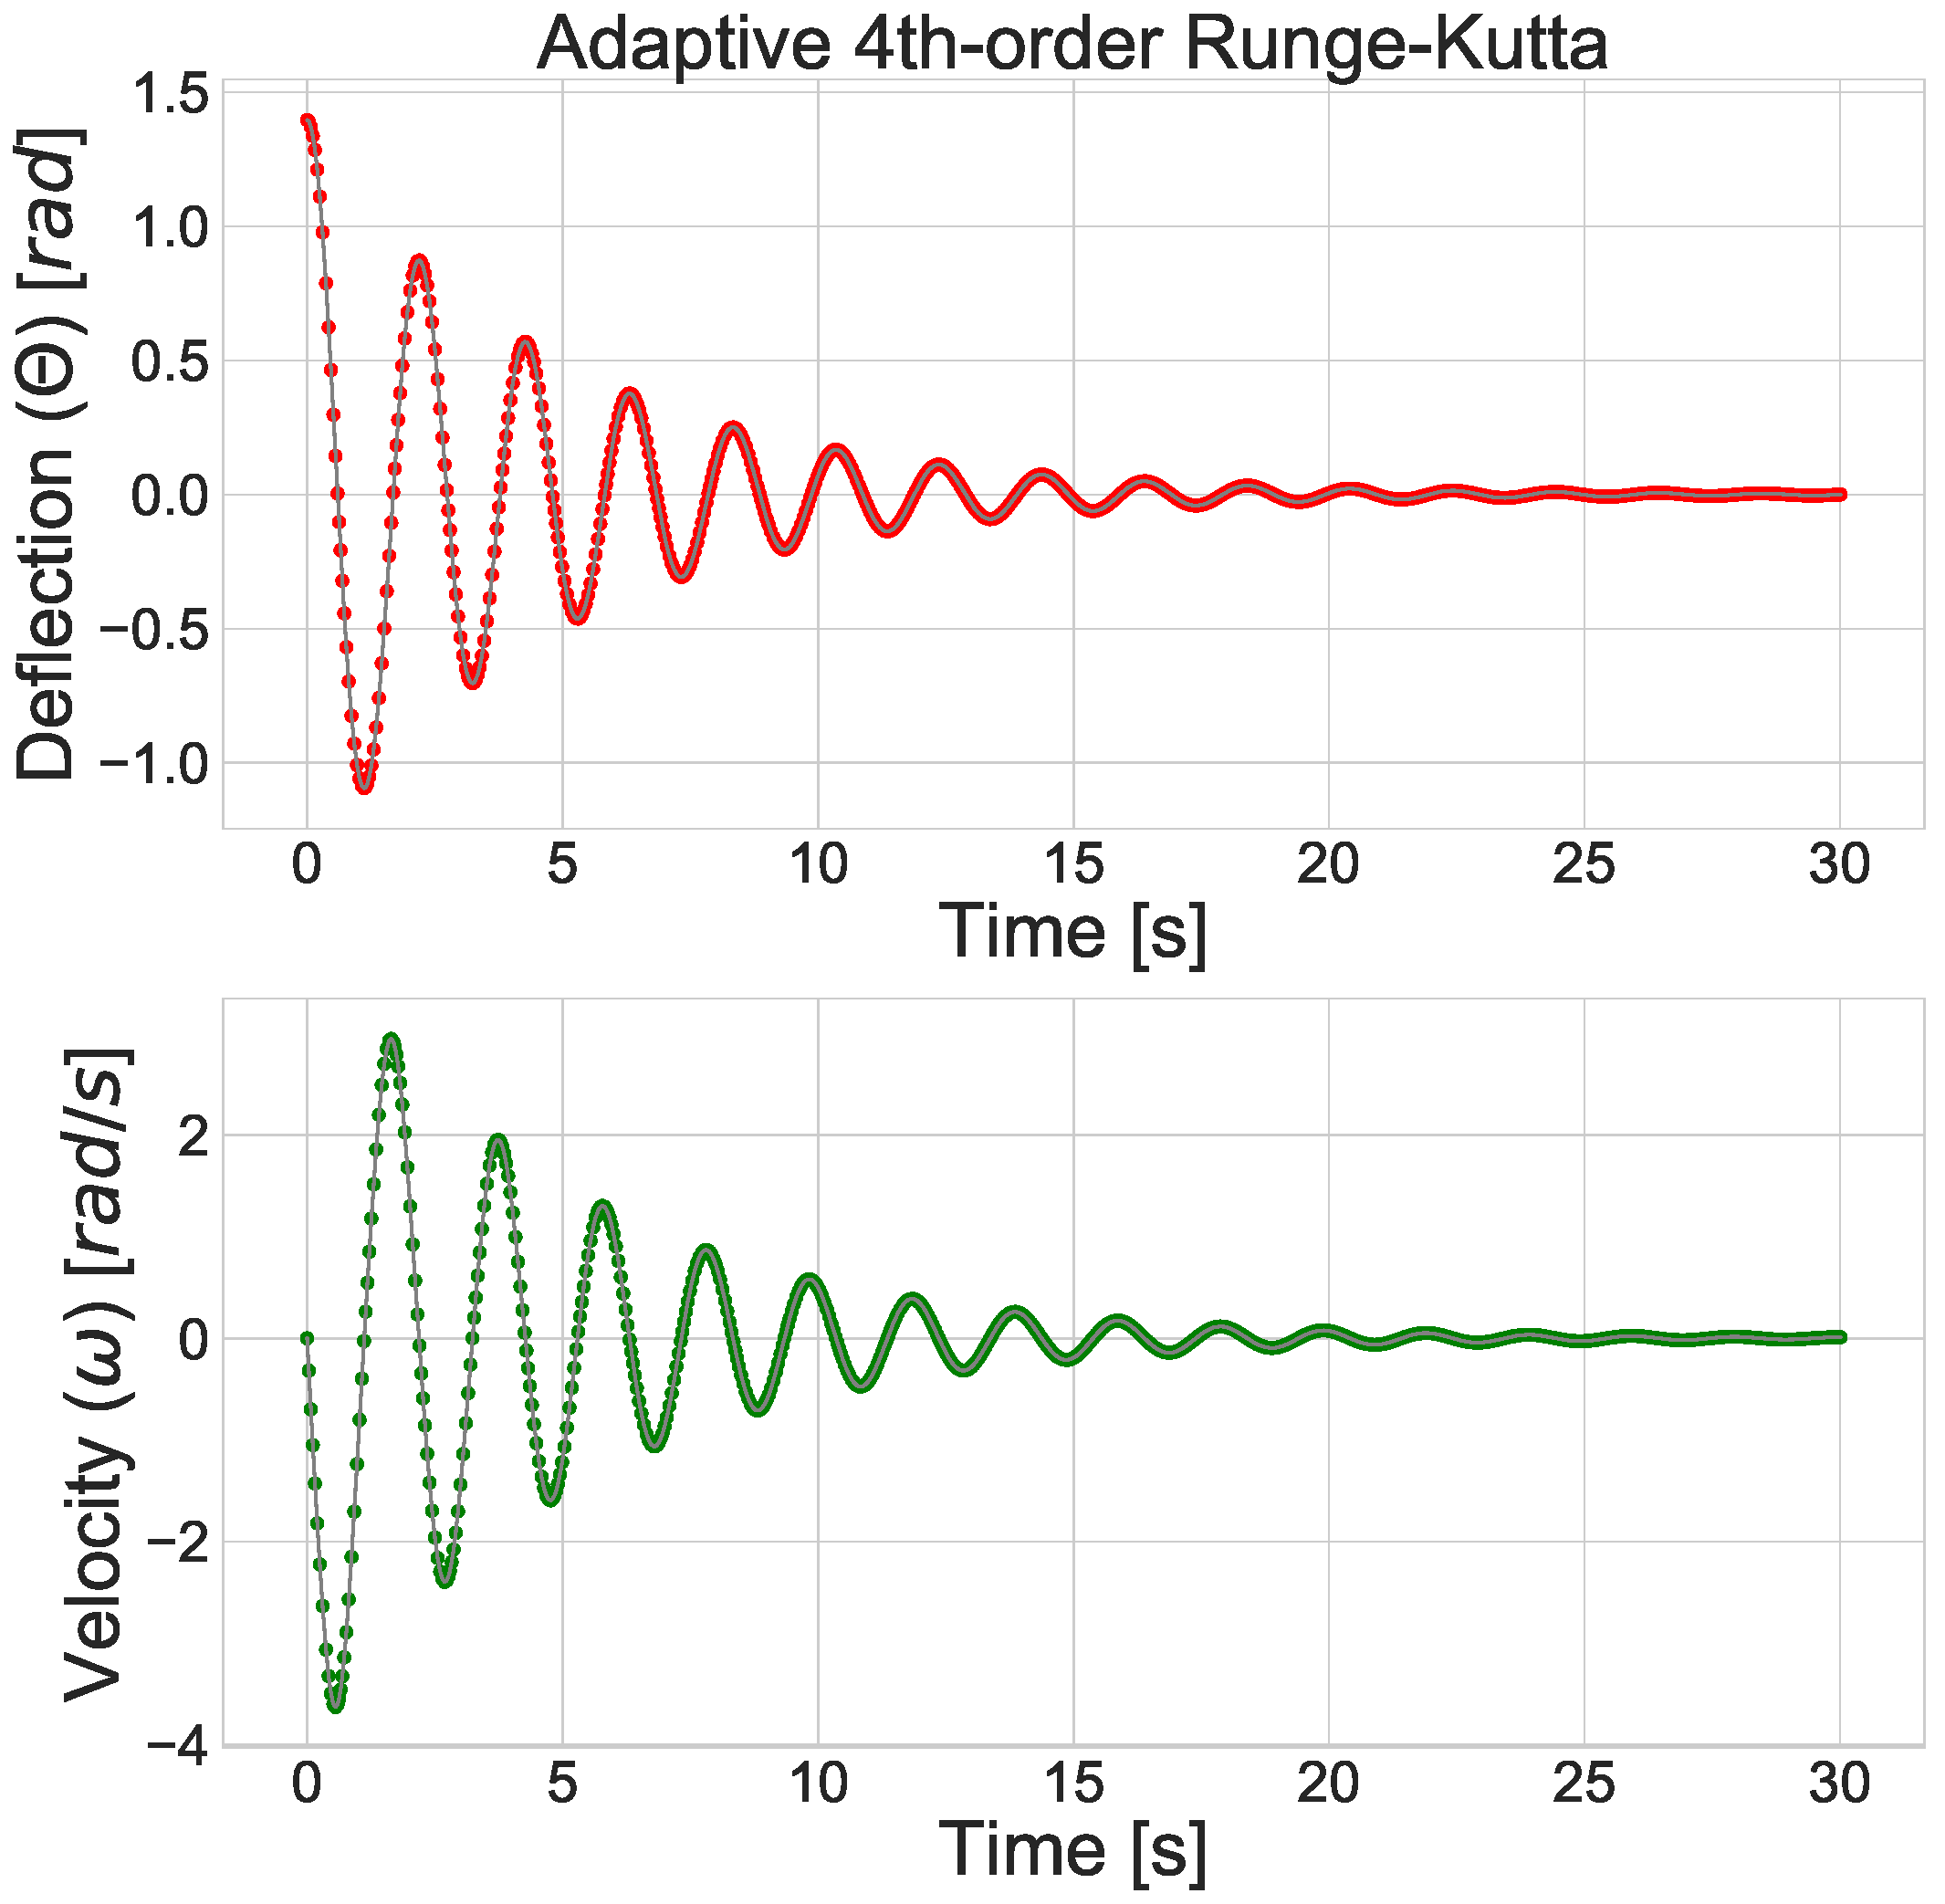
\includegraphics[width=.25\textwidth]{images/theta_omega_adapt_runge_damped.pdf}}
\captionof{figure}{Ad. Runge-Kutta\\Damp.}\label{fig:13}
\hfill
{\centering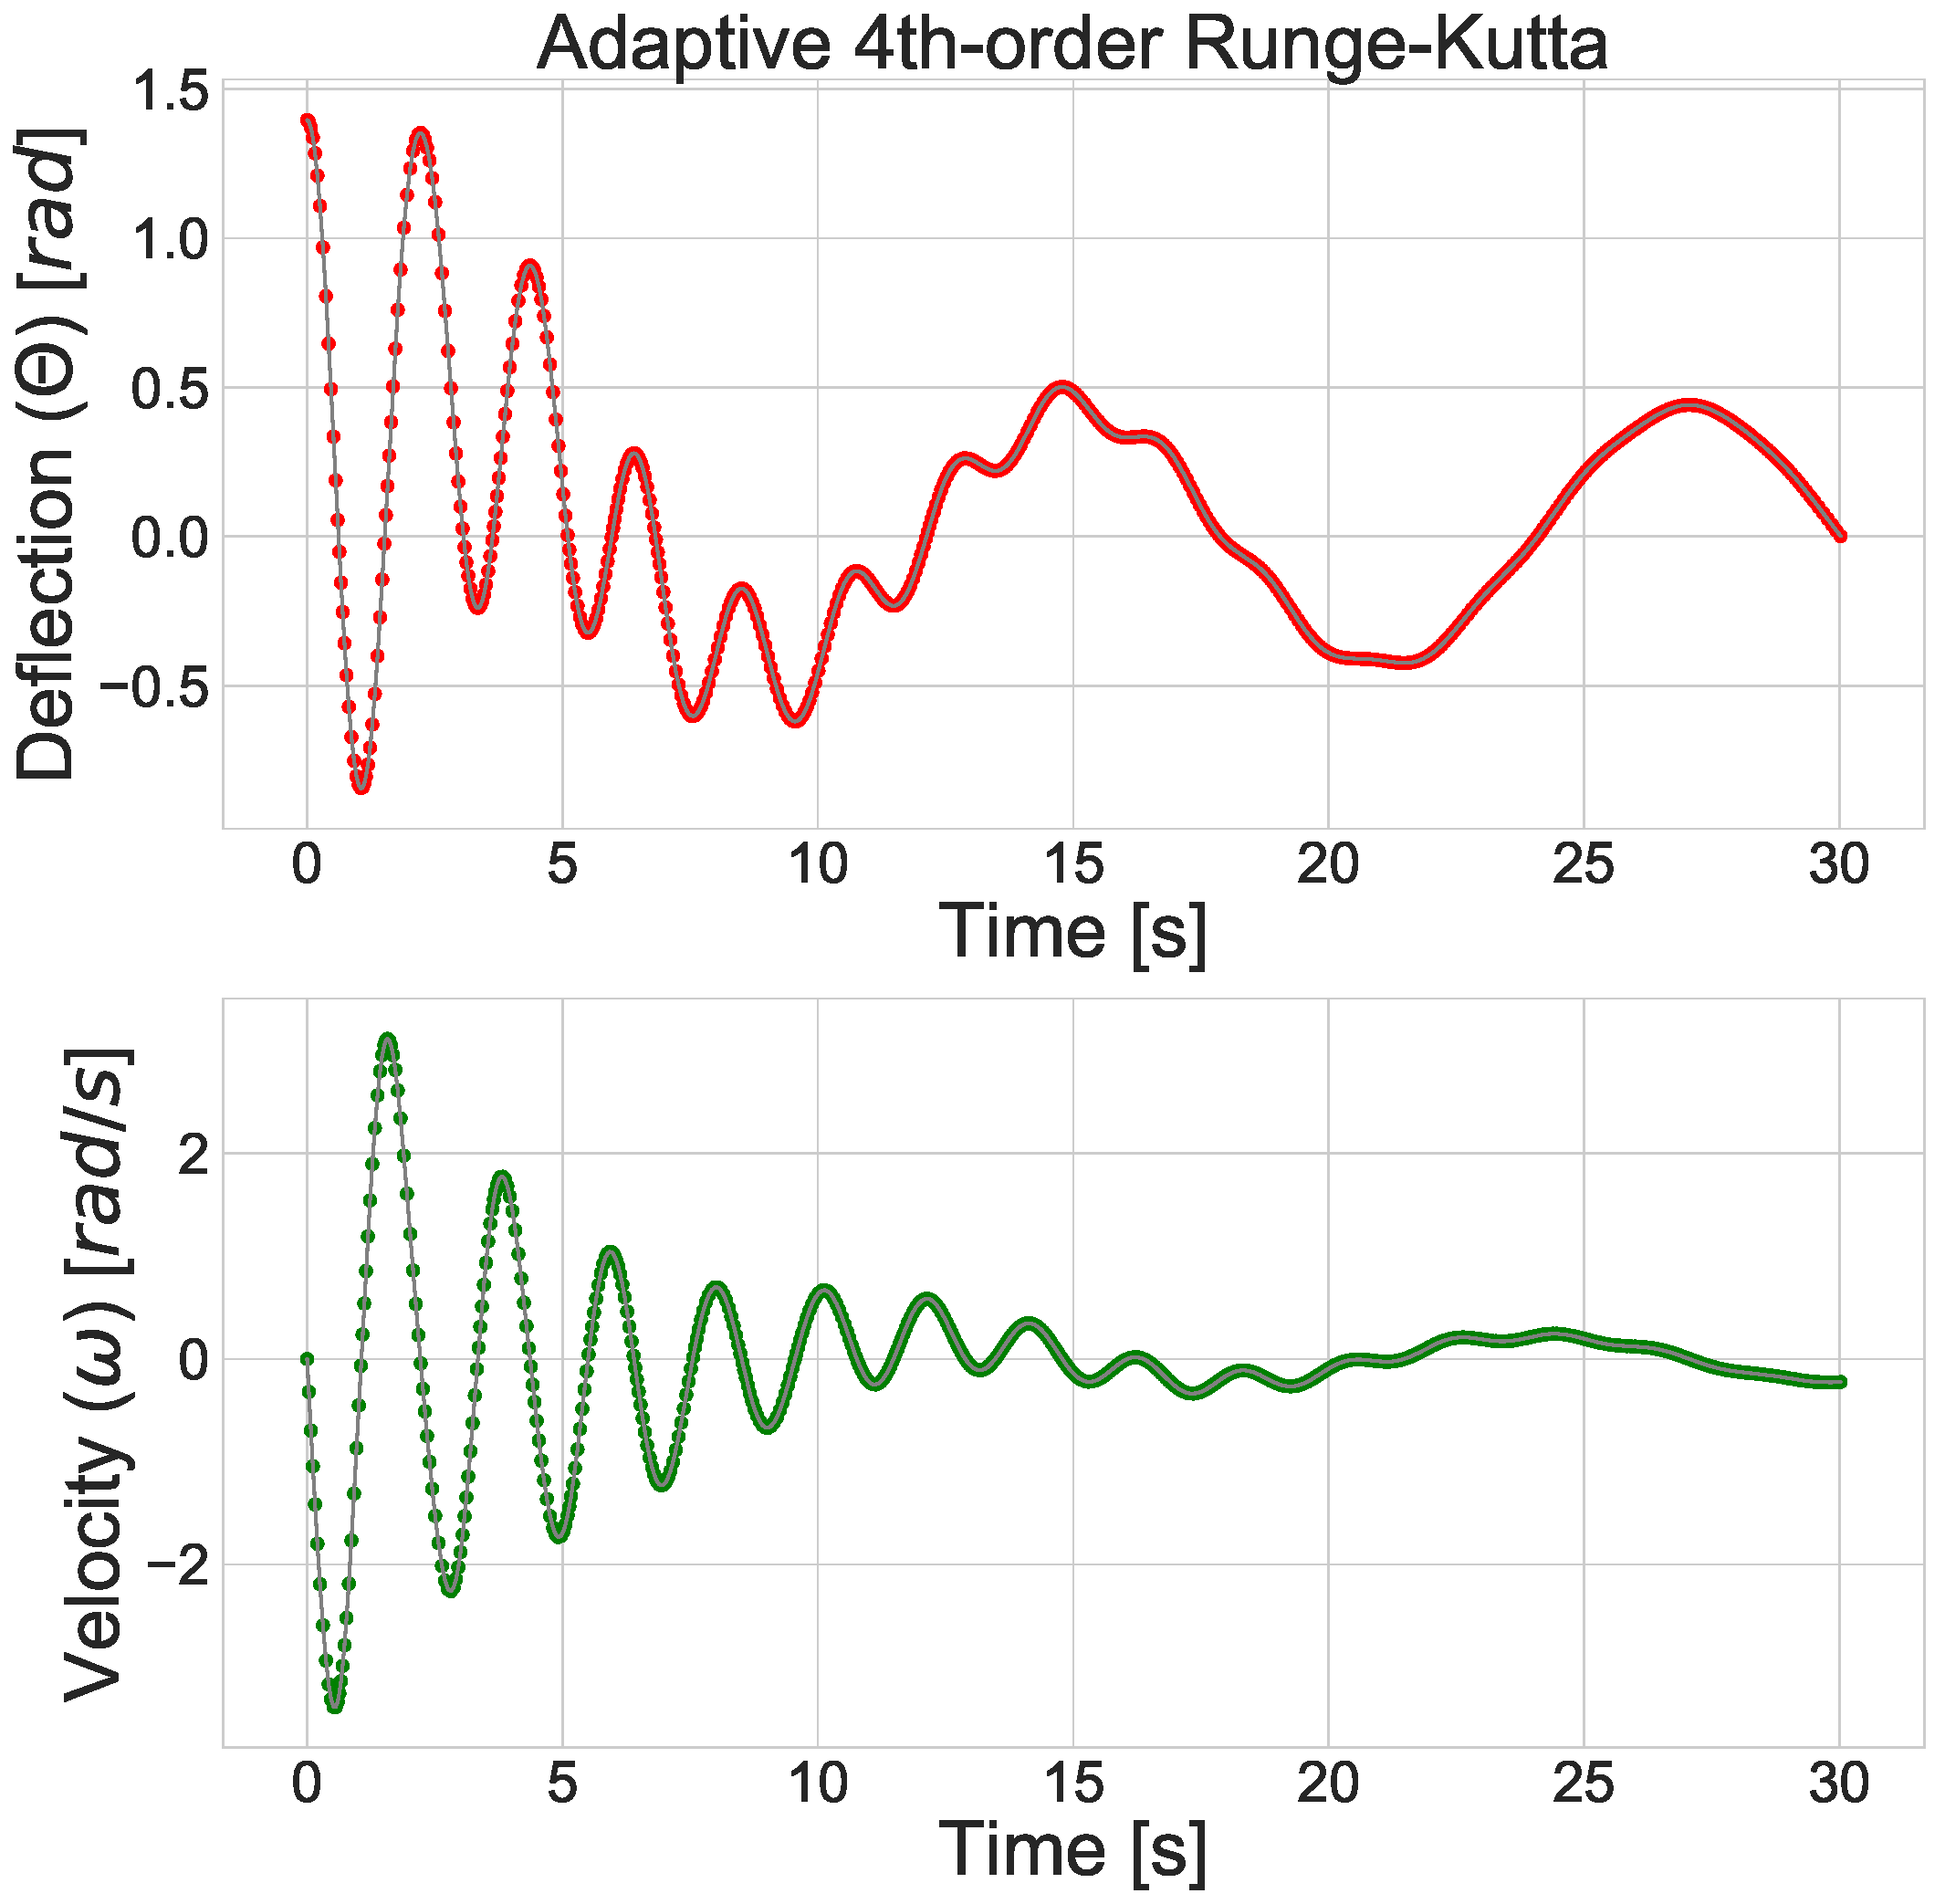
\includegraphics[width=.25\textwidth]{images/theta_omega_adapt_runge_dampeddriven.pdf}}
\captionof{figure}{Ad. Runge-Kutta\\Damp.-Driv.}\label{fig:14}
\hfill
{\centering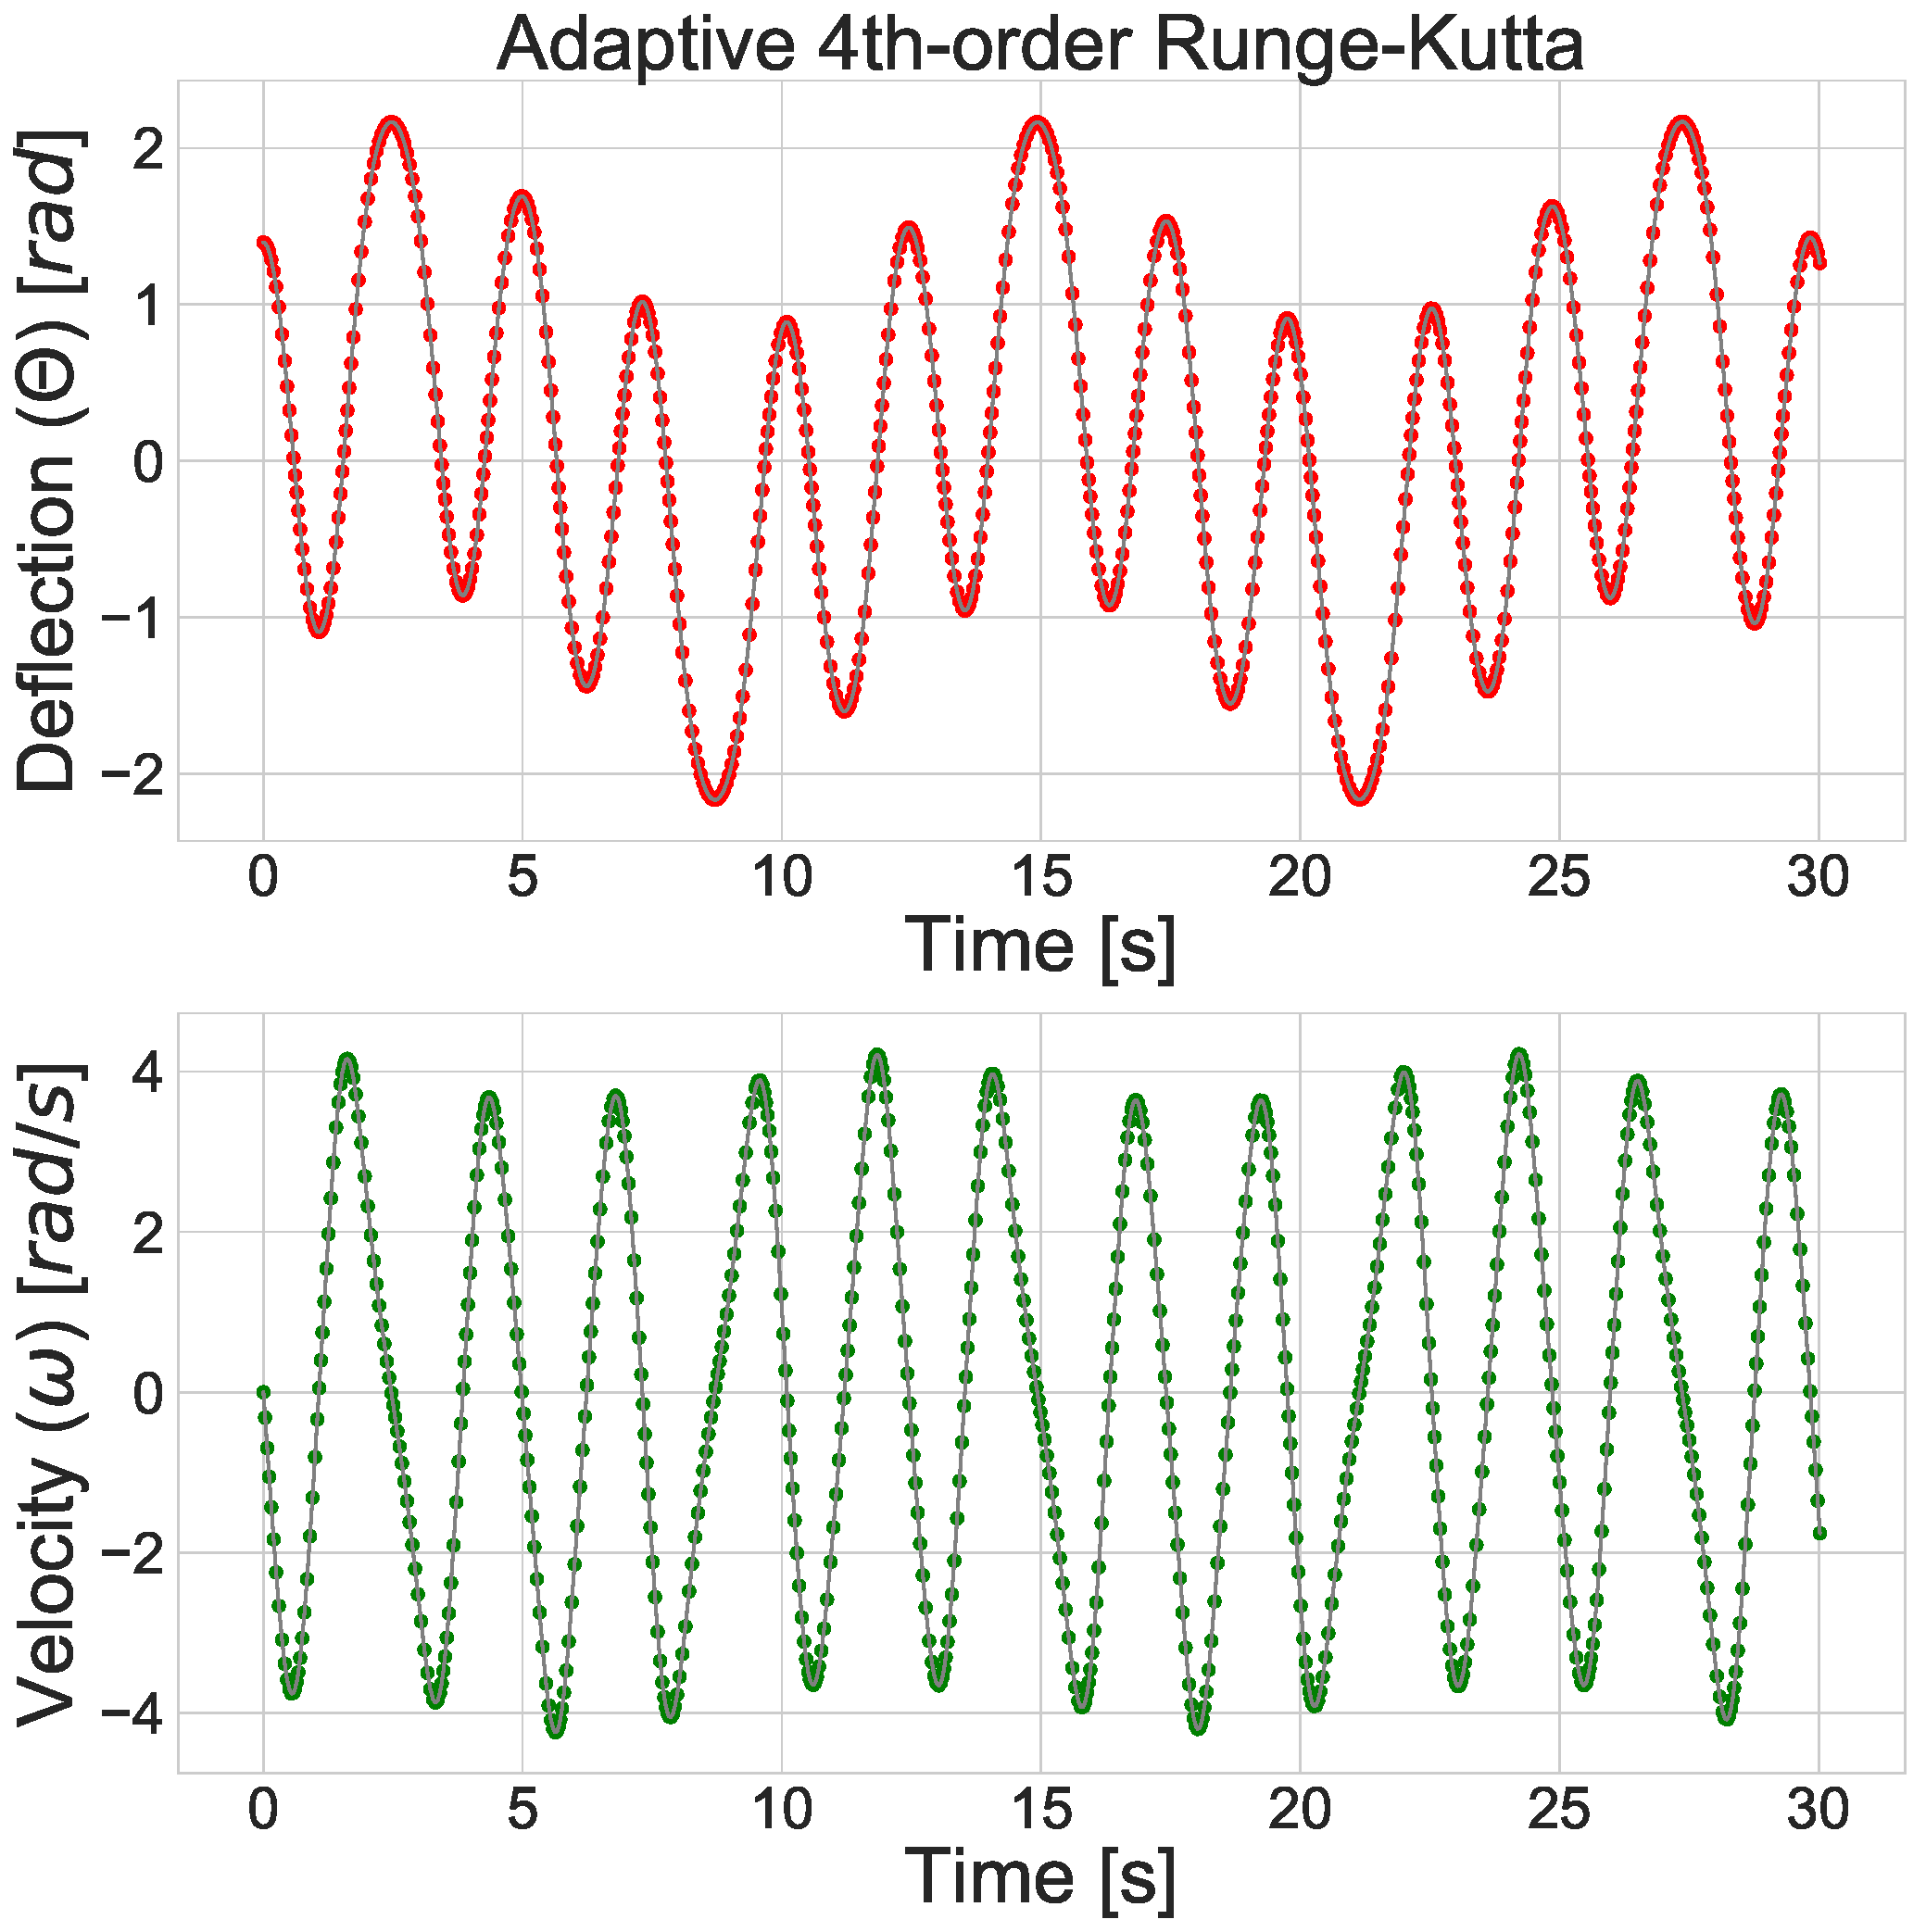
\includegraphics[width=.25\textwidth]{images/theta_omega_adapt_runge_driven.pdf}}
\captionof{figure}{Ad. Runge-Kutta\\Driv.}\label{fig:15}
\hfill

\end{multicols}
\begin{multicols}{4}

{\centering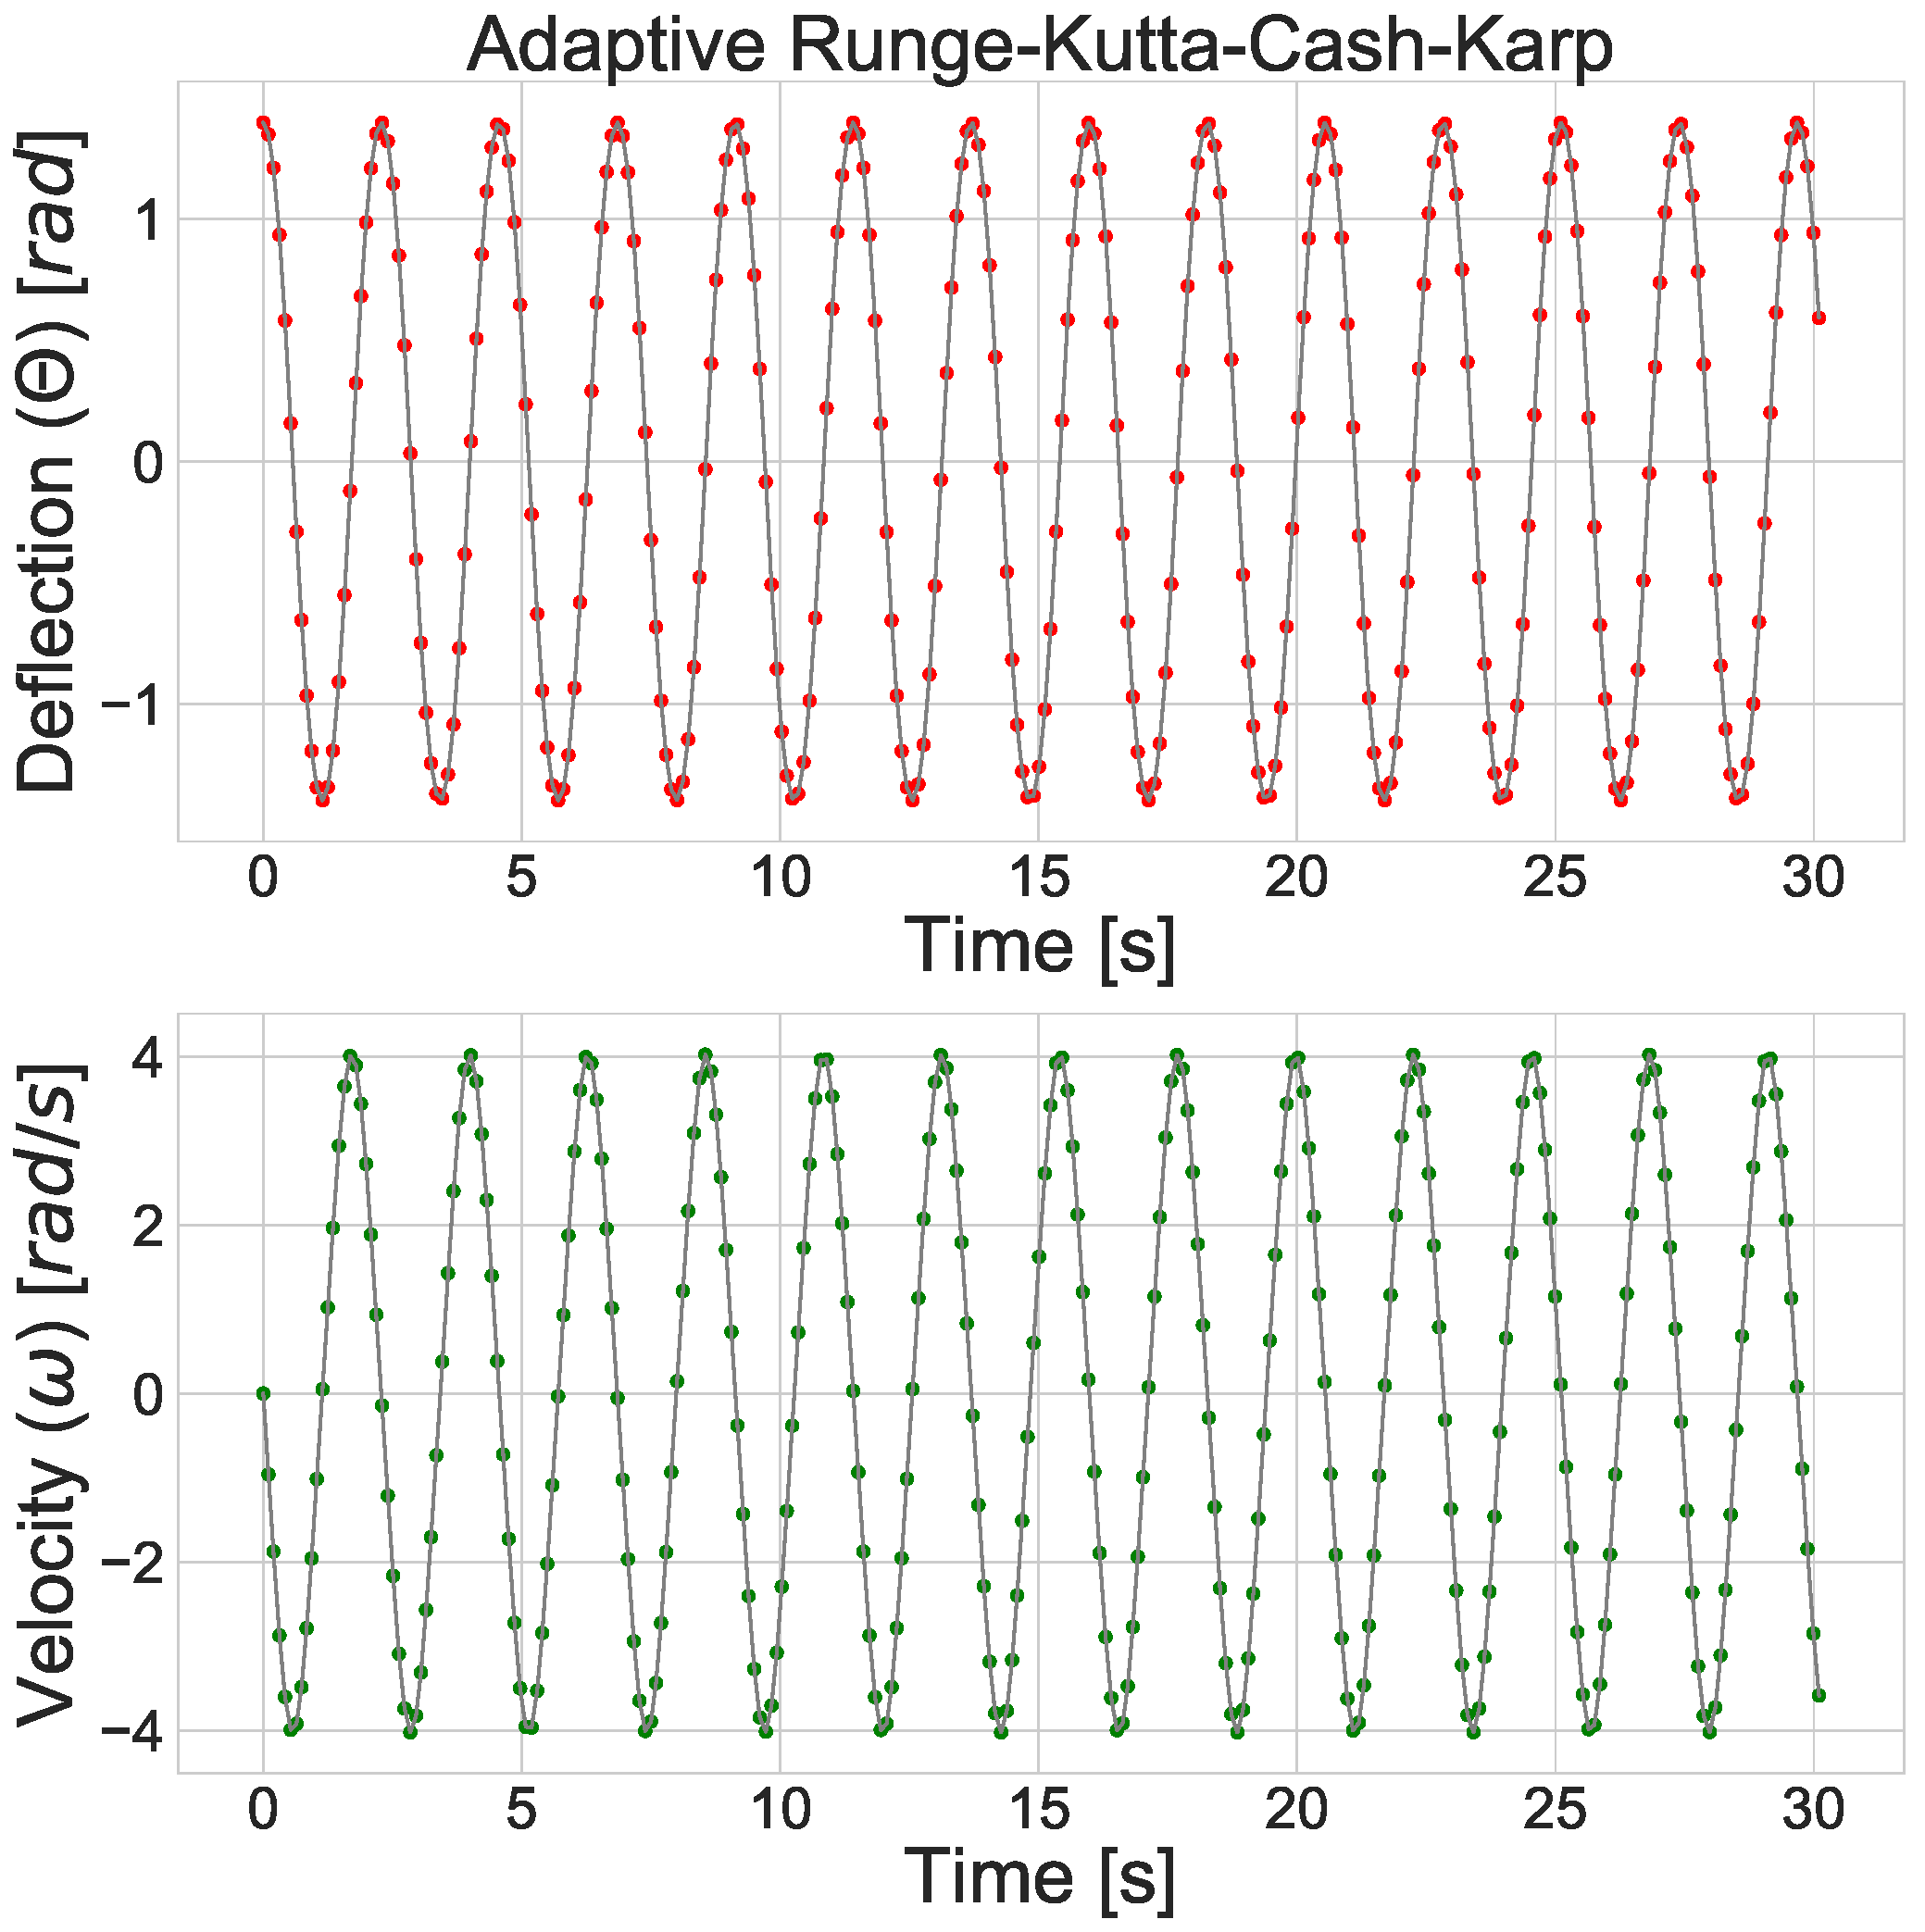
\includegraphics[width=.25\textwidth]{images/theta_omega_adapt_rkck.pdf}}
\captionof{figure}{Ad. R-K-C-K\\Mat.}\label{fig:16}
\hfill
{\centering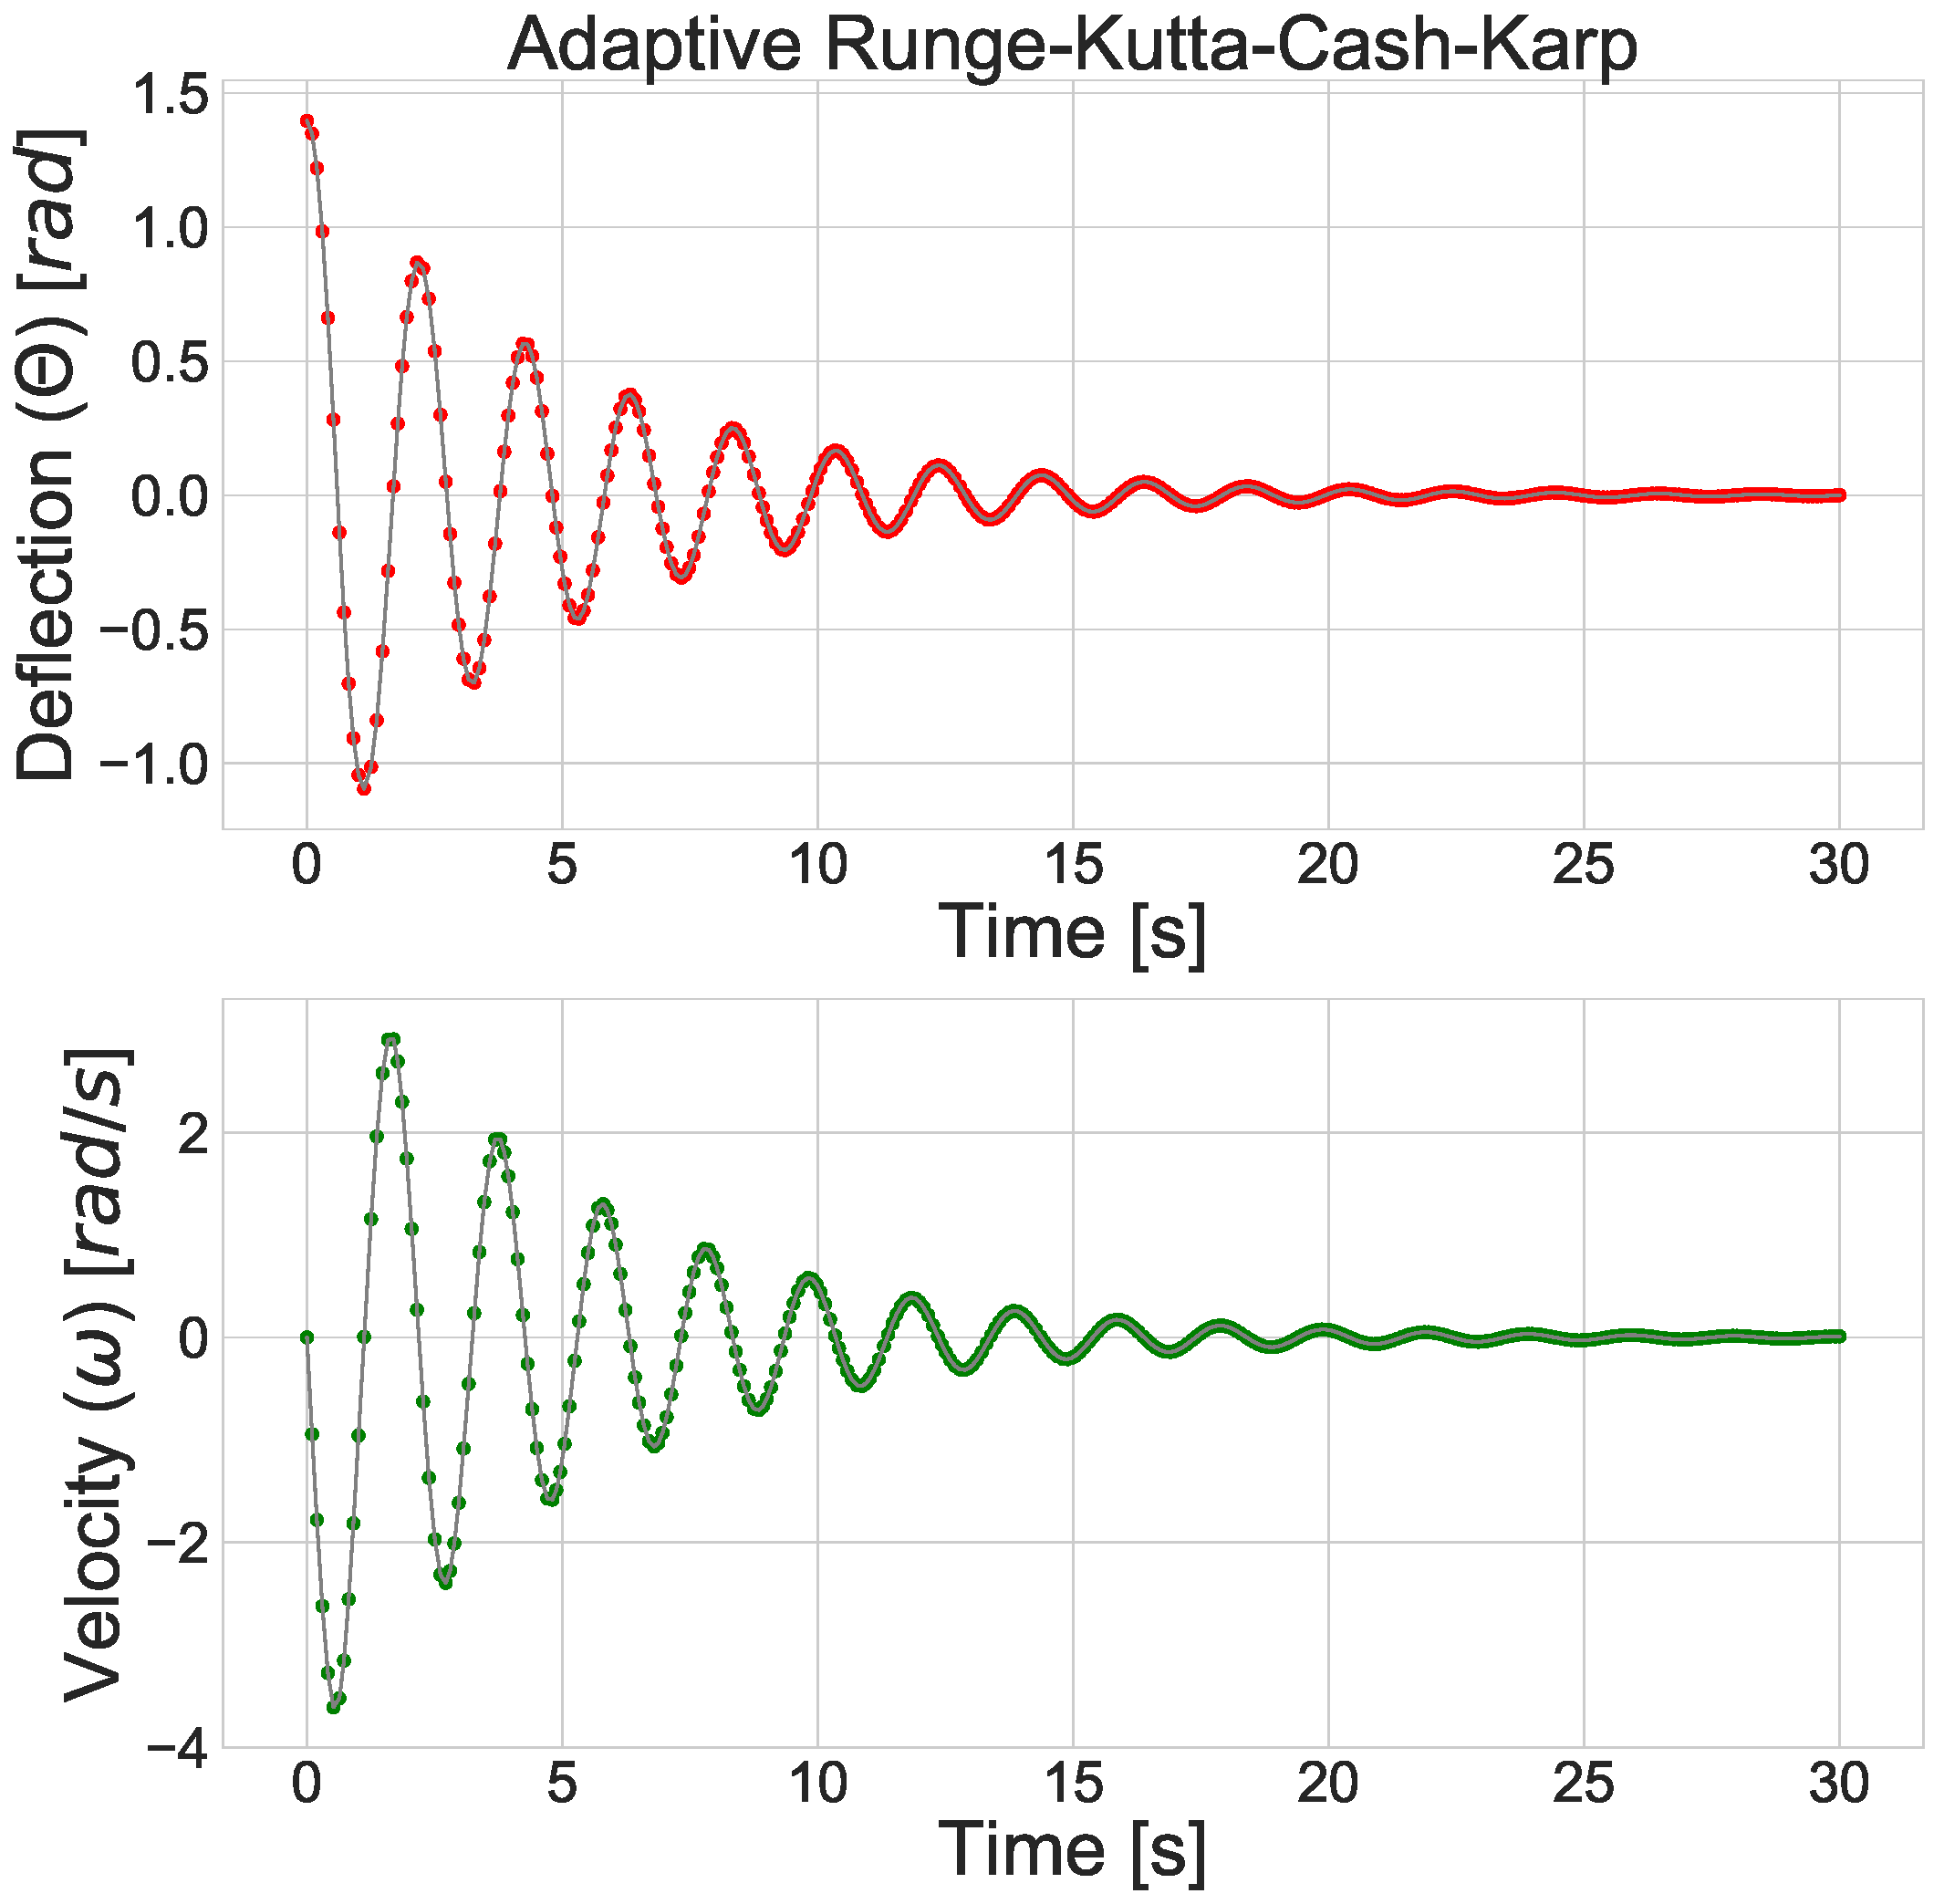
\includegraphics[width=.25\textwidth]{images/theta_omega_adapt_rkck_damped.pdf}}
\captionof{figure}{Ad. R-K-C-K\\Damp.}\label{fig:17}
\hfill
{\centering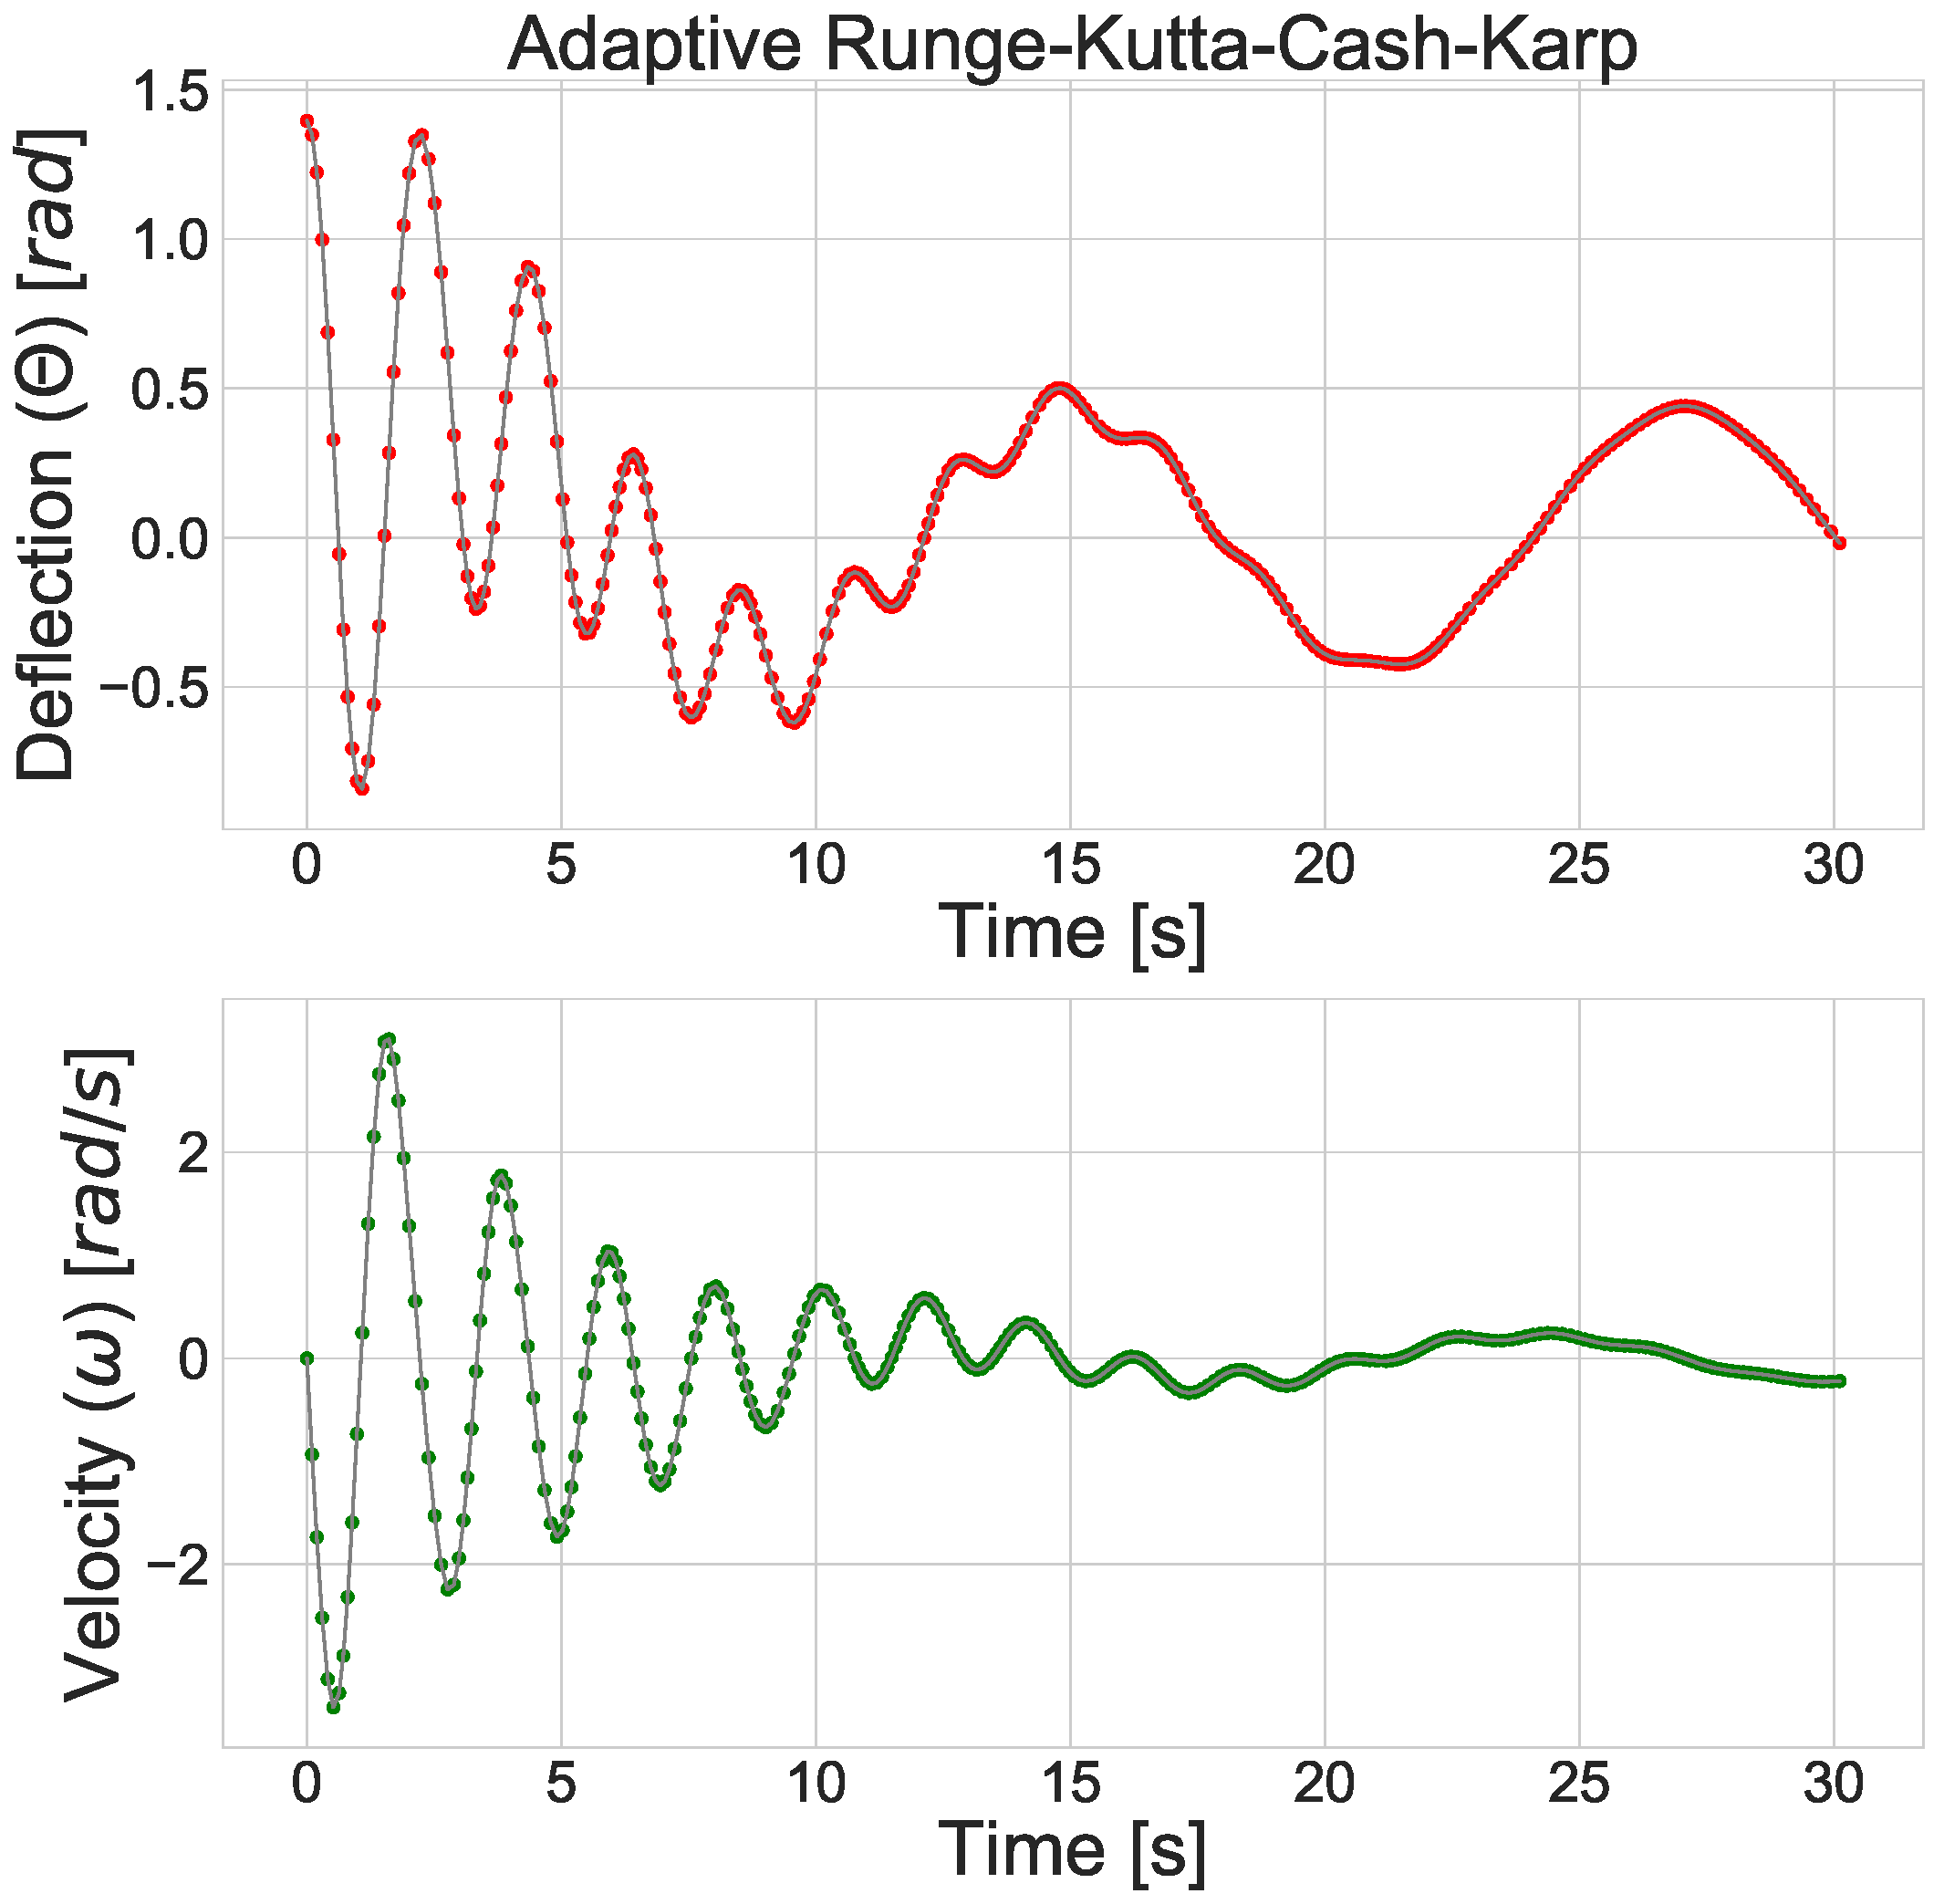
\includegraphics[width=.25\textwidth]{images/theta_omega_adapt_rkck_dampeddriven.pdf}}
\captionof{figure}{Ad. R-K-C-K\\Damp.-Driv.}\label{fig:18}
\hfill
{\centering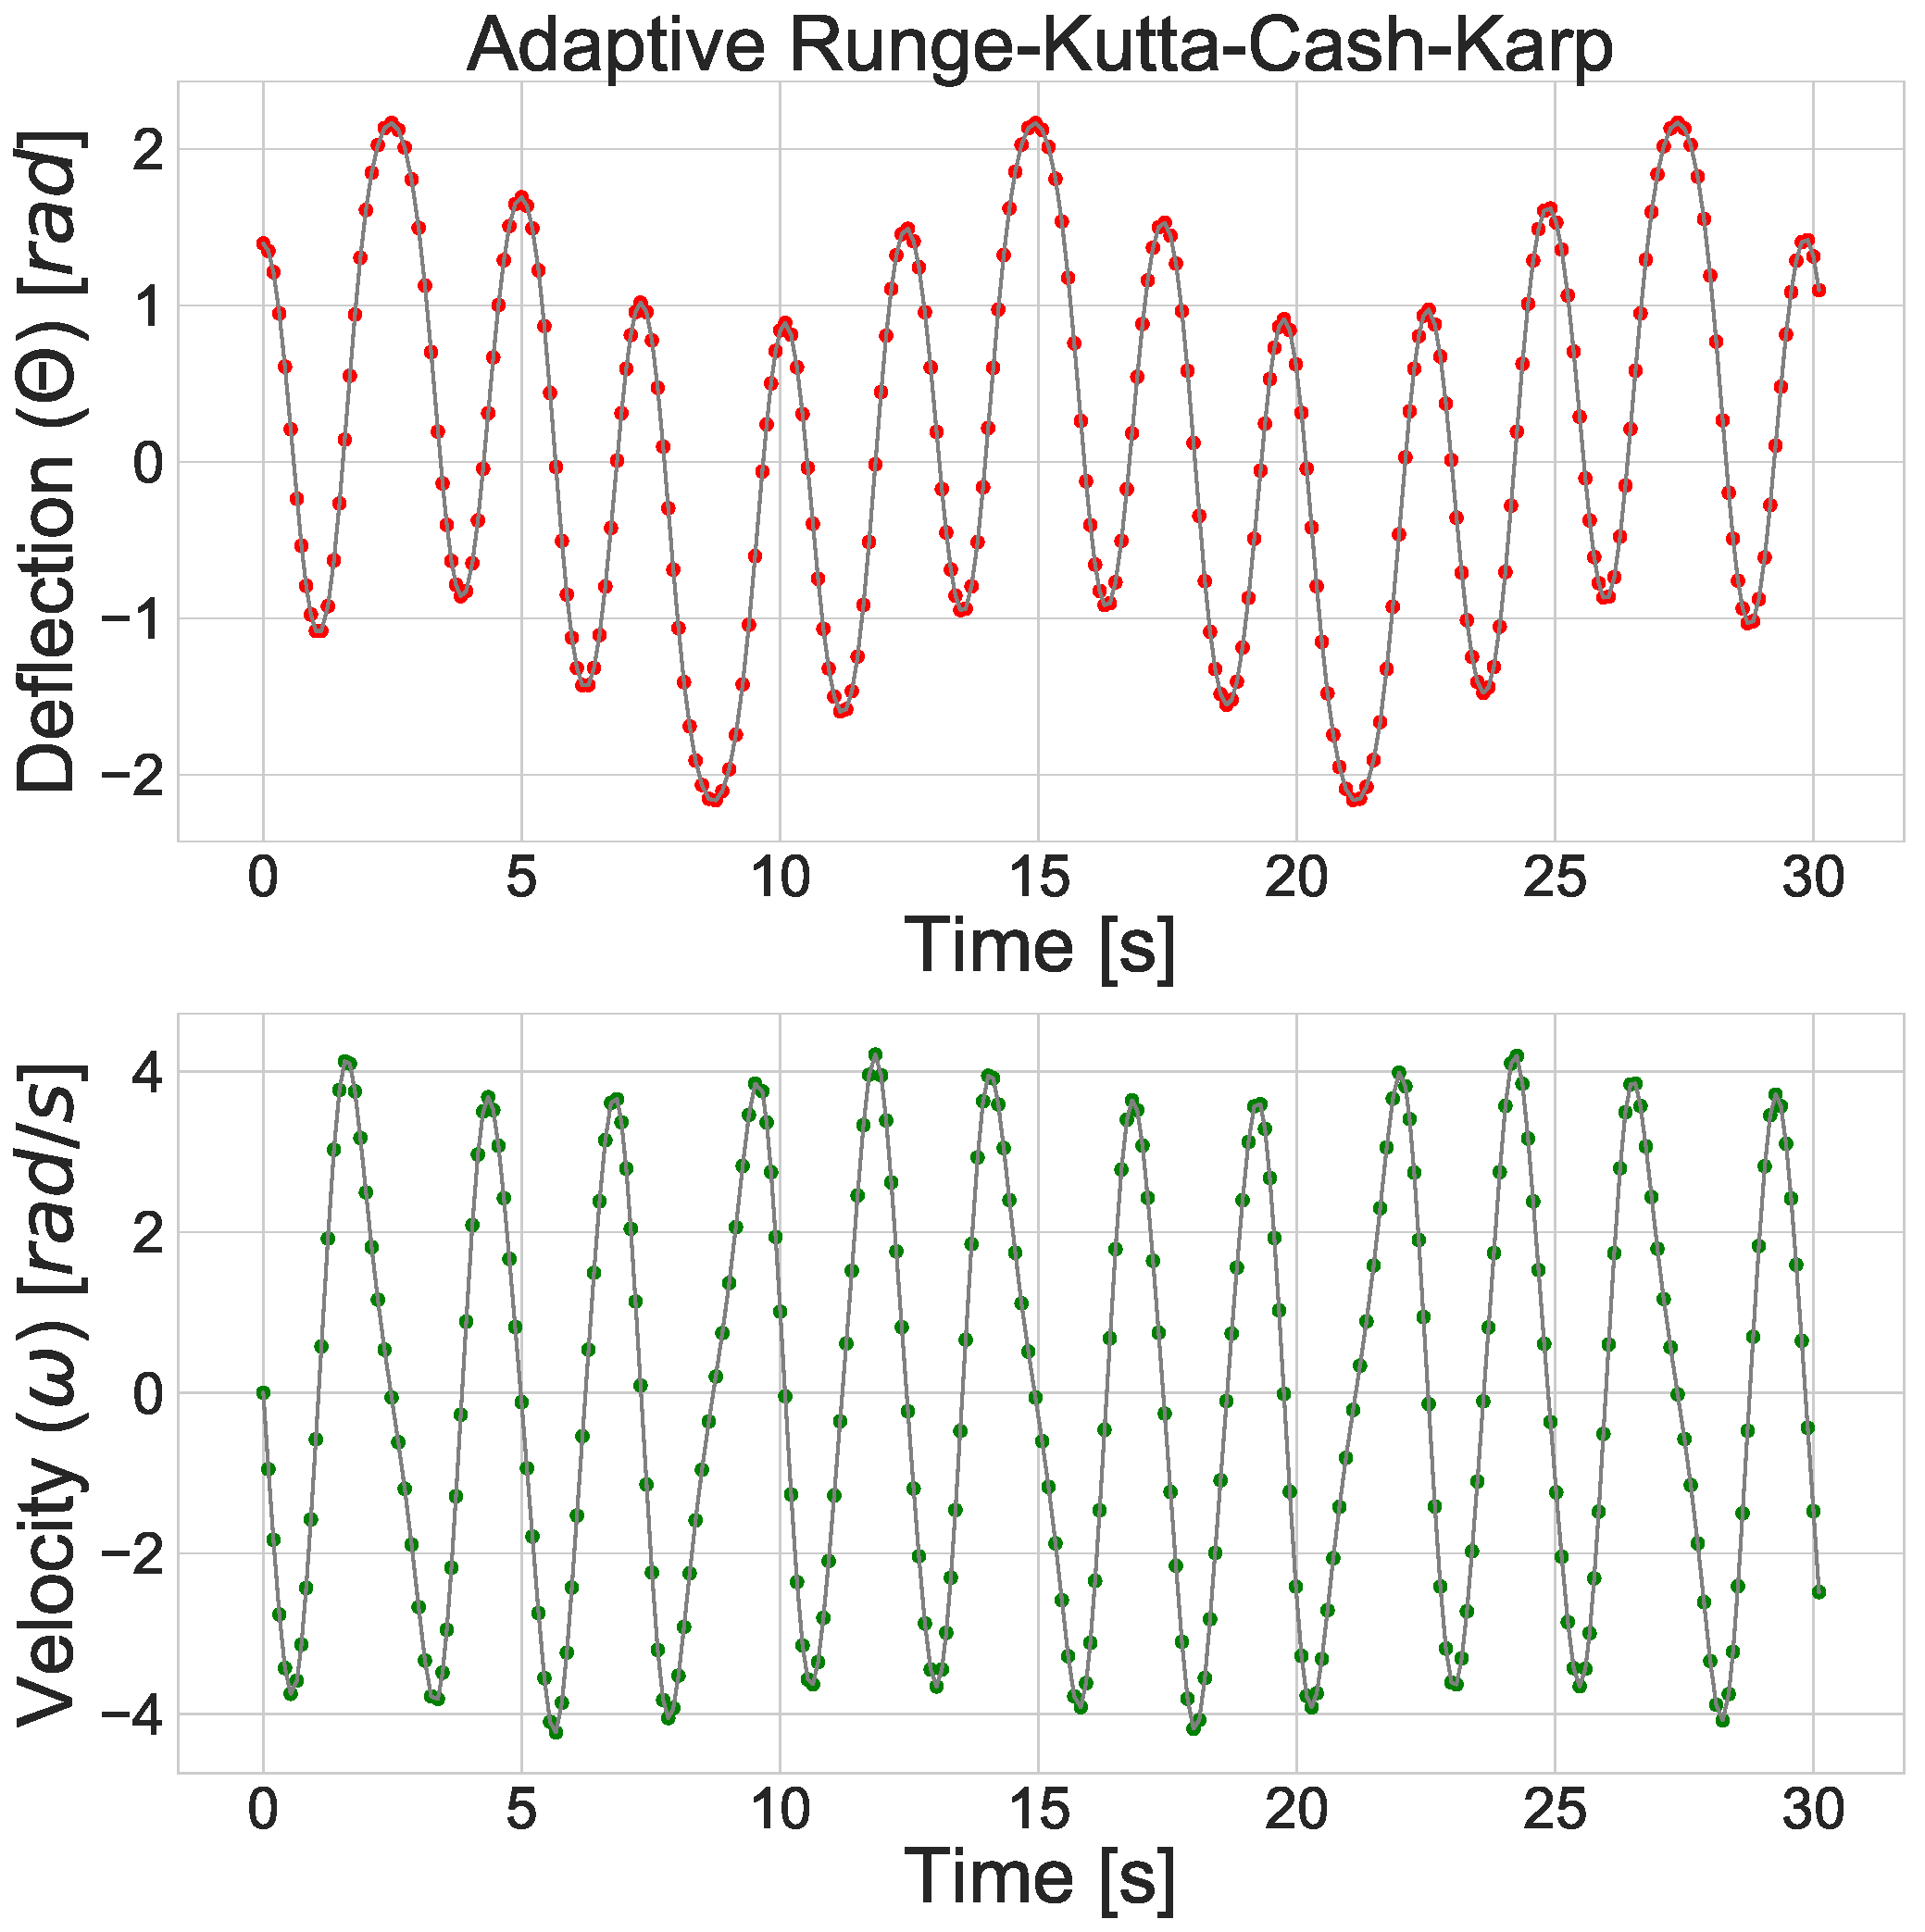
\includegraphics[width=.25\textwidth]{images/theta_omega_adapt_rkck_driven.pdf}}
\captionof{figure}{Ad. R-K-C-K\\Driv.}\label{fig:19}
\hfill

\end{multicols}

\newpage

\begin{multicols}{4}

{\centering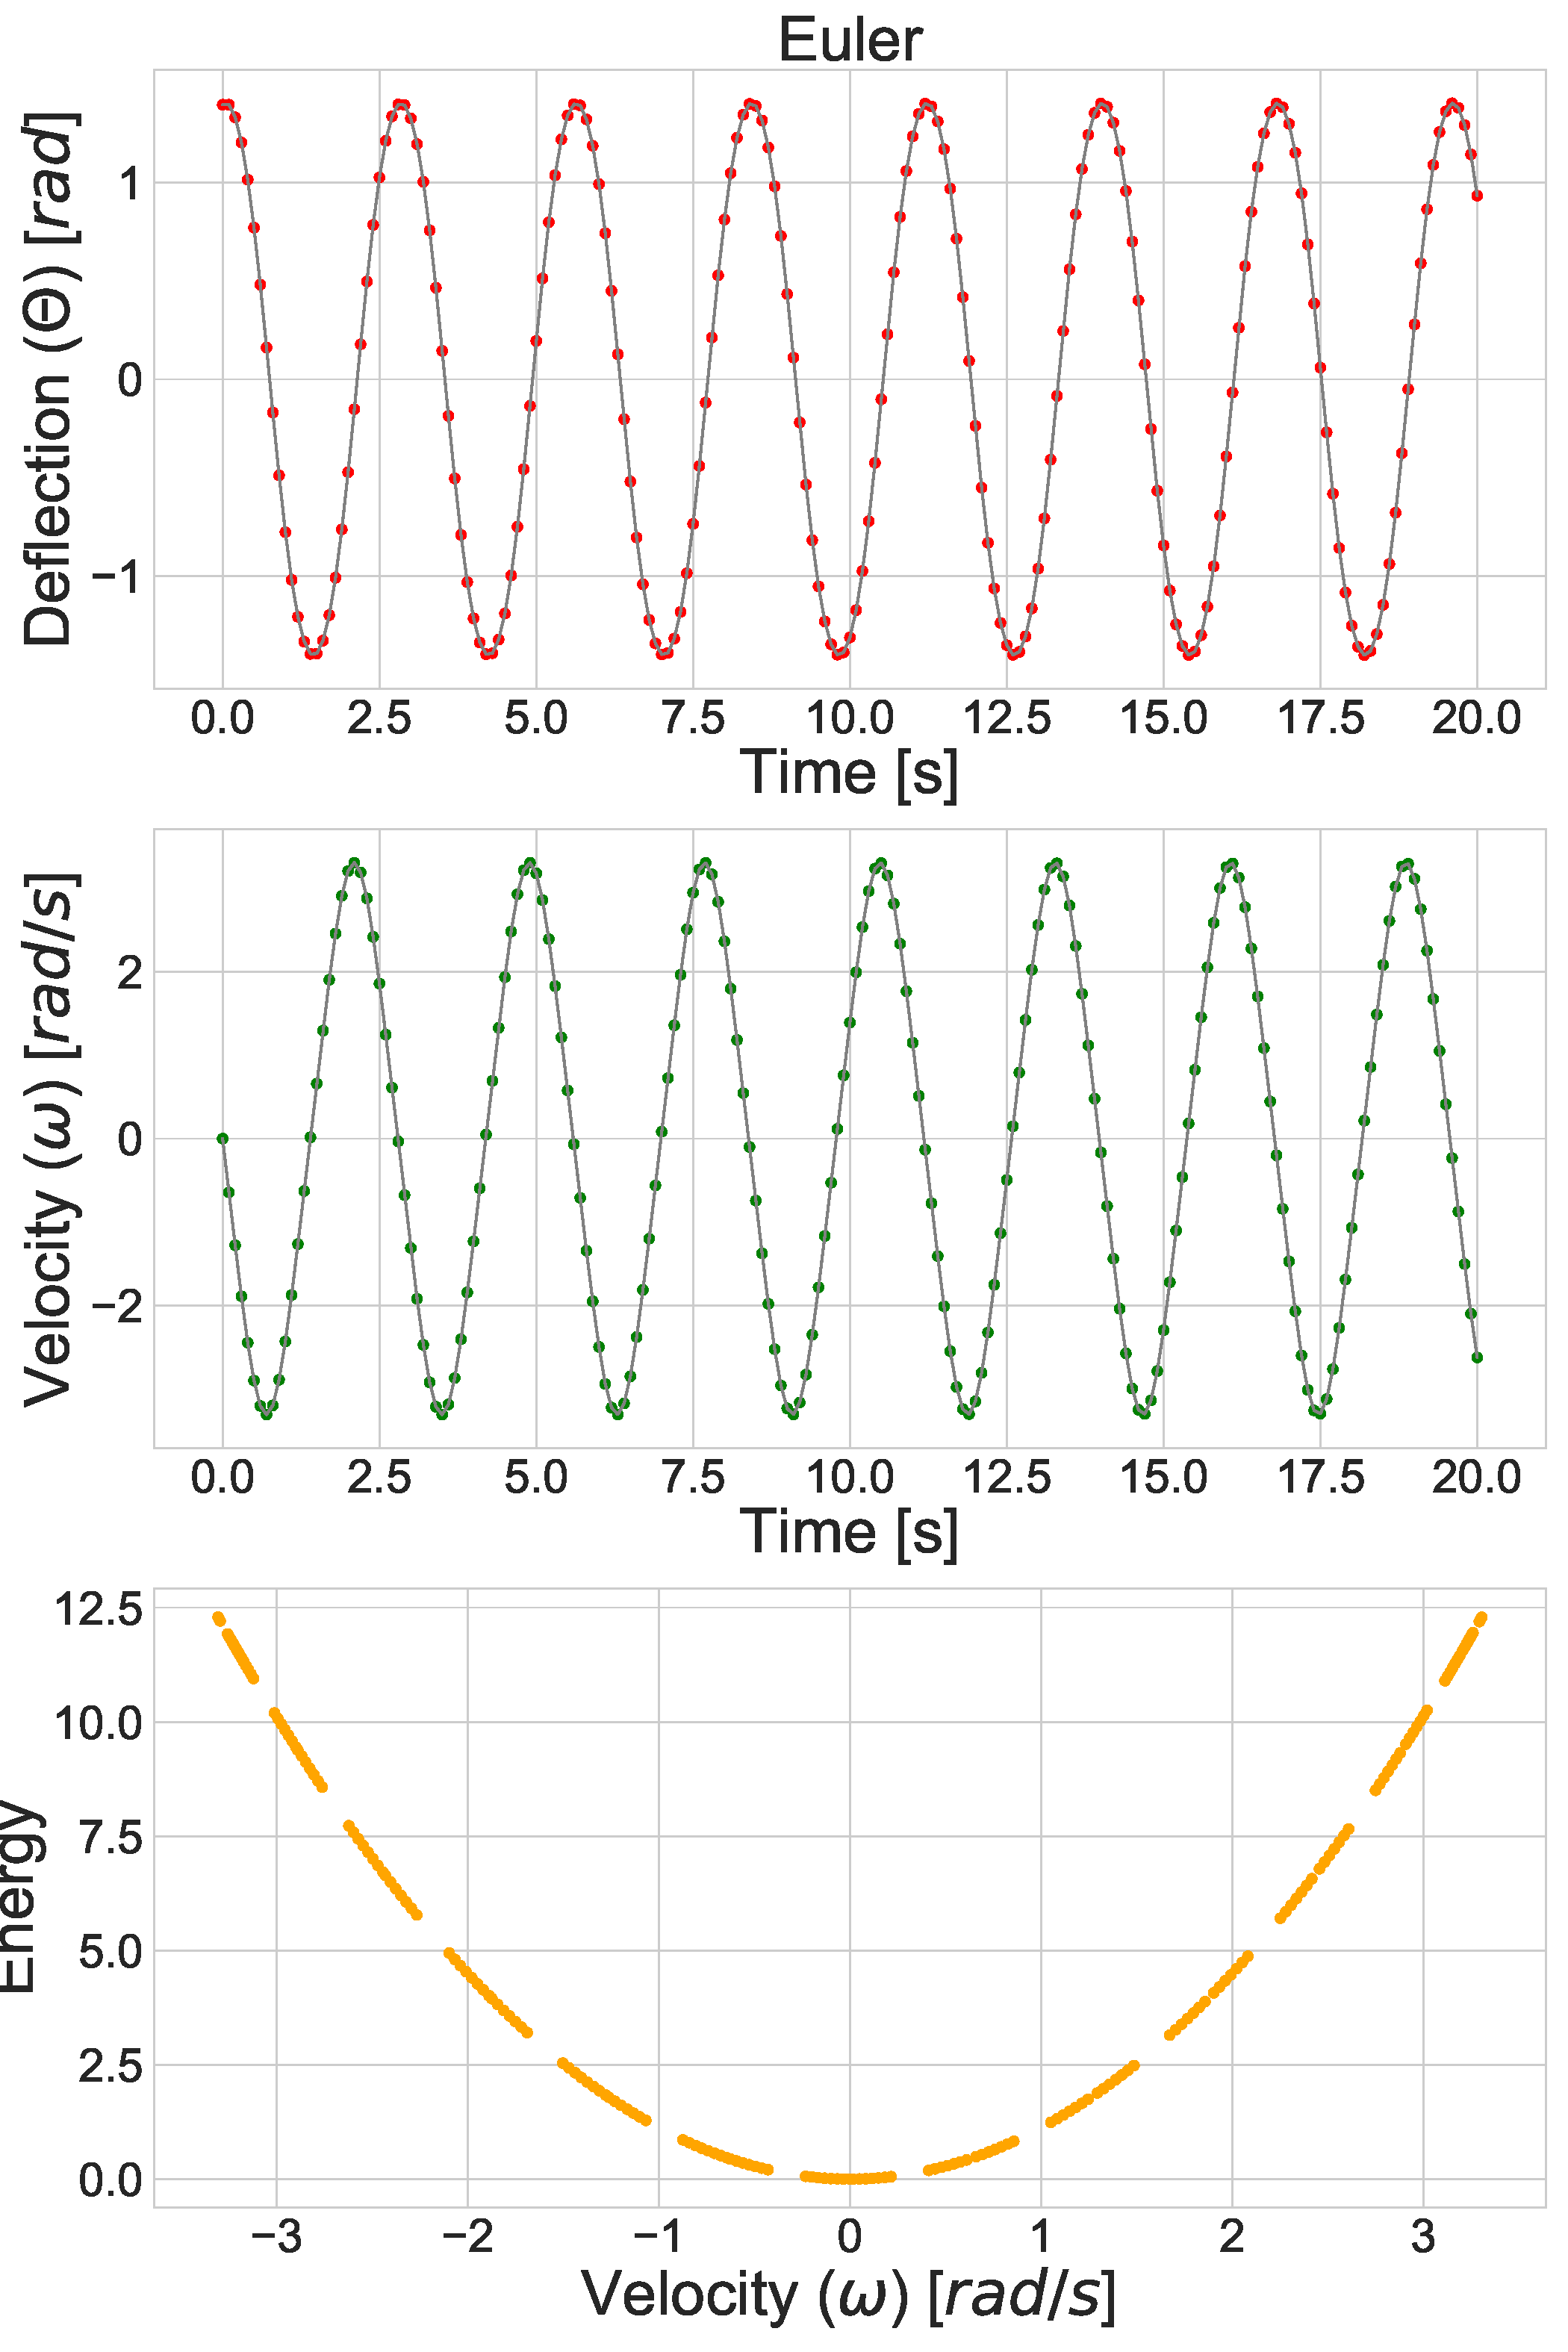
\includegraphics[width=.25\textwidth]{images/theta_omega_euler.pdf}}
\captionof{figure}{Euler\\Mat.}\label{fig:20}
\hfill
{\centering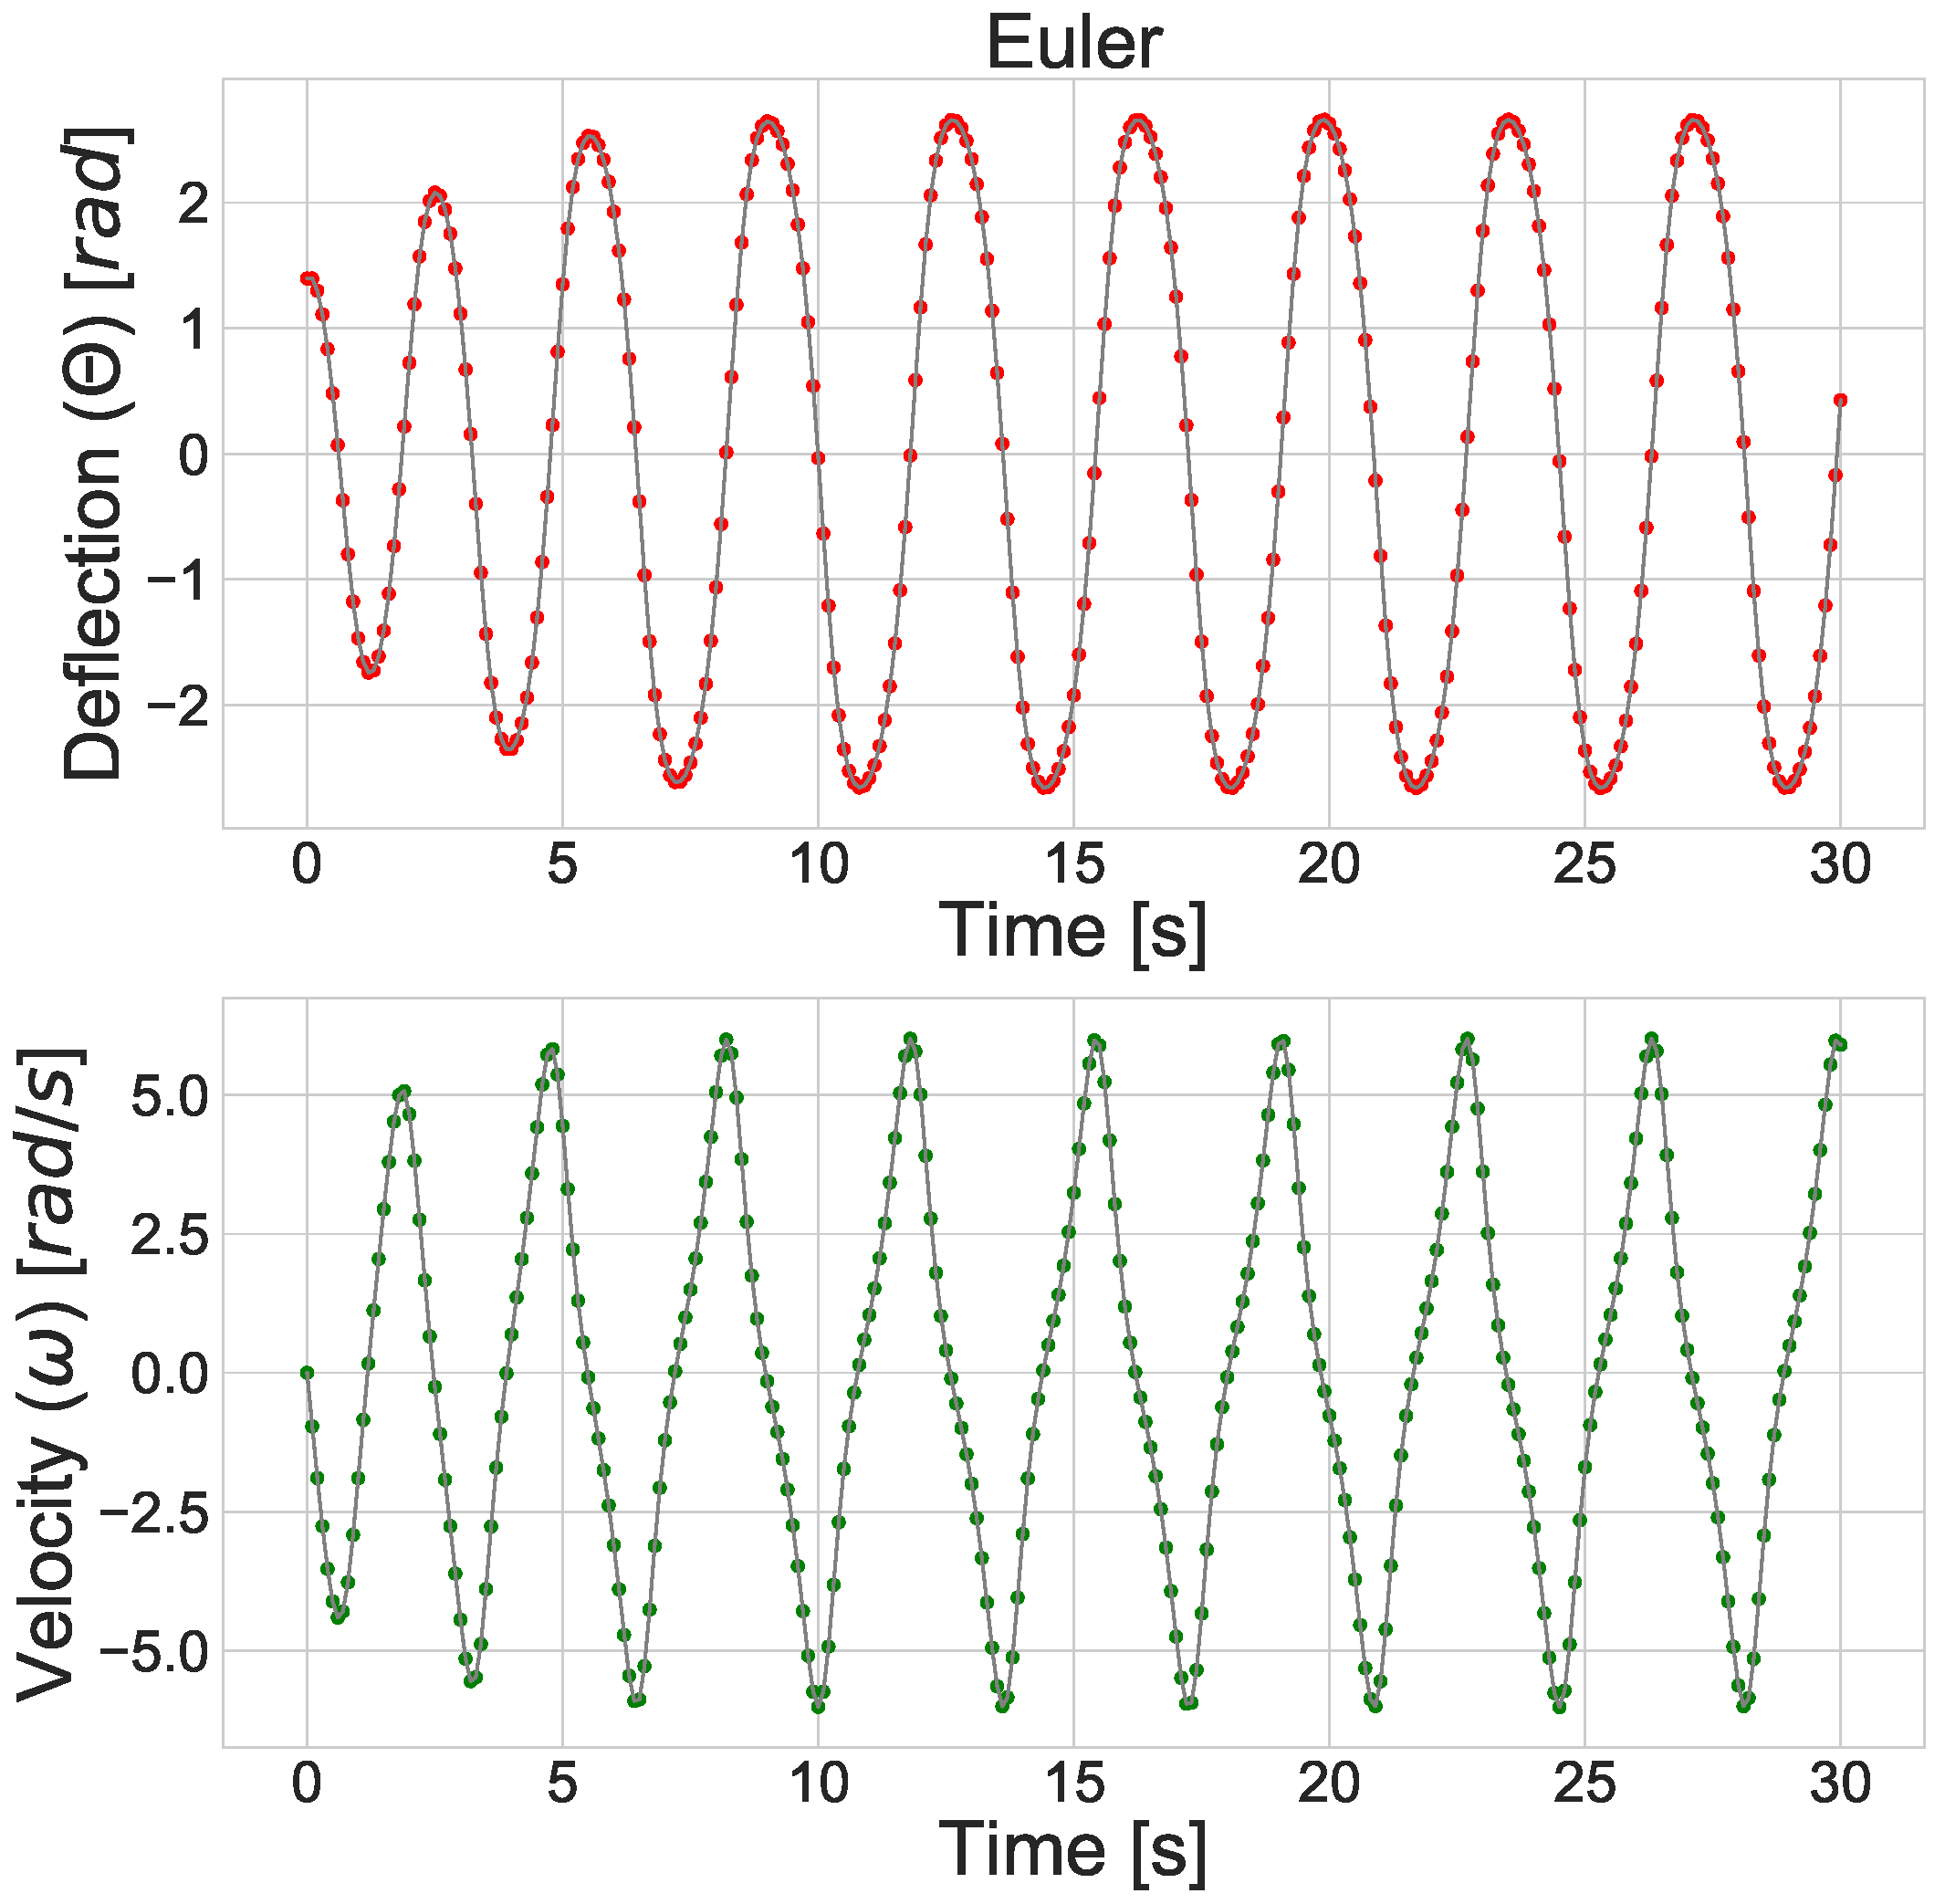
\includegraphics[width=.25\textwidth]{images/theta_omega_euler_damped.pdf}}
\captionof{figure}{Euler\\Damp.}\label{fig:21}
\hfill
{\centering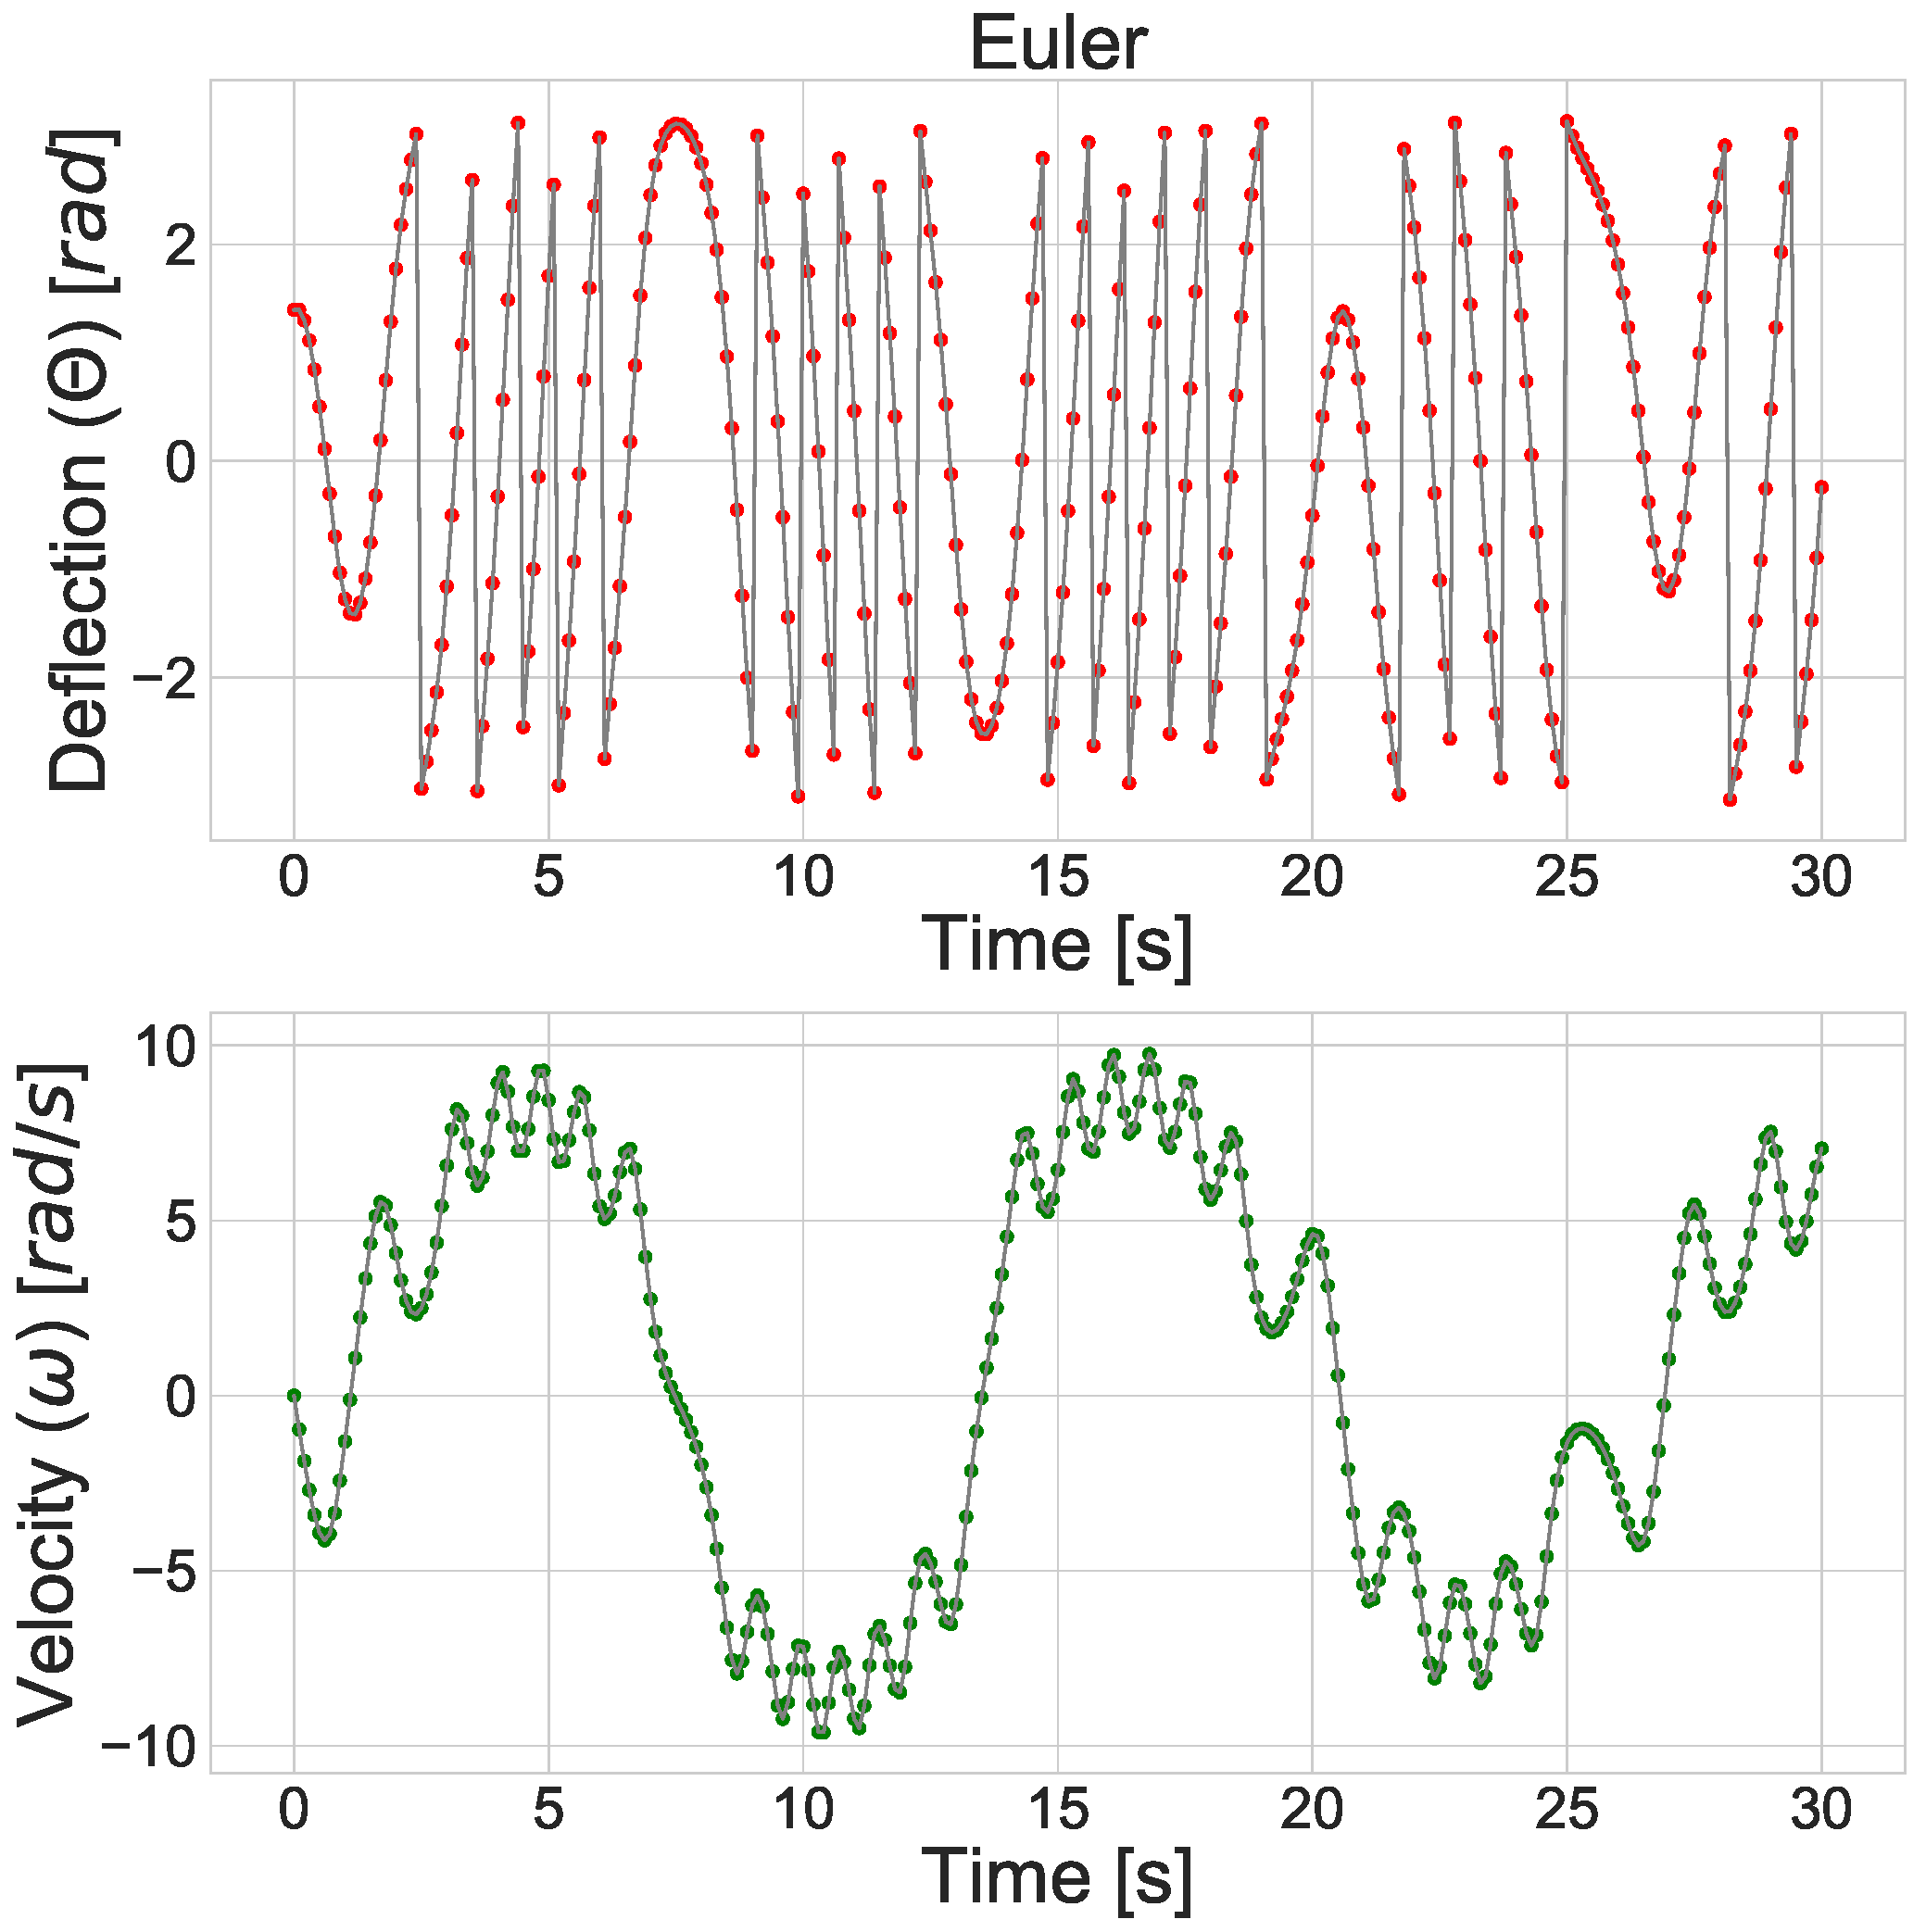
\includegraphics[width=.25\textwidth]{images/theta_omega_euler_dampeddriven.pdf}}
\captionof{figure}{Euler\\Damp.-Driv.}\label{fig:22}
\hfill
{\centering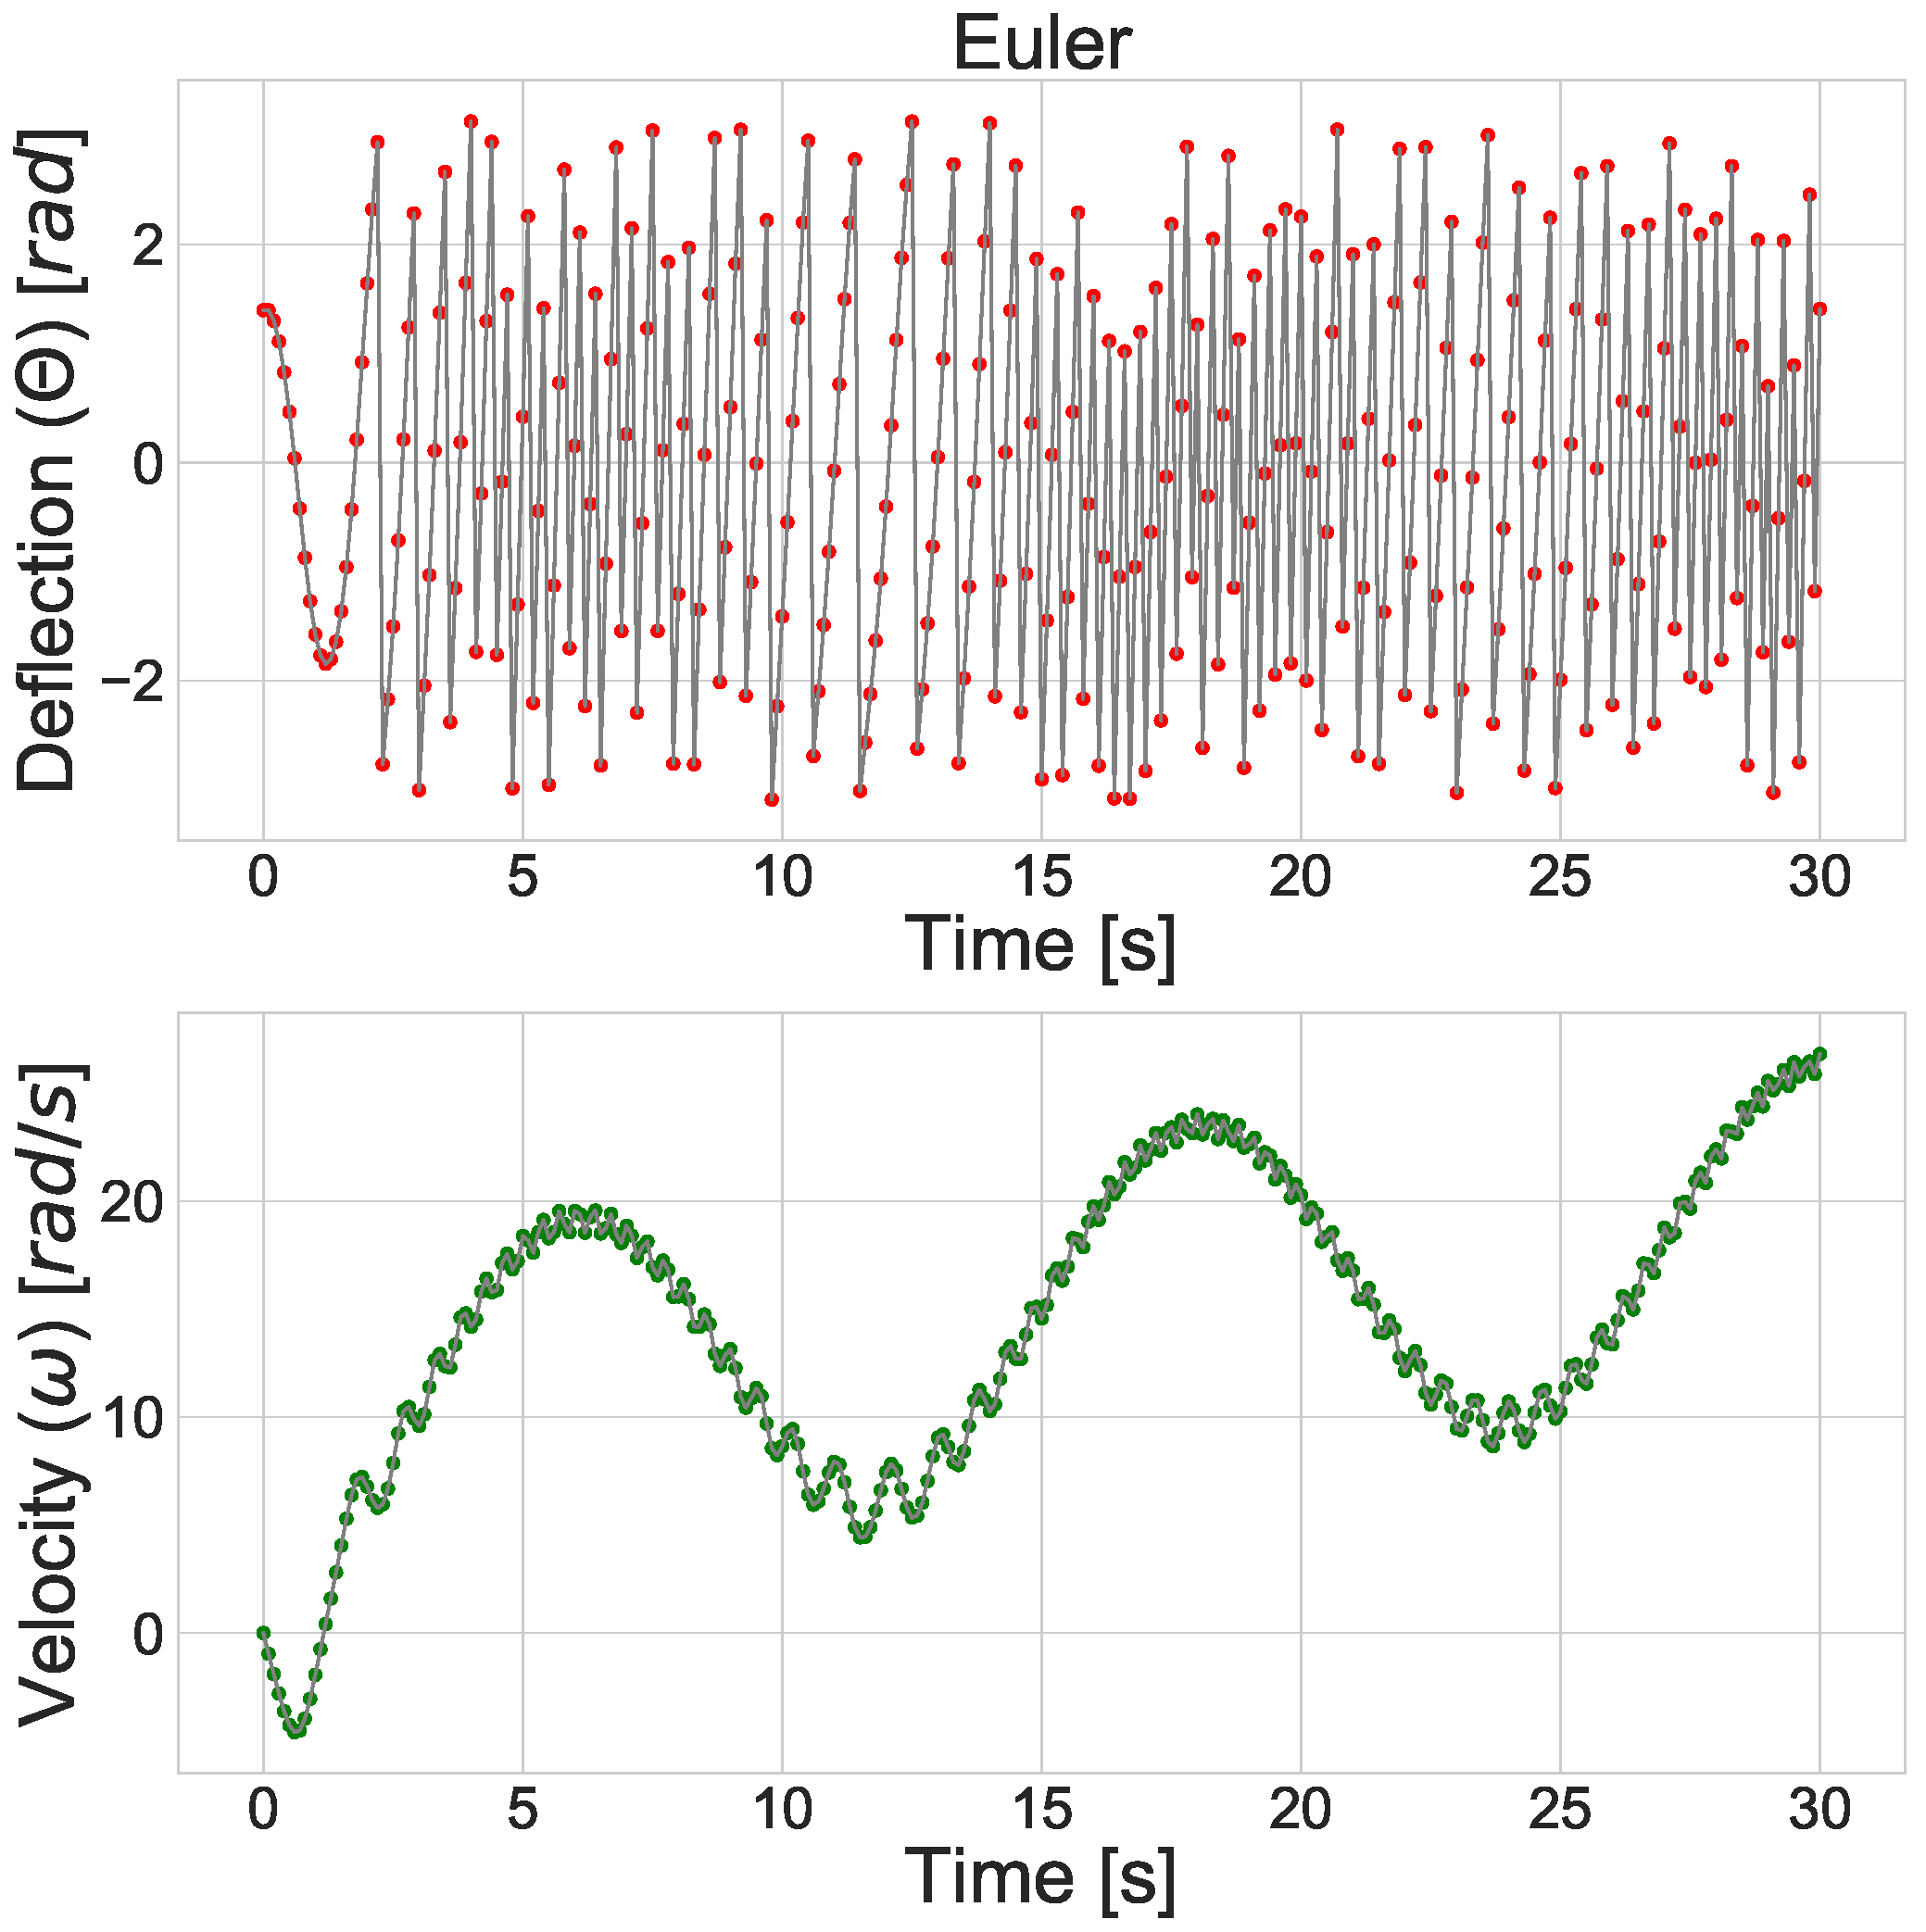
\includegraphics[width=.25\textwidth]{images/theta_omega_euler_driven.pdf}}
\captionof{figure}{Euler\\Driv.}\label{fig:23}
\hfill

\end{multicols}
\begin{multicols}{4}

{\centering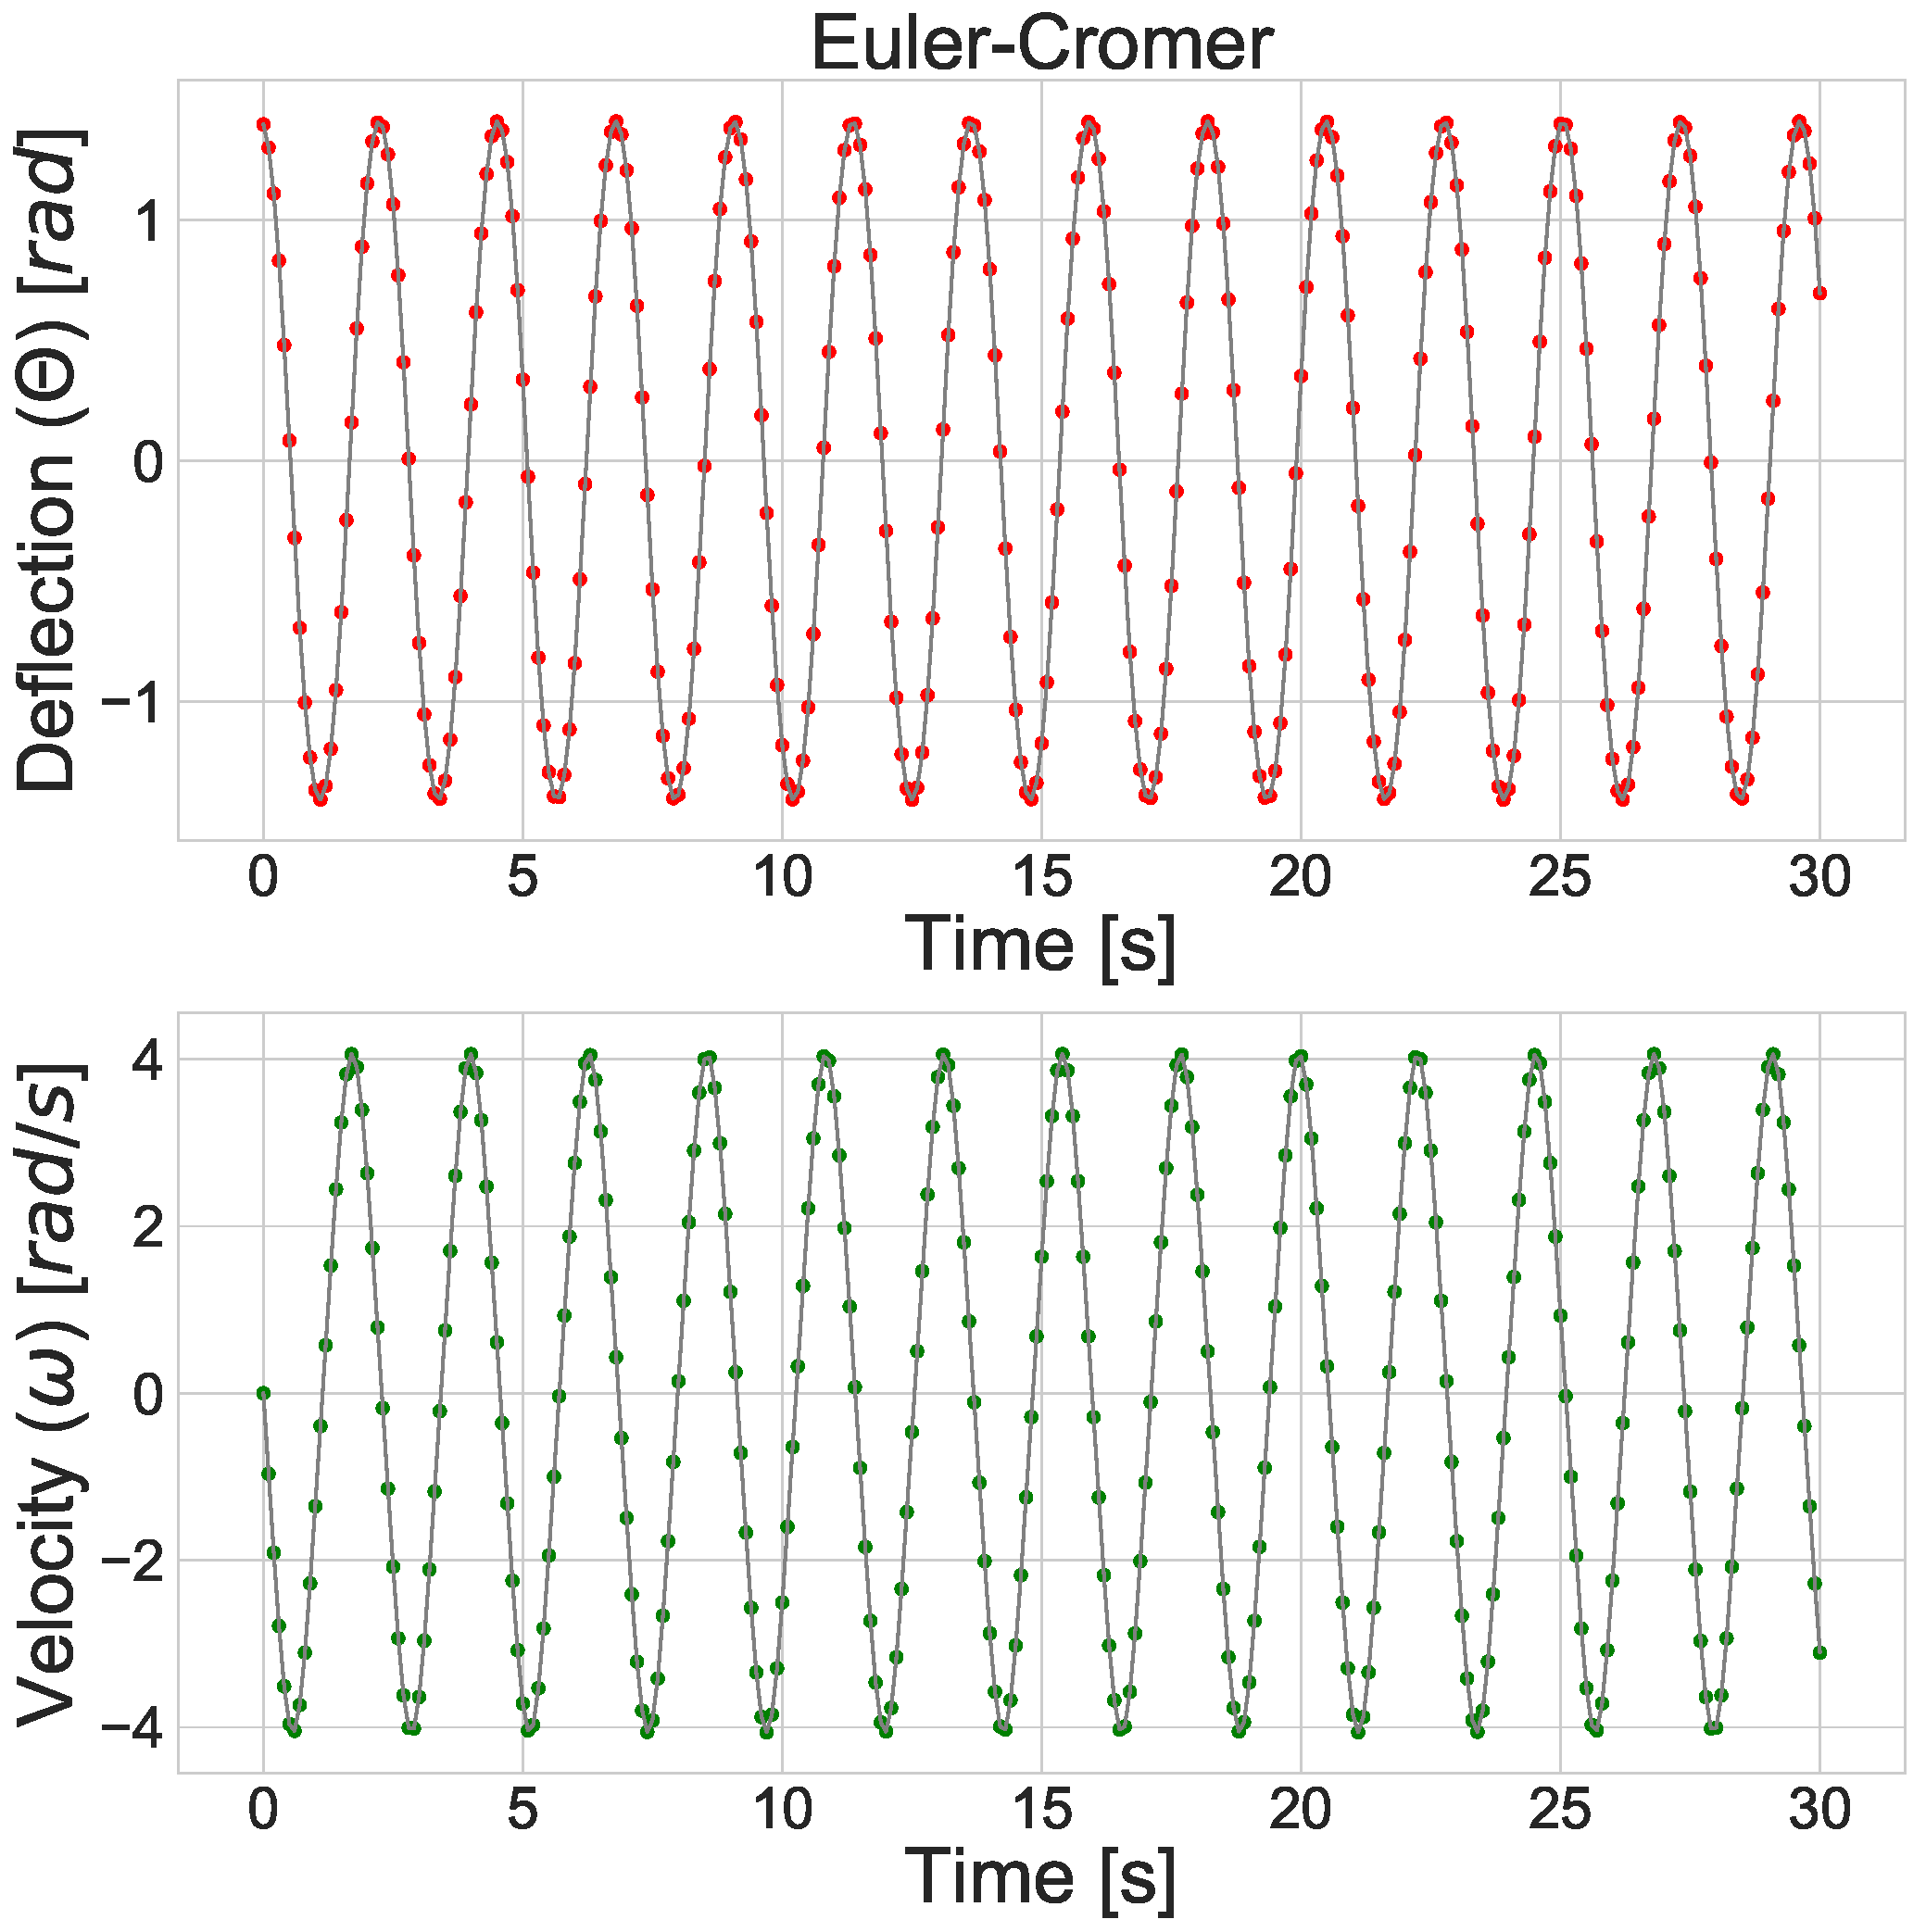
\includegraphics[width=.25\textwidth]{images/theta_omega_eulercromer.pdf}}
\captionof{figure}{Euler-Cromer\\Mat.}\label{fig:24}
\hfill
{\centering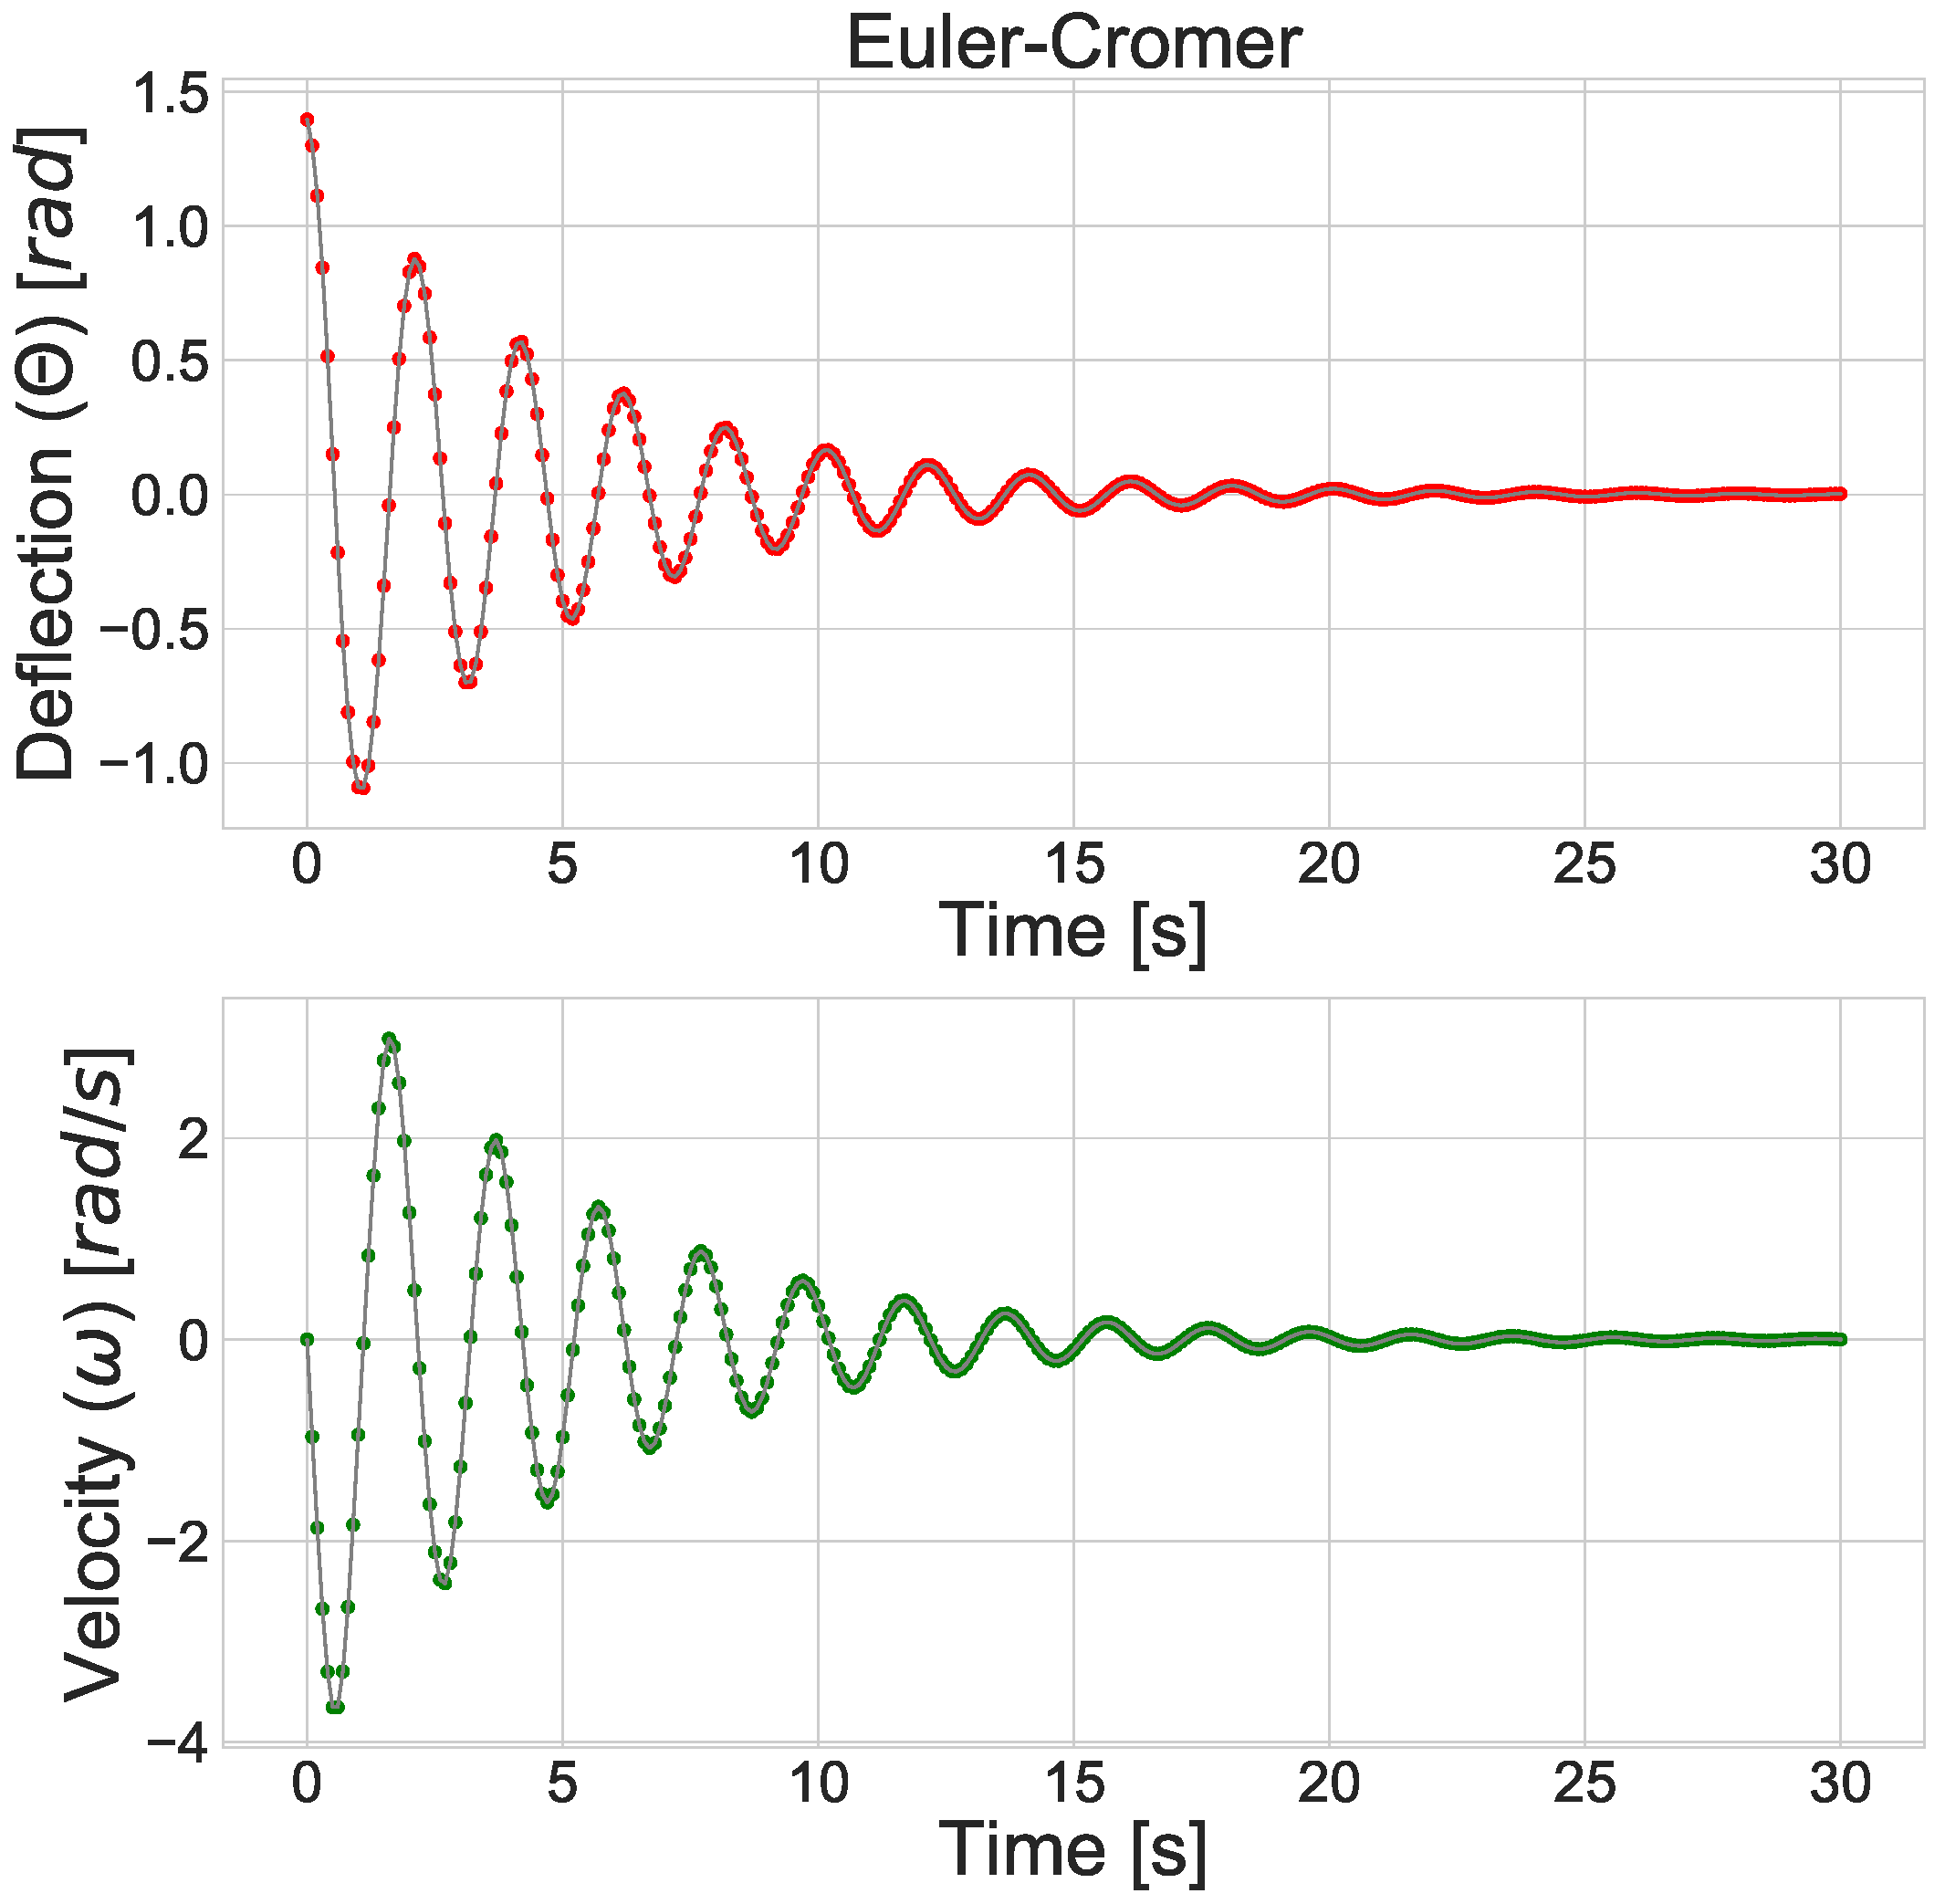
\includegraphics[width=.25\textwidth]{images/theta_omega_eulercromer_damped.pdf}}
\captionof{figure}{Euler-Cromer\\Damp.}\label{fig:25}
\hfill
{\centering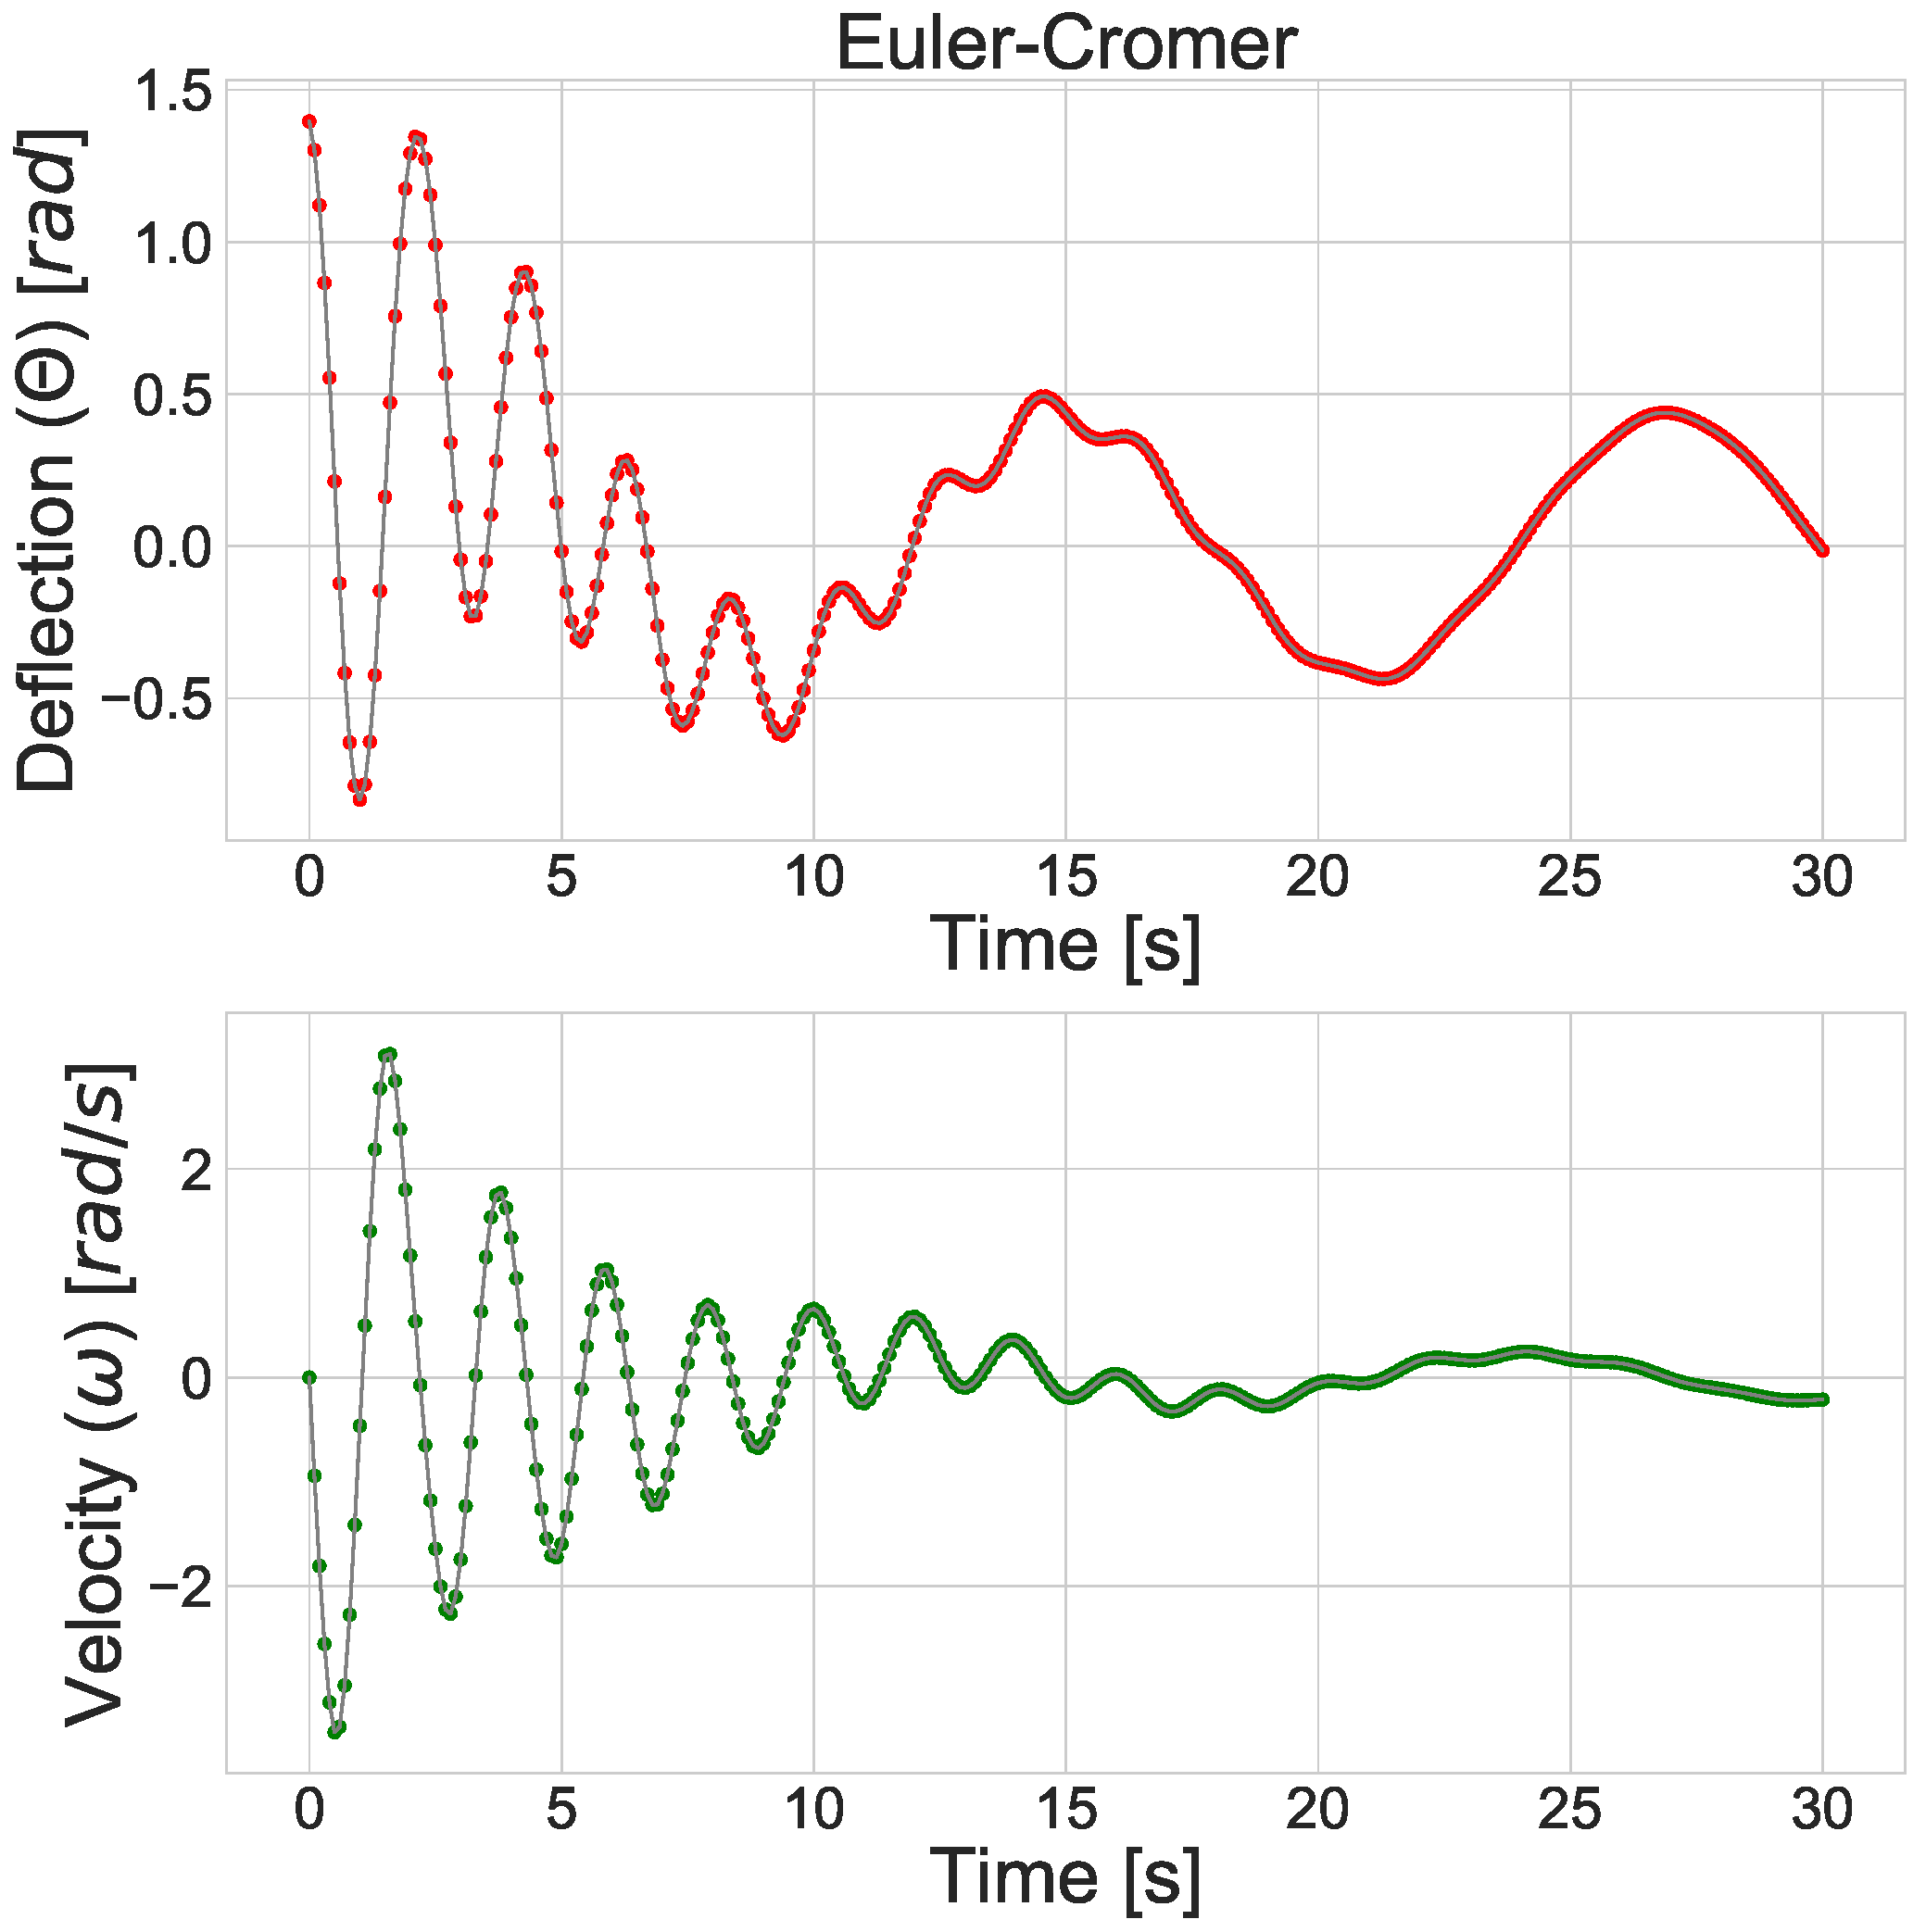
\includegraphics[width=.25\textwidth]{images/theta_omega_eulercromer_dampeddriven.pdf}}
\captionof{figure}{Euler-Cromer\\Damp.-Driv.}\label{fig:26}
\hfill
{\centering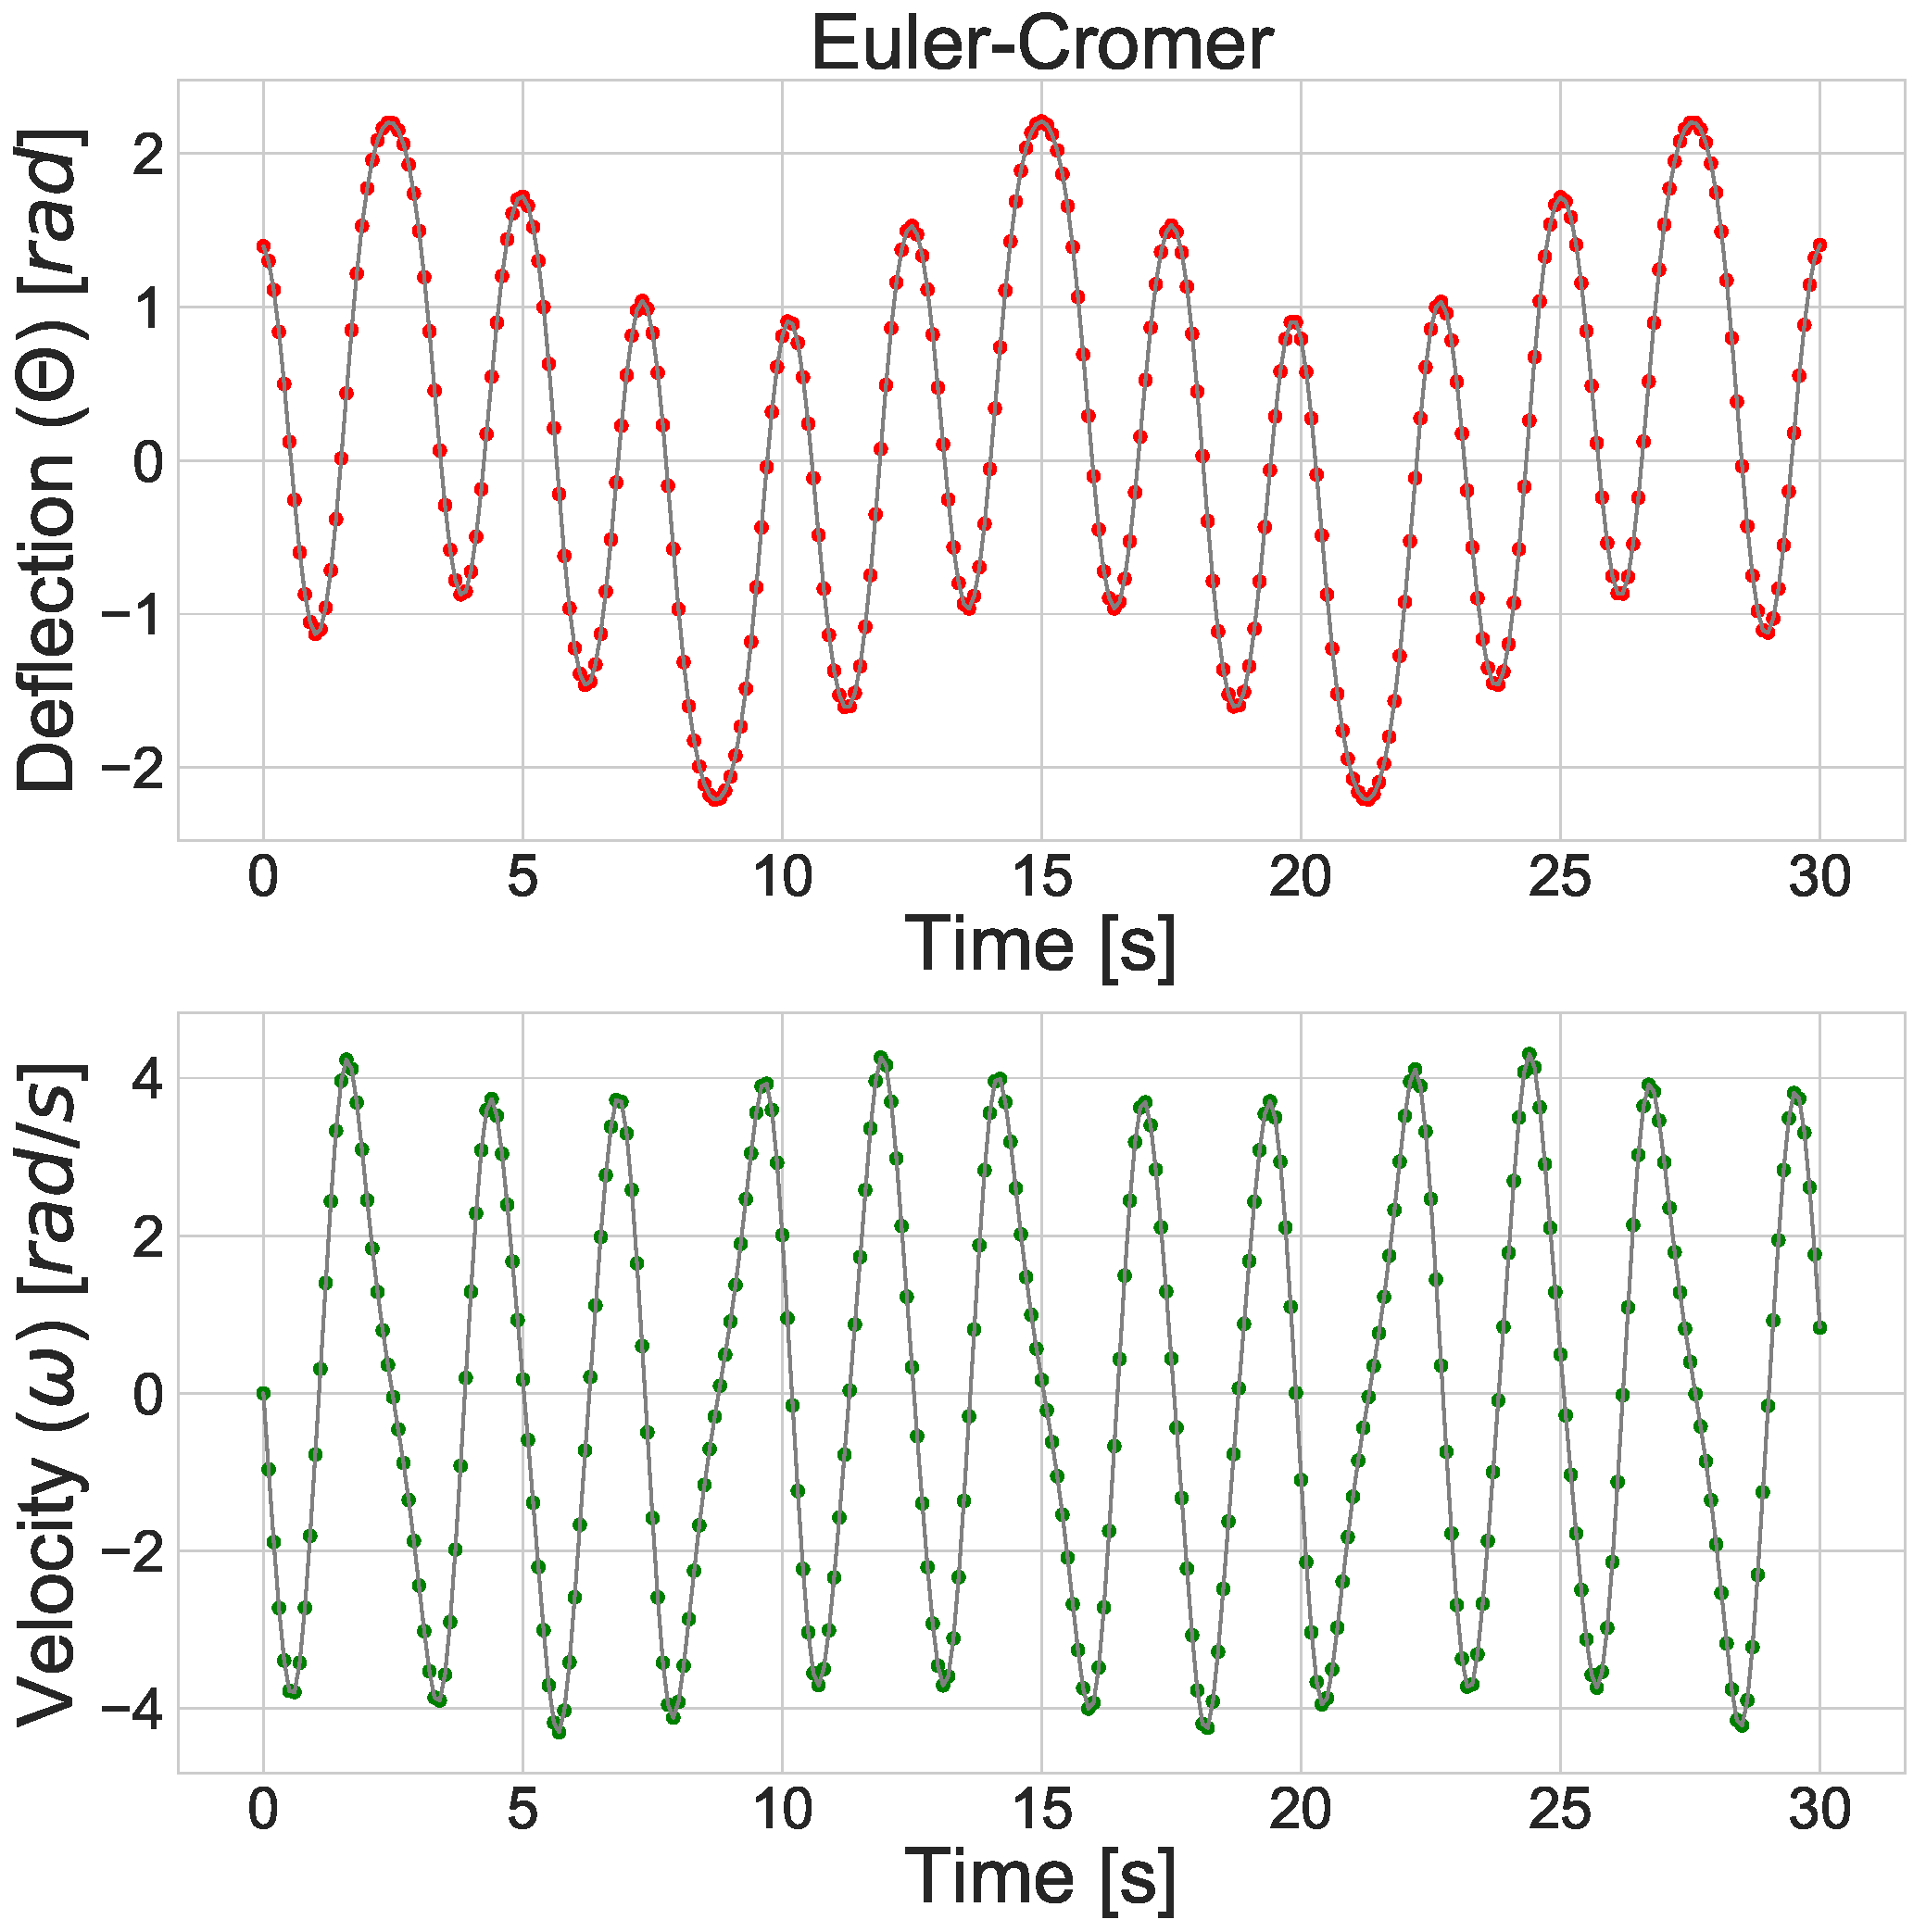
\includegraphics[width=.25\textwidth]{images/theta_omega_eulercromer_driven.pdf}}
\captionof{figure}{Euler-Cromer\\Driv.}\label{fig:27}
\hfill
\end{multicols}

\newpage

\subsubsection*{B.2.\ \ Fázistér és energia-sebesség diagramok, szimpla inga}

\begin{multicols}{4}

{\centering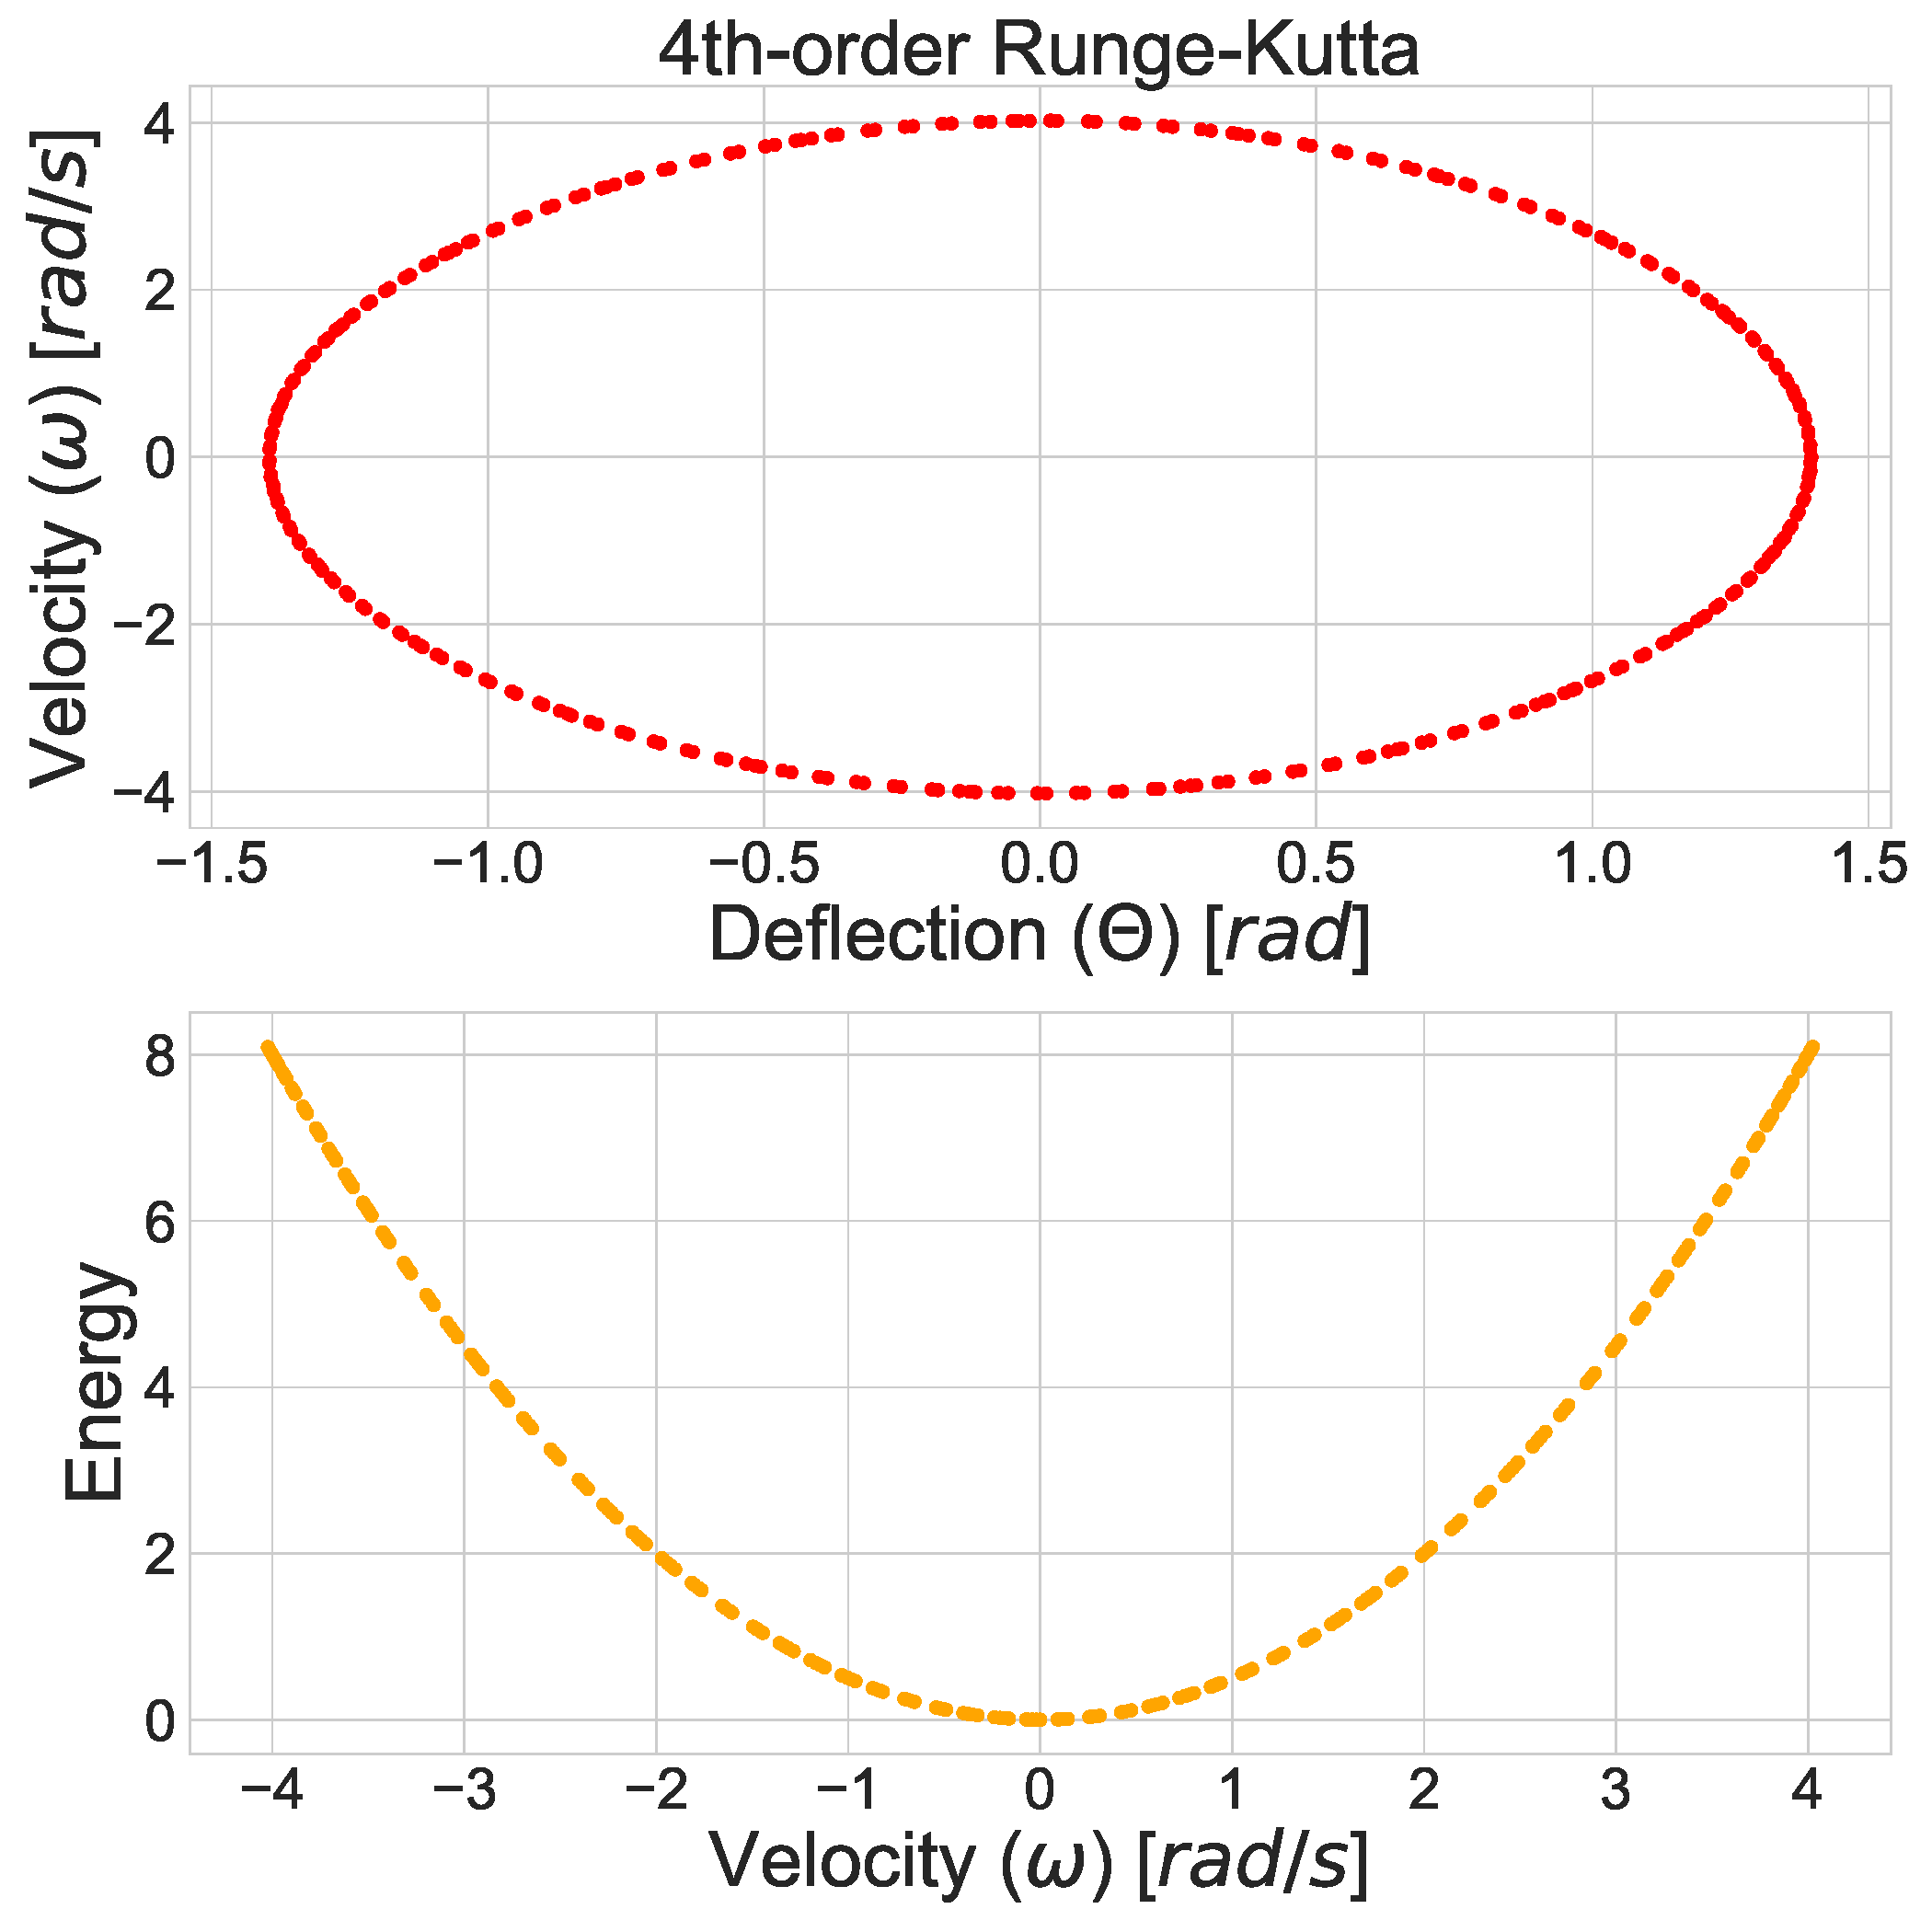
\includegraphics[width=.25\textwidth]{images/phase_energy_runge.pdf}}
\captionof{figure}{Runge-Kutta\\Mat.}\label{fig:28}
\hfill
{\centering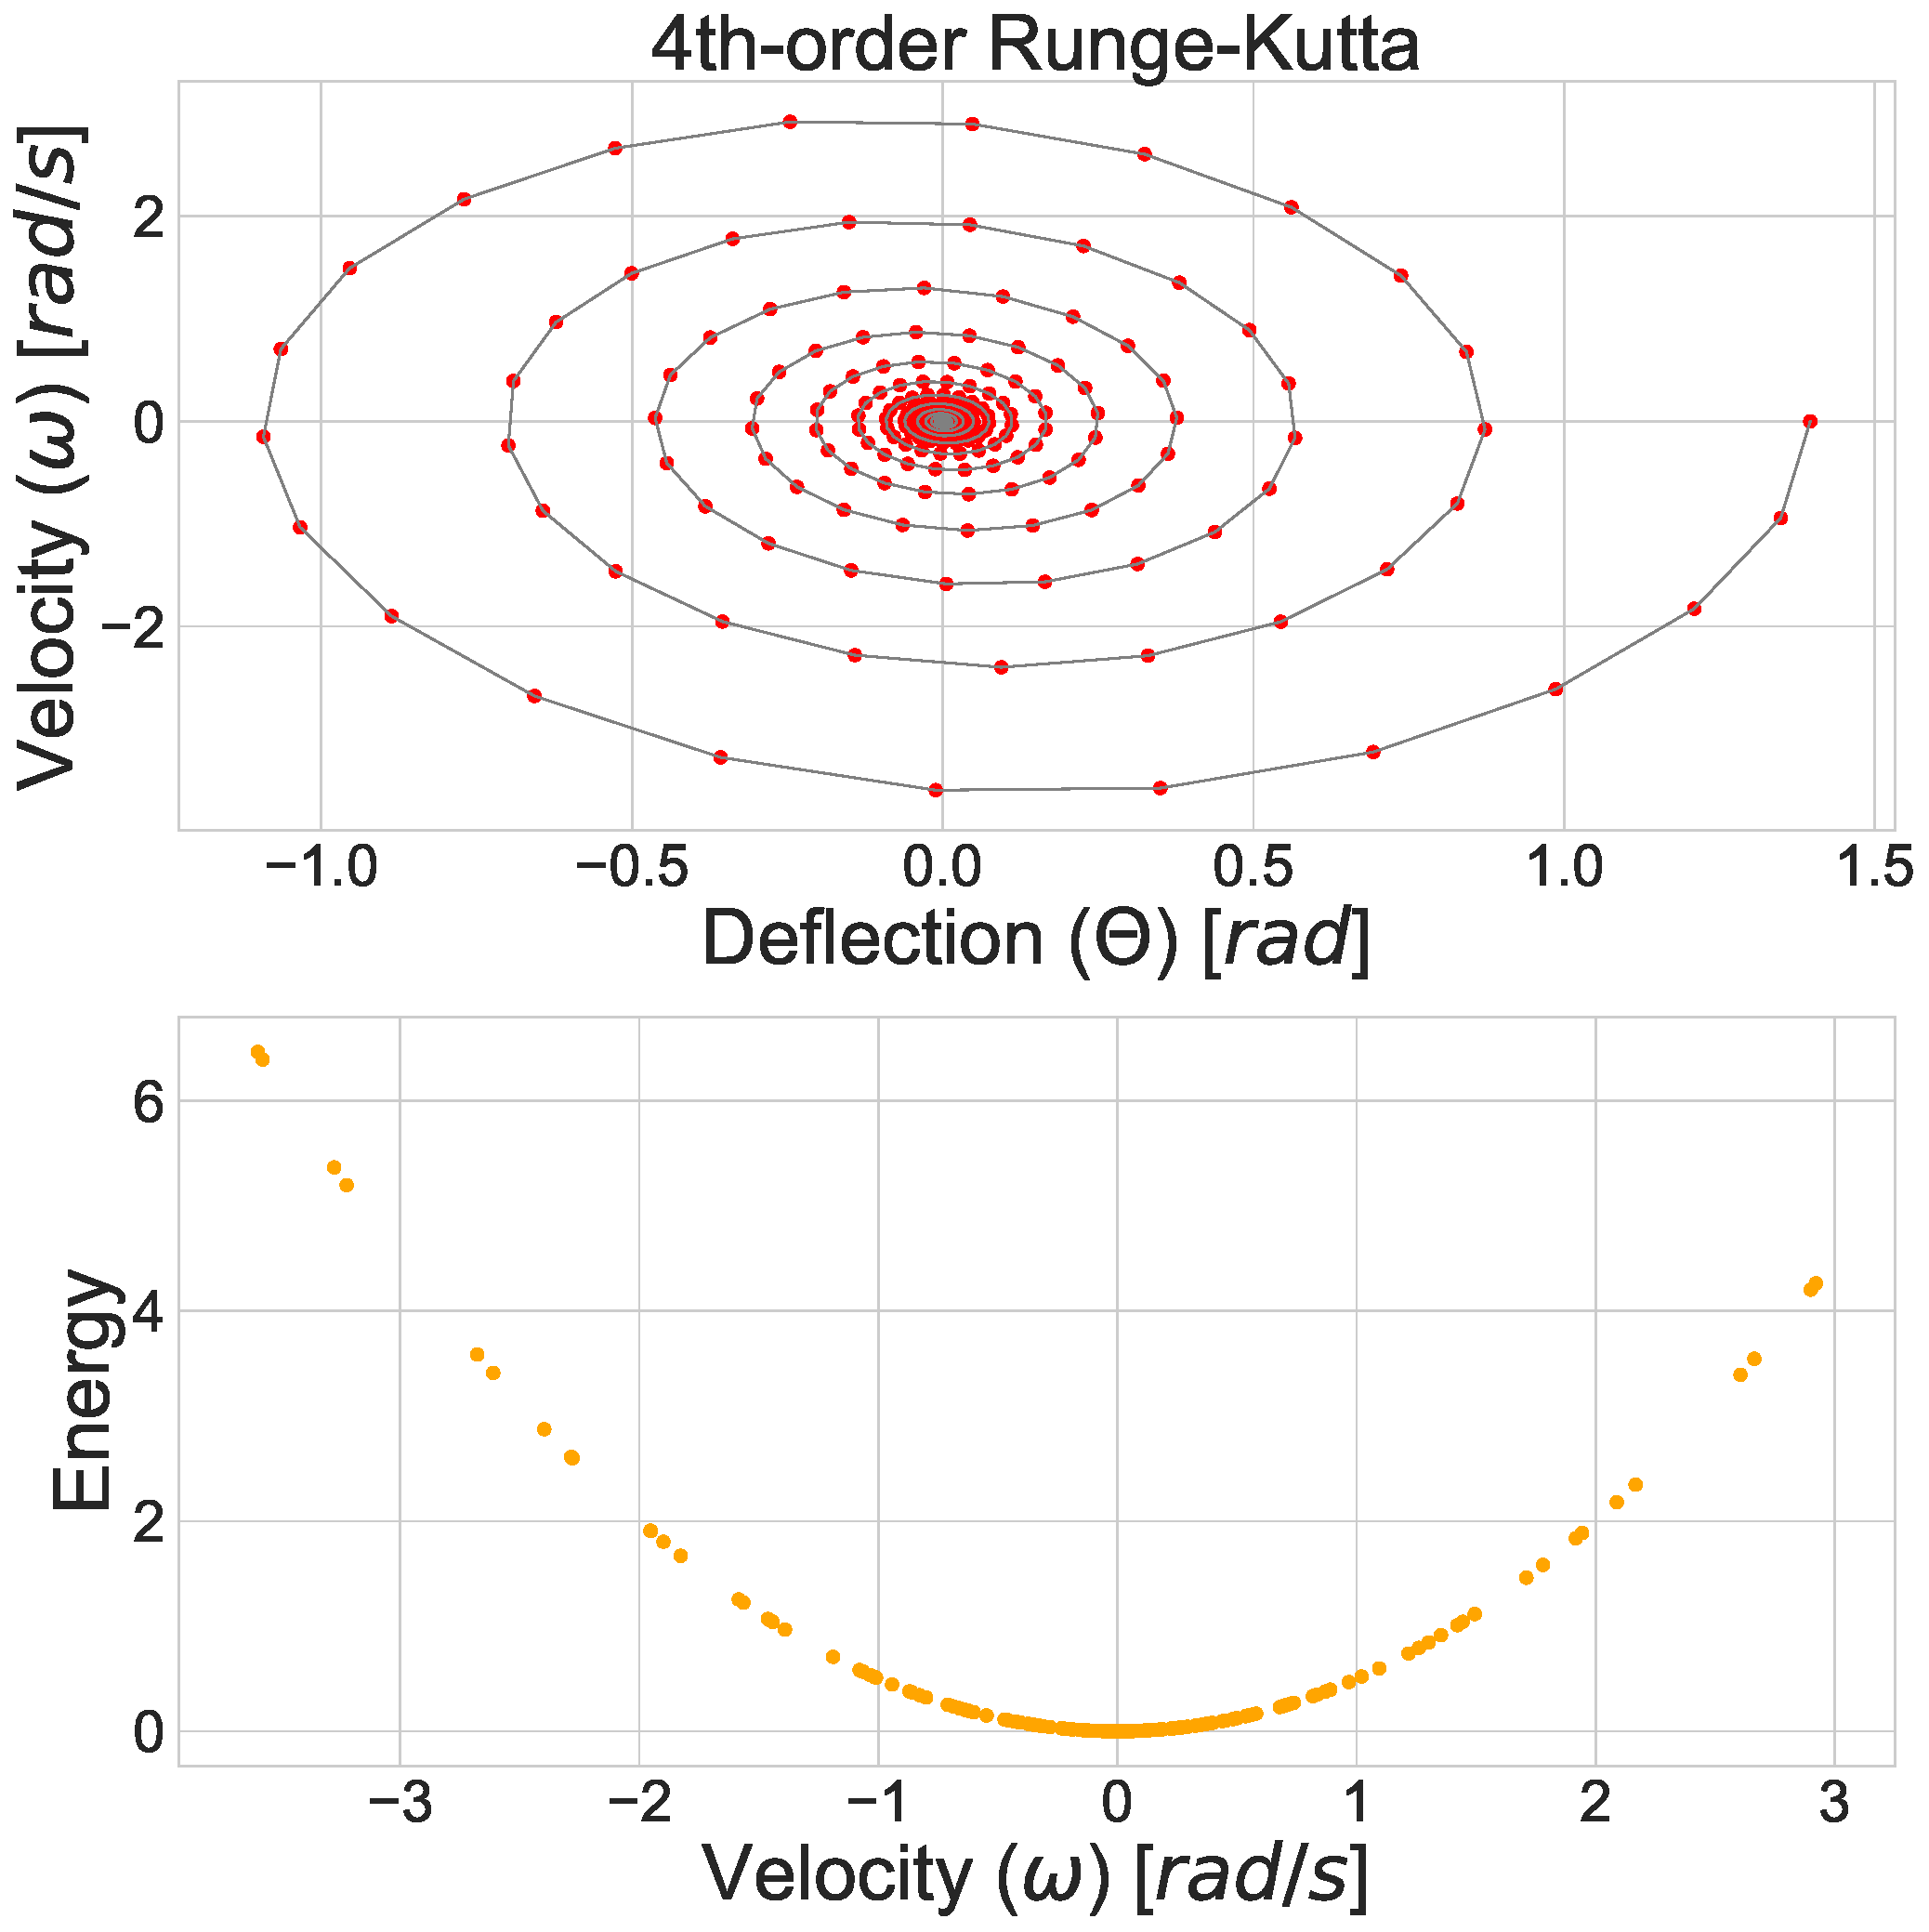
\includegraphics[width=.25\textwidth]{images/phase_energy_runge_damped.pdf}}
\captionof{figure}{Runge-Kutta\\Damp.}\label{fig:29}
\hfill
{\centering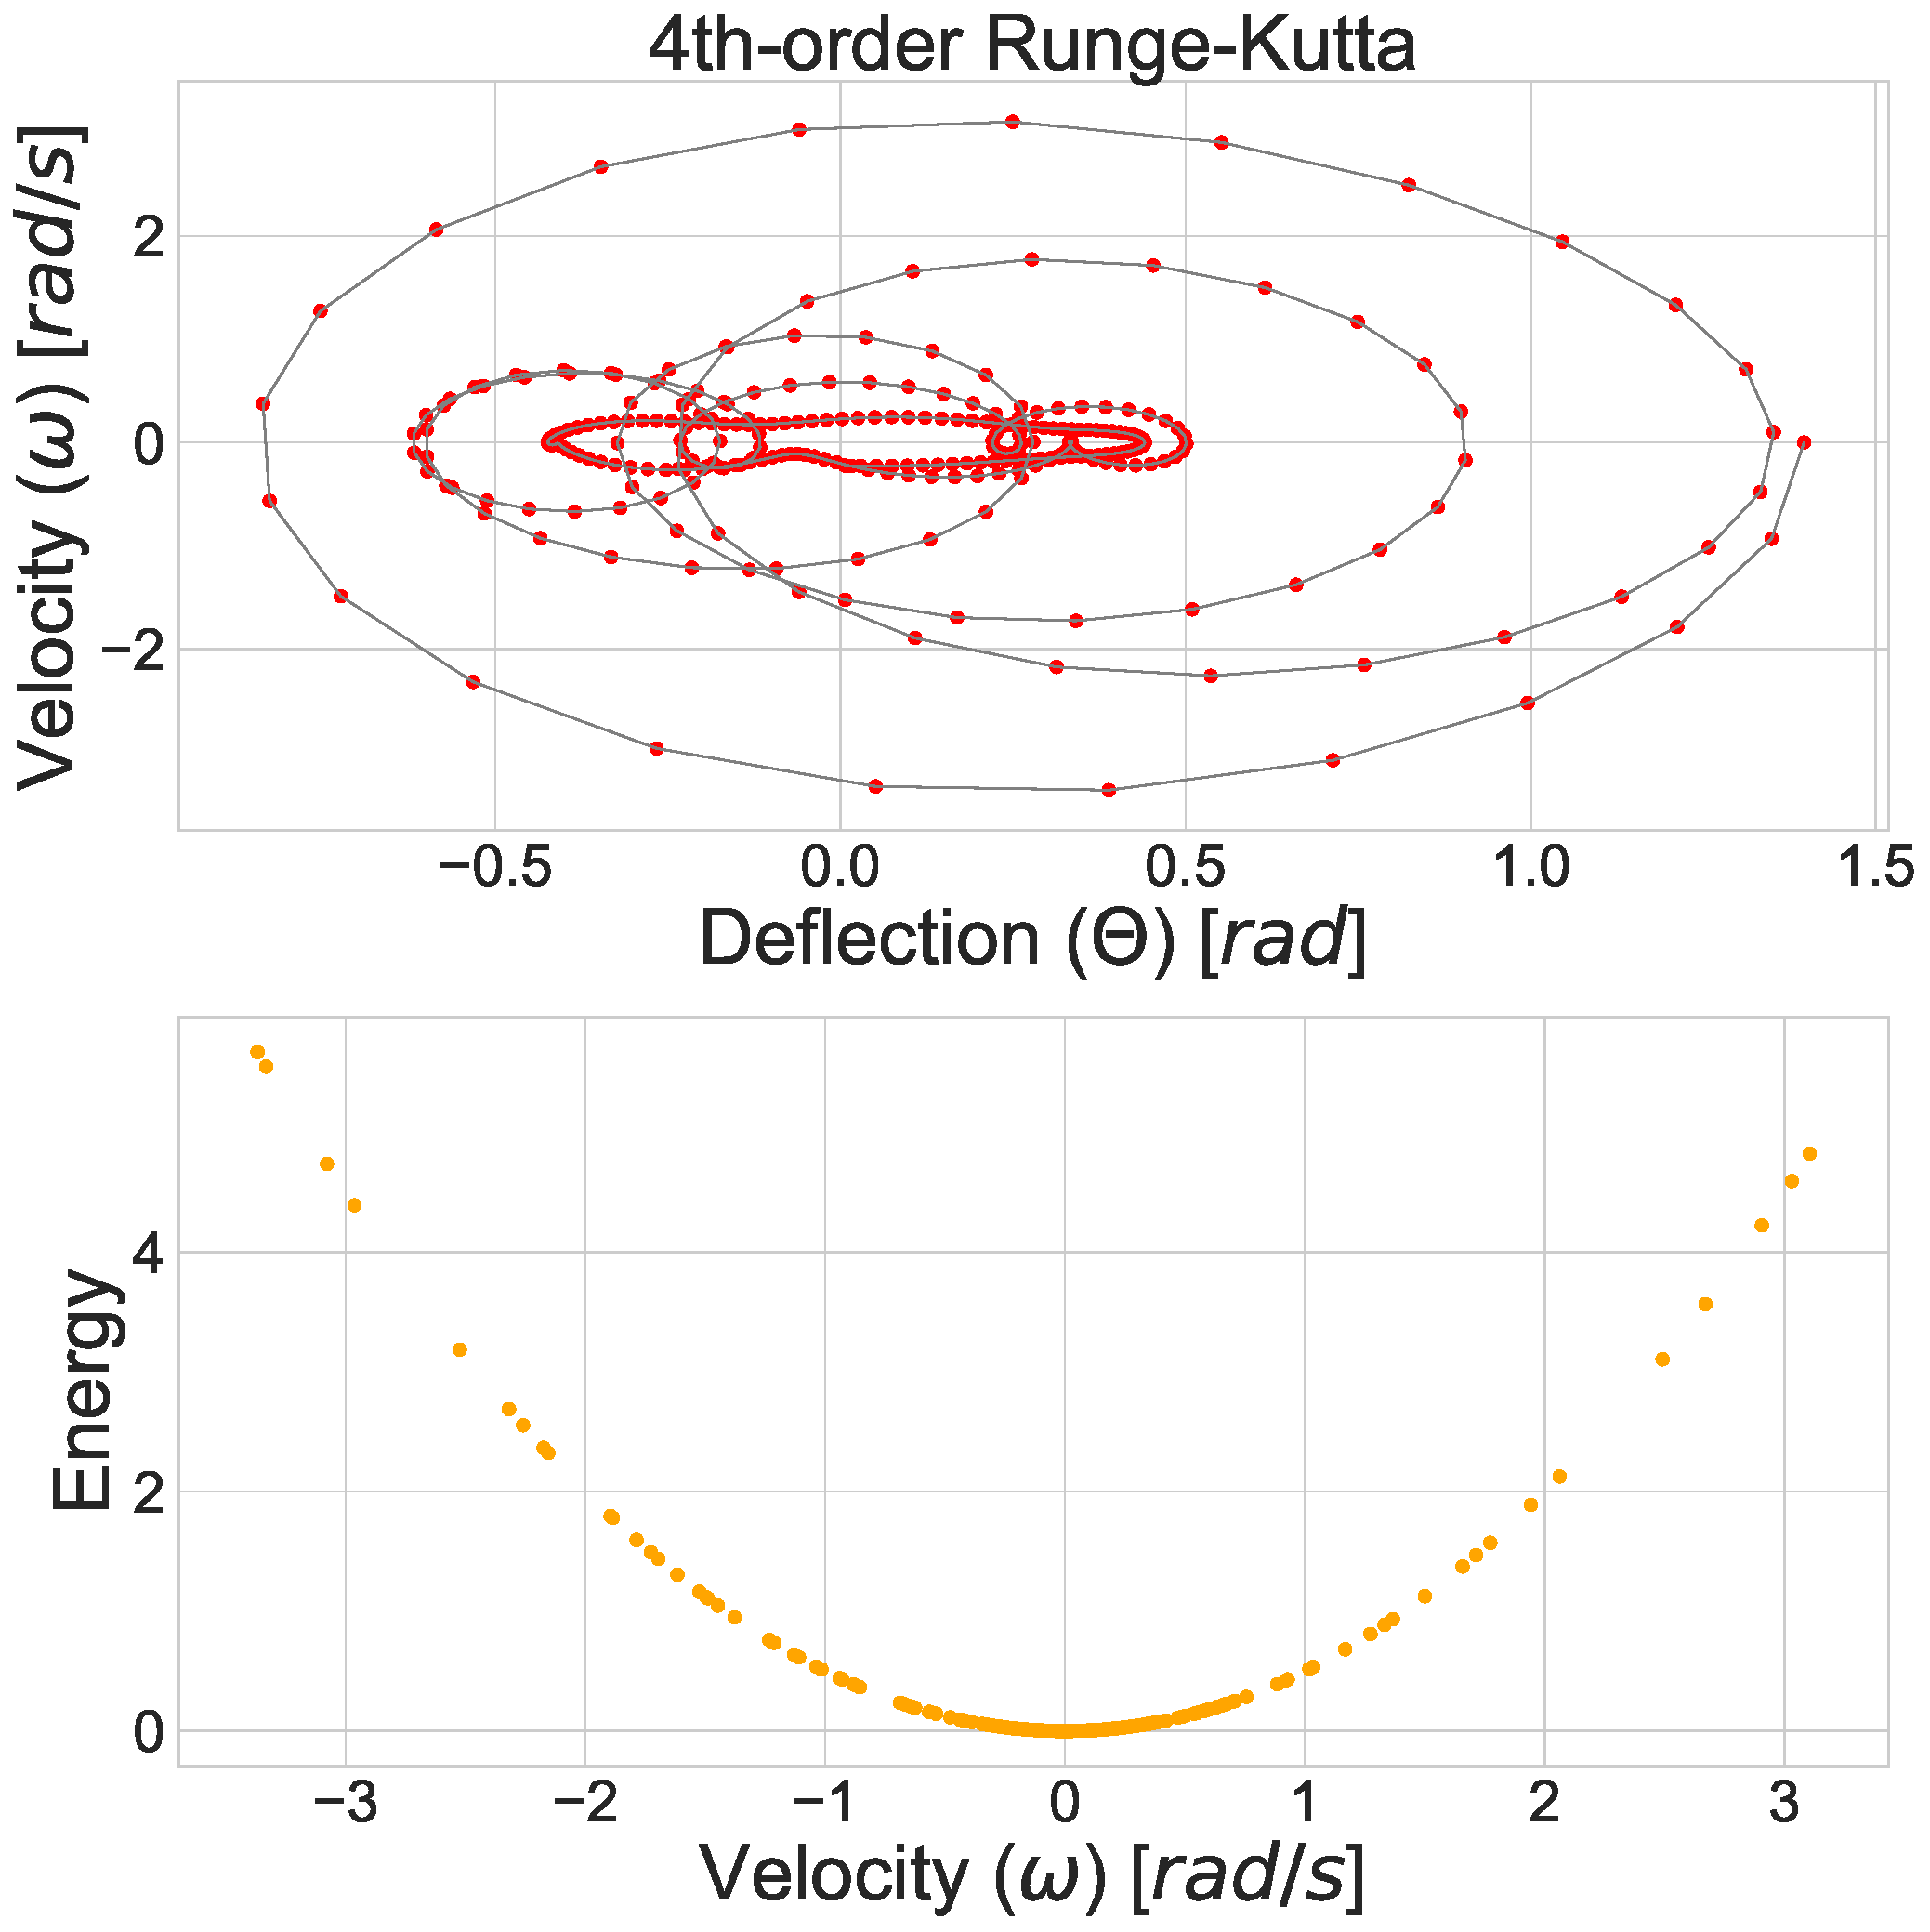
\includegraphics[width=.25\textwidth]{images/phase_energy_runge_dampeddriven.pdf}}
\captionof{figure}{Runge-Kutta\\Damp.-Driv.}\label{fig:30}
\hfill
{\centering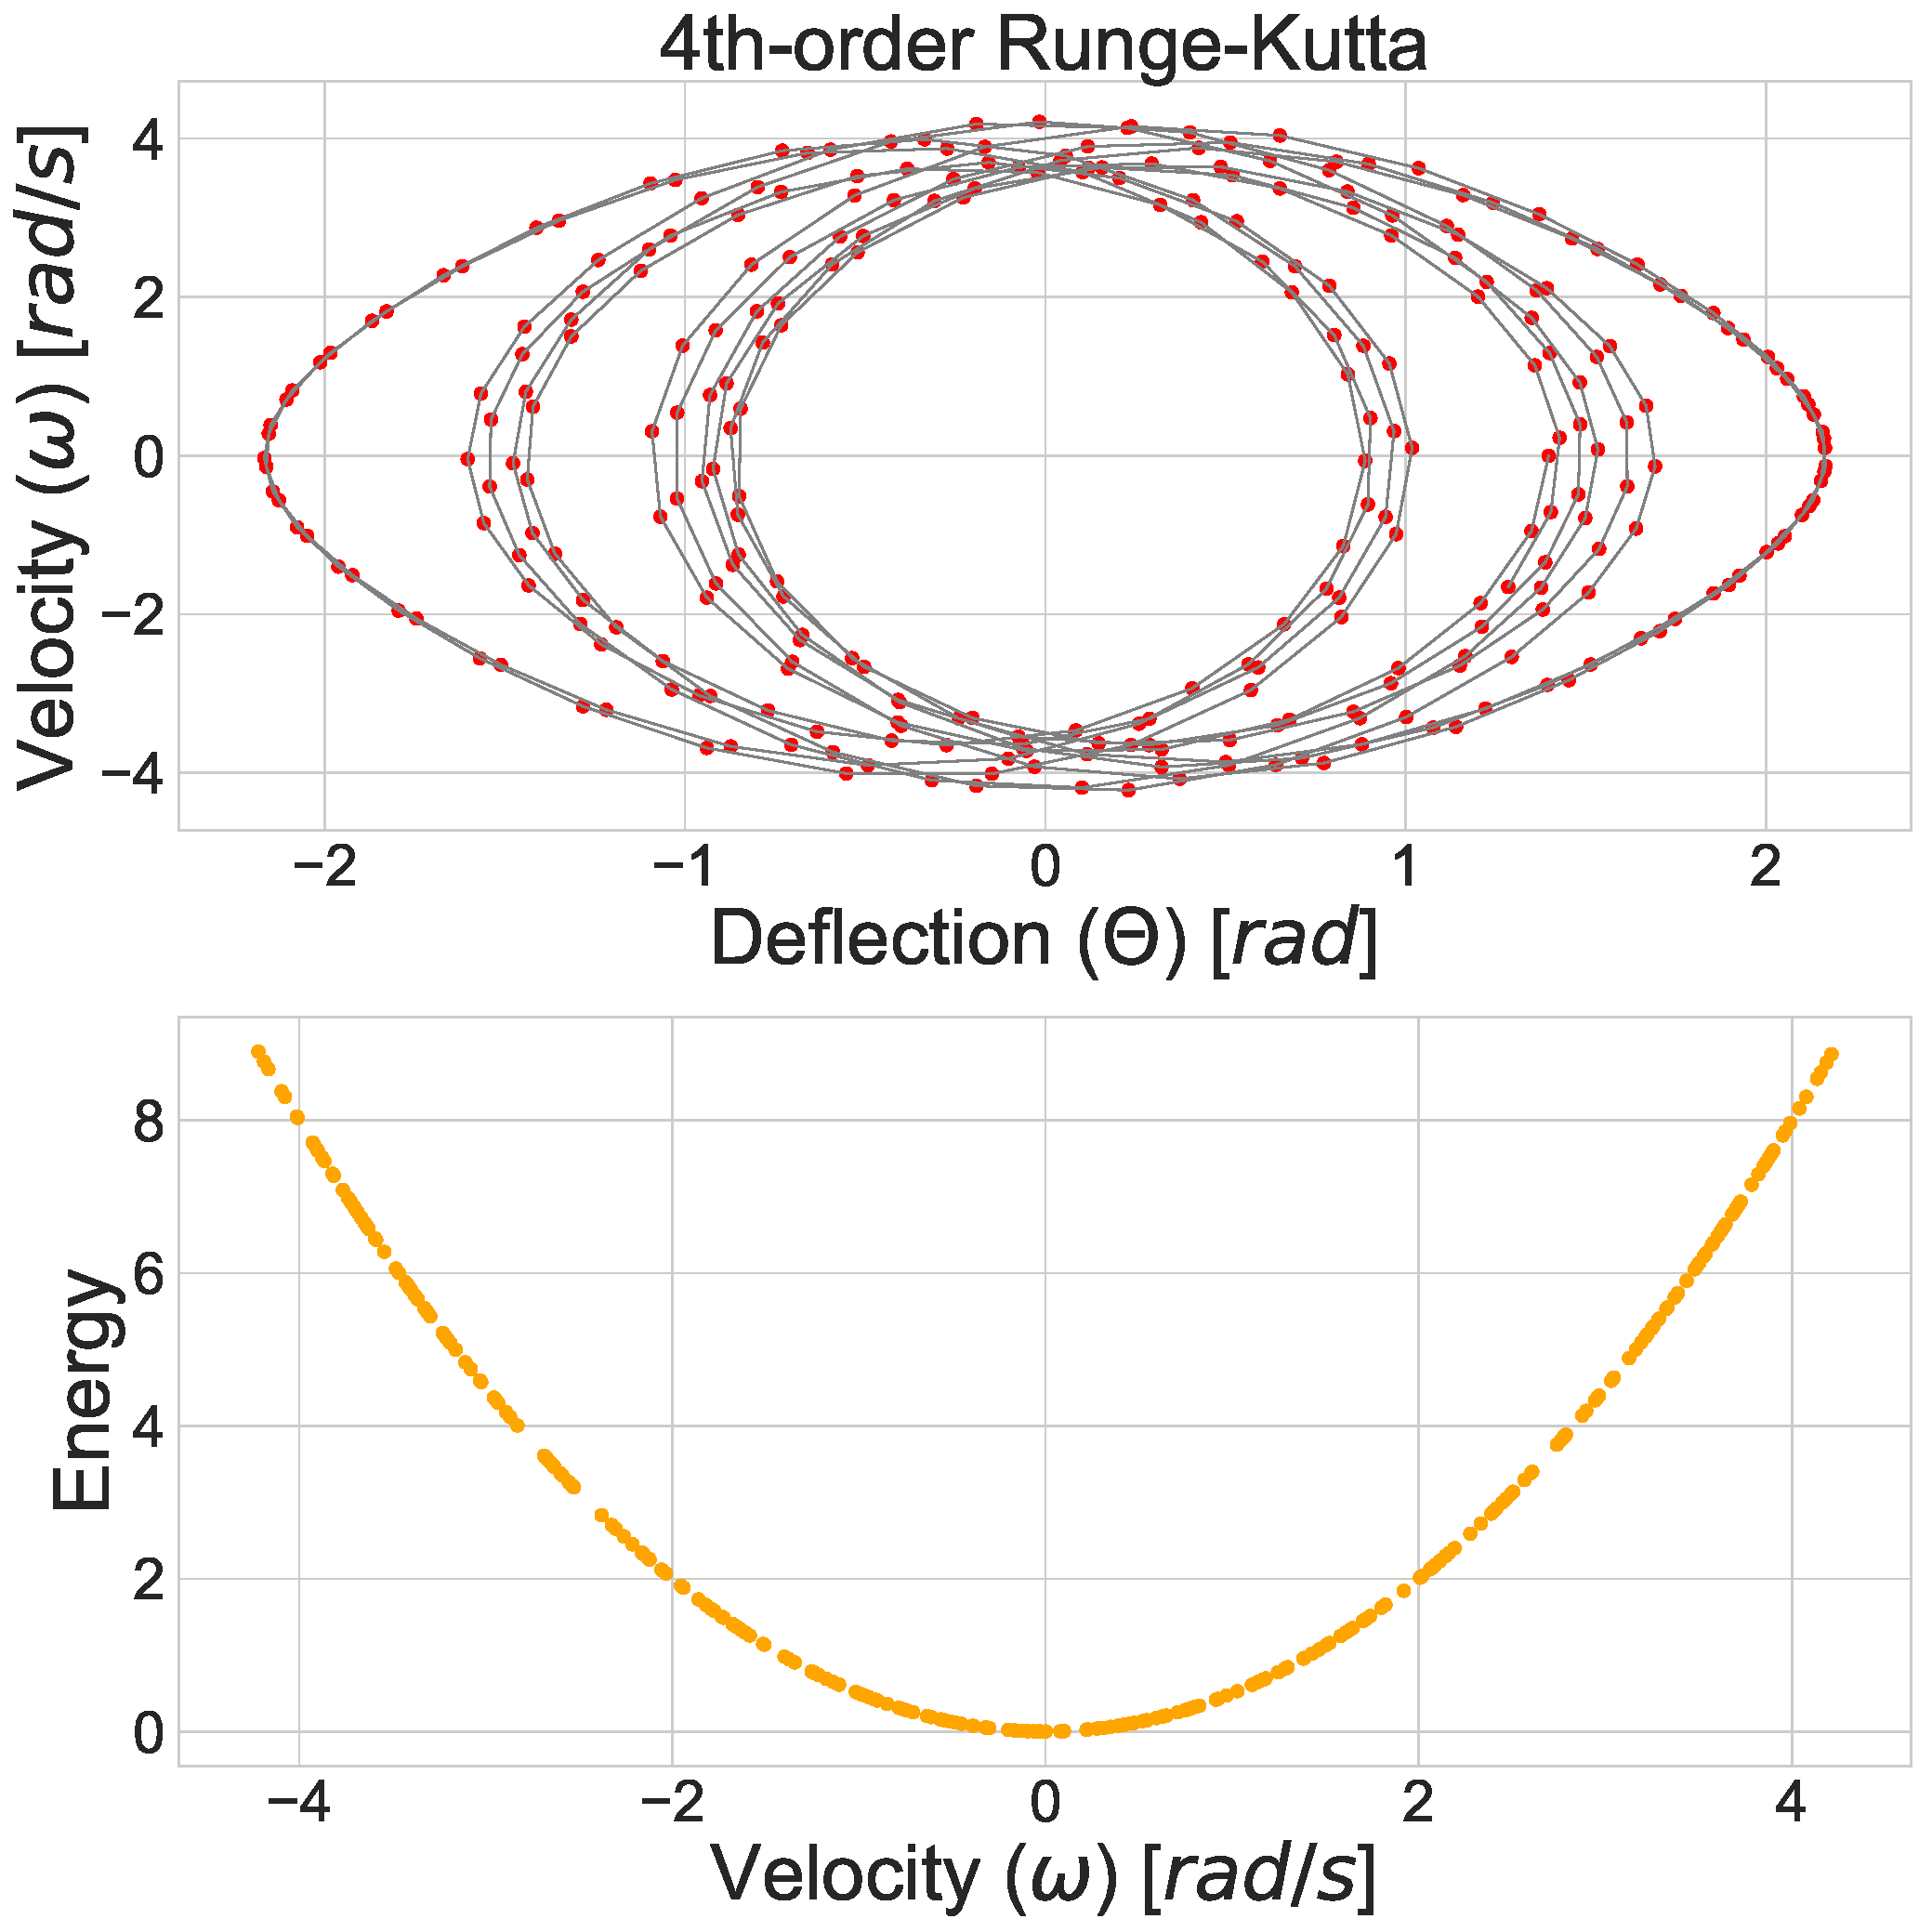
\includegraphics[width=.25\textwidth]{images/phase_energy_runge_driven.pdf}}
\captionof{figure}{Runge-Kutta\\Driv.}\label{fig:31}
\hfill

\end{multicols}
\begin{multicols}{4}

{\centering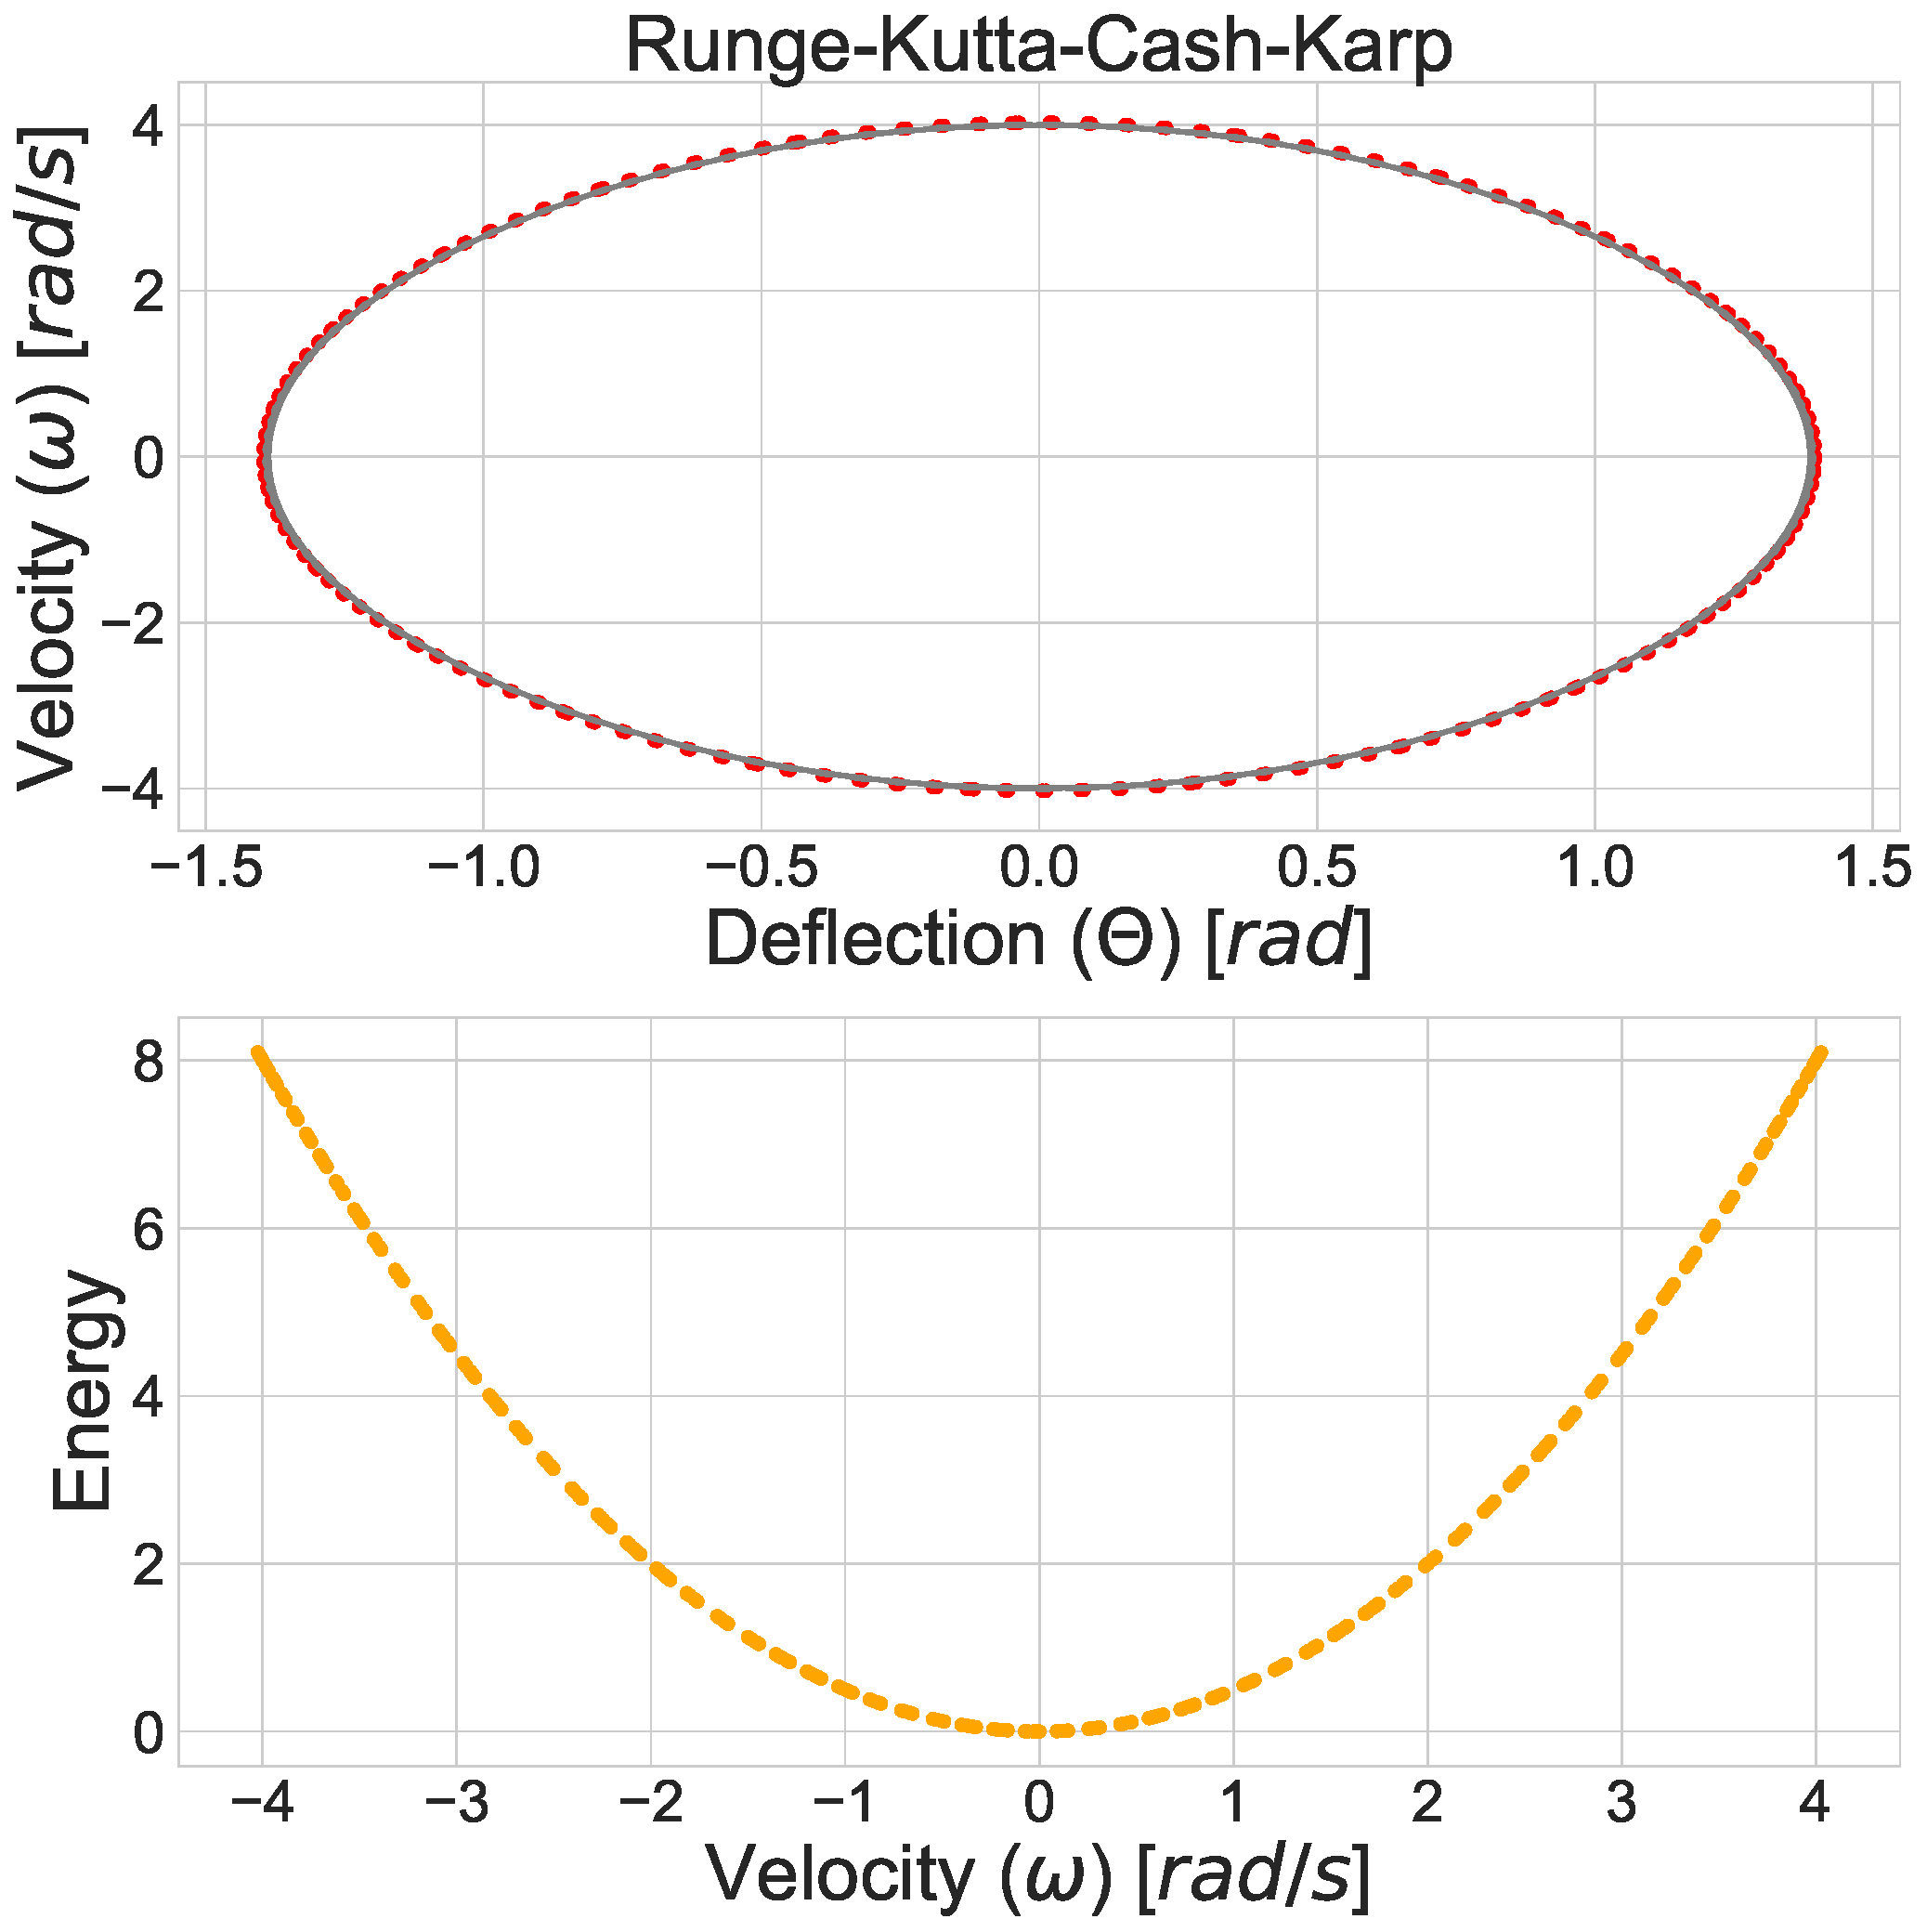
\includegraphics[width=.25\textwidth]{images/phase_energy_rkck.pdf}}
\captionof{figure}{R-K-C-K\\Mat.}\label{fig:32}
\hfill
{\centering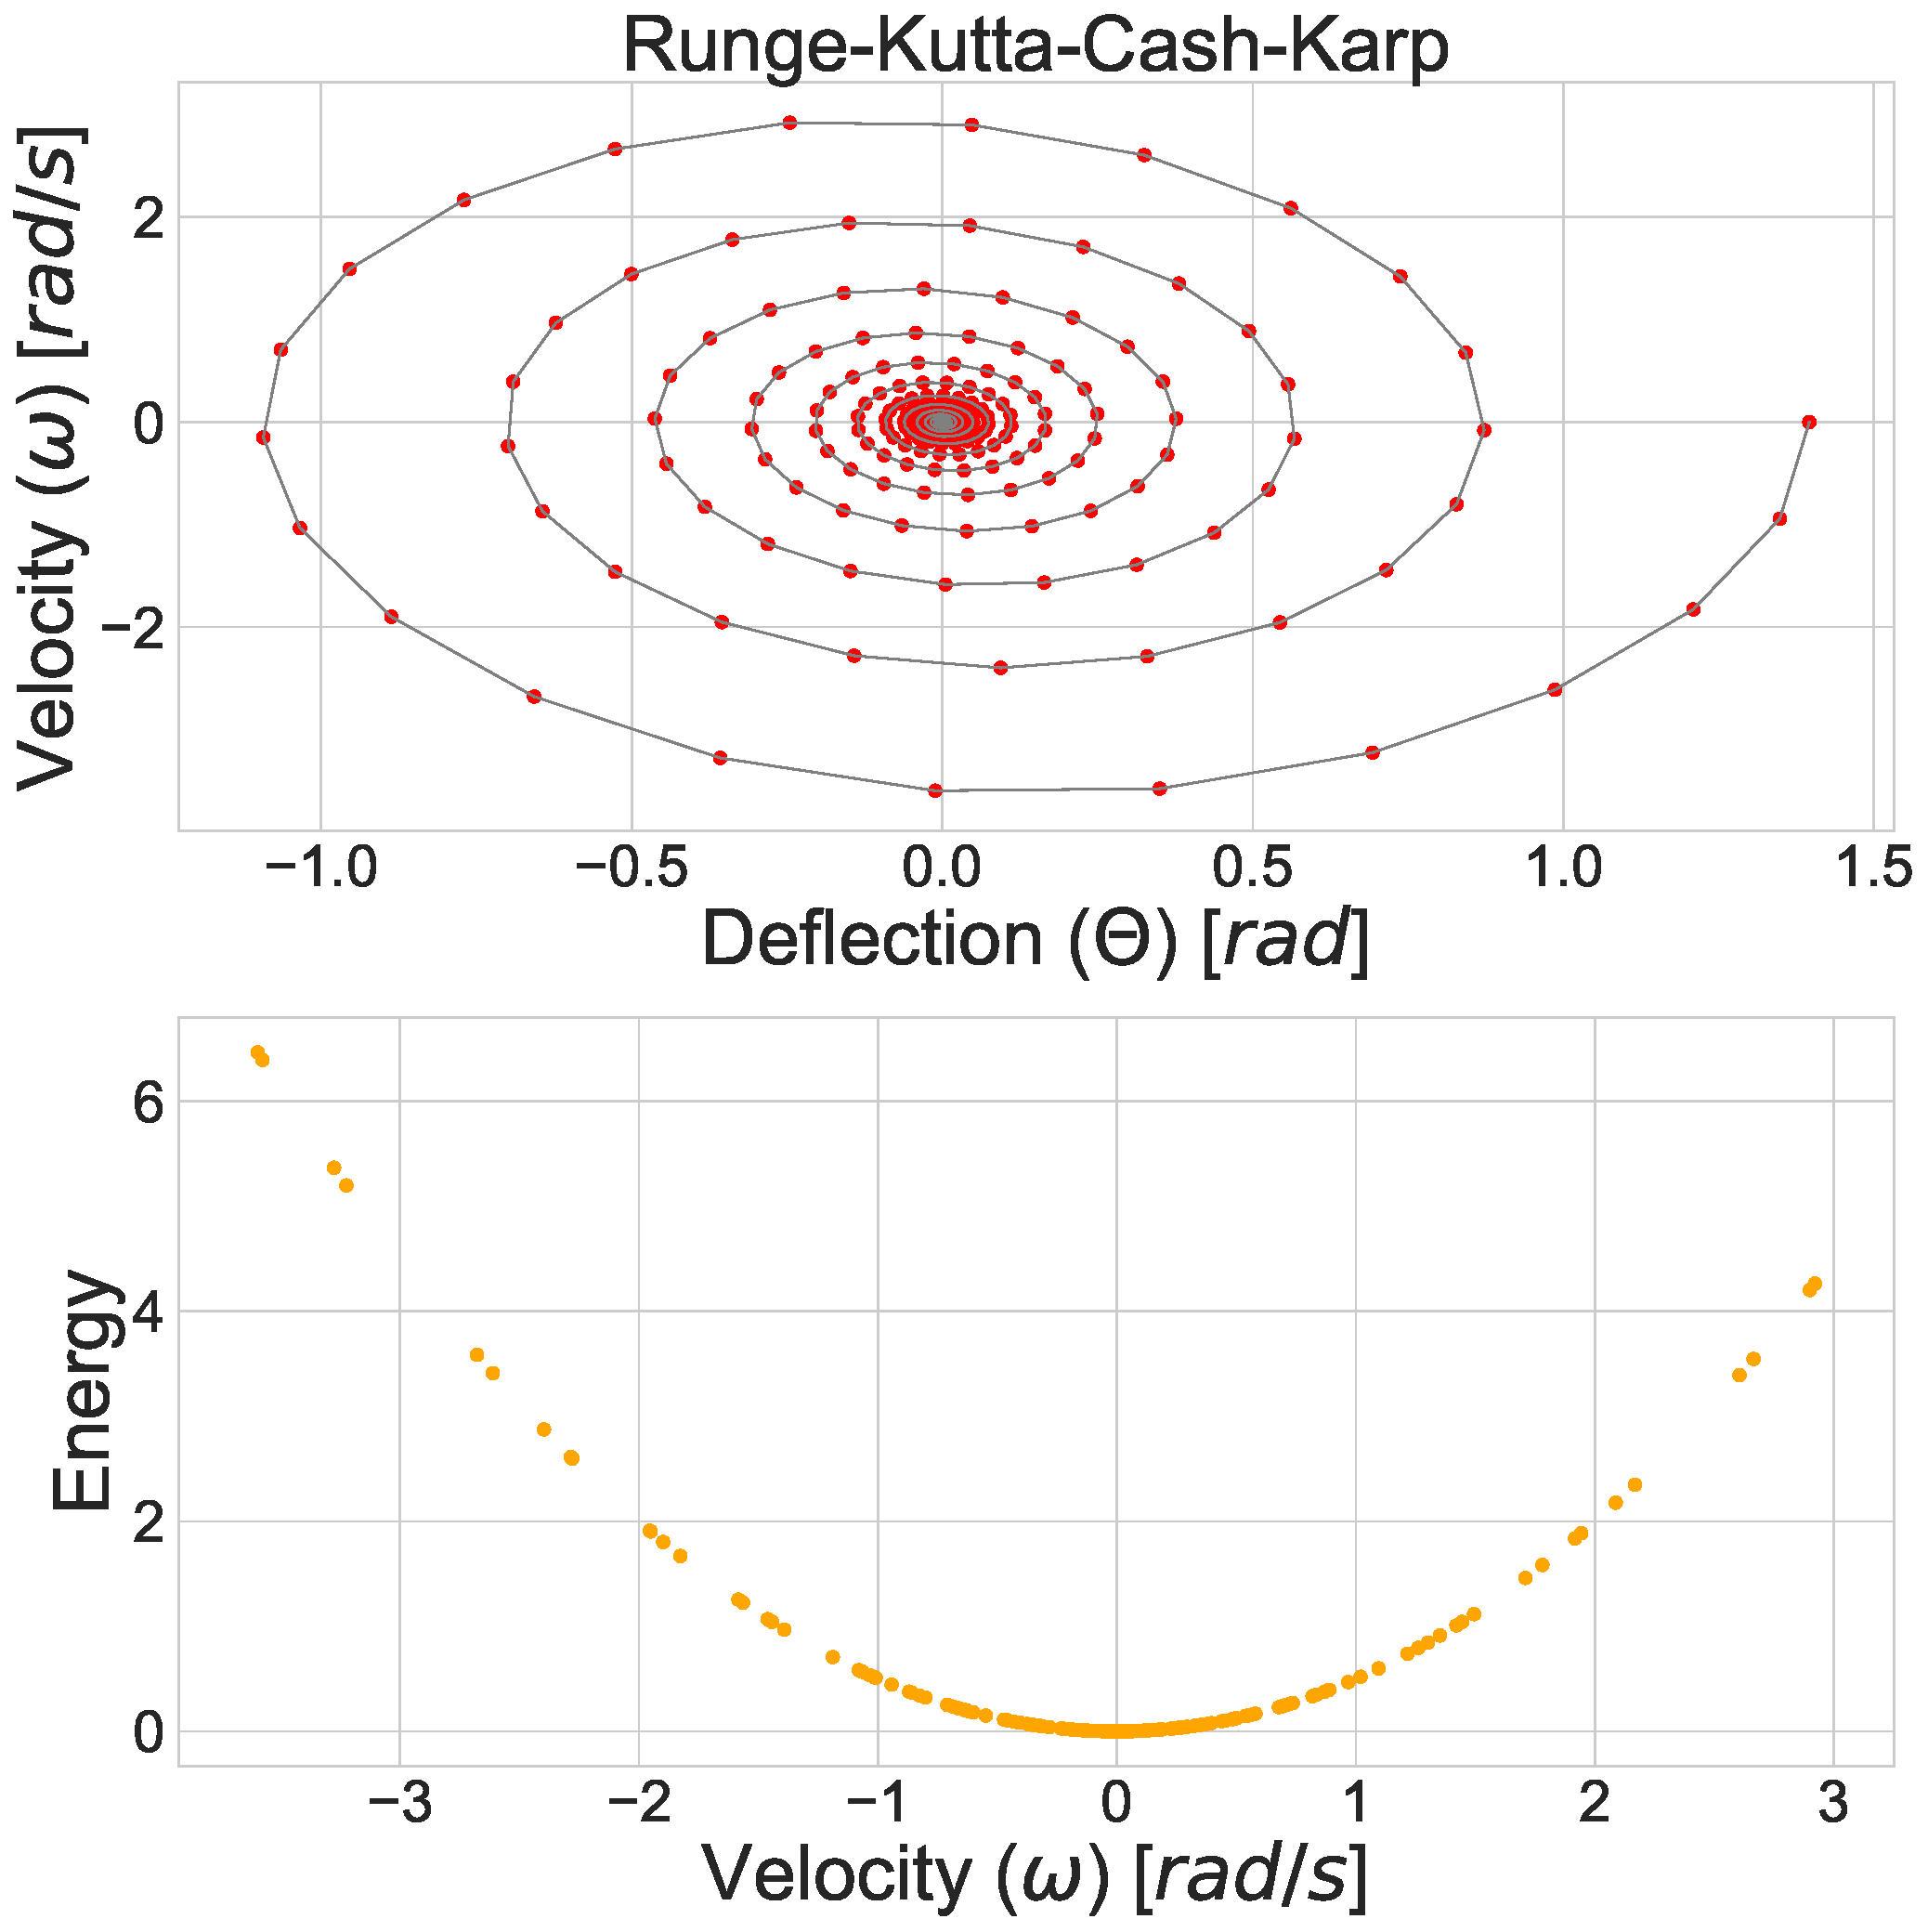
\includegraphics[width=.25\textwidth]{images/phase_energy_rkck_damped.pdf}}
\captionof{figure}{R-K-C-K\\Damp.}\label{fig:33}
\hfill
{\centering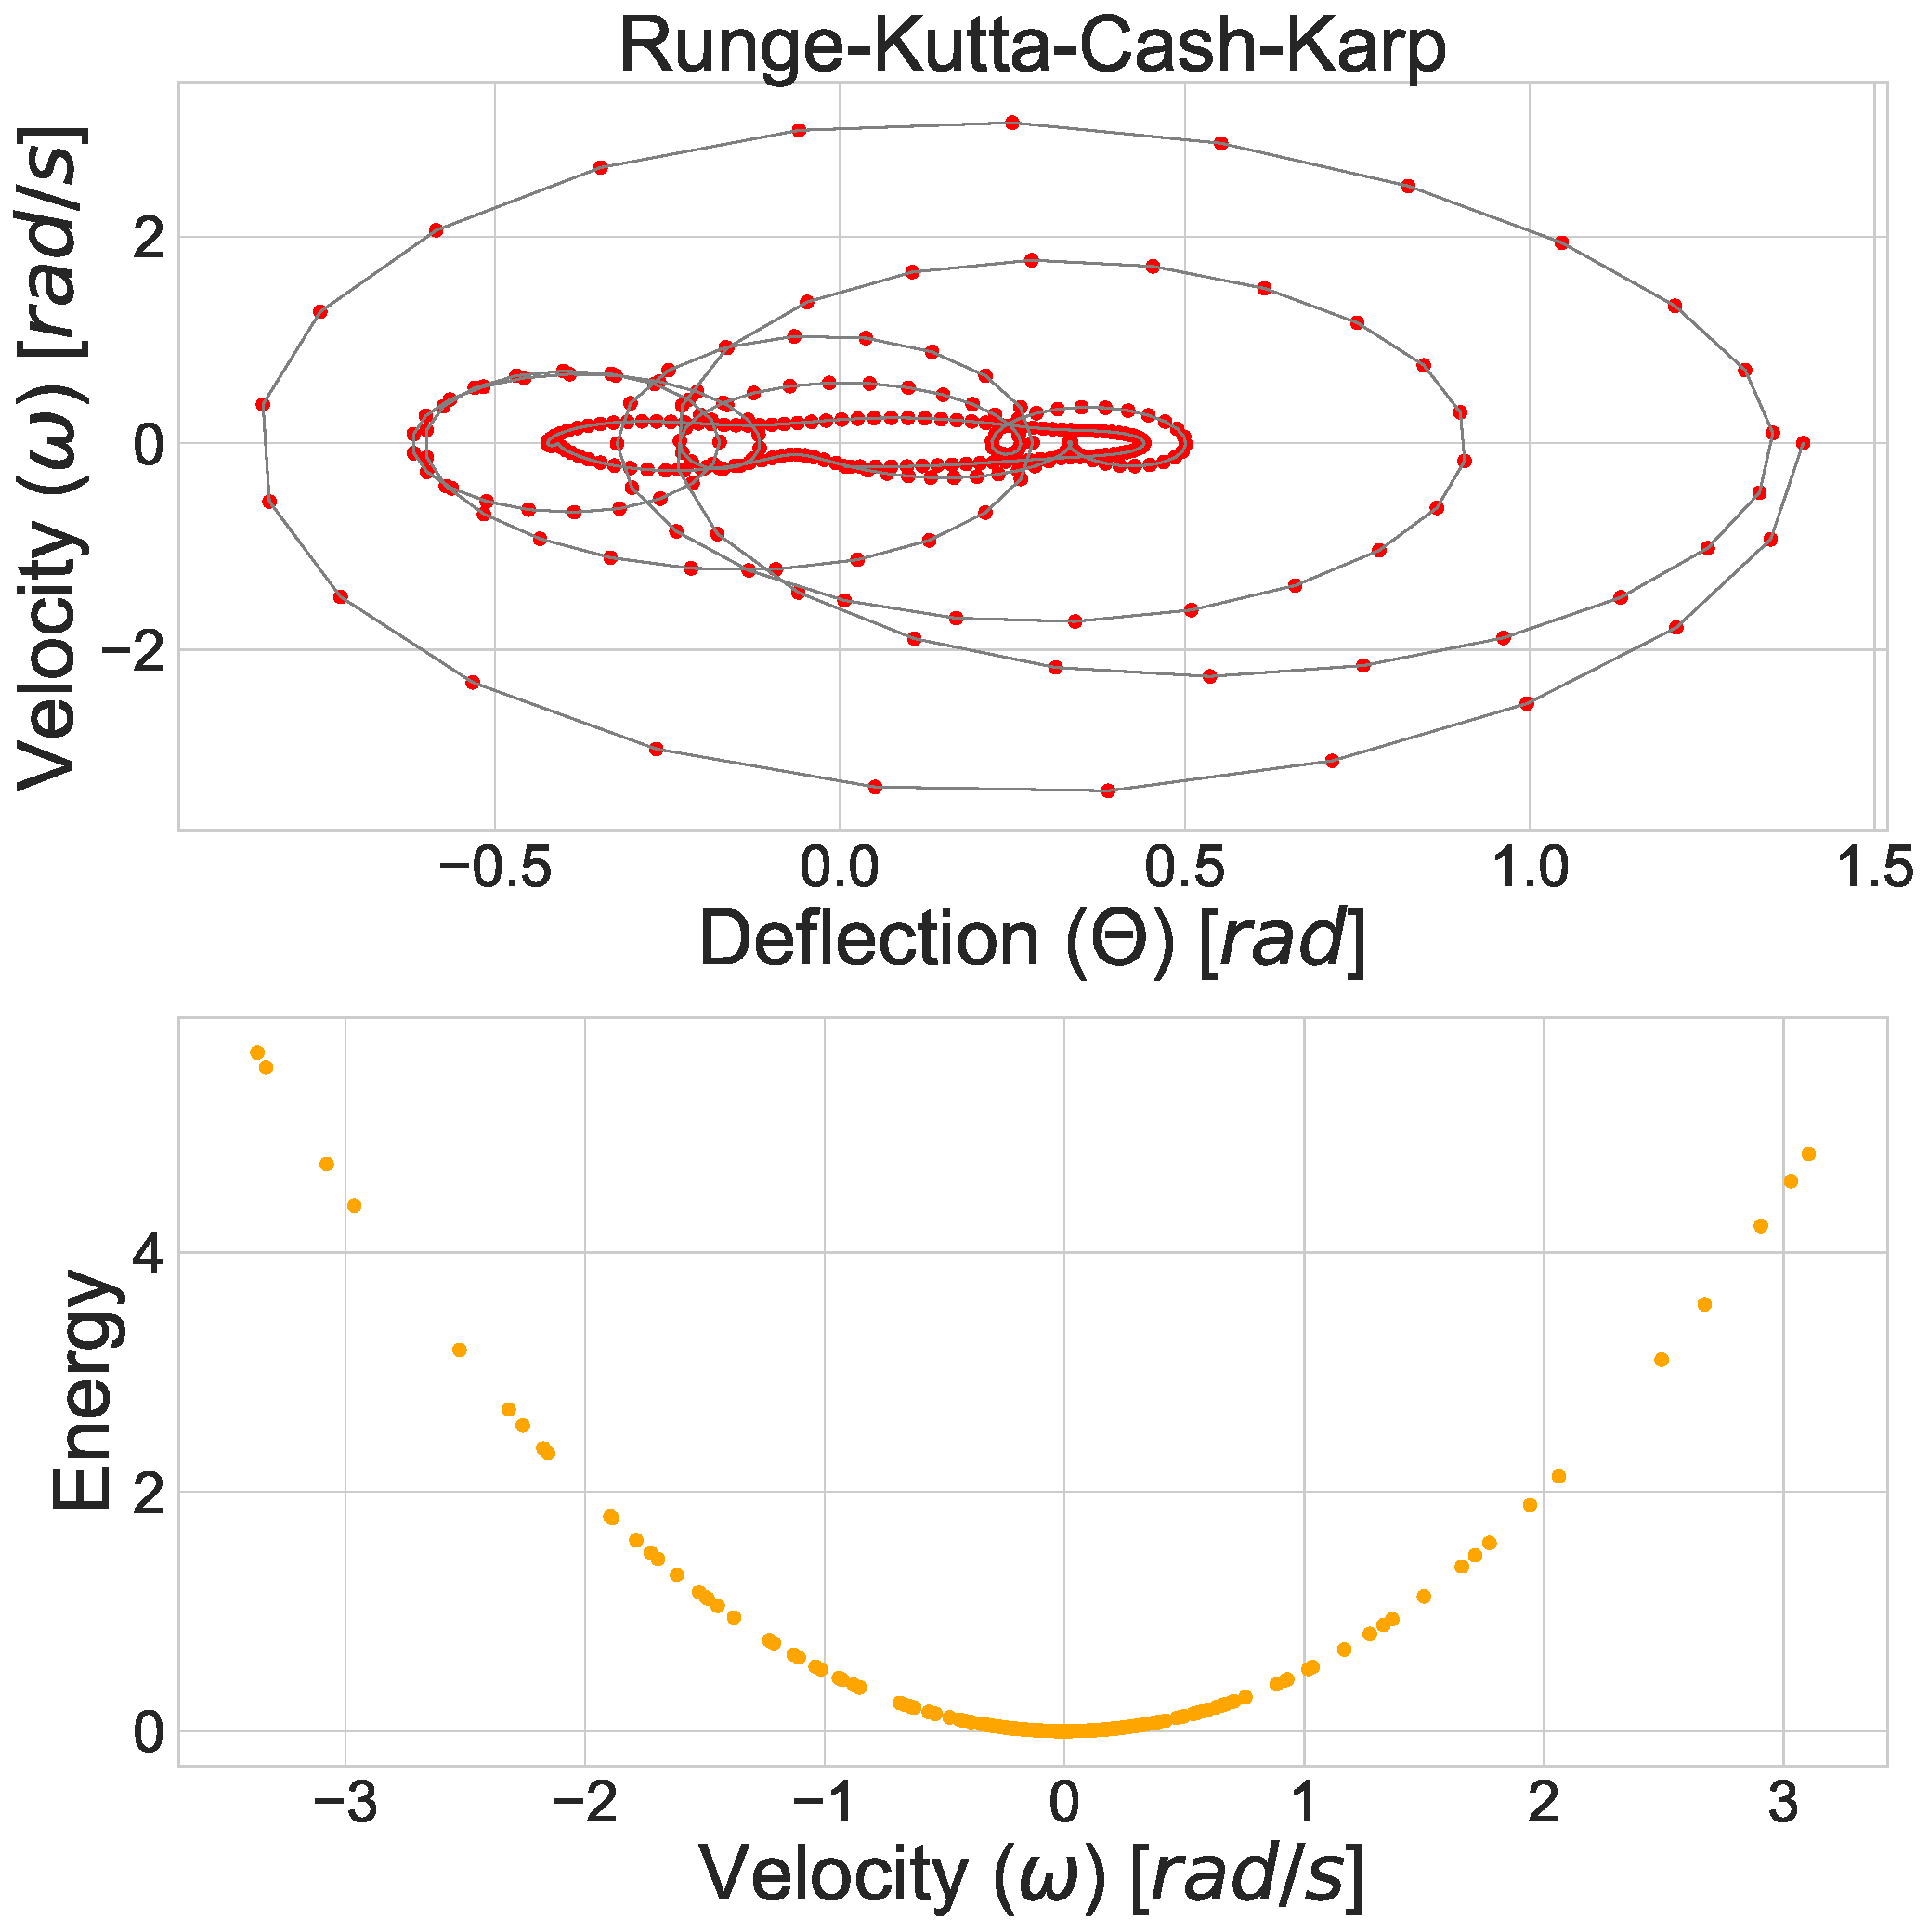
\includegraphics[width=.25\textwidth]{images/phase_energy_rkck_dampeddriven.pdf}}
\captionof{figure}{R-K-C-K\\Damp.-Driv.}\label{fig:34}
\hfill
{\centering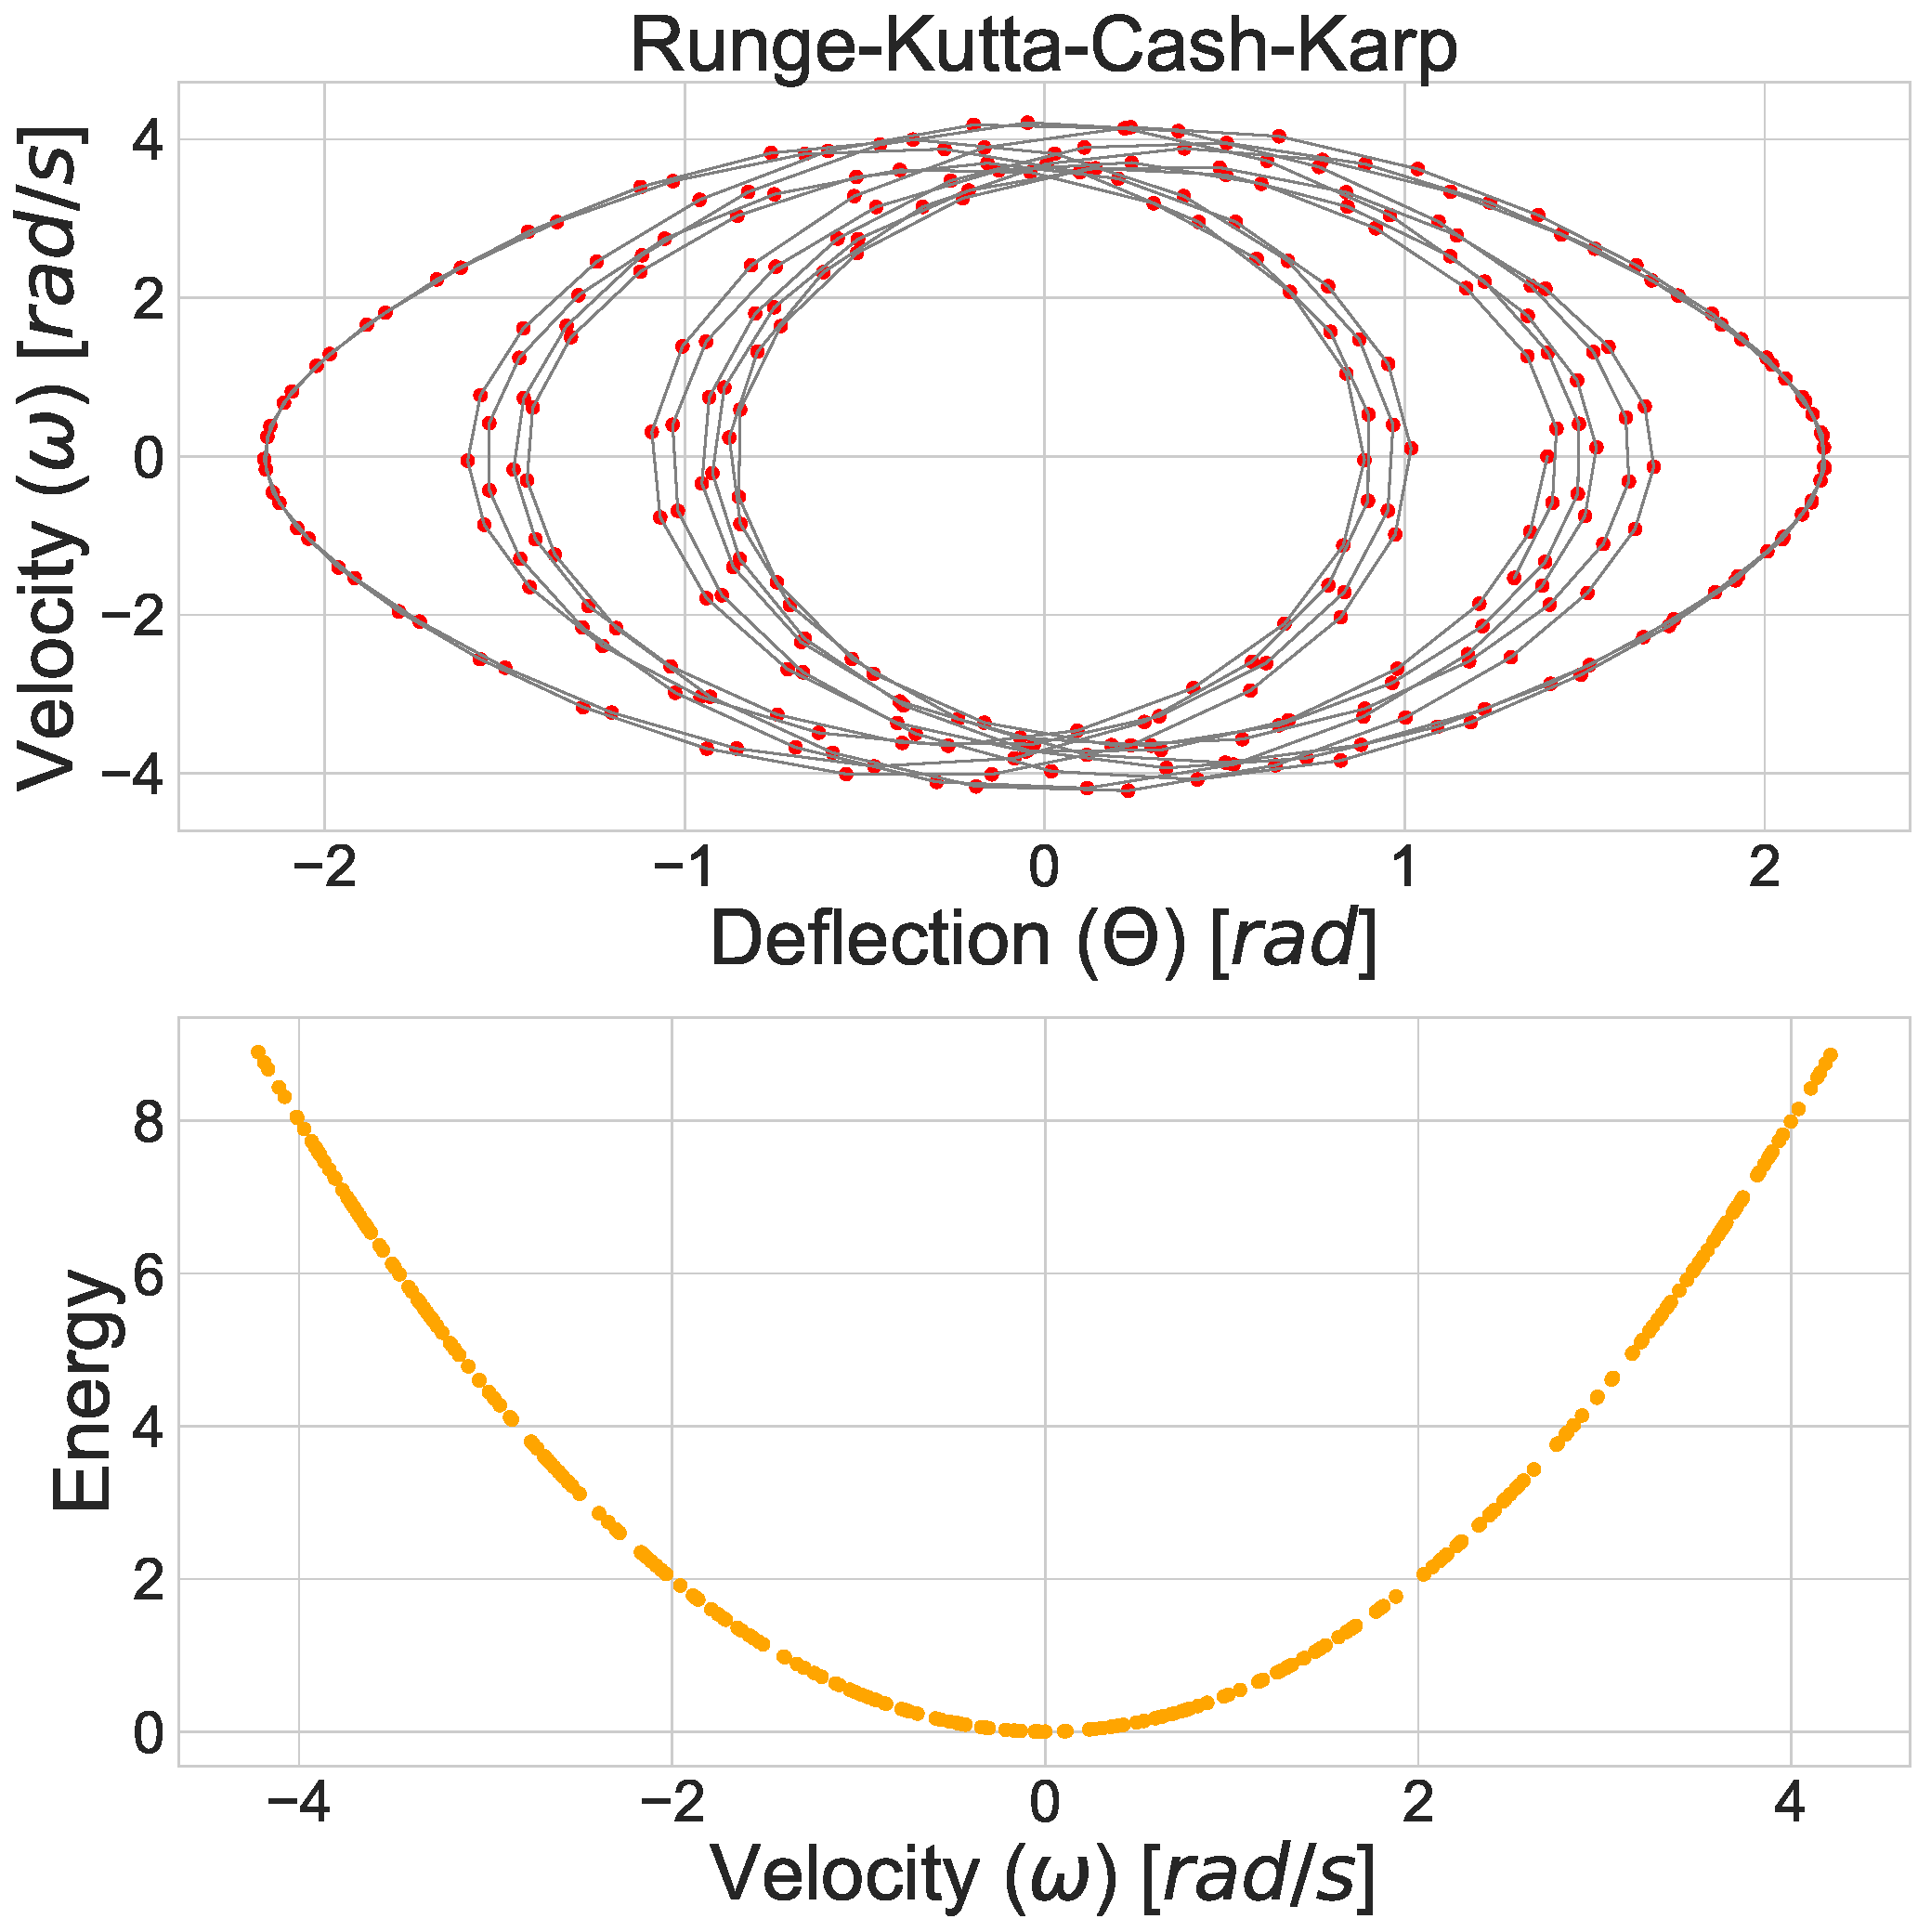
\includegraphics[width=.25\textwidth]{images/phase_energy_rkck_driven.pdf}}
\captionof{figure}{R-K-C-K\\Driv.}\label{fig:35}
\hfill

\end{multicols}
\begin{multicols}{4}

{\centering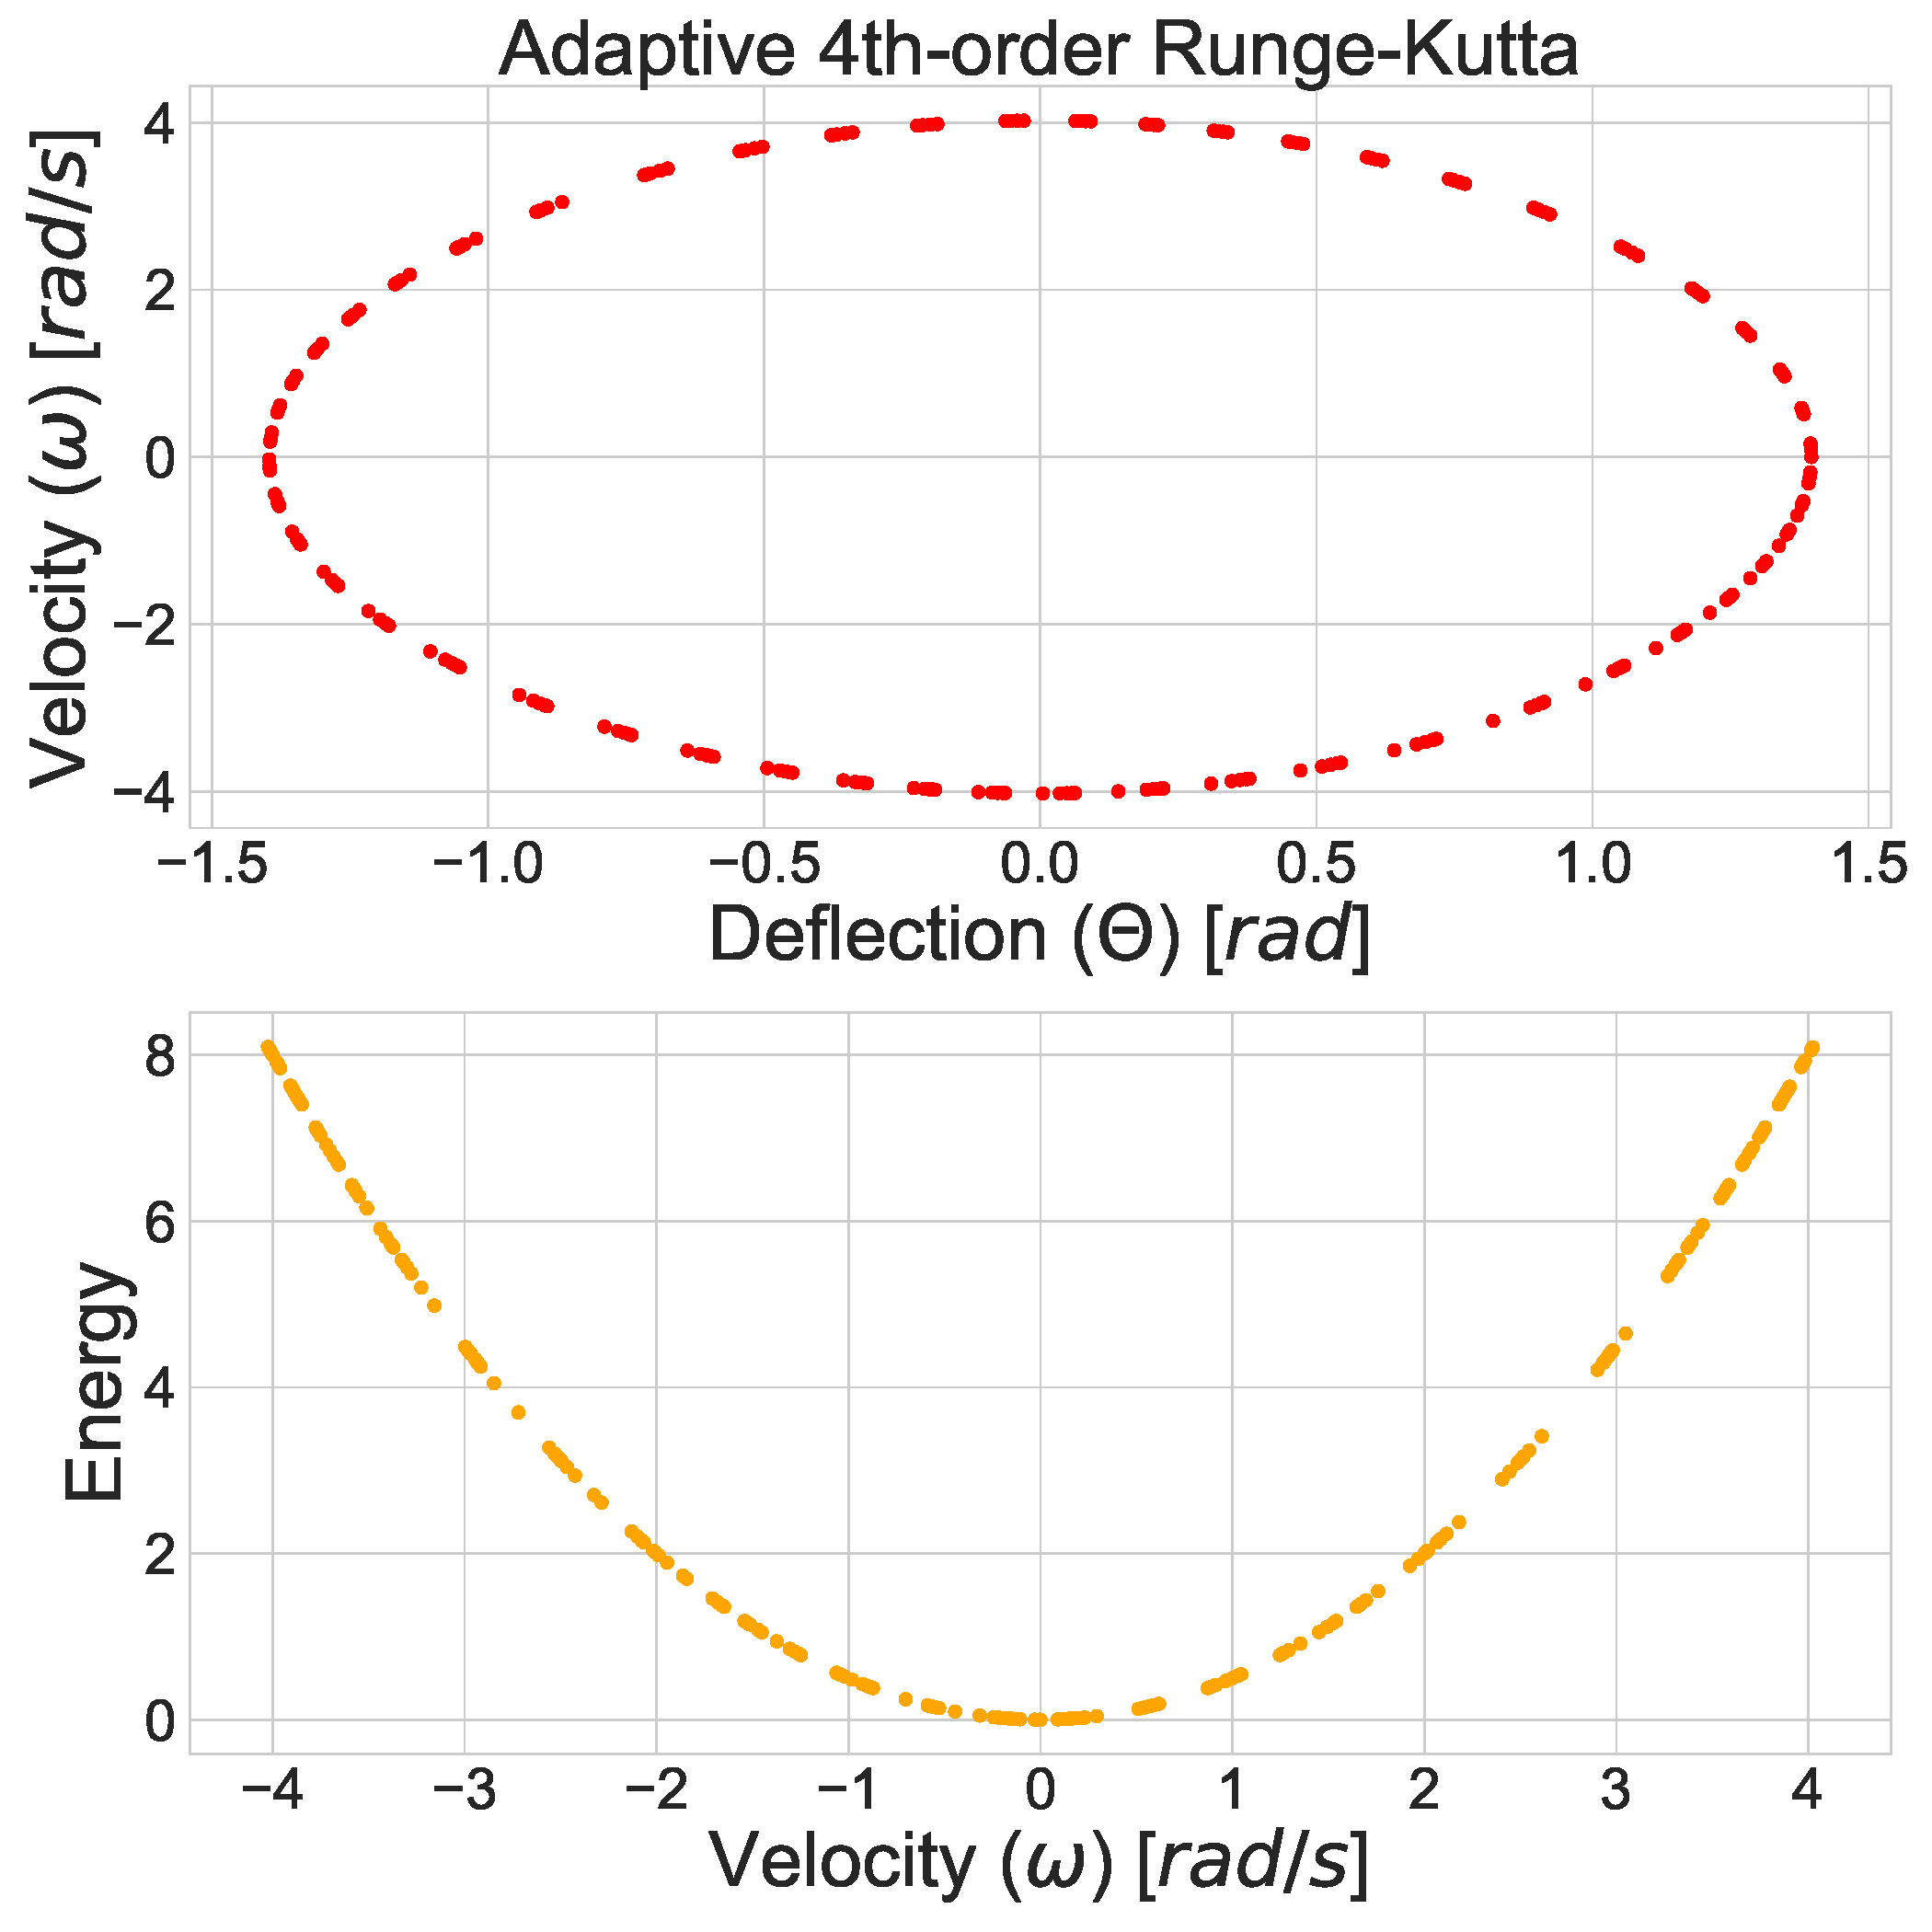
\includegraphics[width=.25\textwidth]{images/phase_energy_adapt_runge.pdf}}
\captionof{figure}{Ad. Runge-Kutta\\Mat.}\label{fig:36}
\hfill
{\centering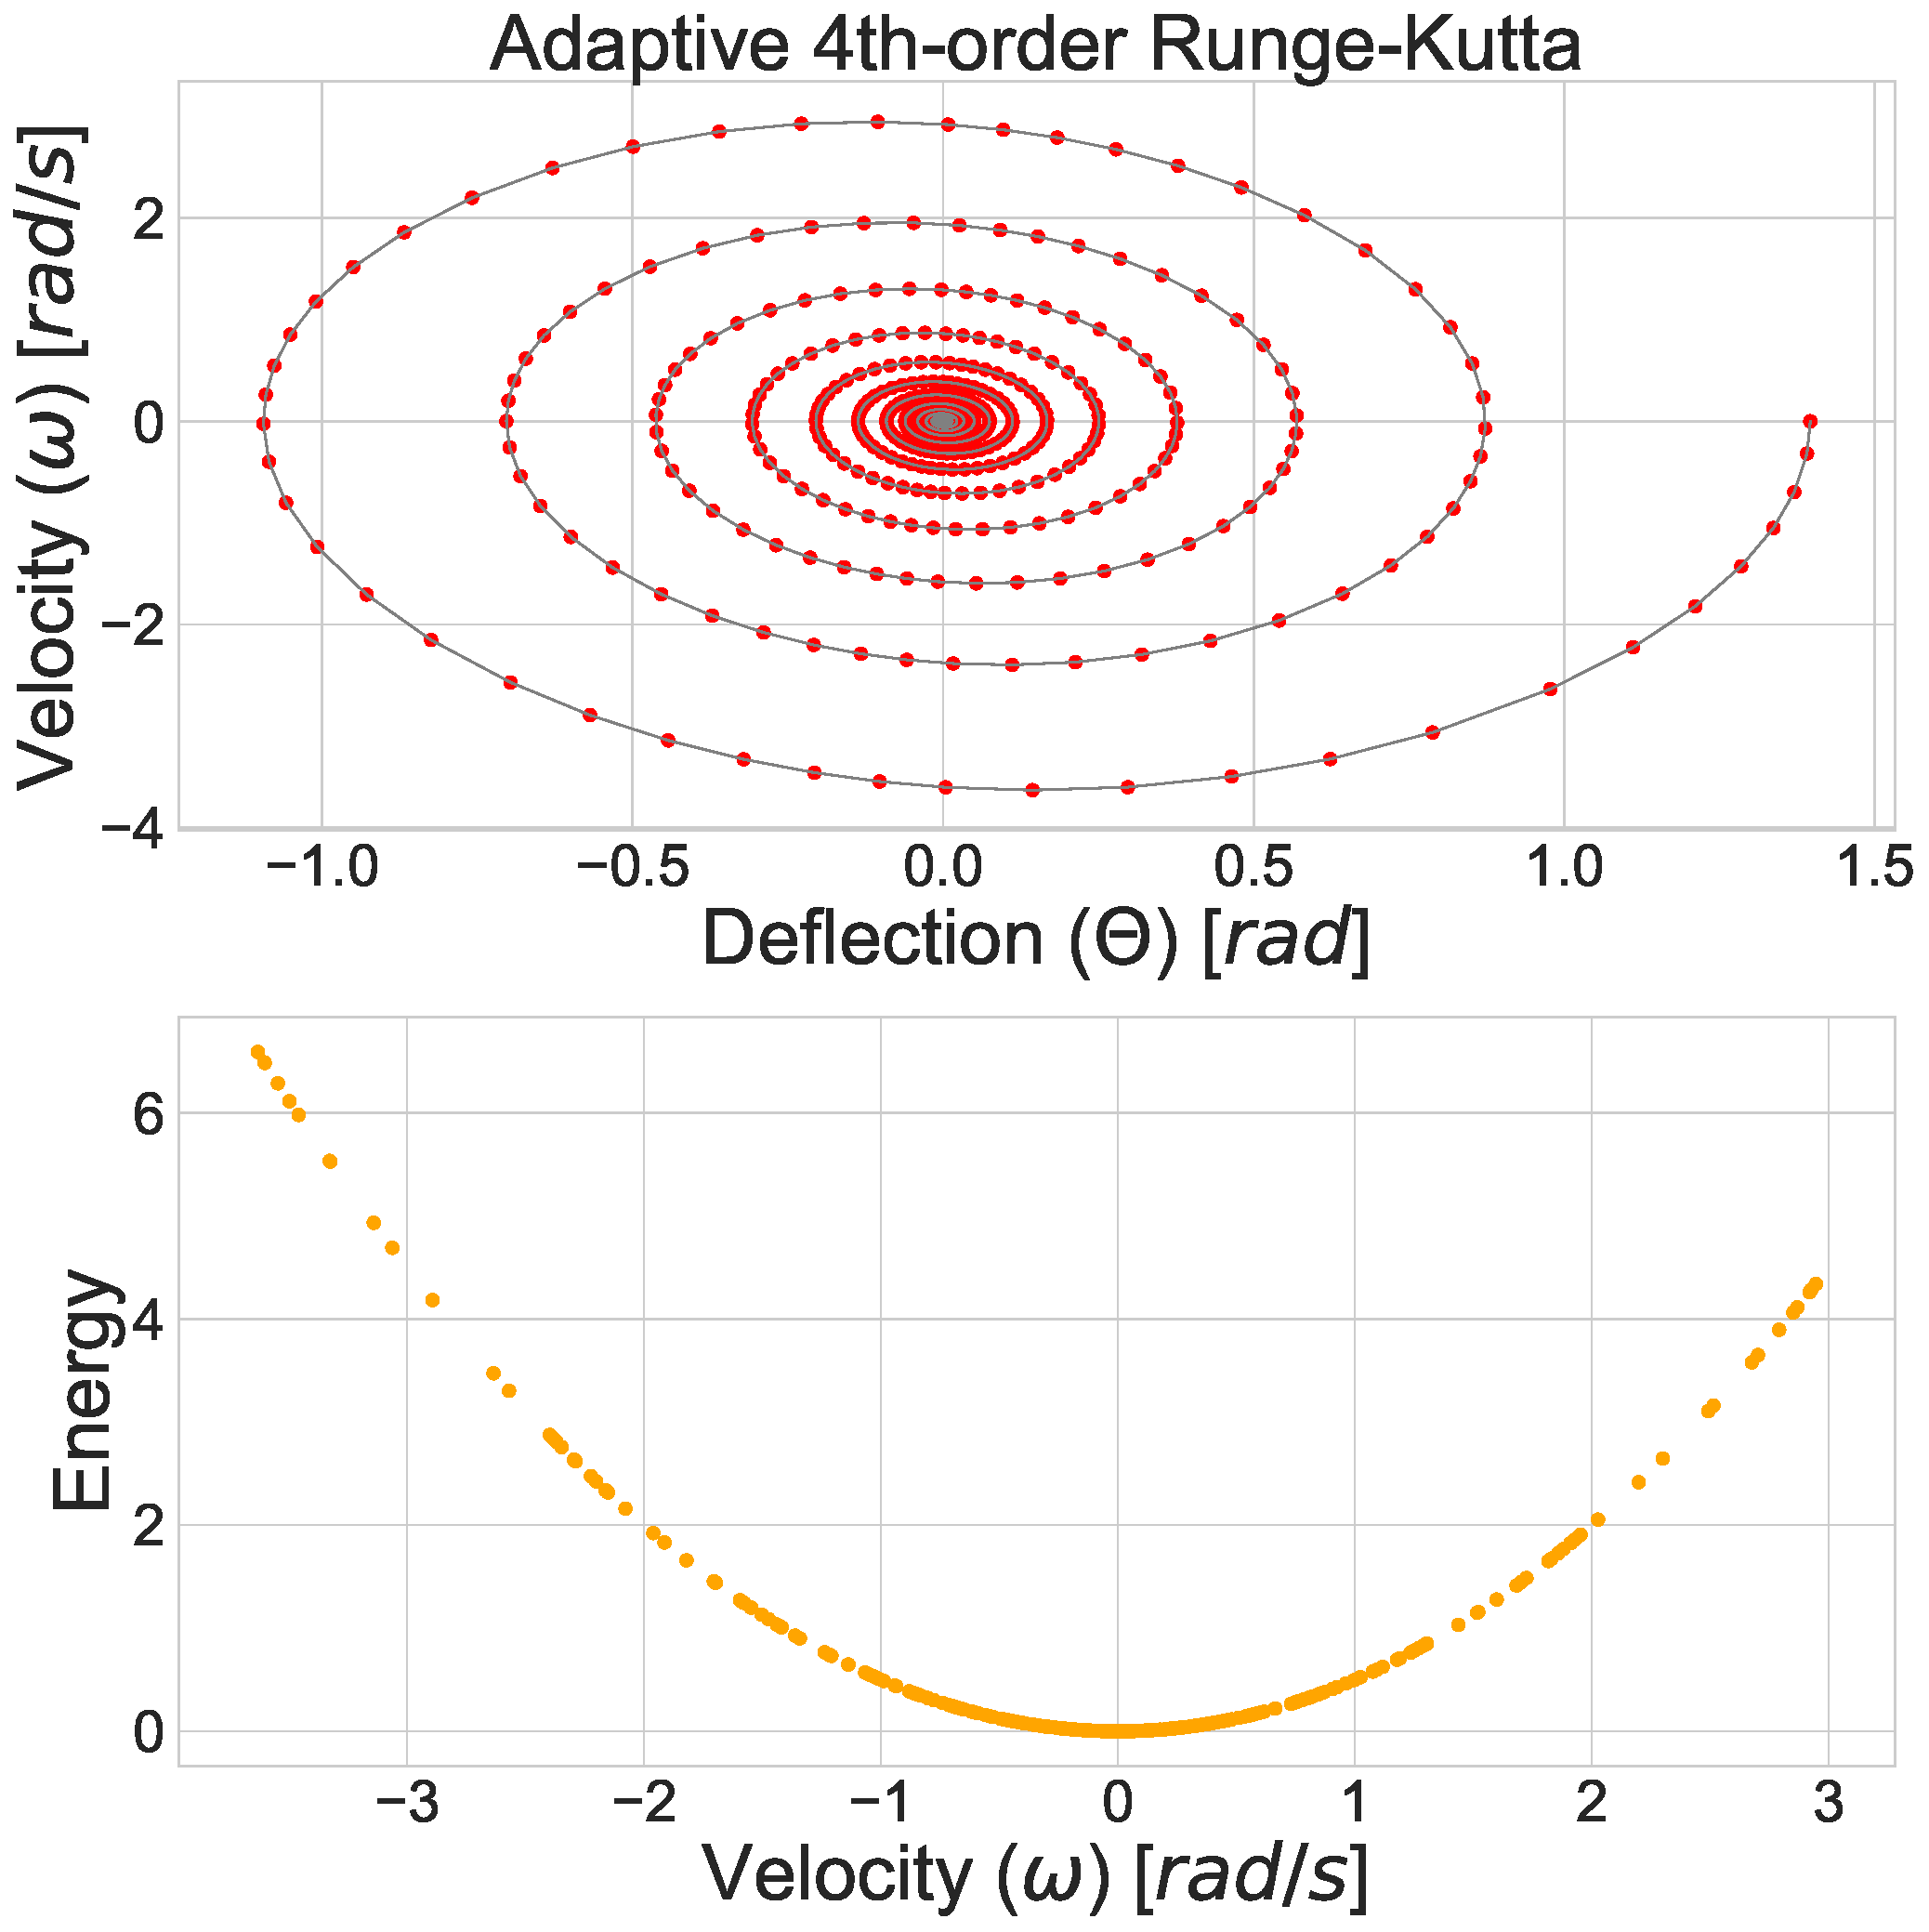
\includegraphics[width=.25\textwidth]{images/phase_energy_adapt_runge_damped.pdf}}
\captionof{figure}{Ad. Runge-Kutta\\Damp.}\label{fig:37}
\hfill
{\centering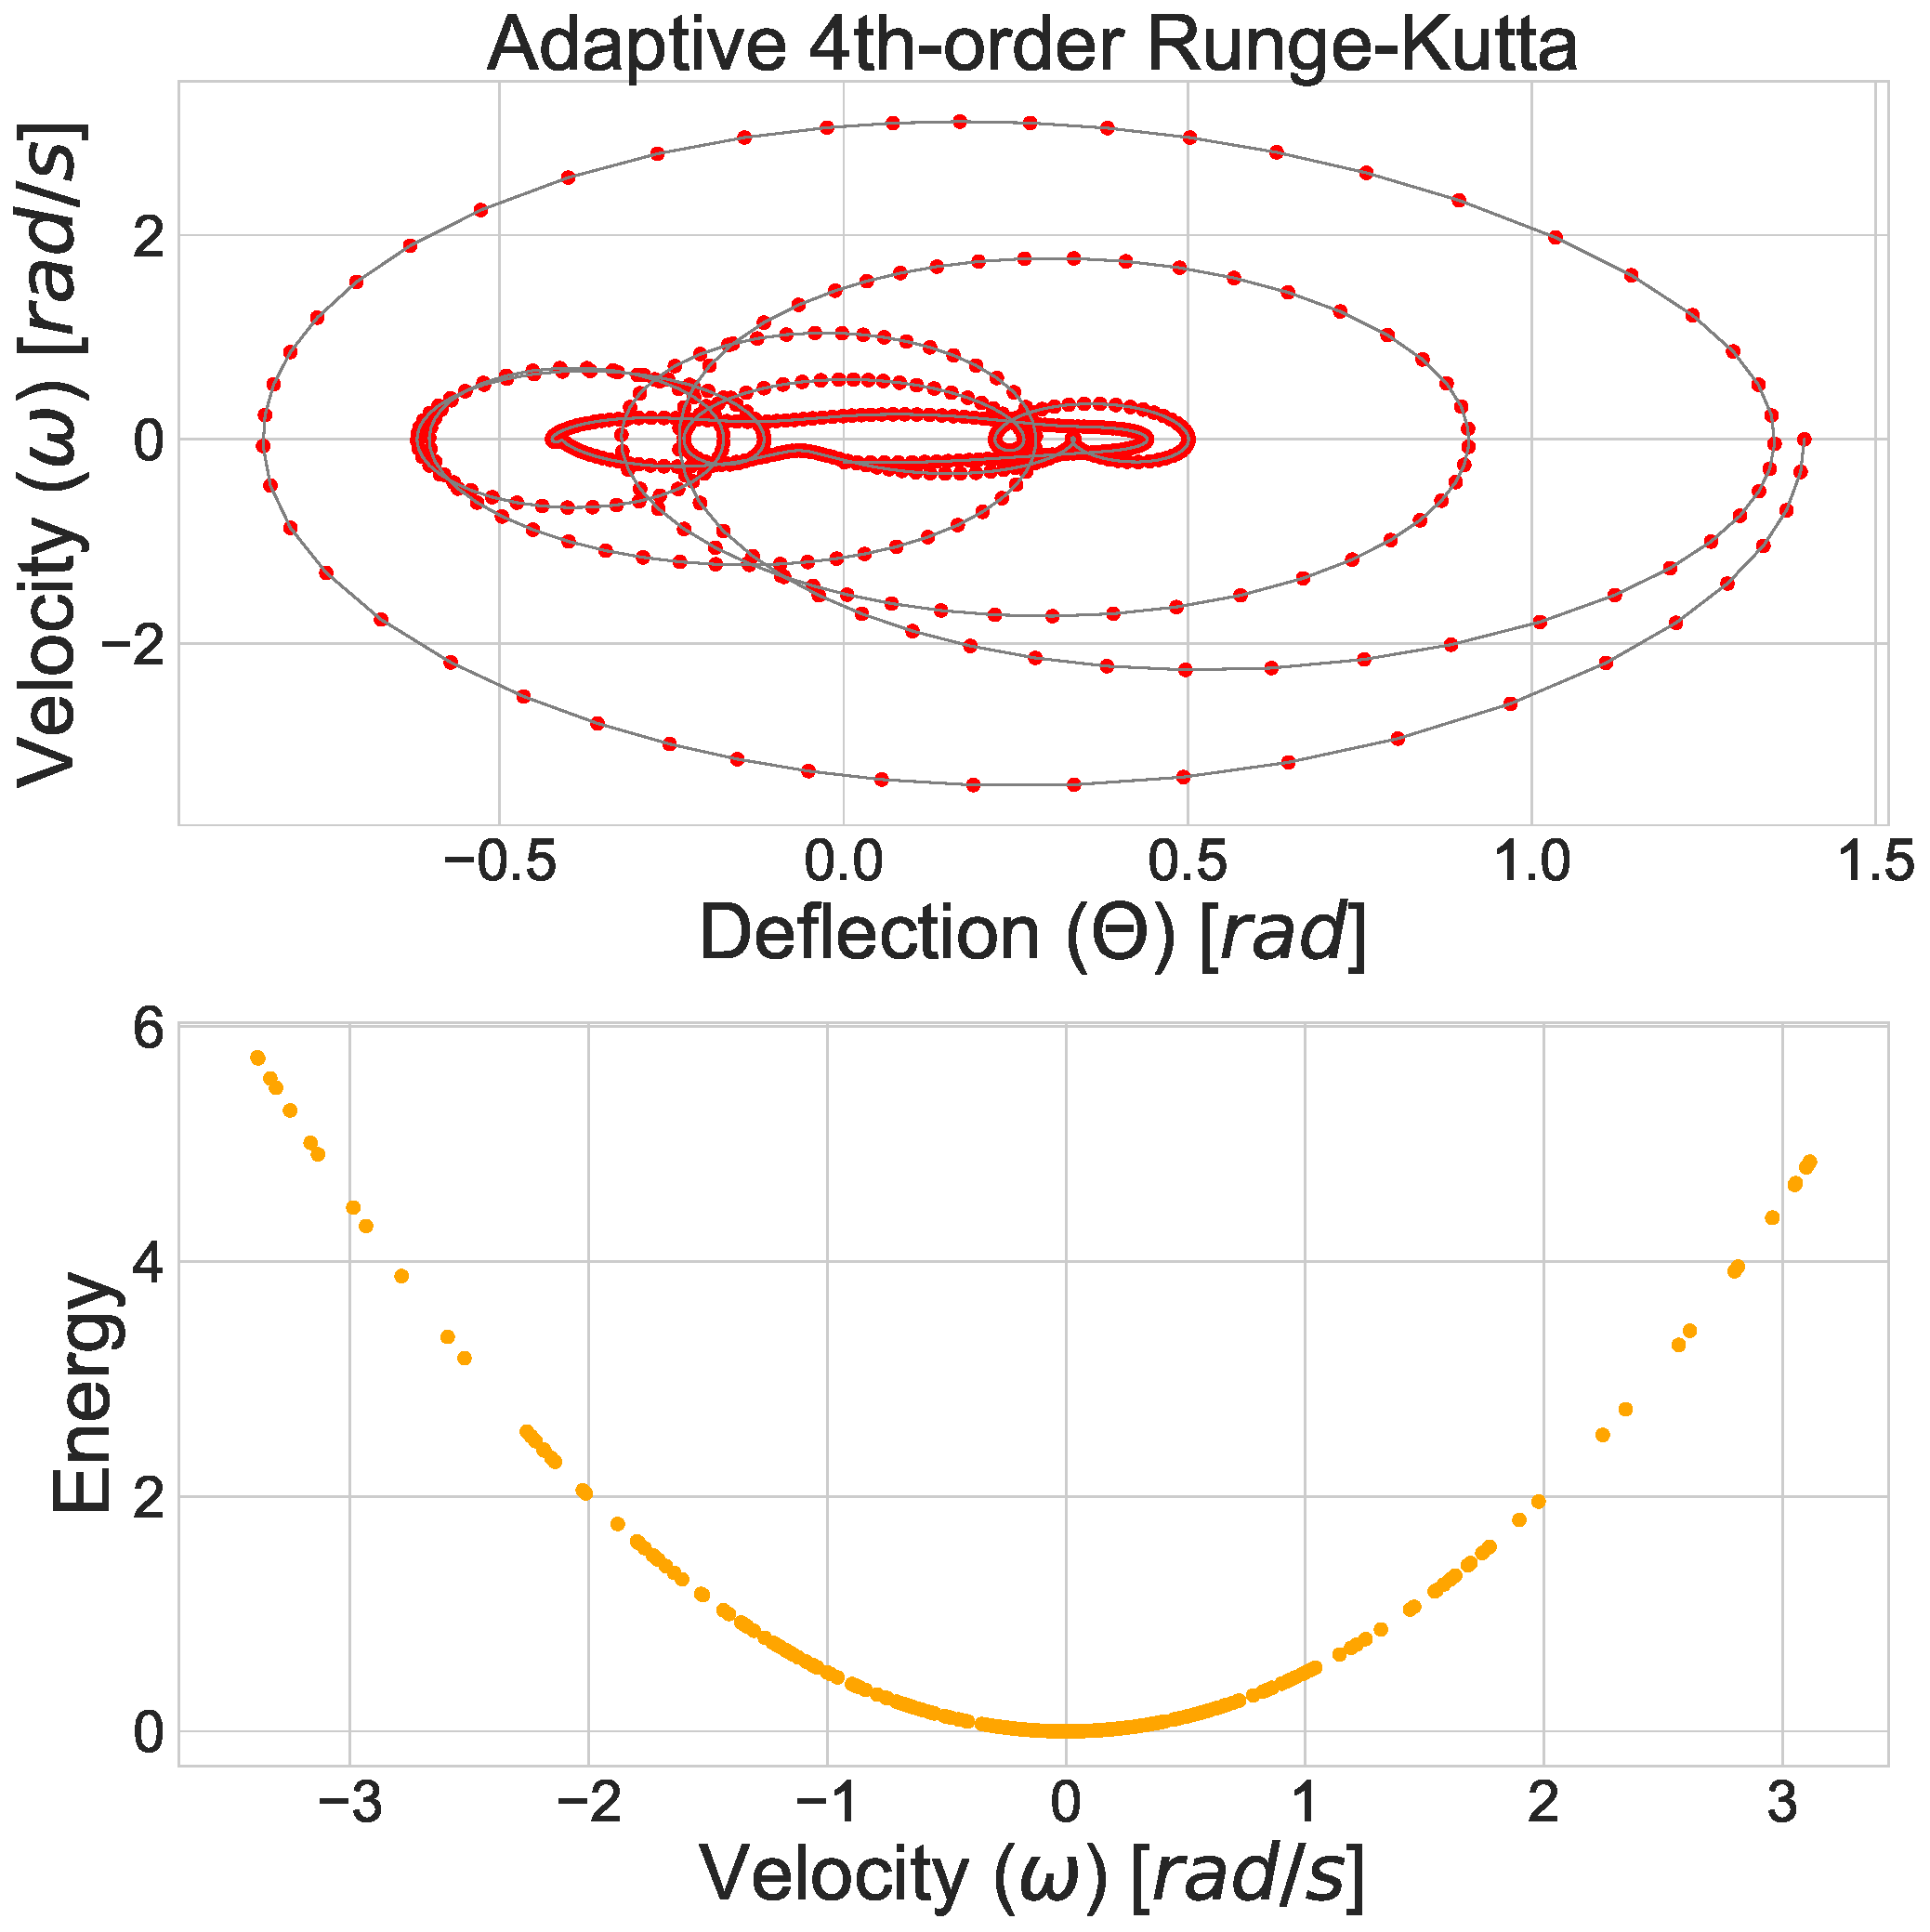
\includegraphics[width=.25\textwidth]{images/phase_energy_adapt_runge_dampeddriven.pdf}}
\captionof{figure}{Ad. Runge-Kutta\\Damp.-Driv.}\label{fig:38}
\hfill
{\centering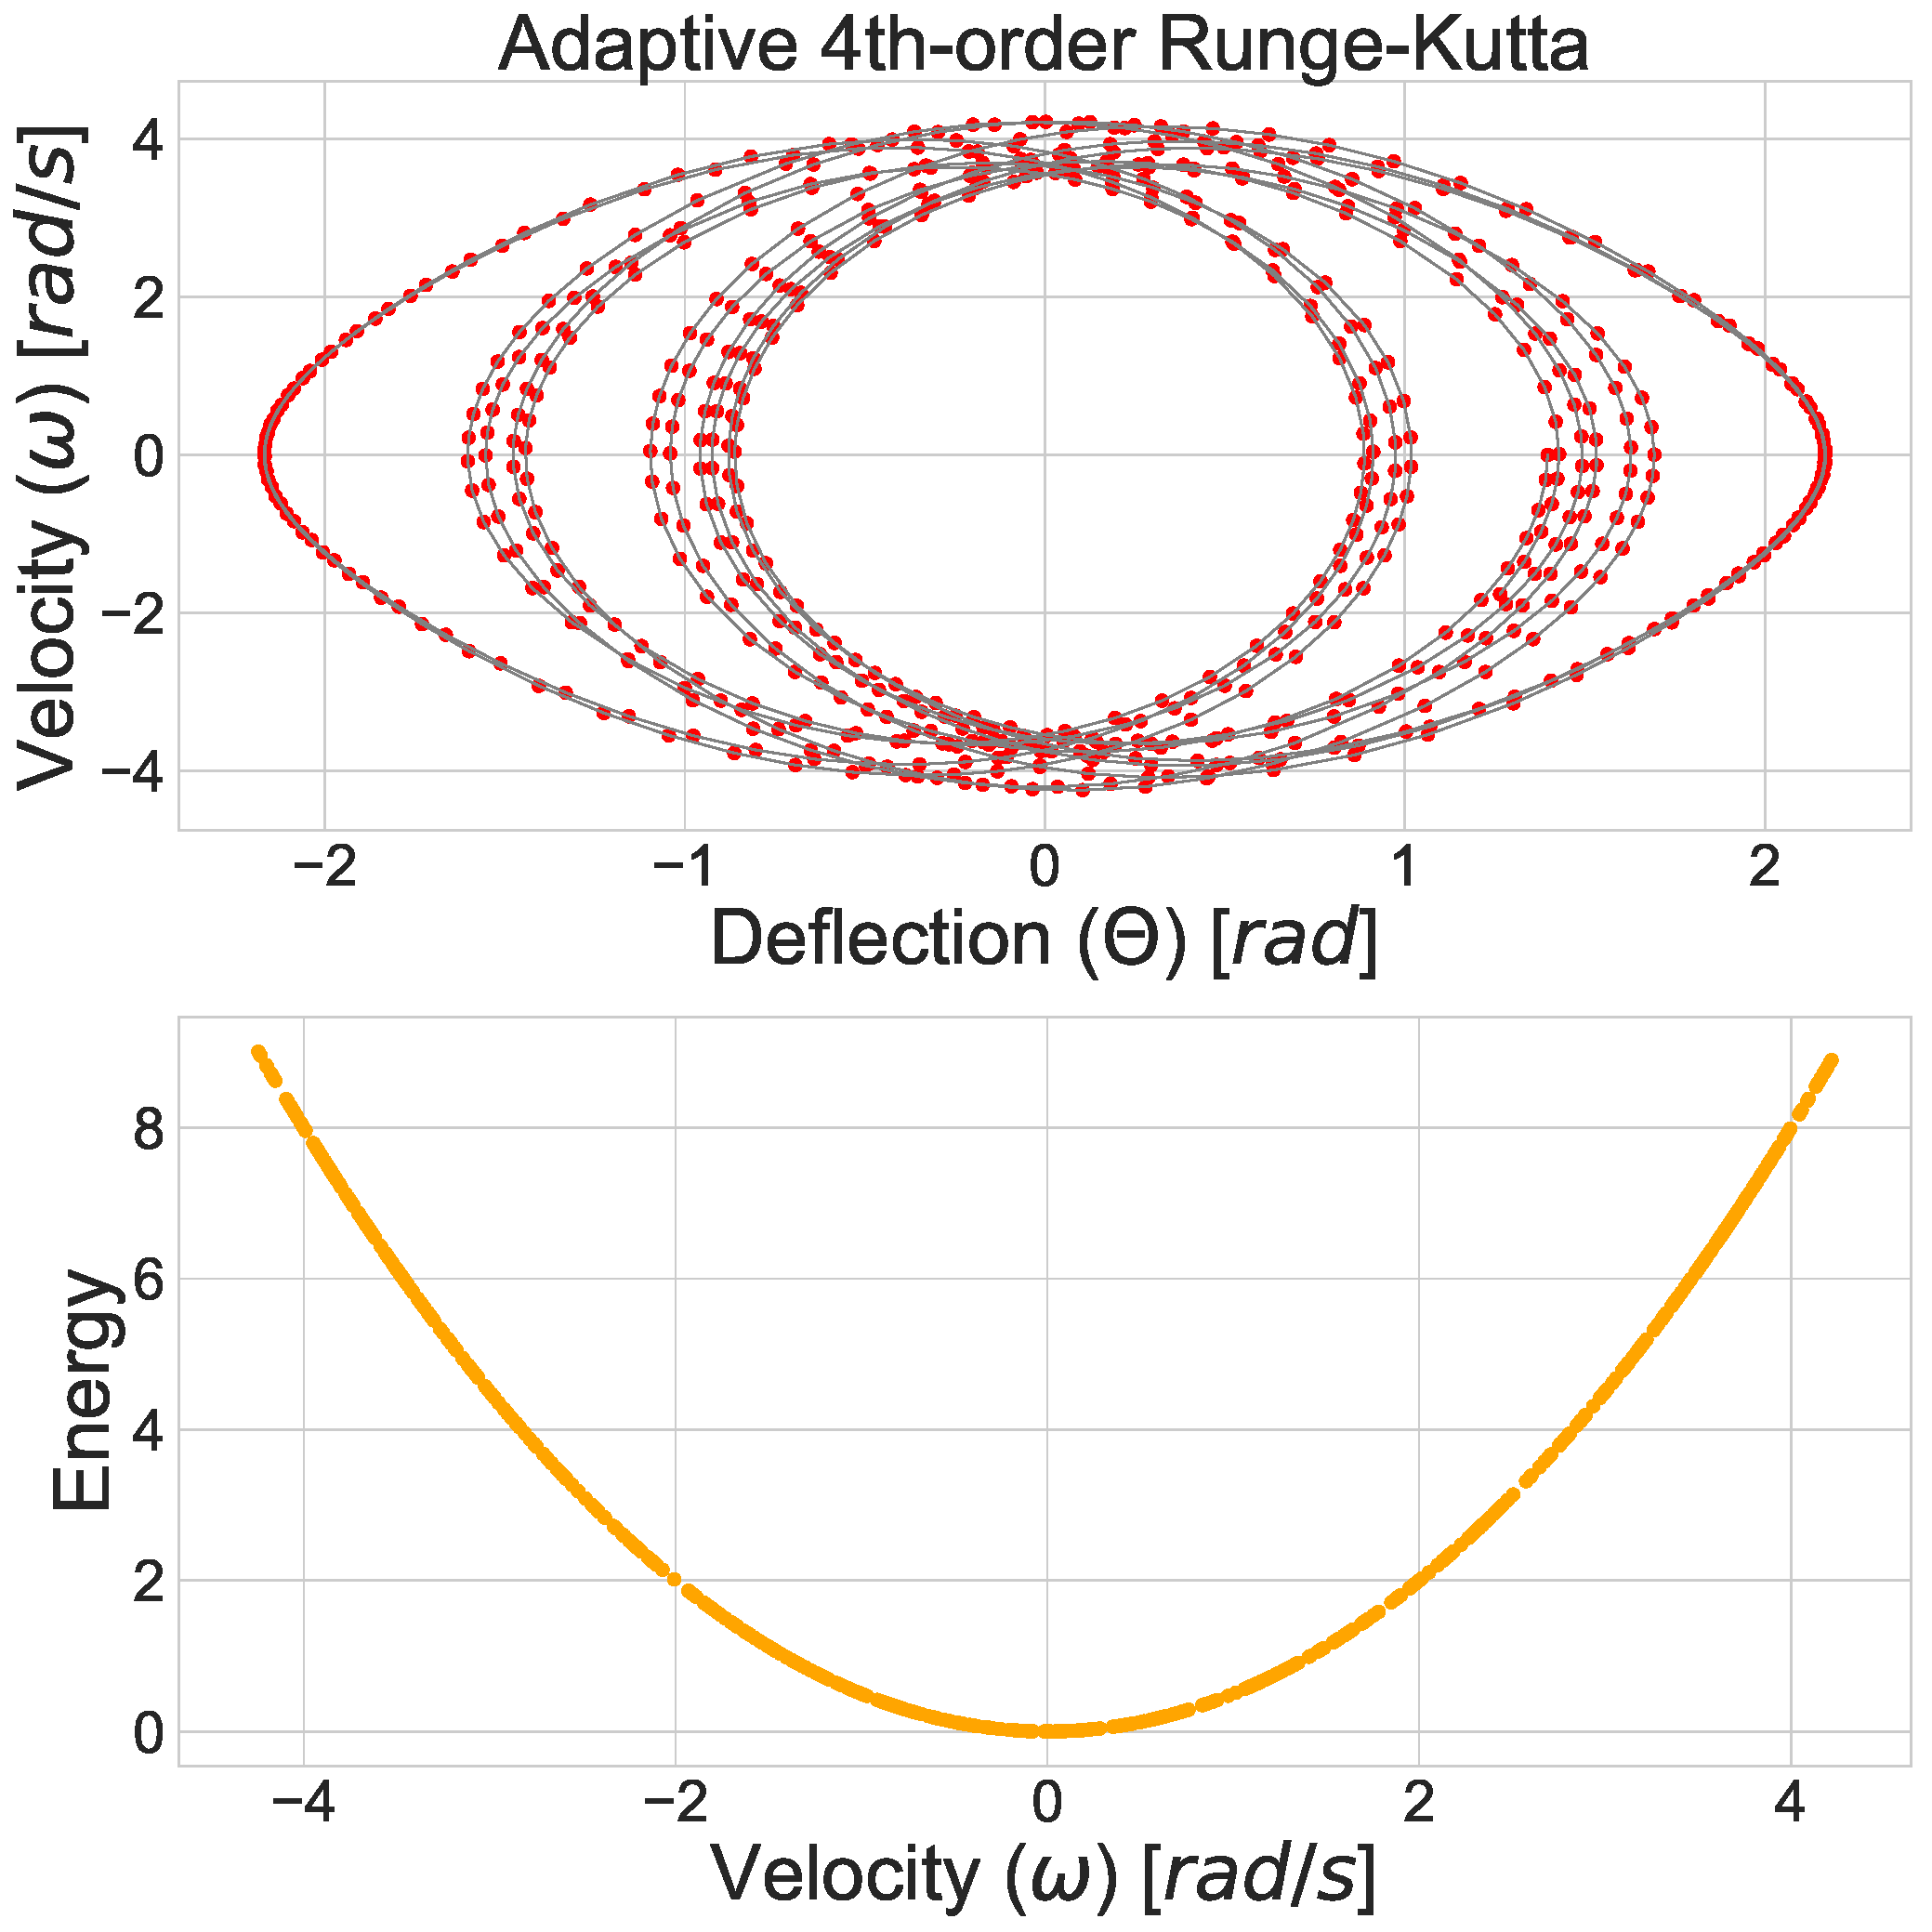
\includegraphics[width=.25\textwidth]{images/phase_energy_adapt_runge_driven.pdf}}
\captionof{figure}{Ad. Runge-Kutta\\Driv.}\label{fig:39}
\hfill

\end{multicols}
\begin{multicols}{4}

{\centering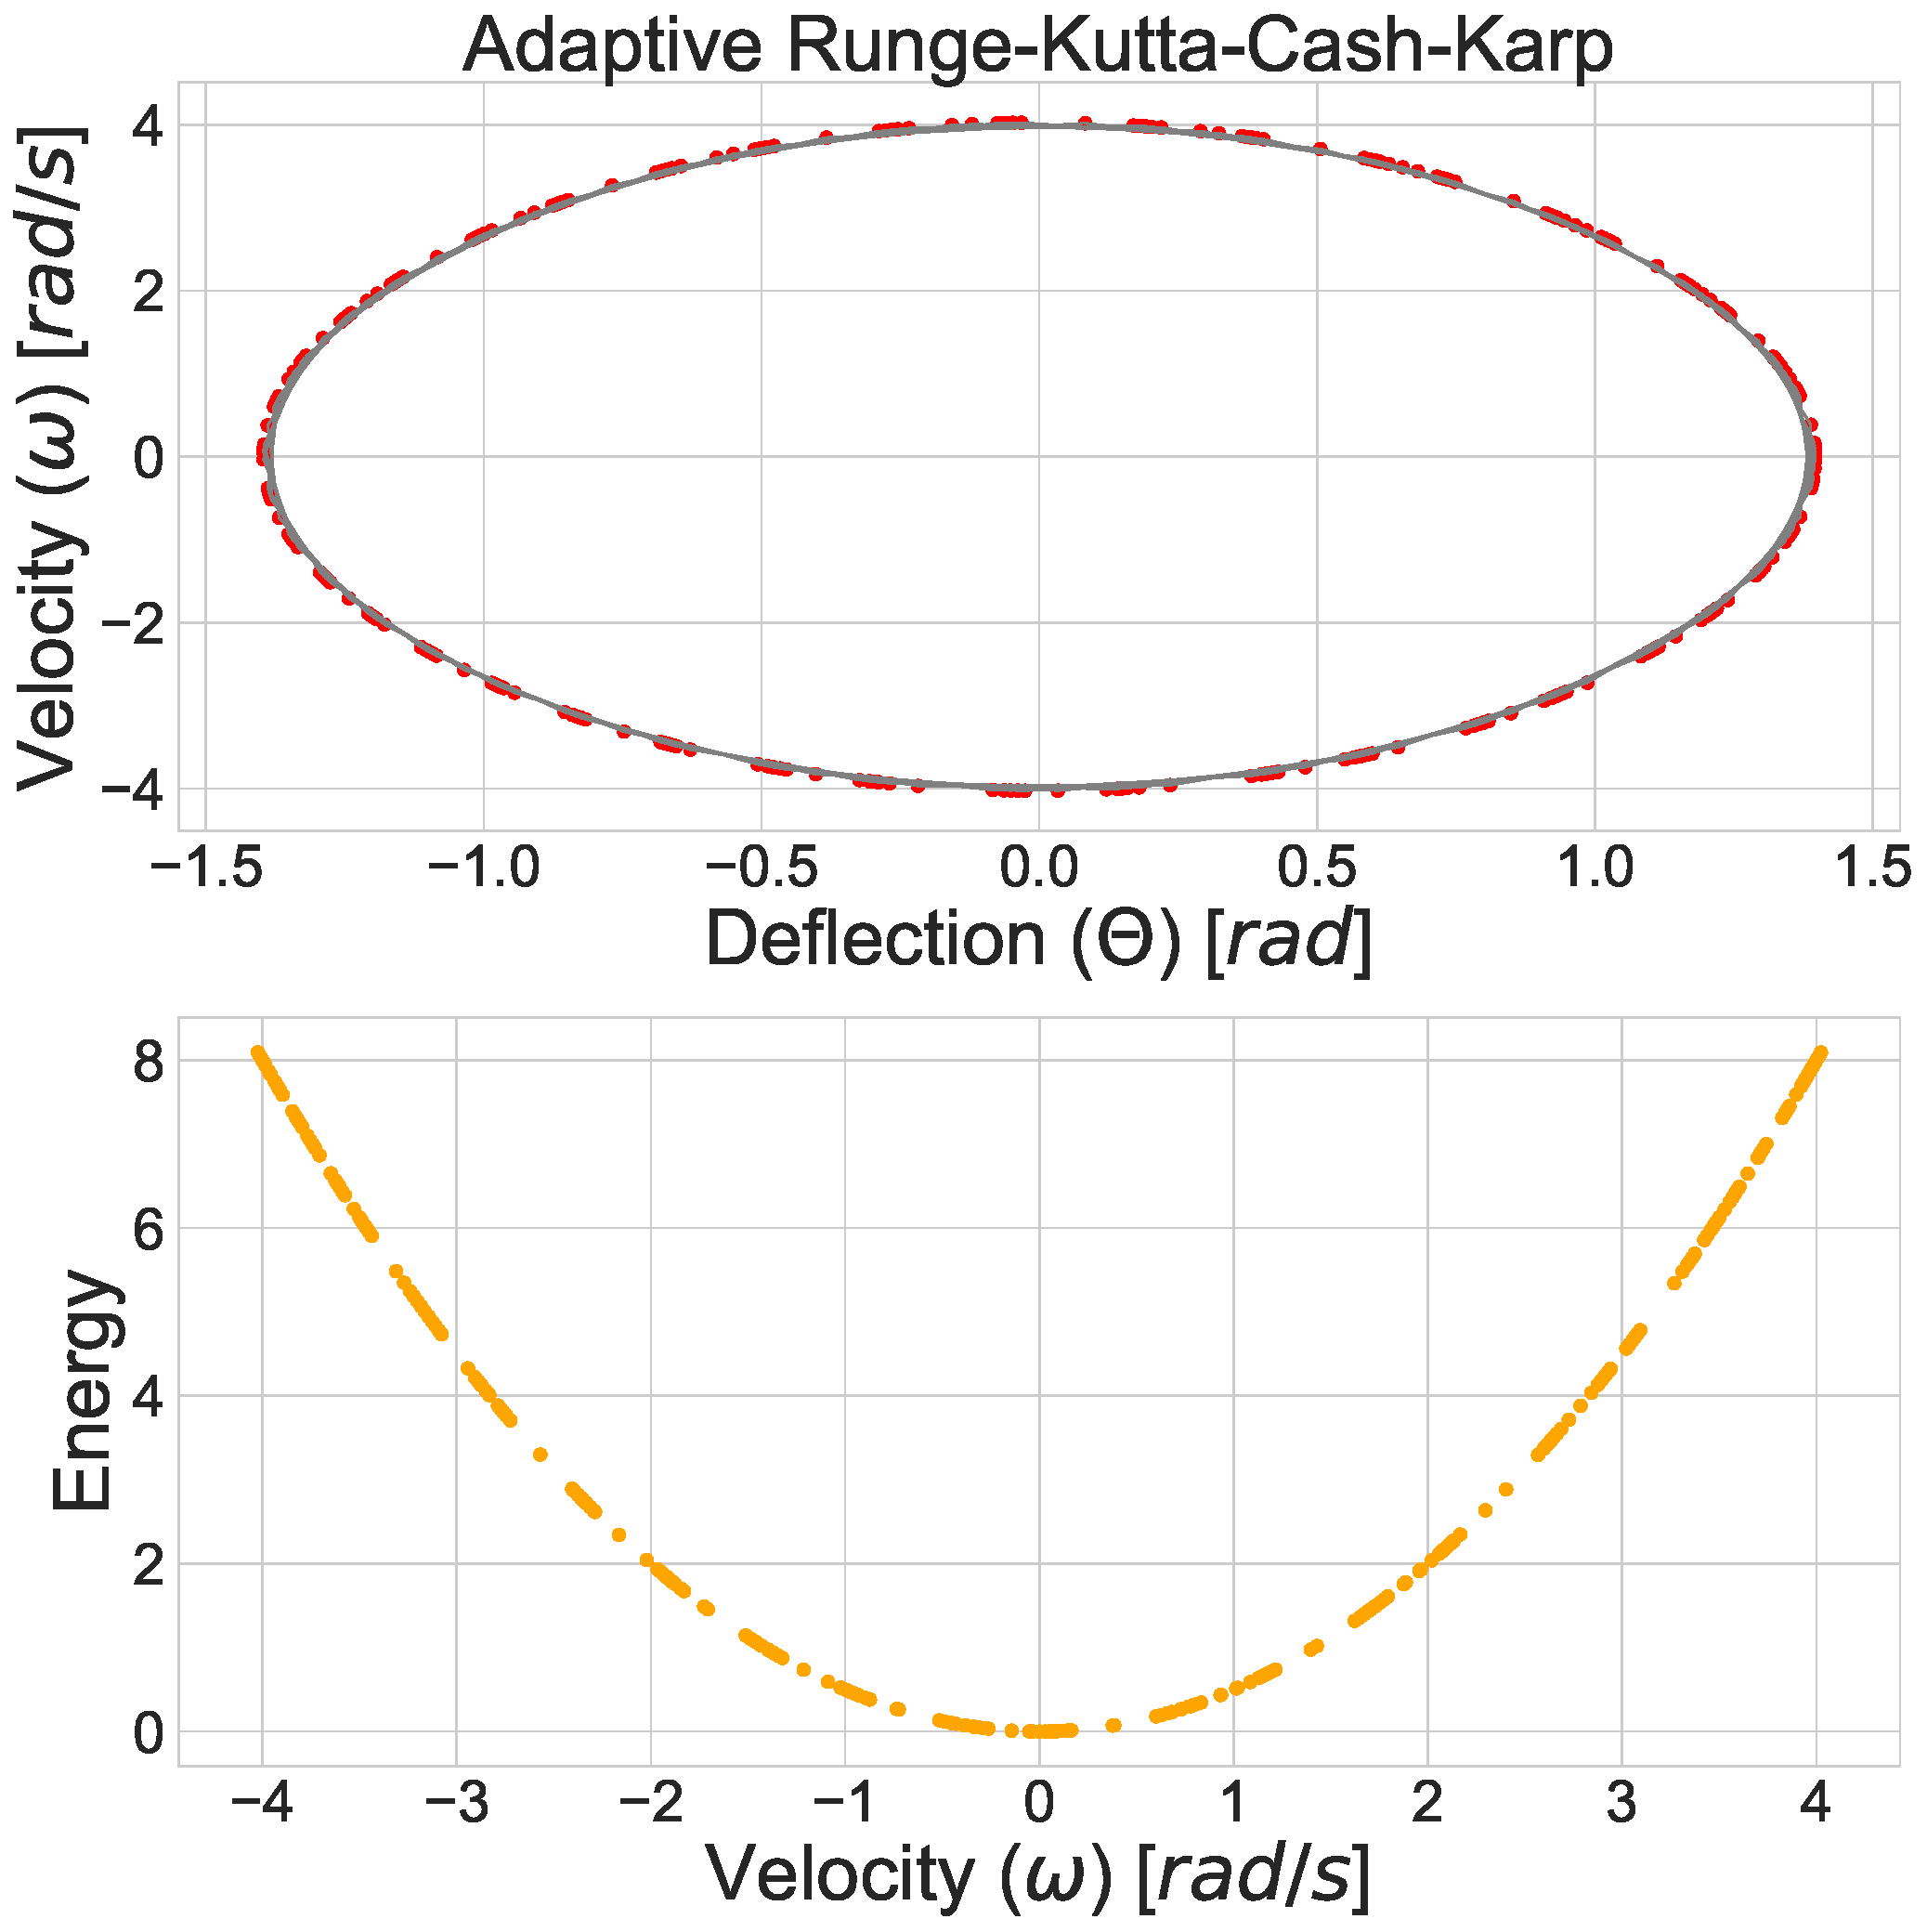
\includegraphics[width=.25\textwidth]{images/phase_energy_adapt_rkck.pdf}}
\captionof{figure}{Ad. R-K-C-K\\Mat.}\label{fig:40}
\hfill
{\centering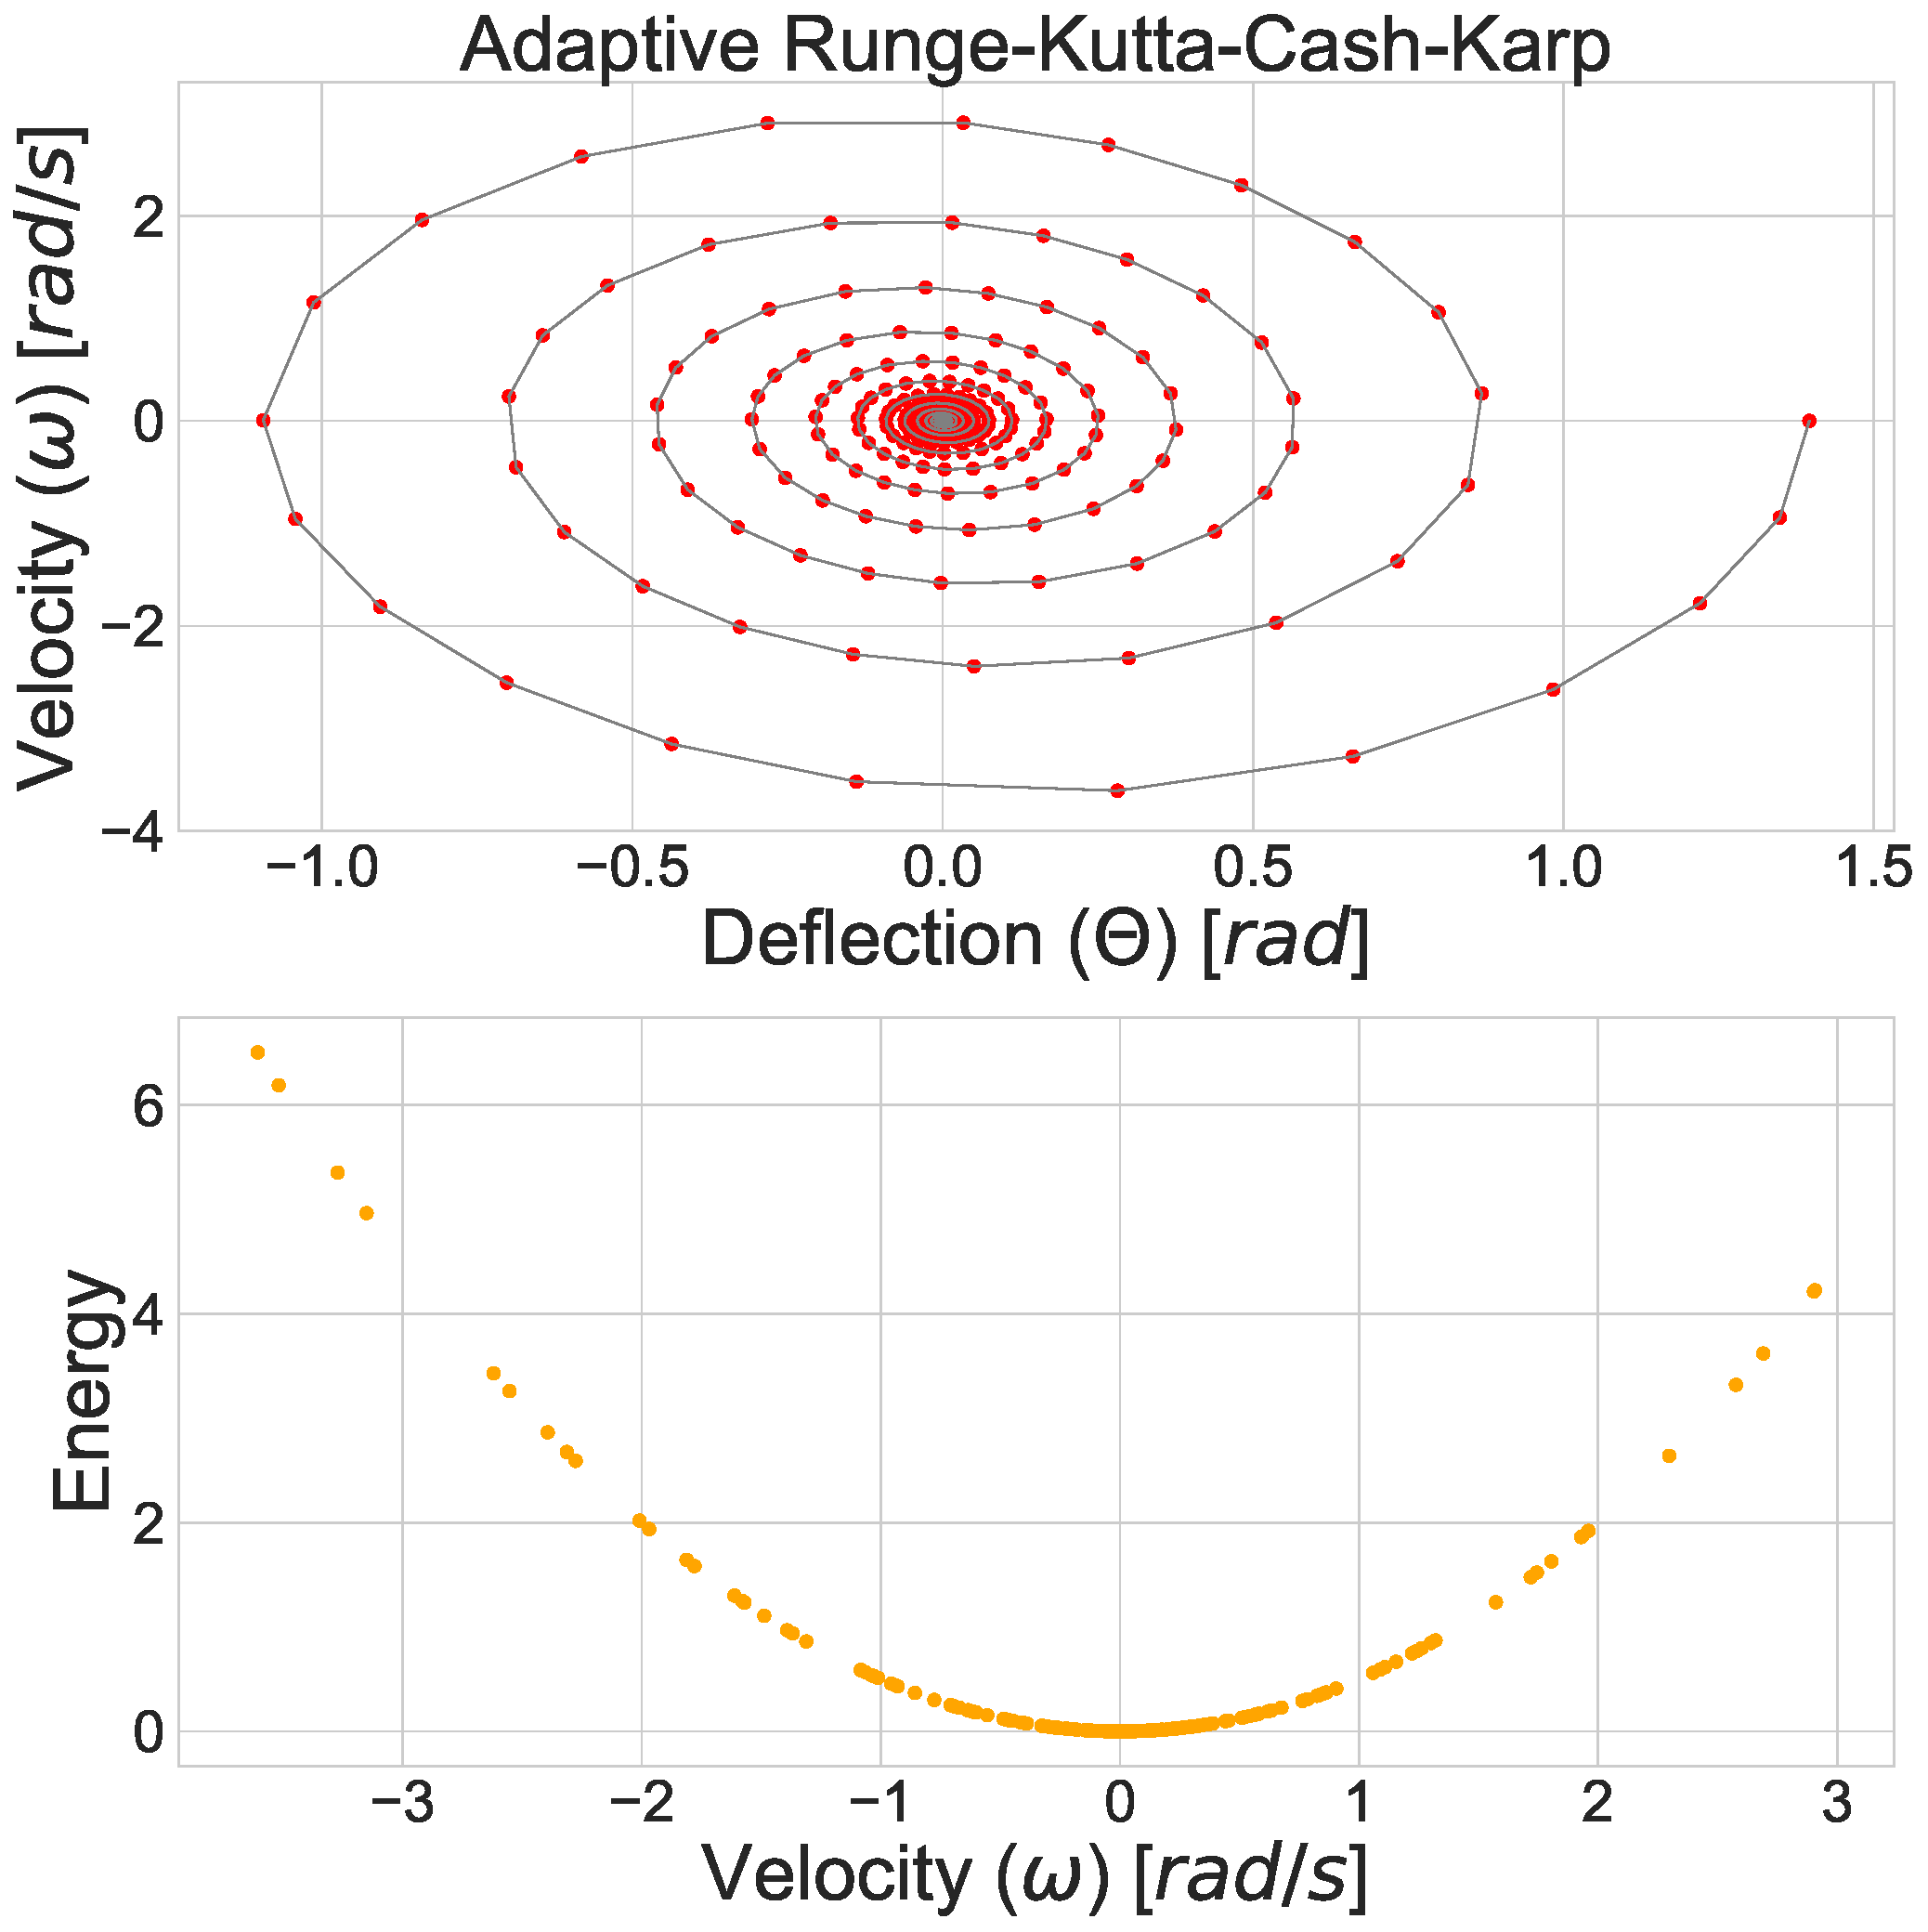
\includegraphics[width=.25\textwidth]{images/phase_energy_adapt_rkck_damped.pdf}}
\captionof{figure}{Ad. R-K-C-K\\Damp.}\label{fig:41}
\hfill
{\centering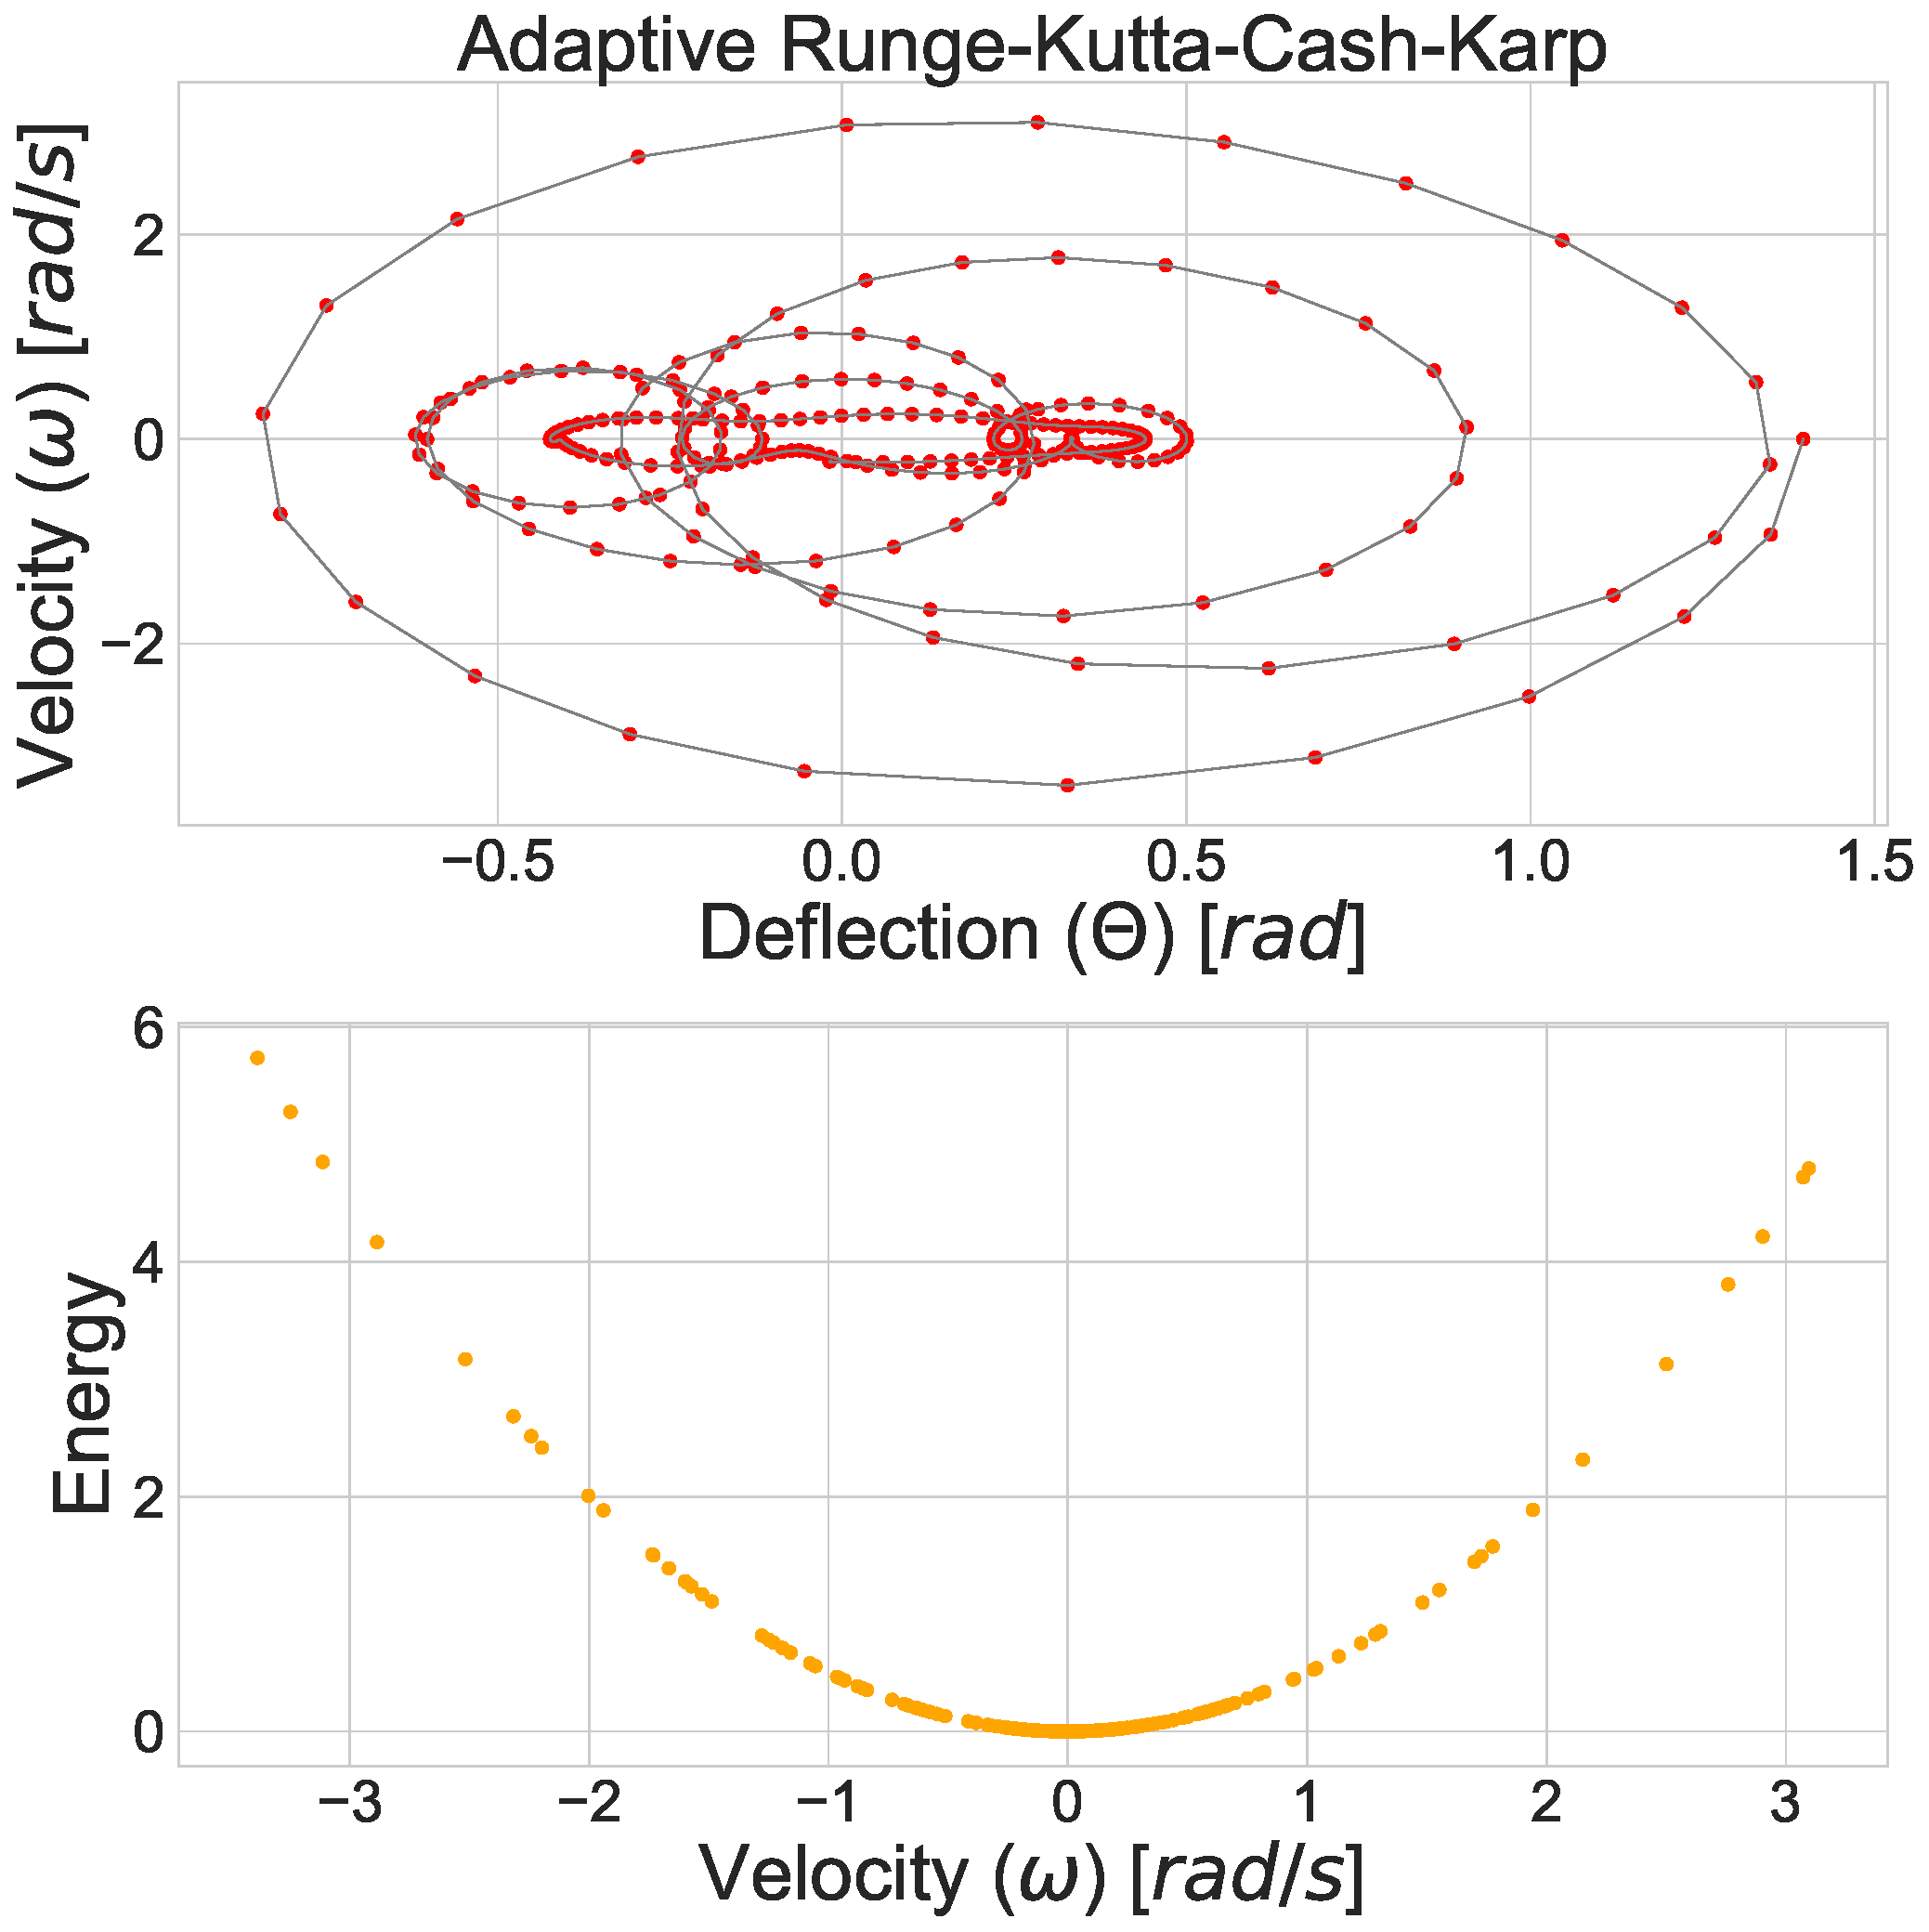
\includegraphics[width=.25\textwidth]{images/phase_energy_adapt_rkck_dampeddriven.pdf}}
\captionof{figure}{Ad. R-K-C-K\\Damp.-Driv.}\label{fig:42}
\hfill
{\centering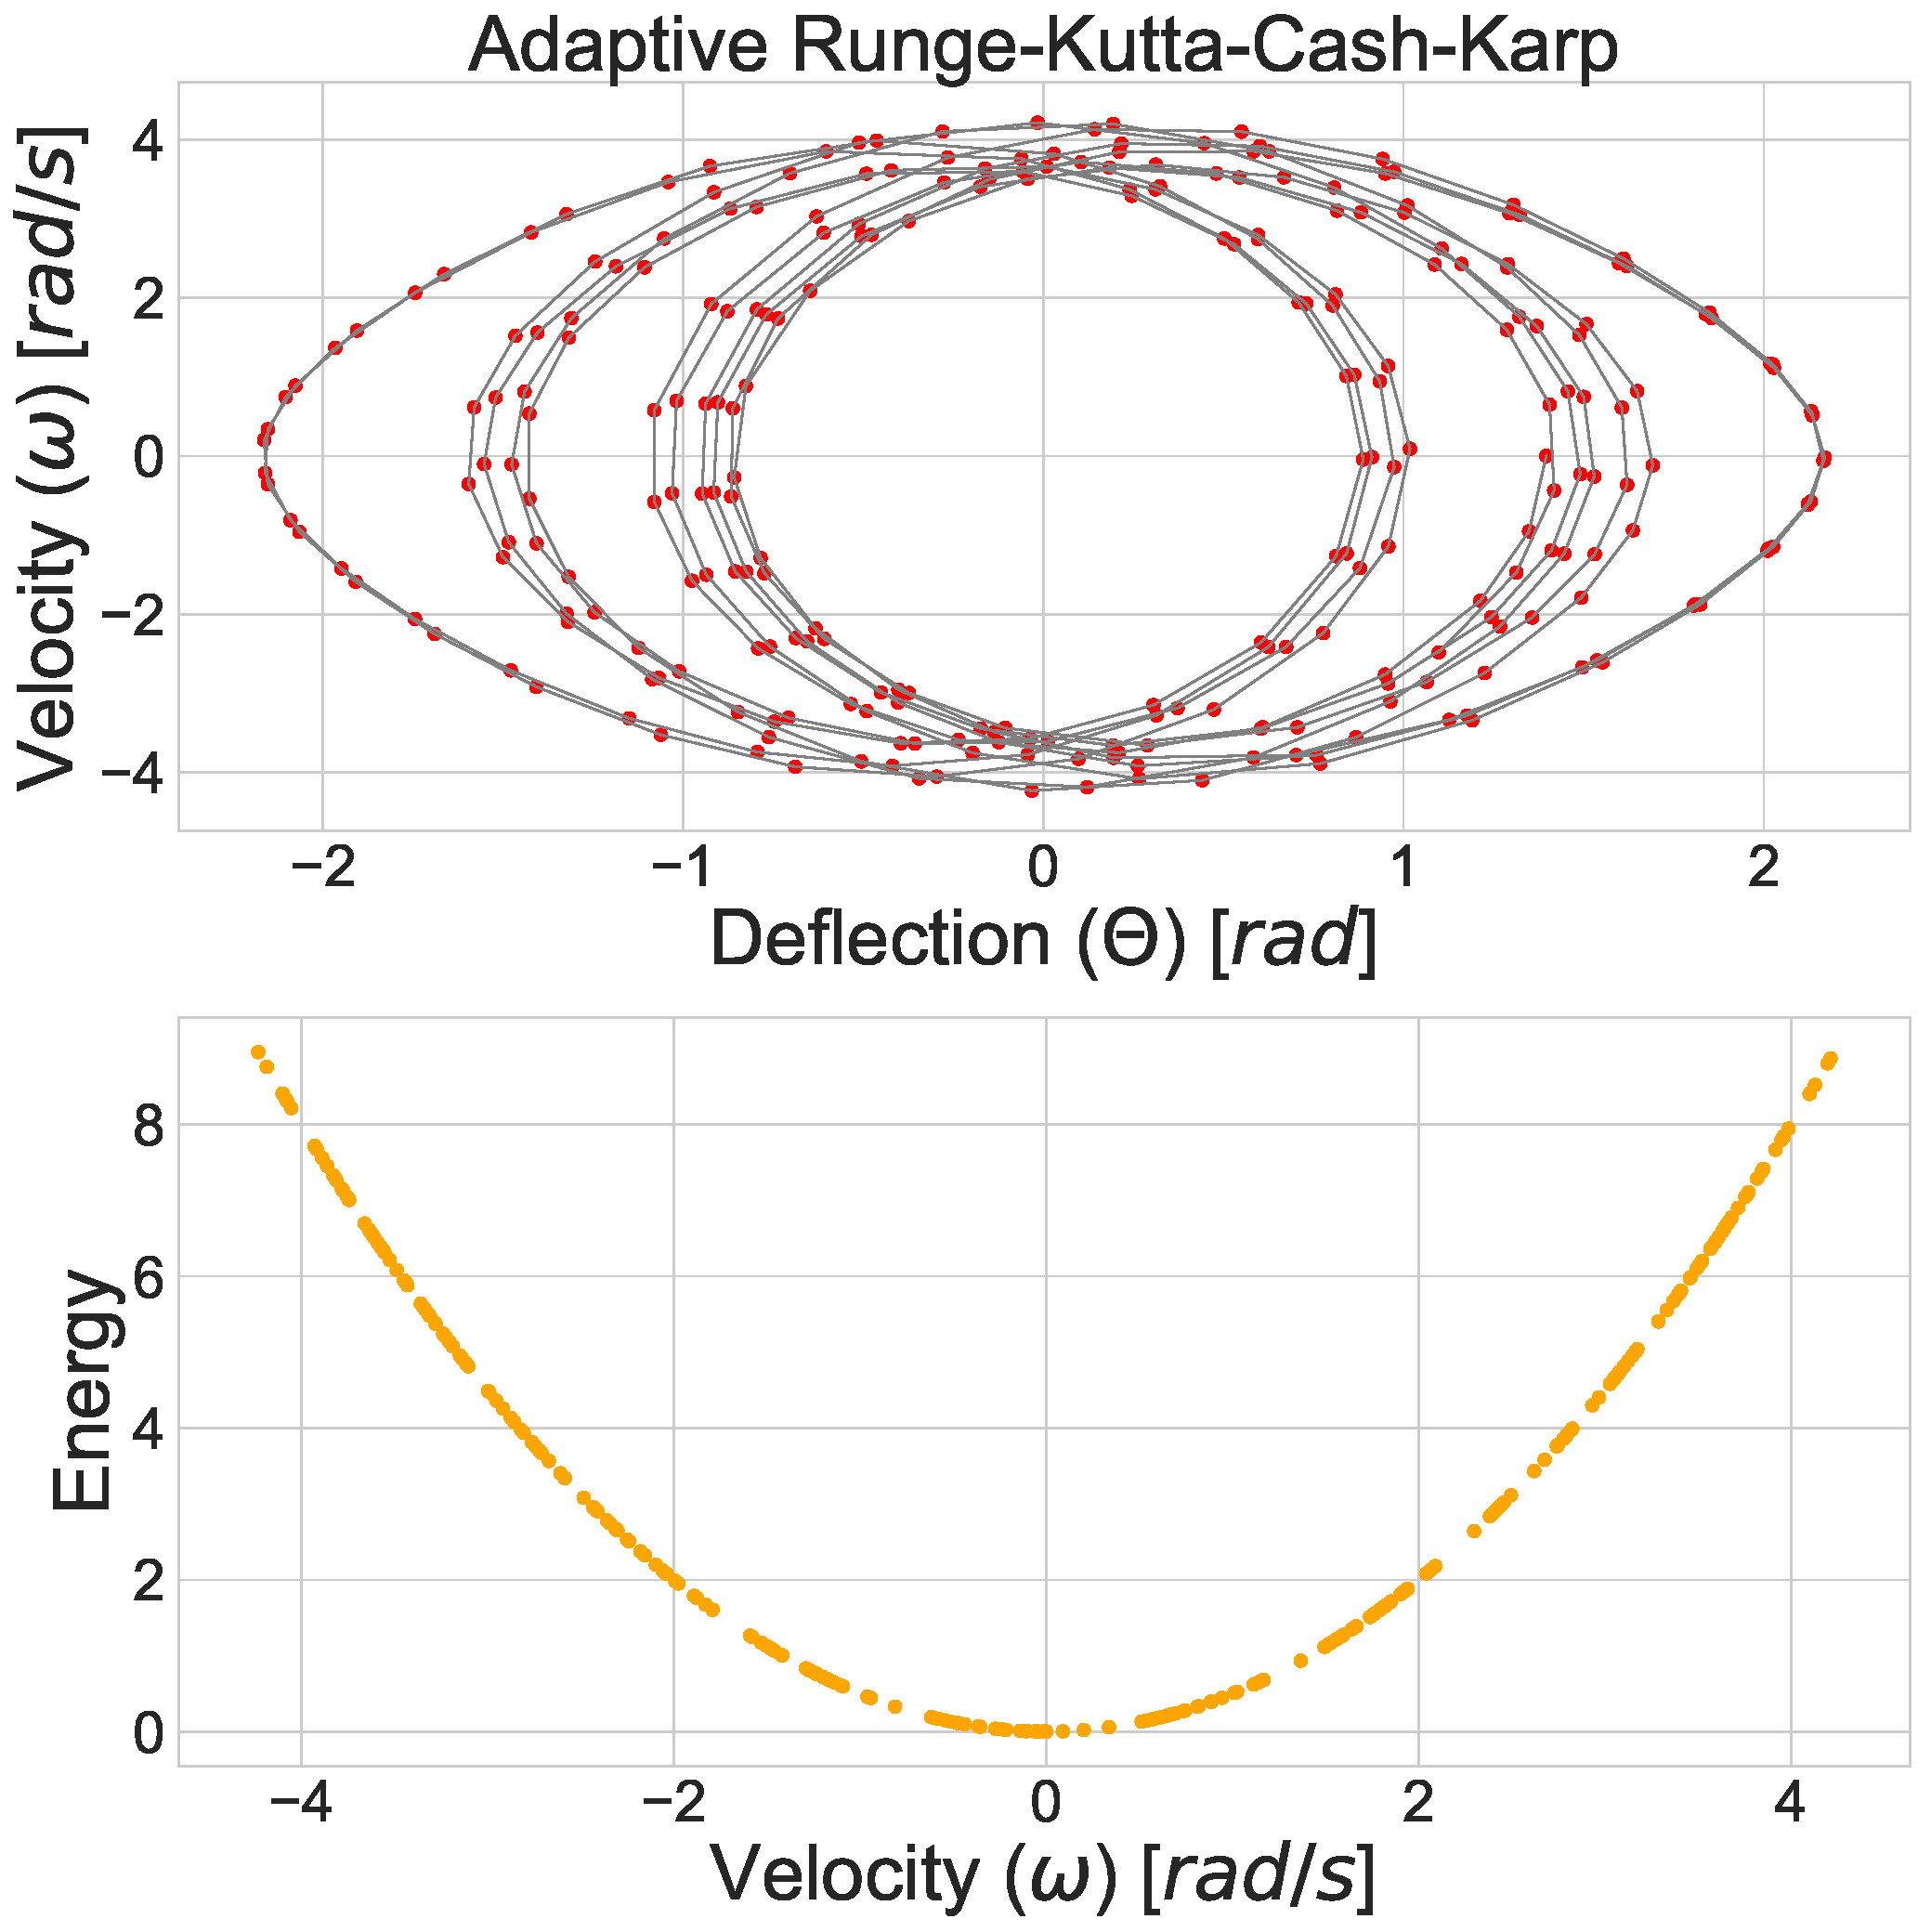
\includegraphics[width=.25\textwidth]{images/phase_energy_adapt_rkck_driven.pdf}}
\captionof{figure}{Ad. R-K-C-K\\Driv.}\label{fig:43}
\hfill

\end{multicols}

\newpage

\begin{multicols}{4}

{\centering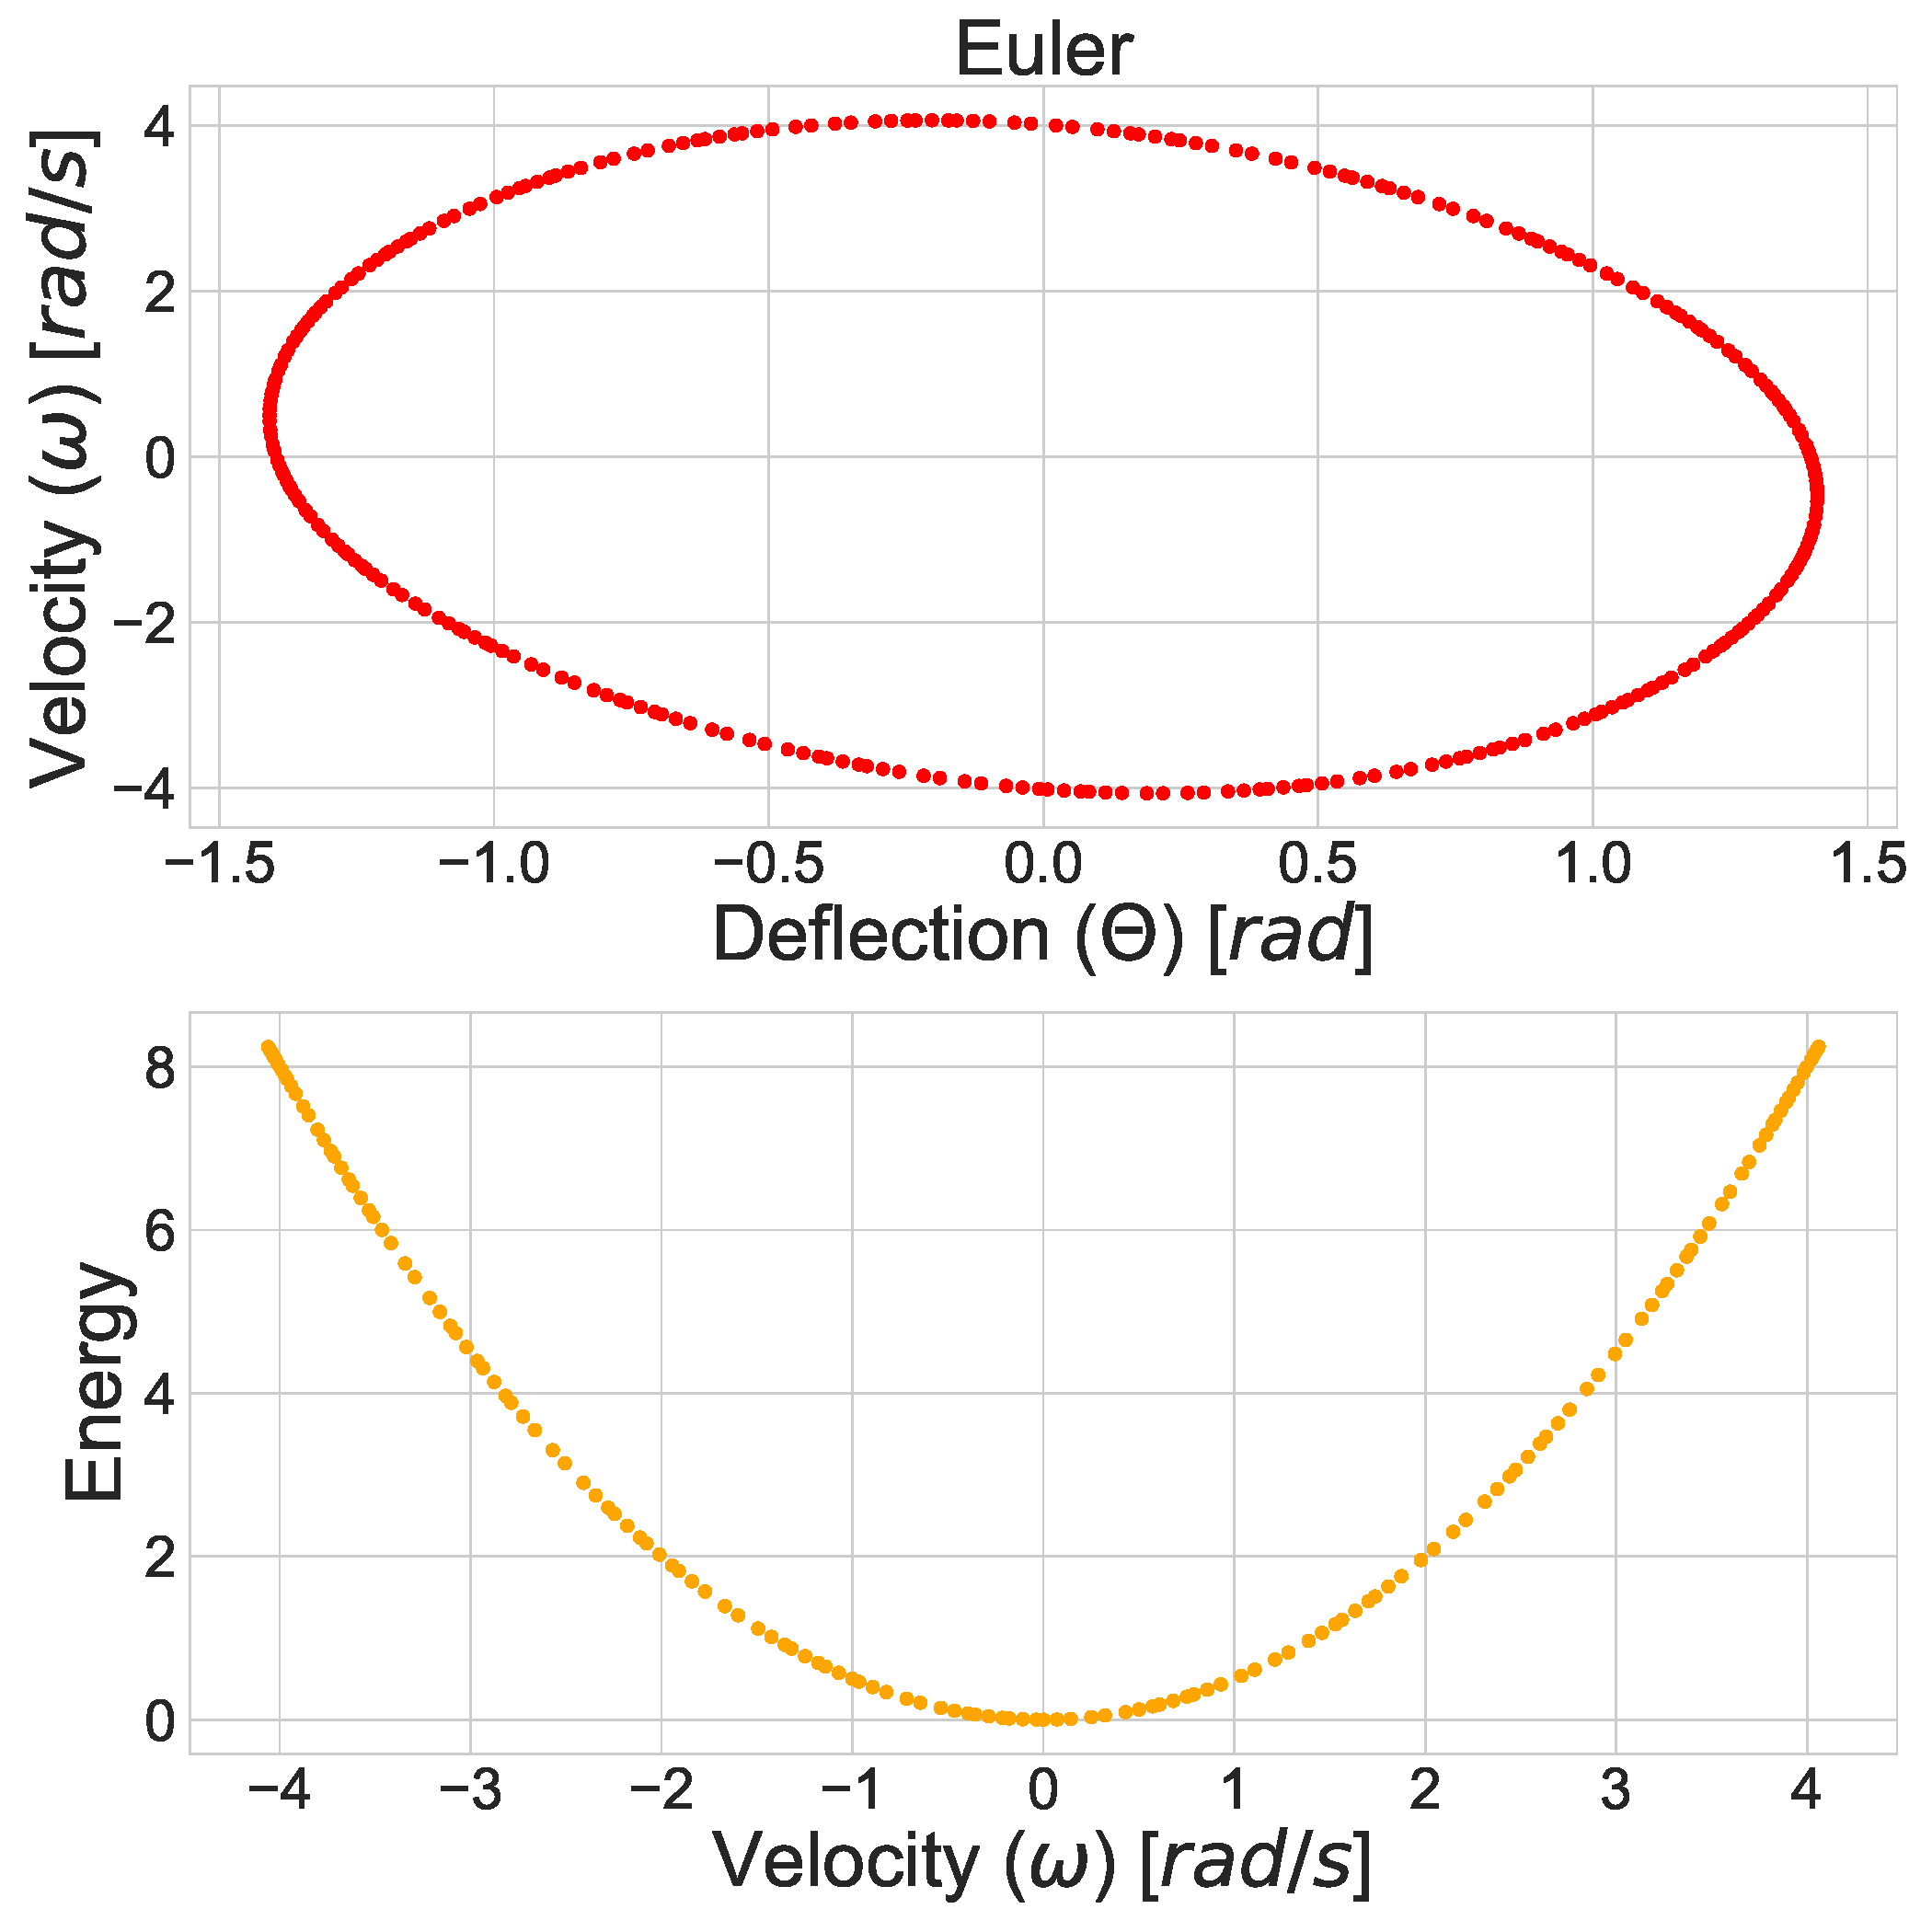
\includegraphics[width=.25\textwidth]{images/phase_energy_euler.pdf}}
\captionof{figure}{Euler\\Mat.}\label{fig:44}
\hfill
{\centering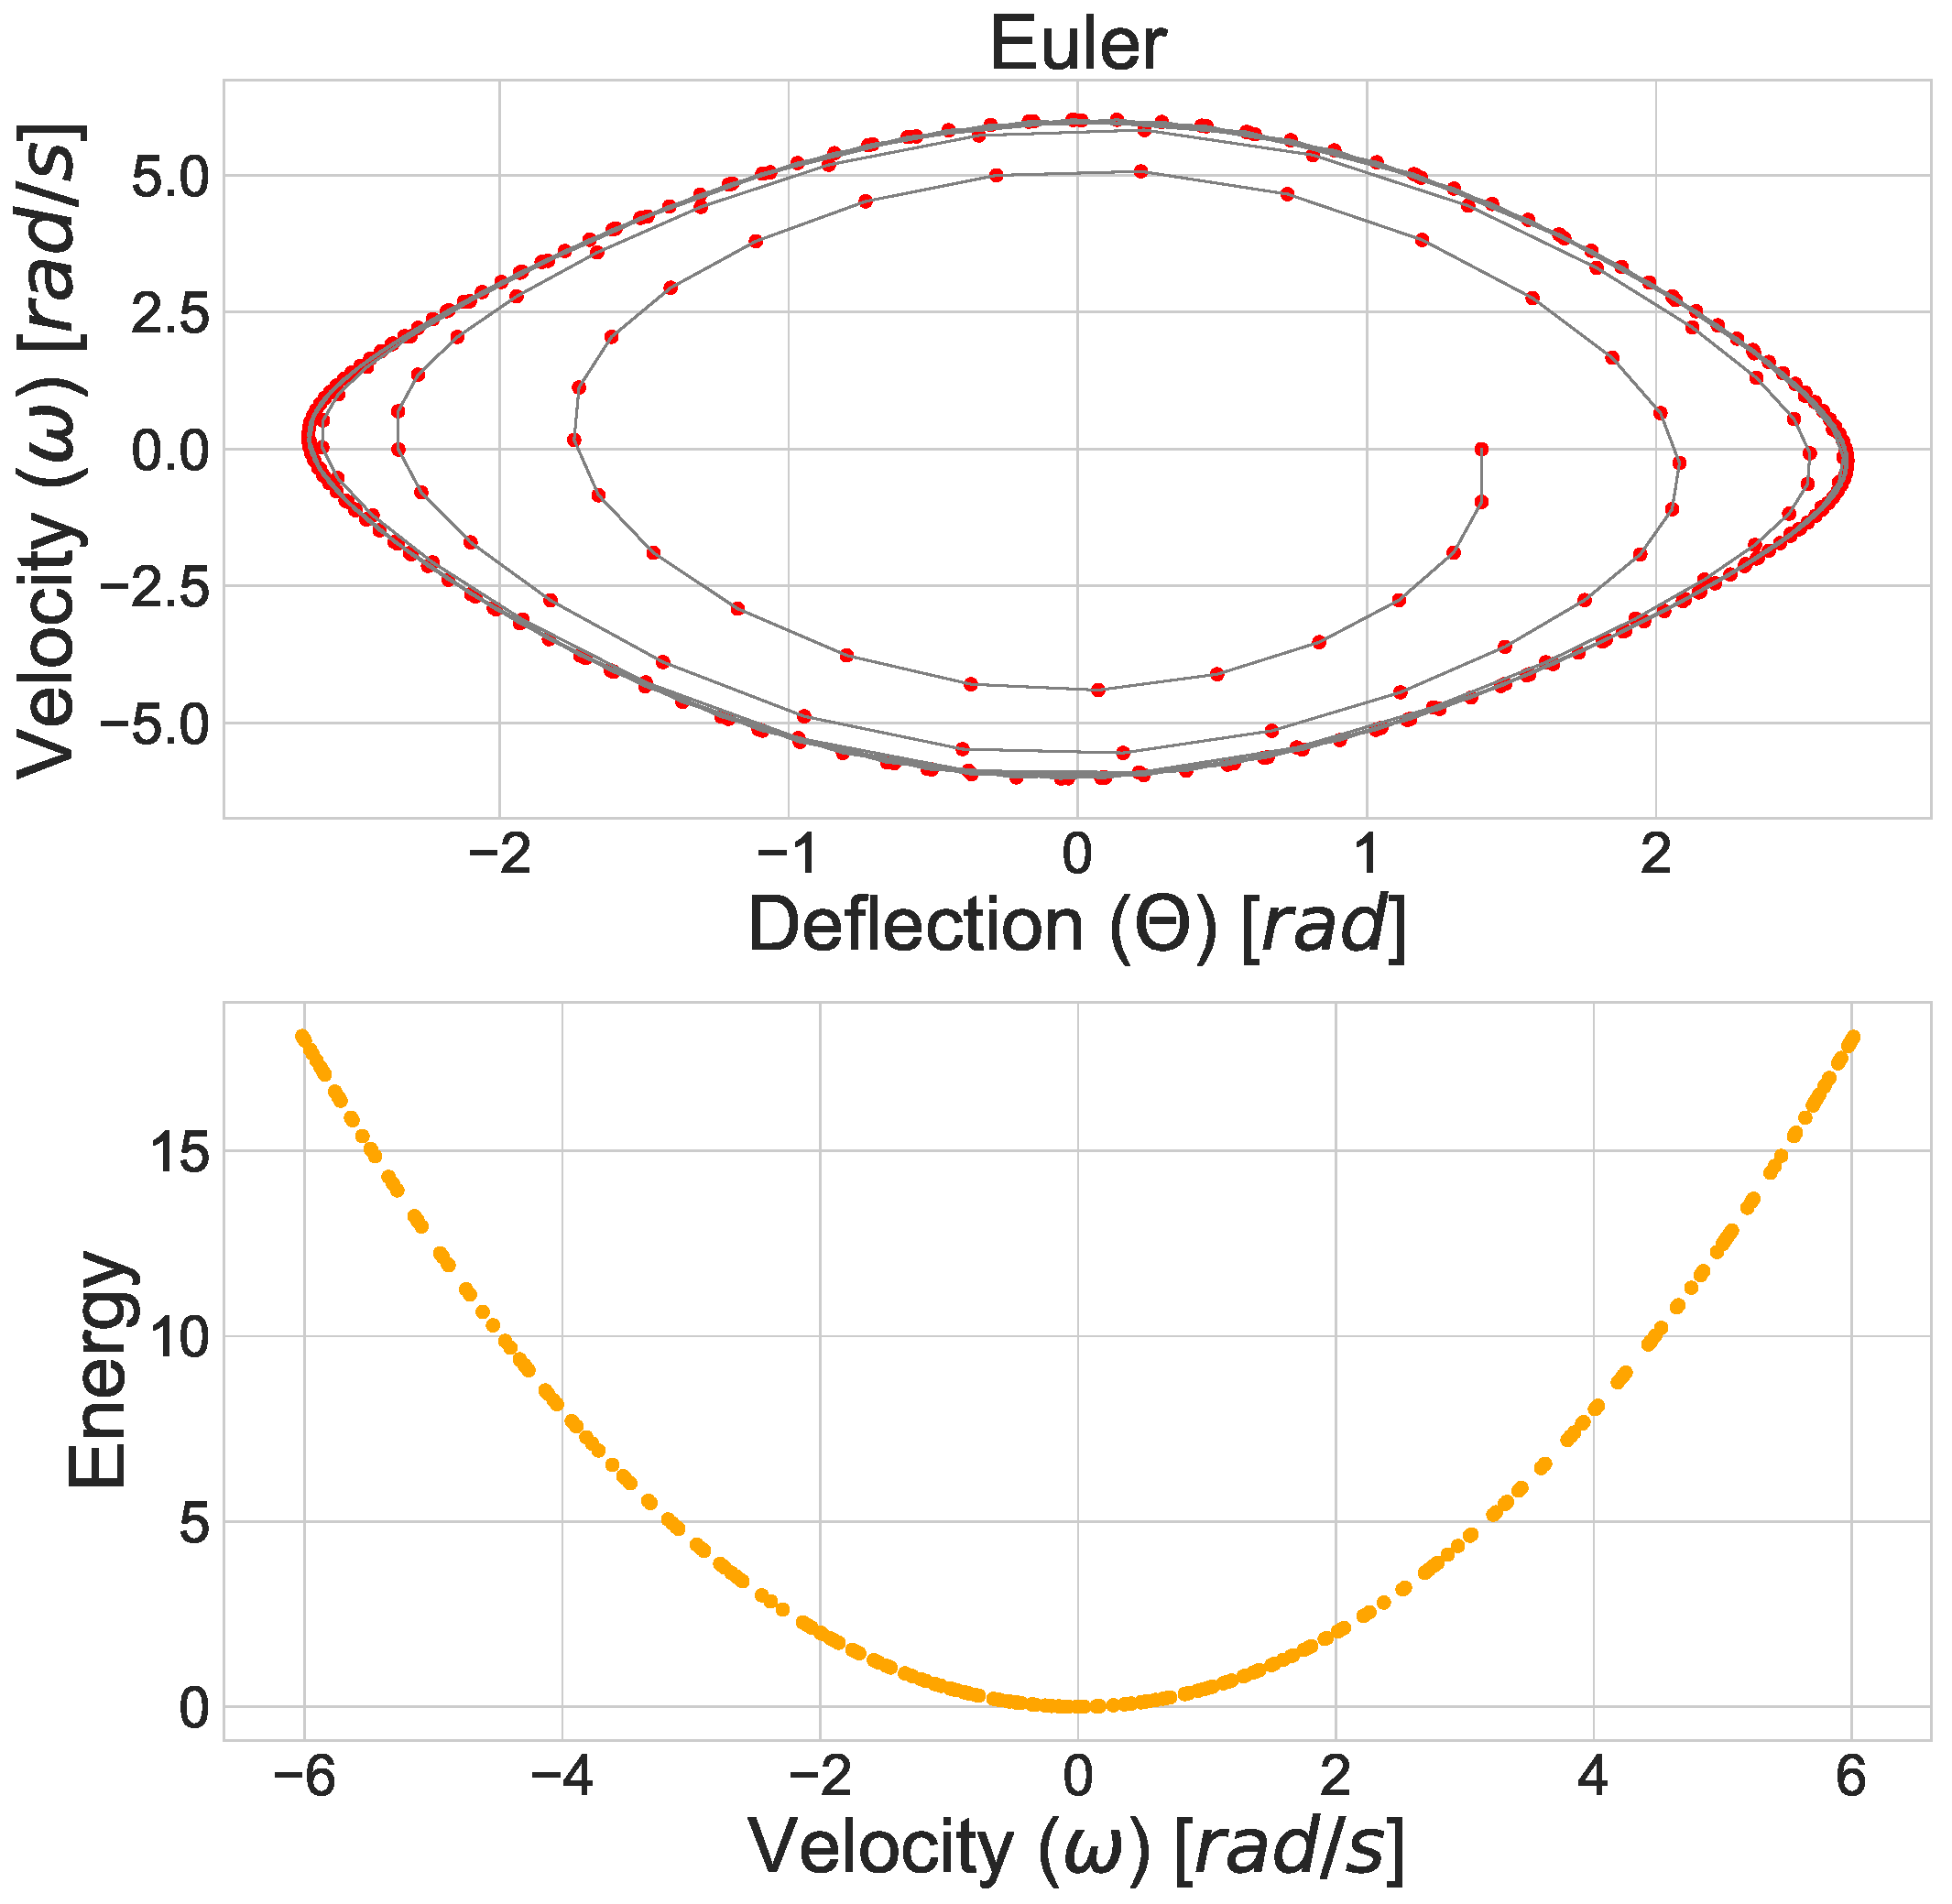
\includegraphics[width=.25\textwidth]{images/phase_energy_euler_damped.pdf}}
\captionof{figure}{Euler\\Damp.}\label{fig:45}
\hfill
{\centering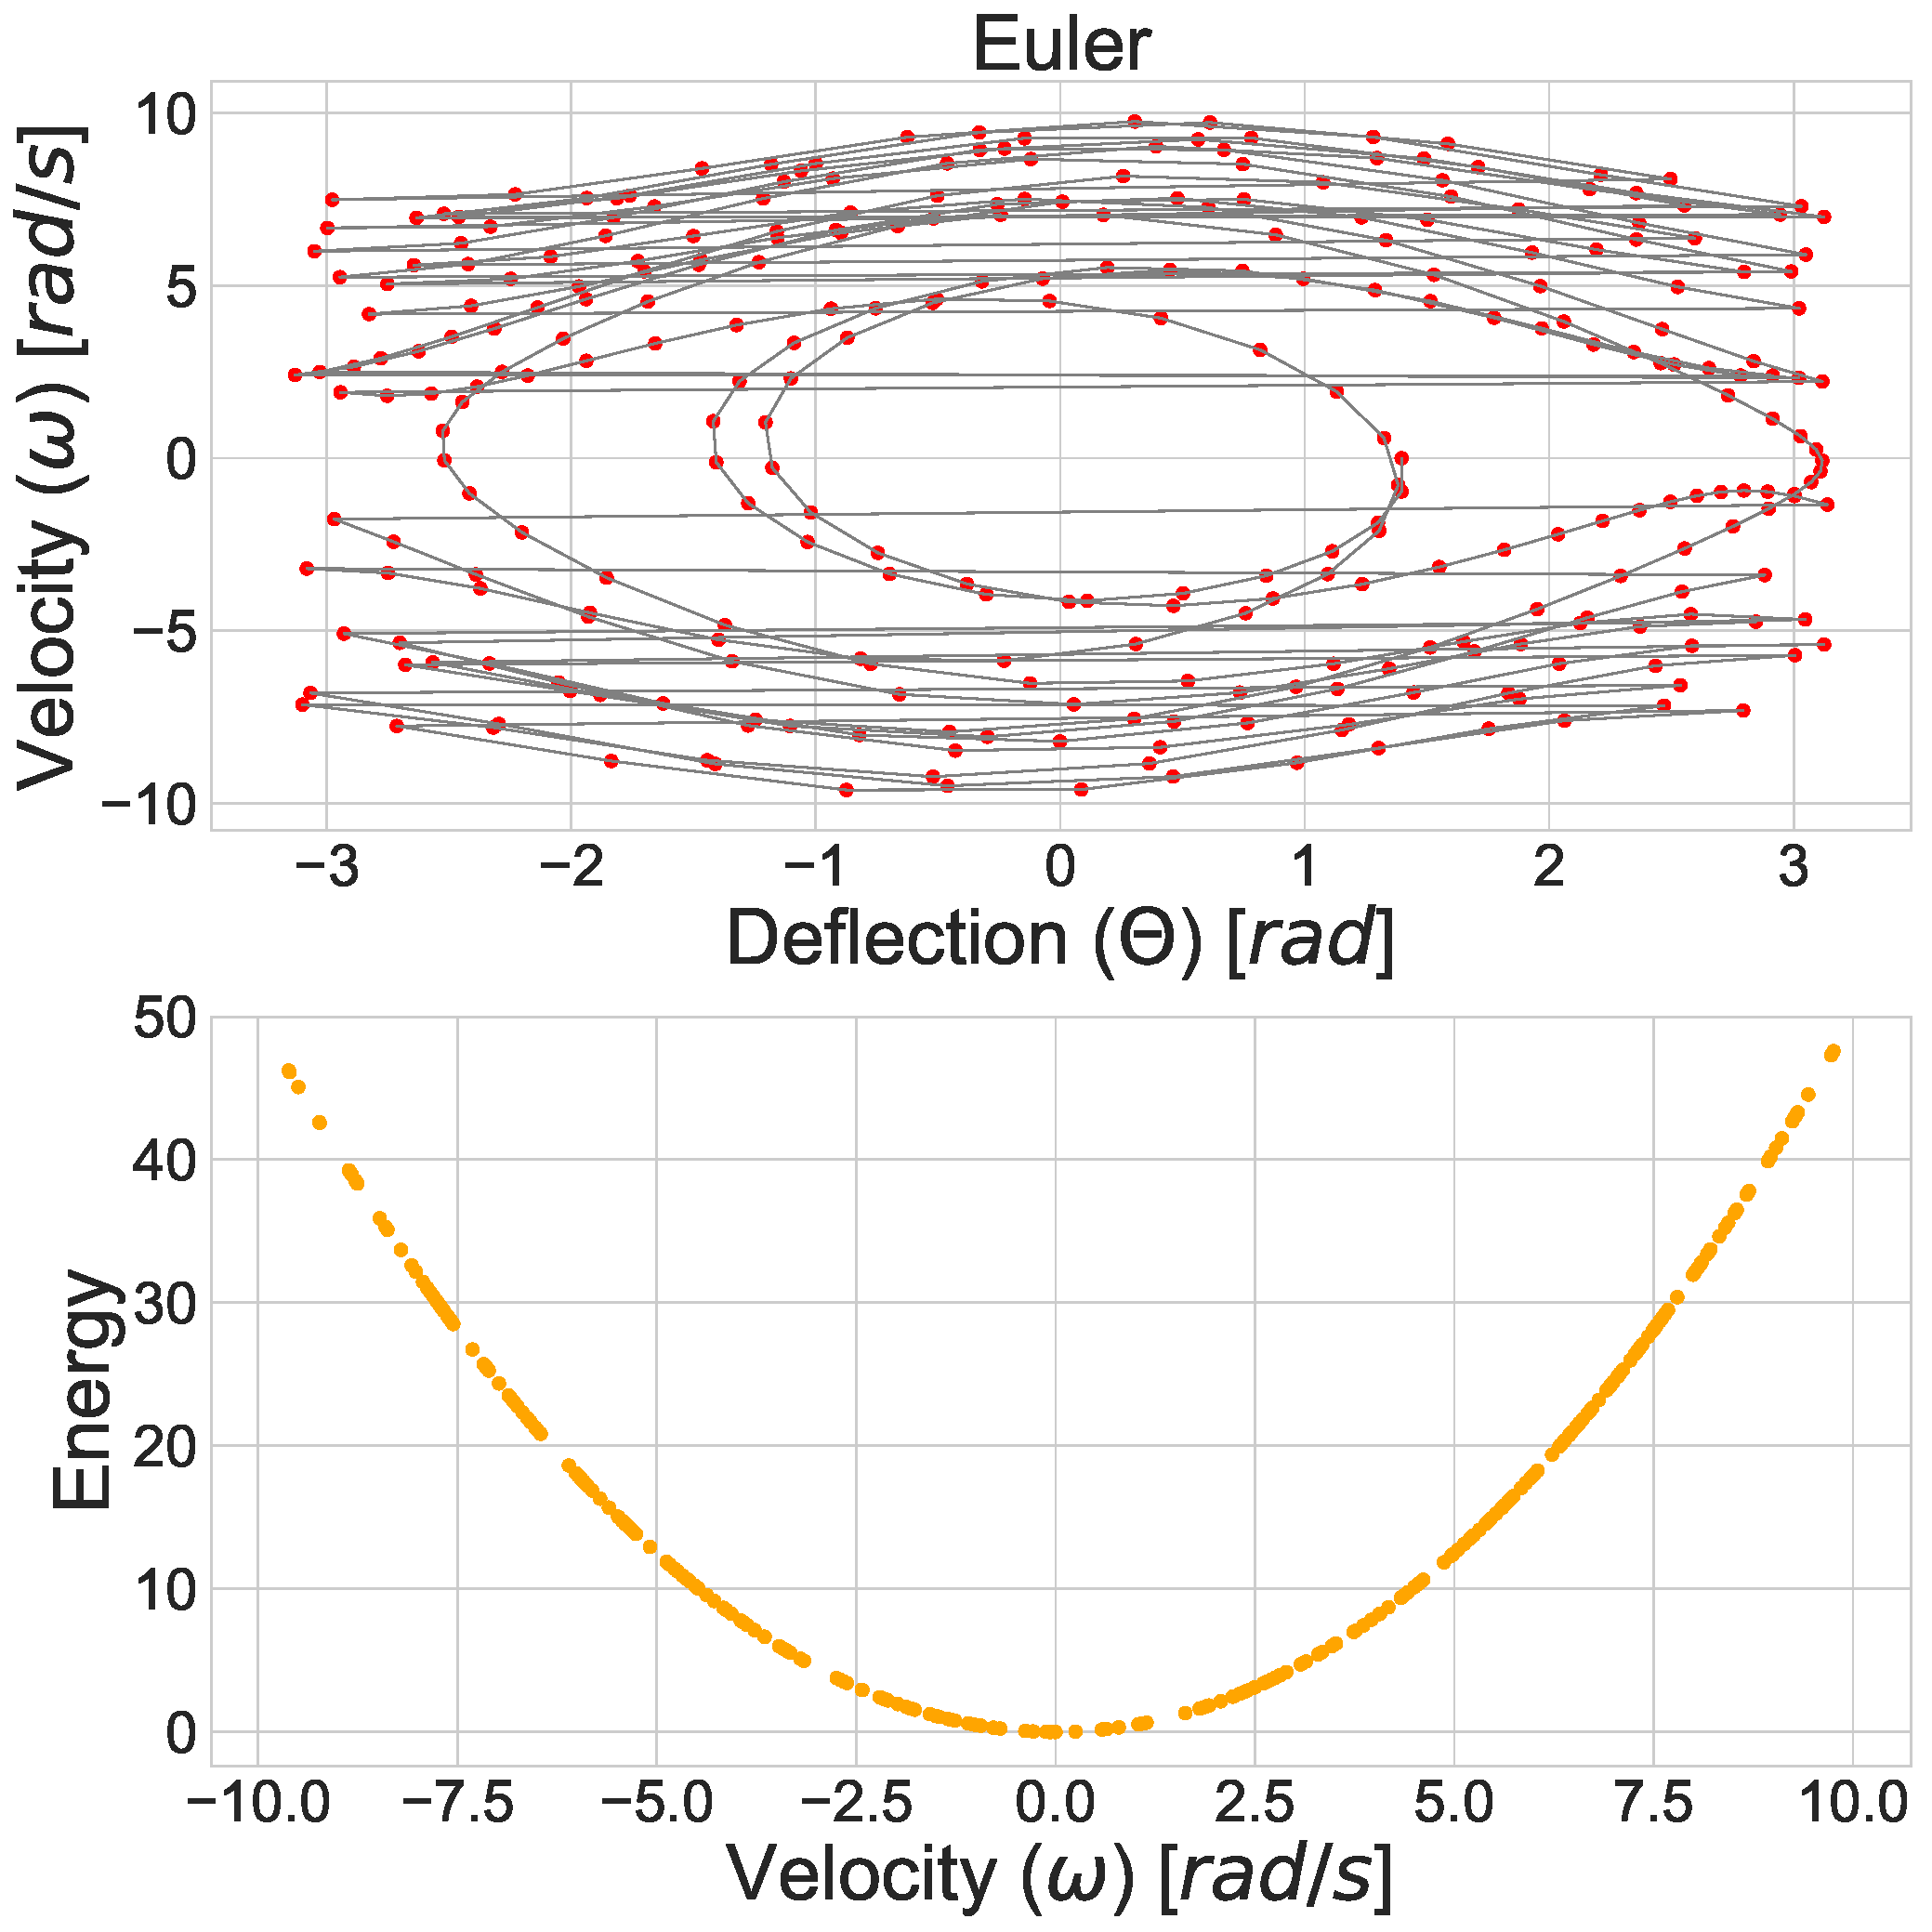
\includegraphics[width=.25\textwidth]{images/phase_energy_euler_dampeddriven.pdf}}
\captionof{figure}{Euler\\Damp.-Driv.}\label{fig:46}
\hfill
{\centering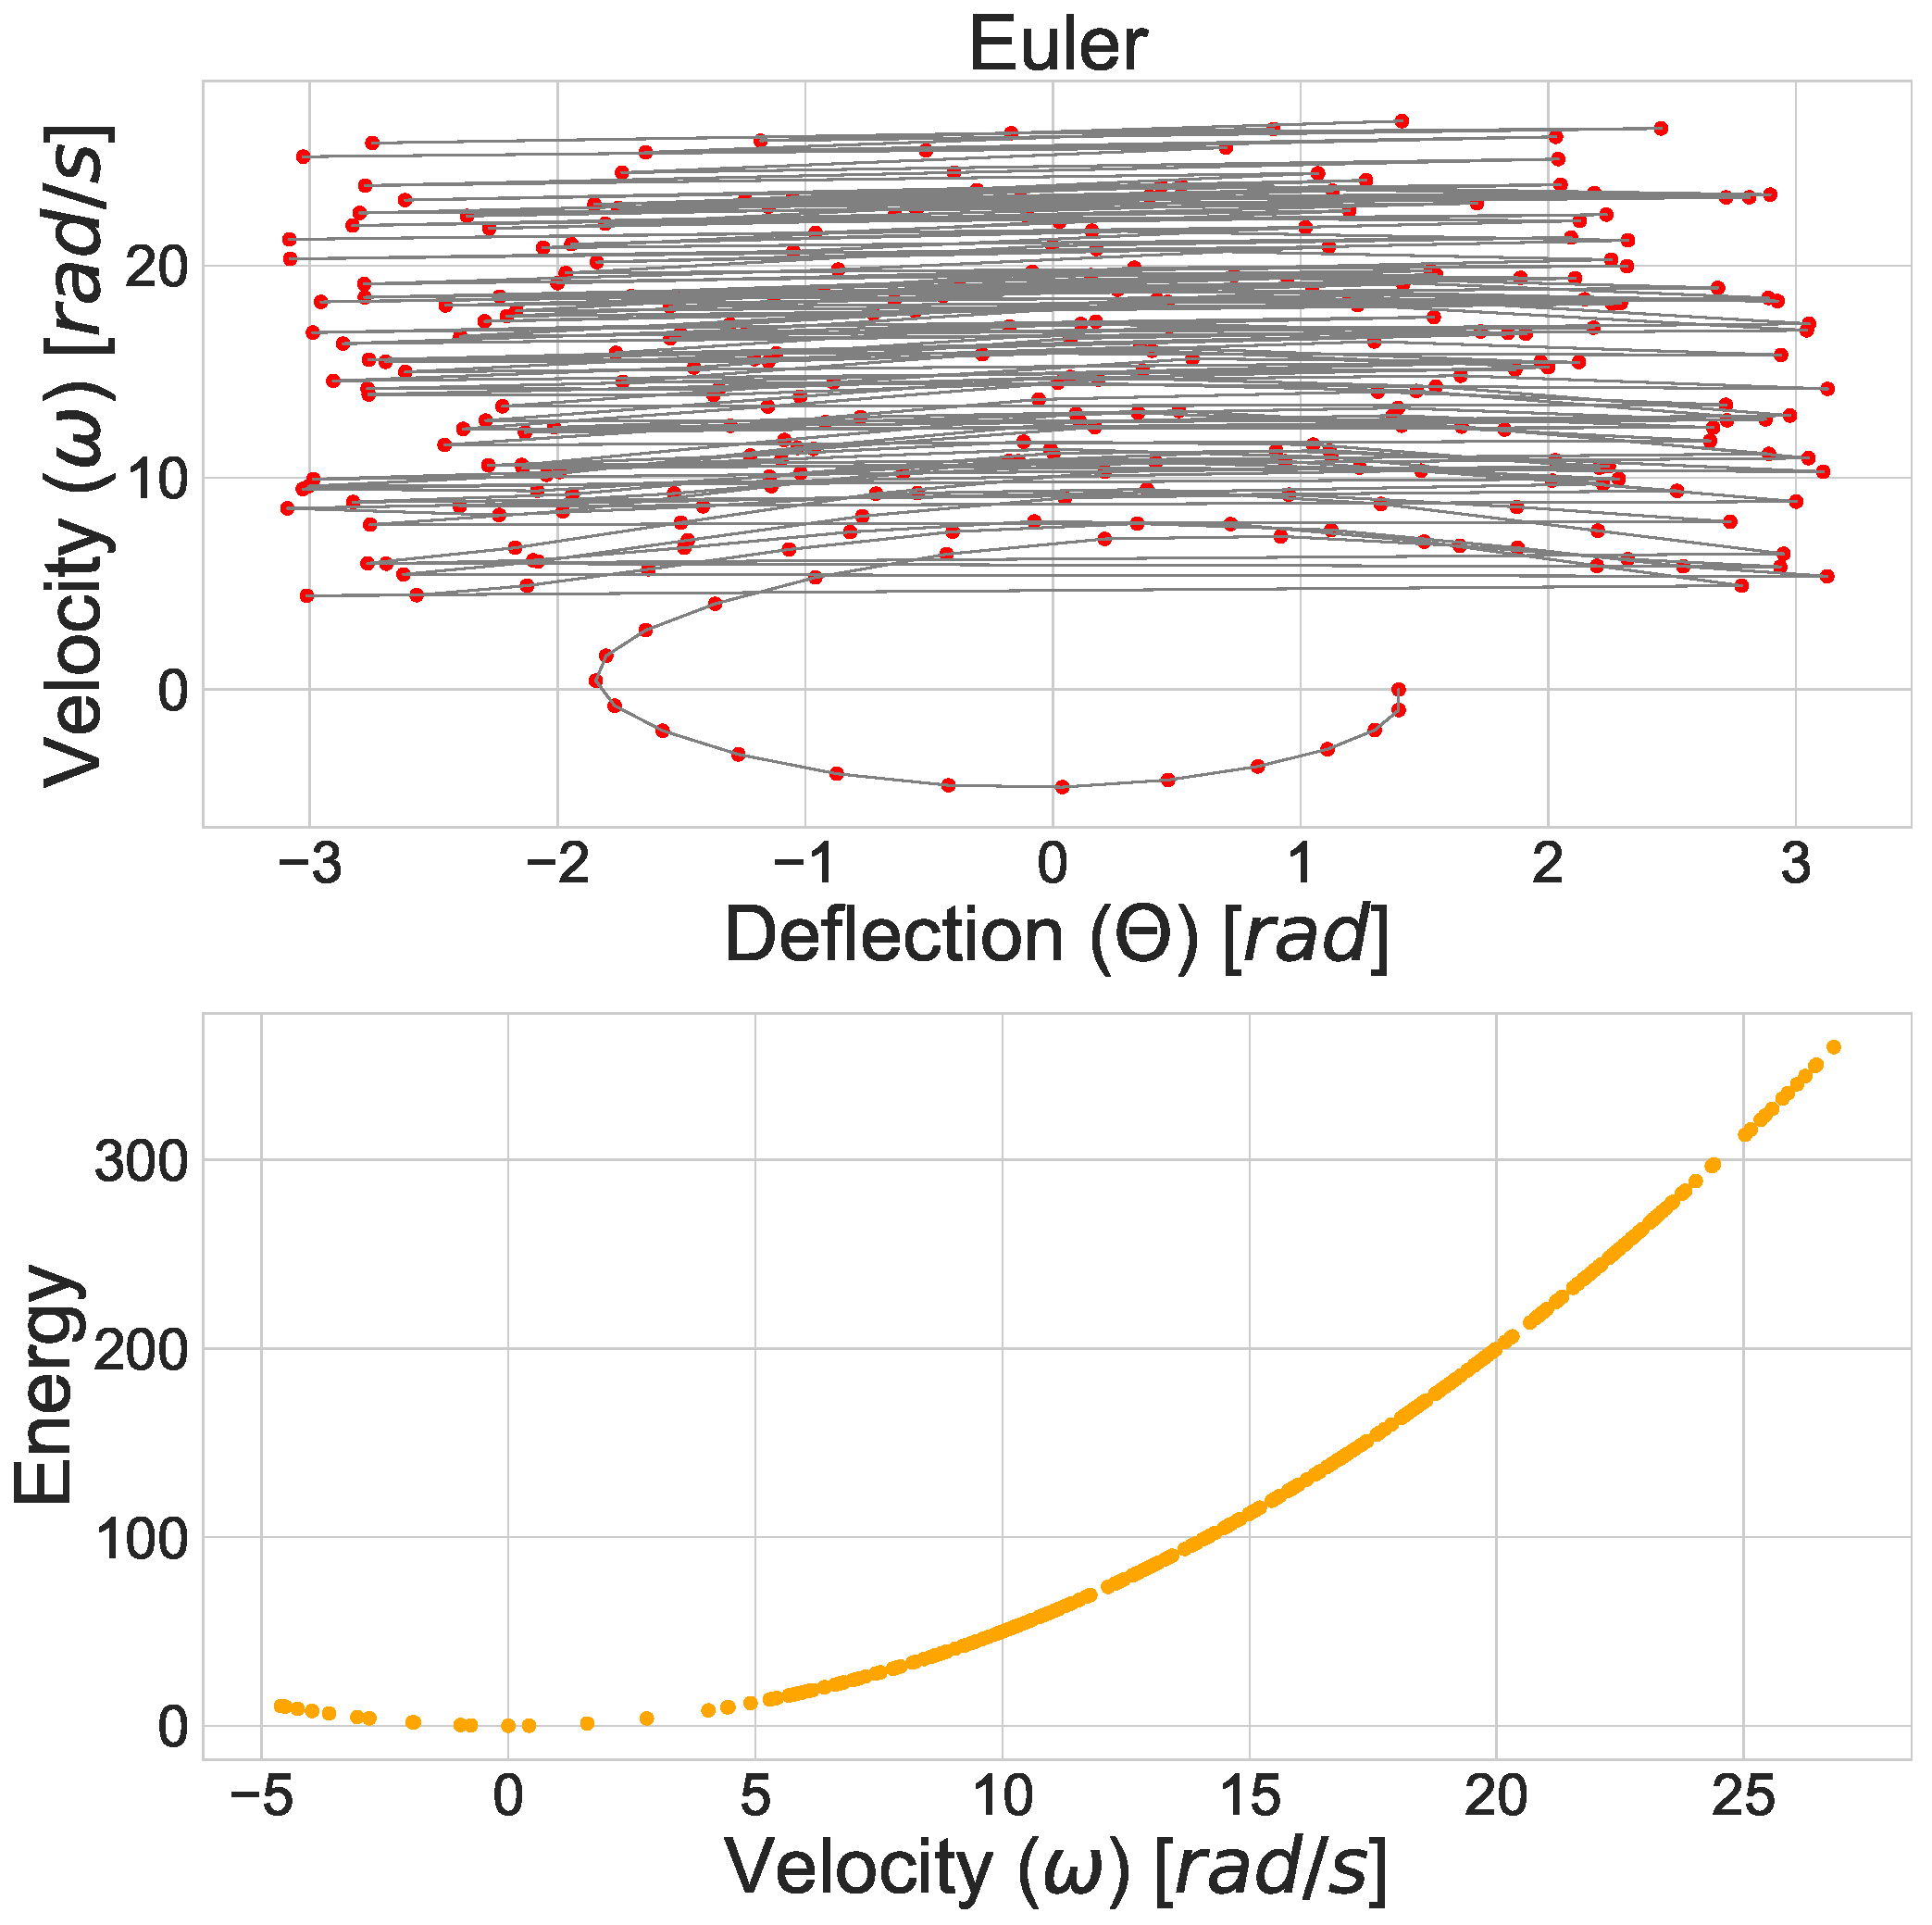
\includegraphics[width=.25\textwidth]{images/phase_energy_euler_driven.pdf}}
\captionof{figure}{Euler\\Driv.}\label{fig:47}
\hfill

\end{multicols}
\begin{multicols}{4}

{\centering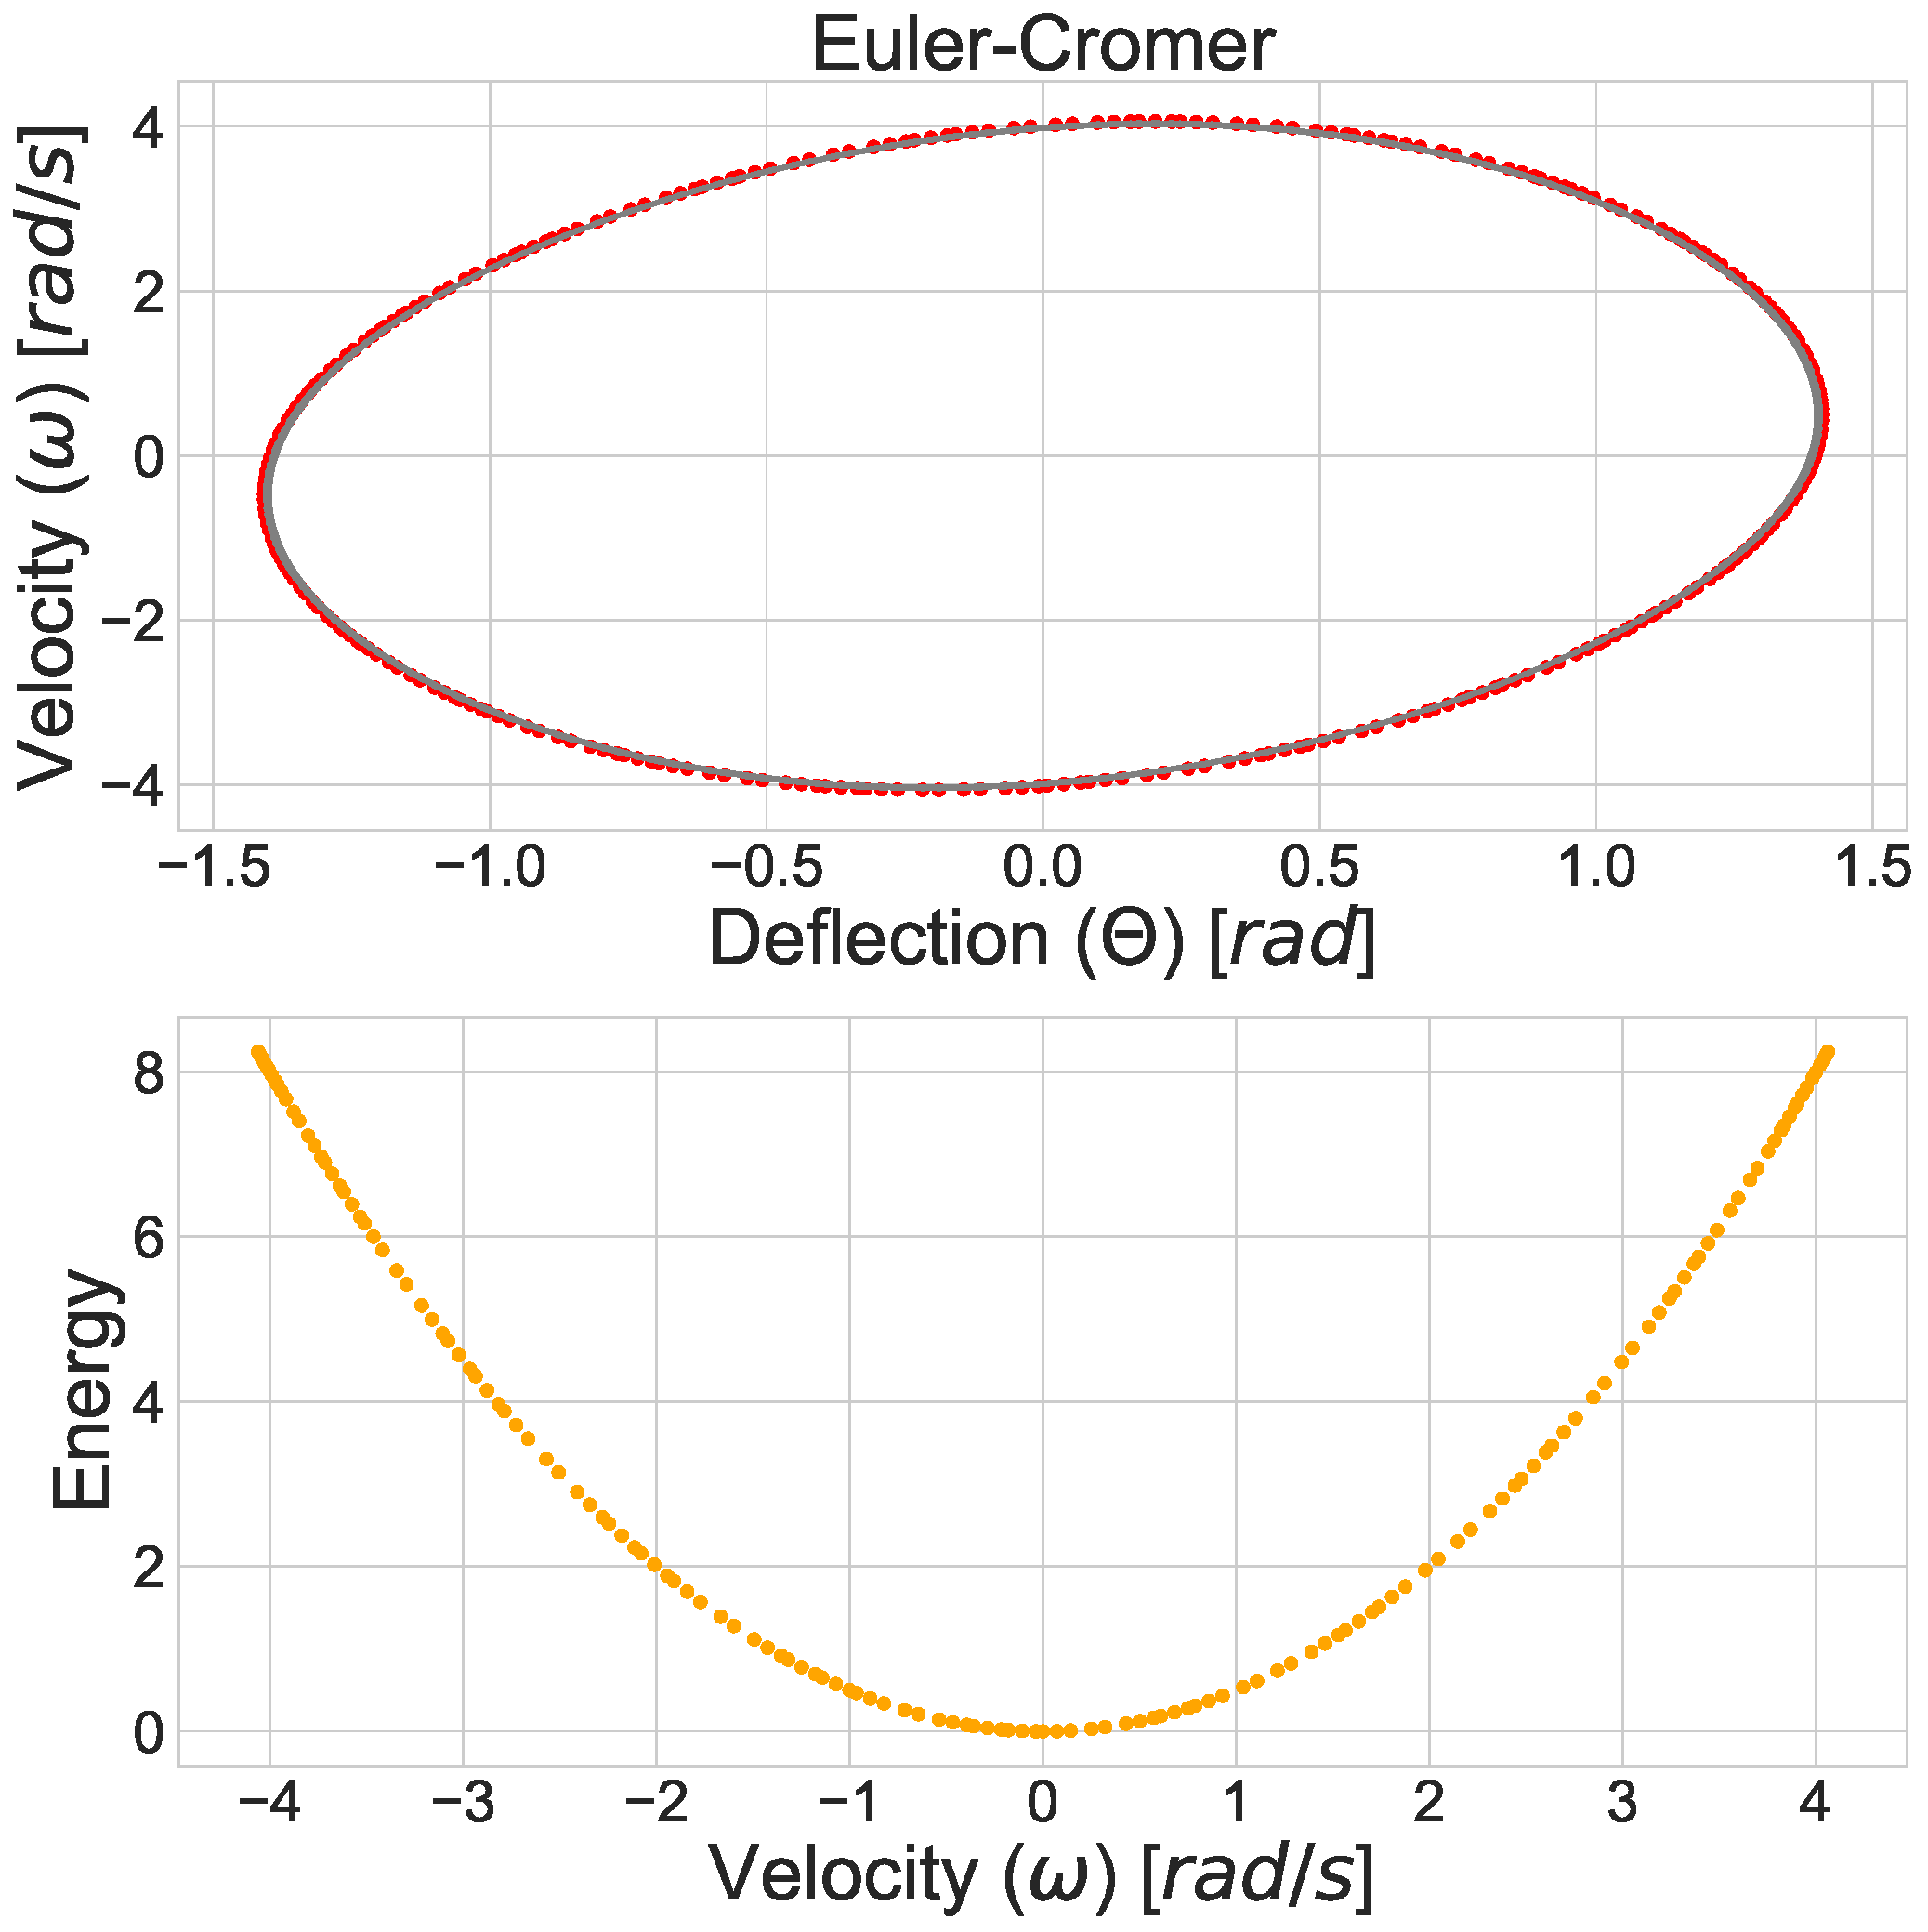
\includegraphics[width=.25\textwidth]{images/phase_energy_eulercromer.pdf}}
\captionof{figure}{Euler-Cromer\\Mat.}\label{fig:48}
\hfill
{\centering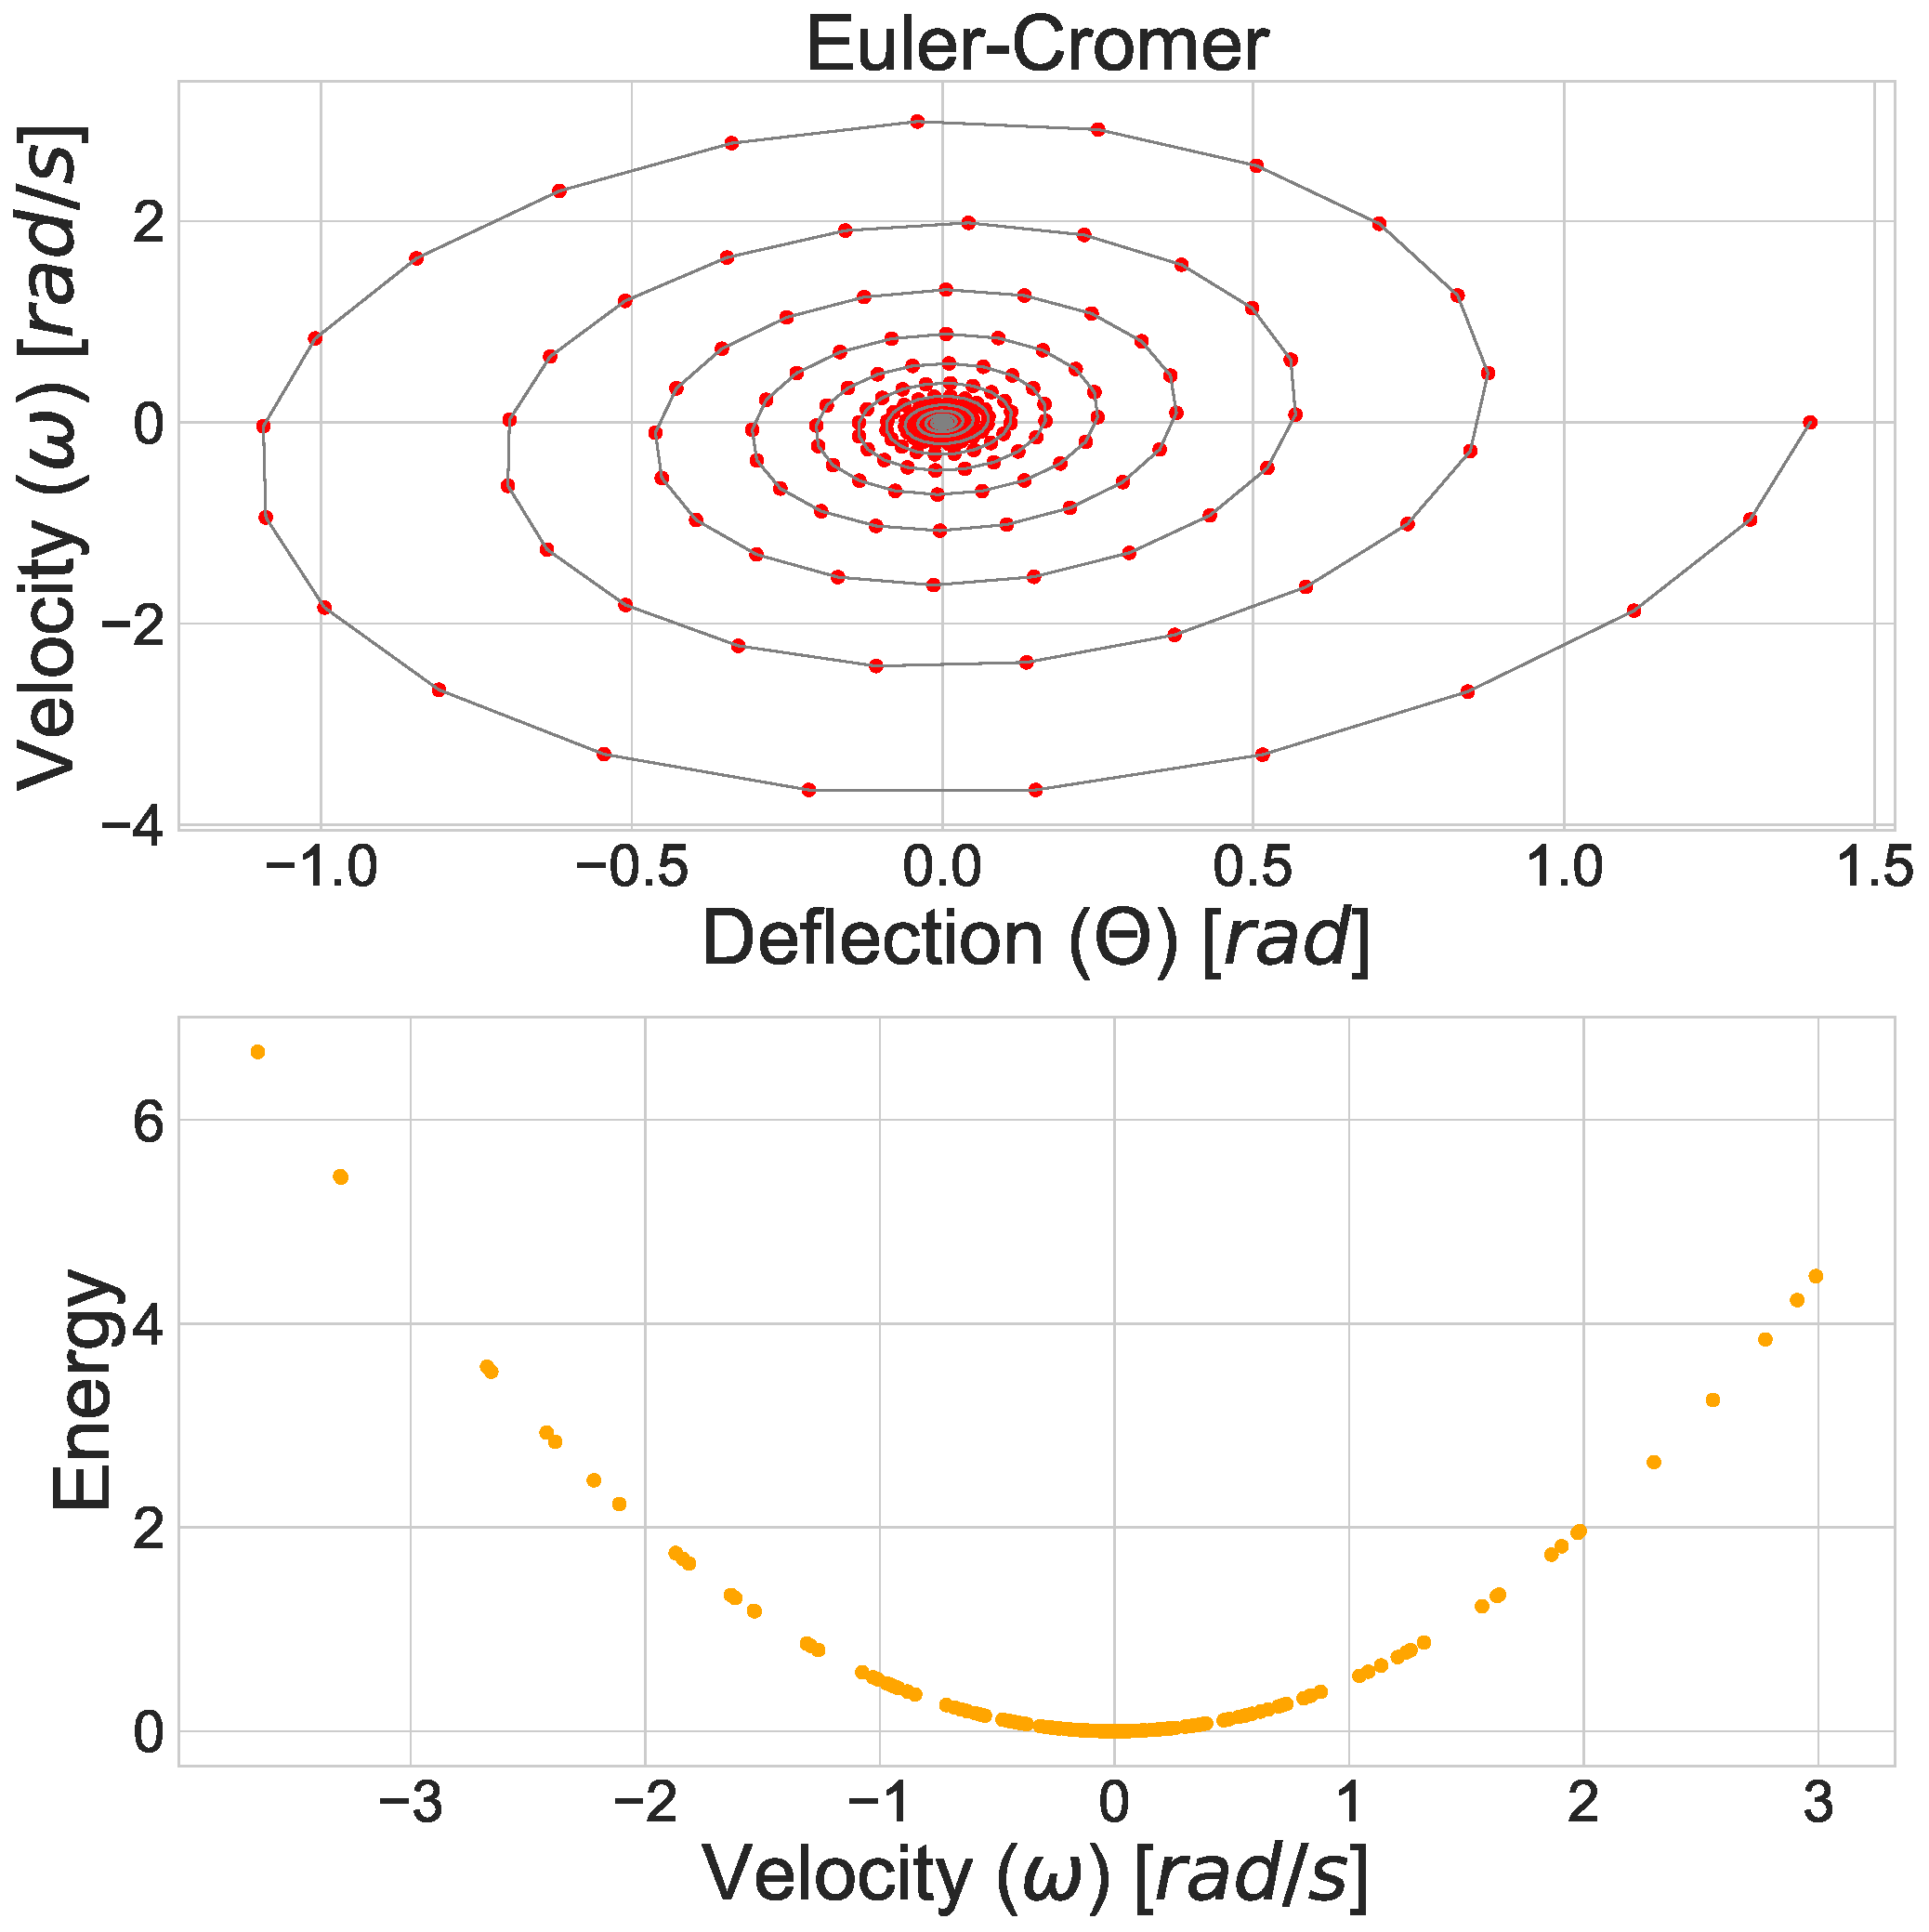
\includegraphics[width=.25\textwidth]{images/phase_energy_eulercromer_damped.pdf}}
\captionof{figure}{Euler-Cromer\\Damp.}\label{fig:49}
\hfill
{\centering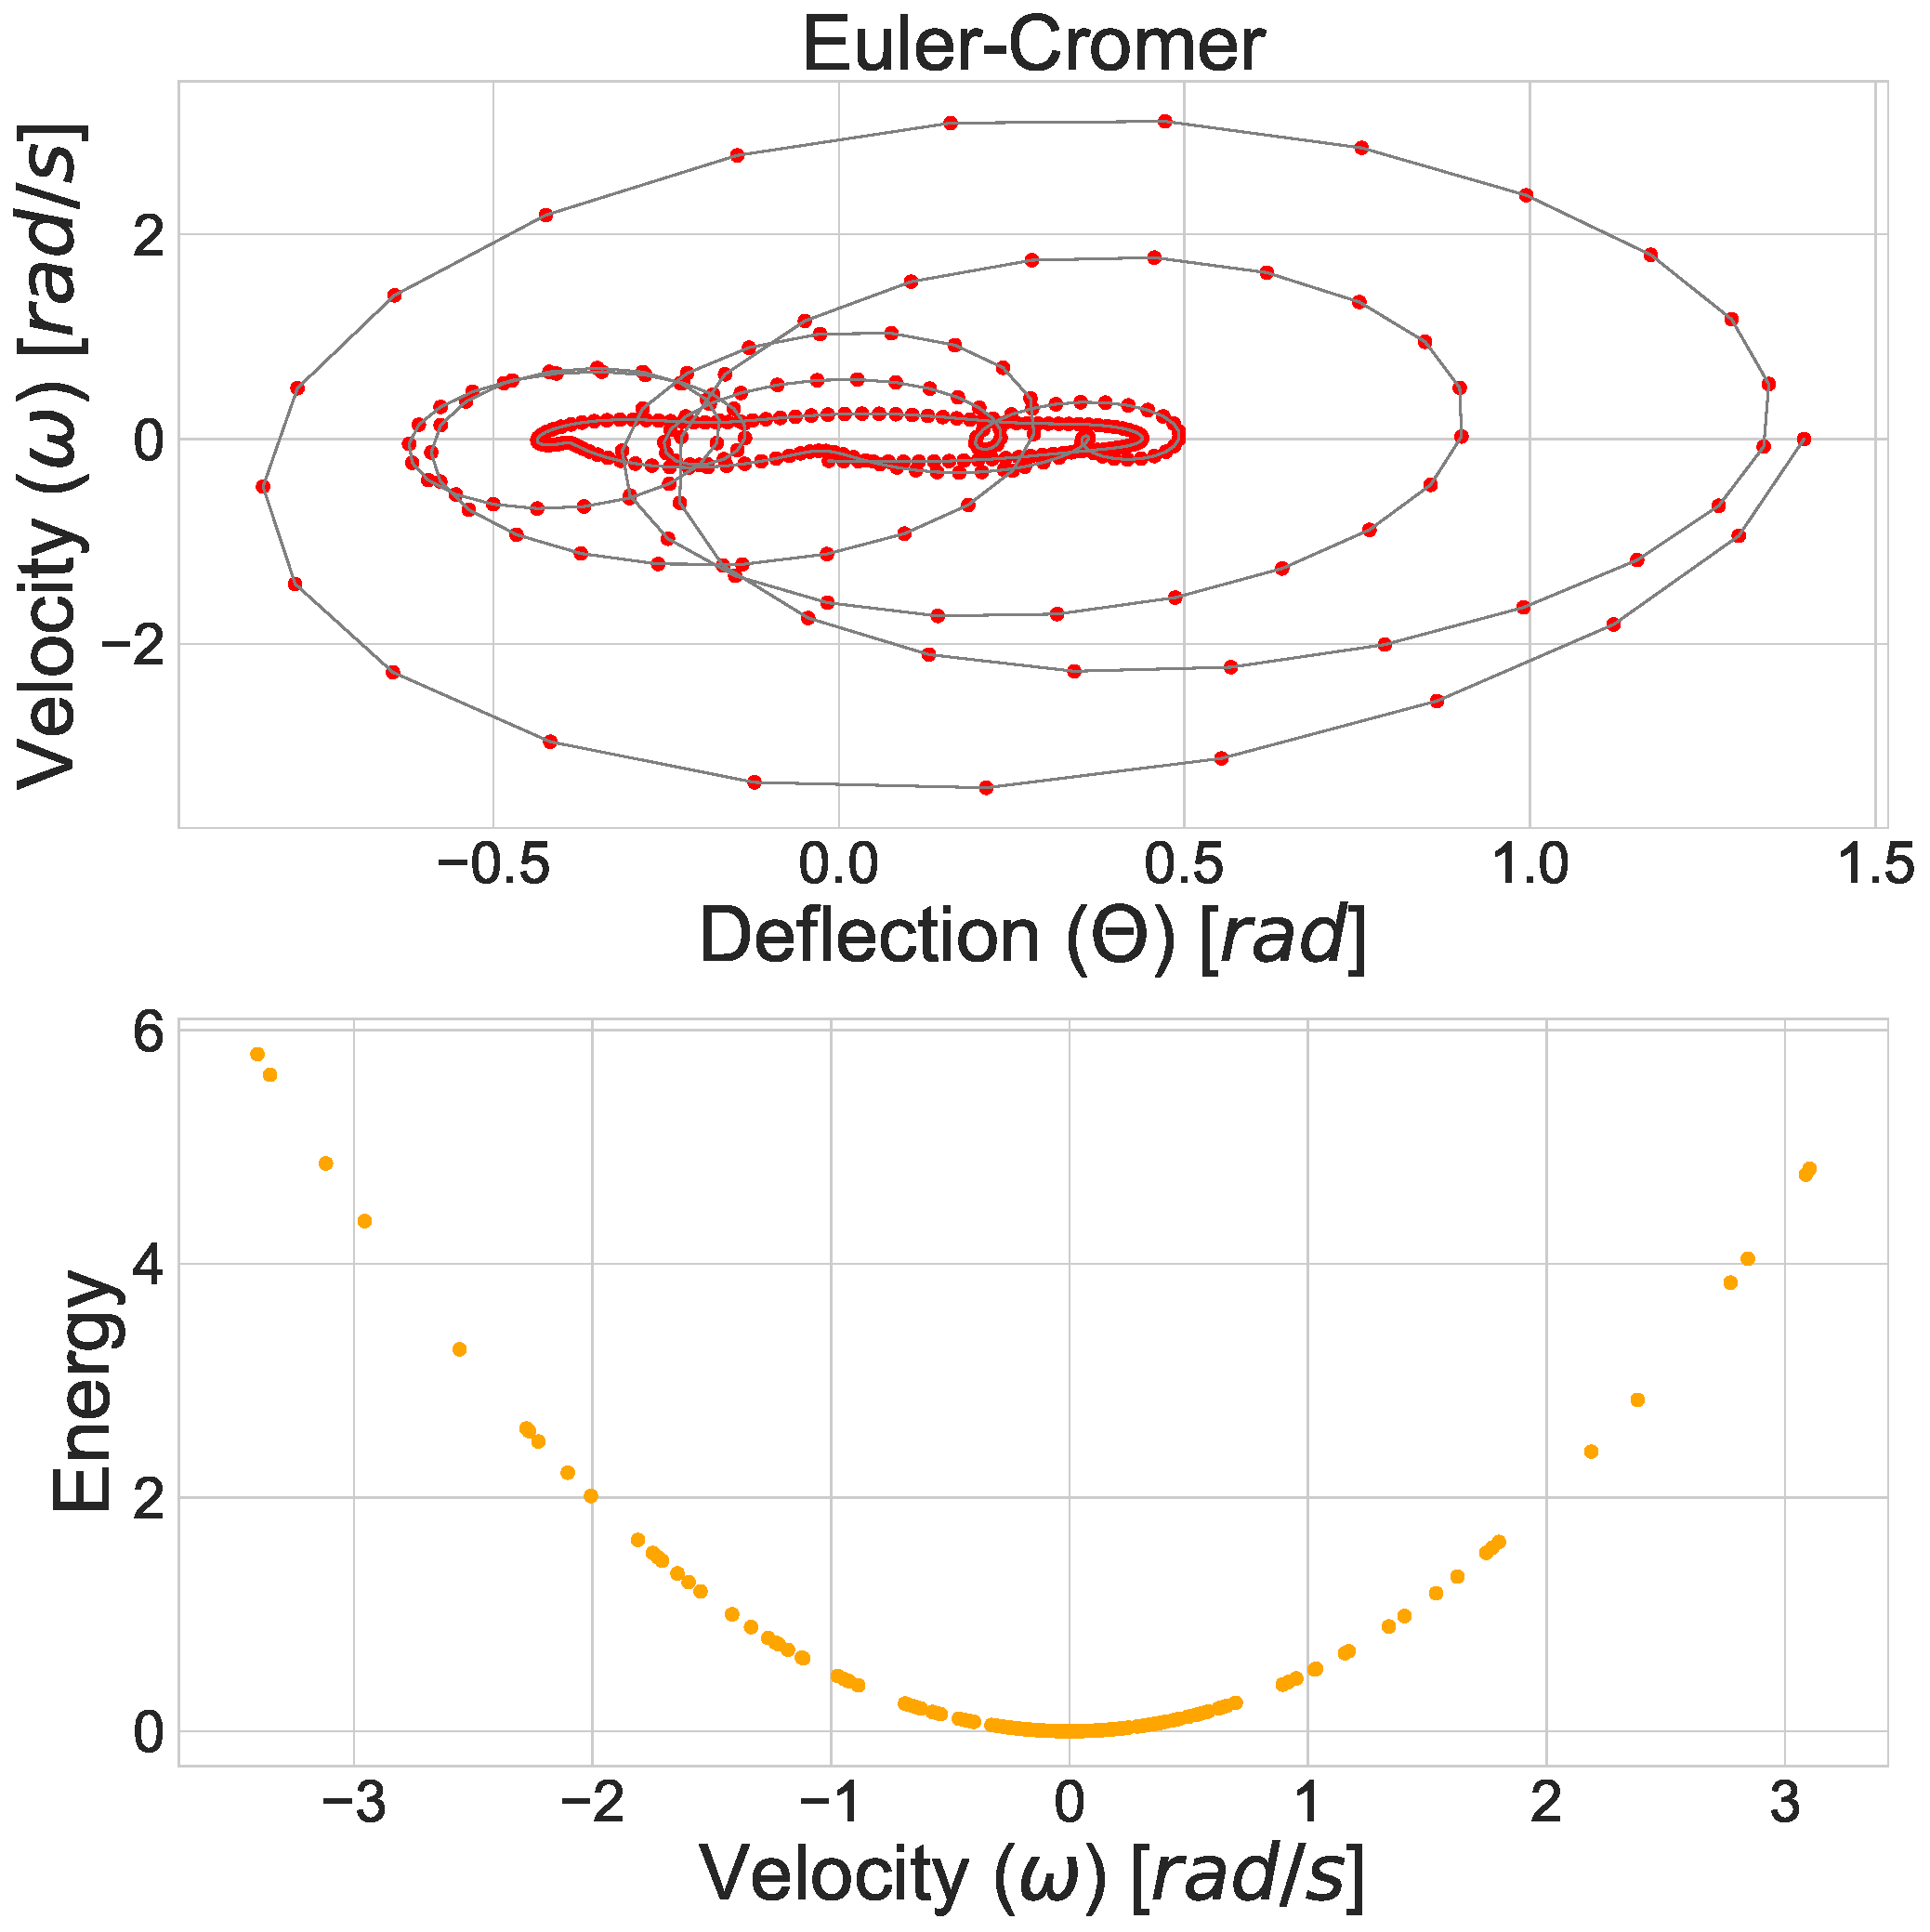
\includegraphics[width=.25\textwidth]{images/phase_energy_eulercromer_dampeddriven.pdf}}
\captionof{figure}{Euler-Cromer\\Damp.-Driv.}\label{fig:50}
\hfill
{\centering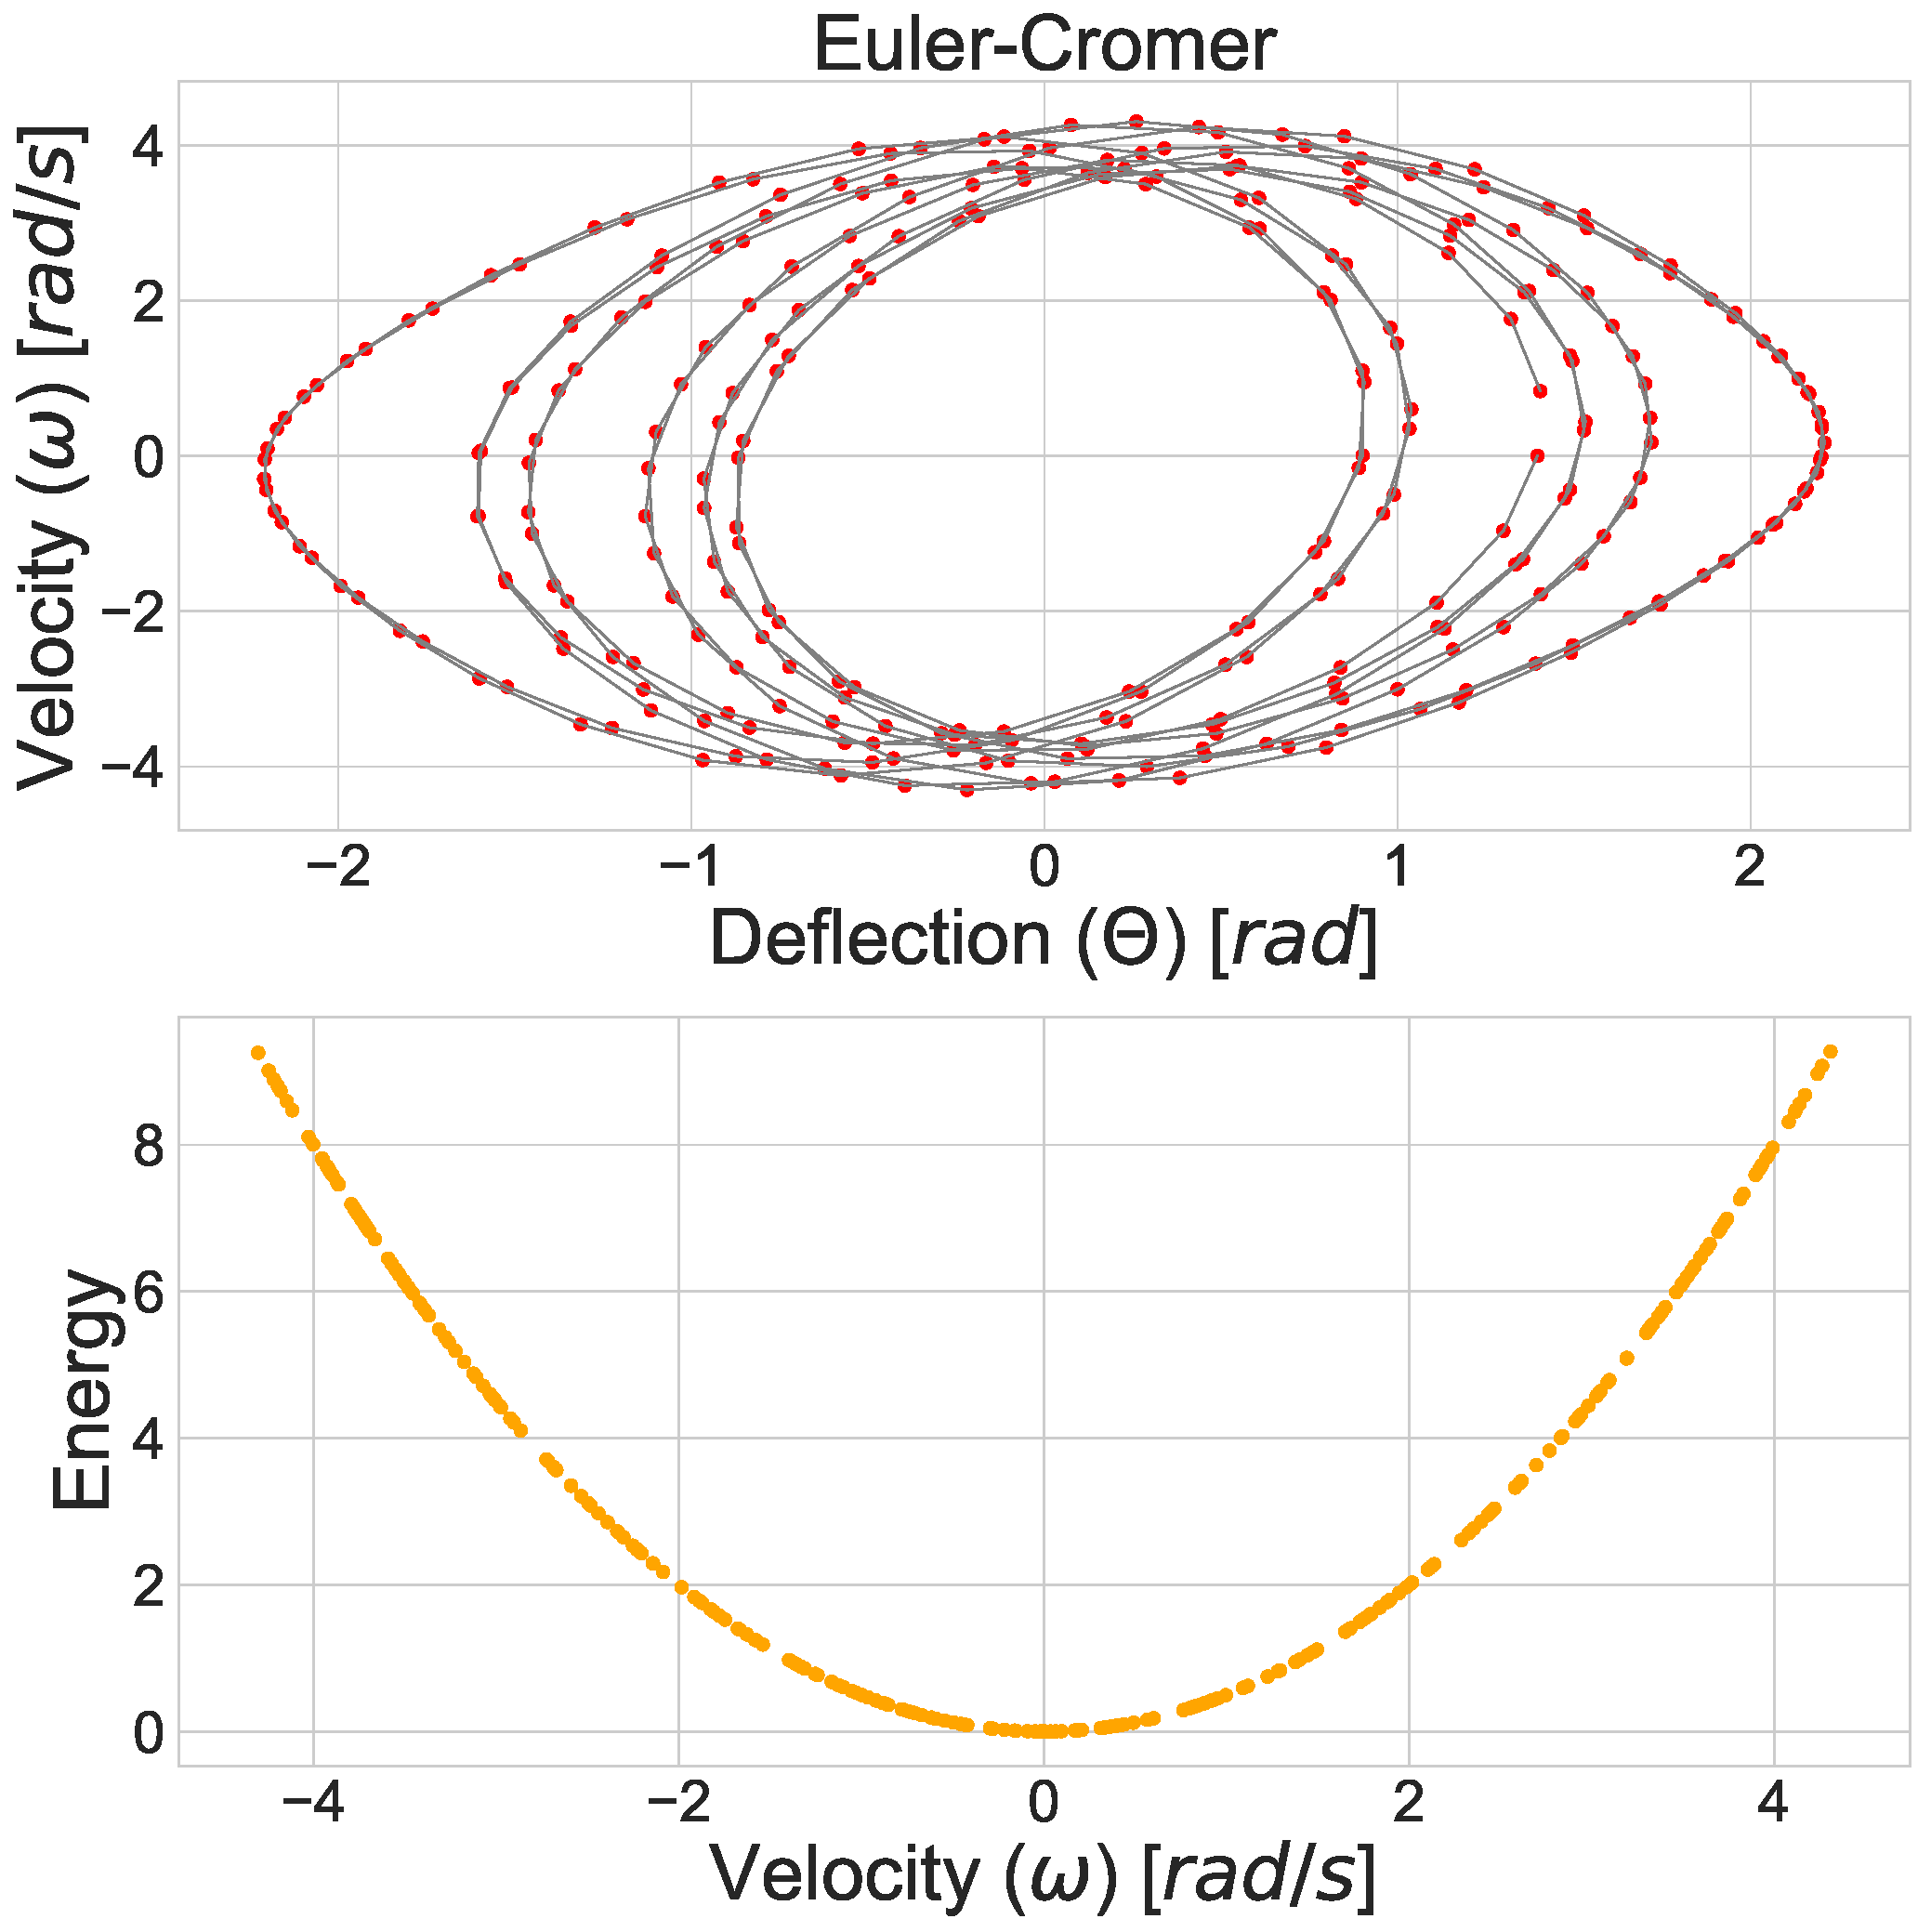
\includegraphics[width=.25\textwidth]{images/phase_energy_eulercromer_driven.pdf}}
\captionof{figure}{Euler-Cromer\\Driv.}\label{fig:51}
\hfill

\end{multicols}

\newpage

\subsubsection*{B.3.\ \ Kitérés-idő és sebesség-idő diagramok diagramok, dupla inga}

\begin{multicols}{4}
{\centering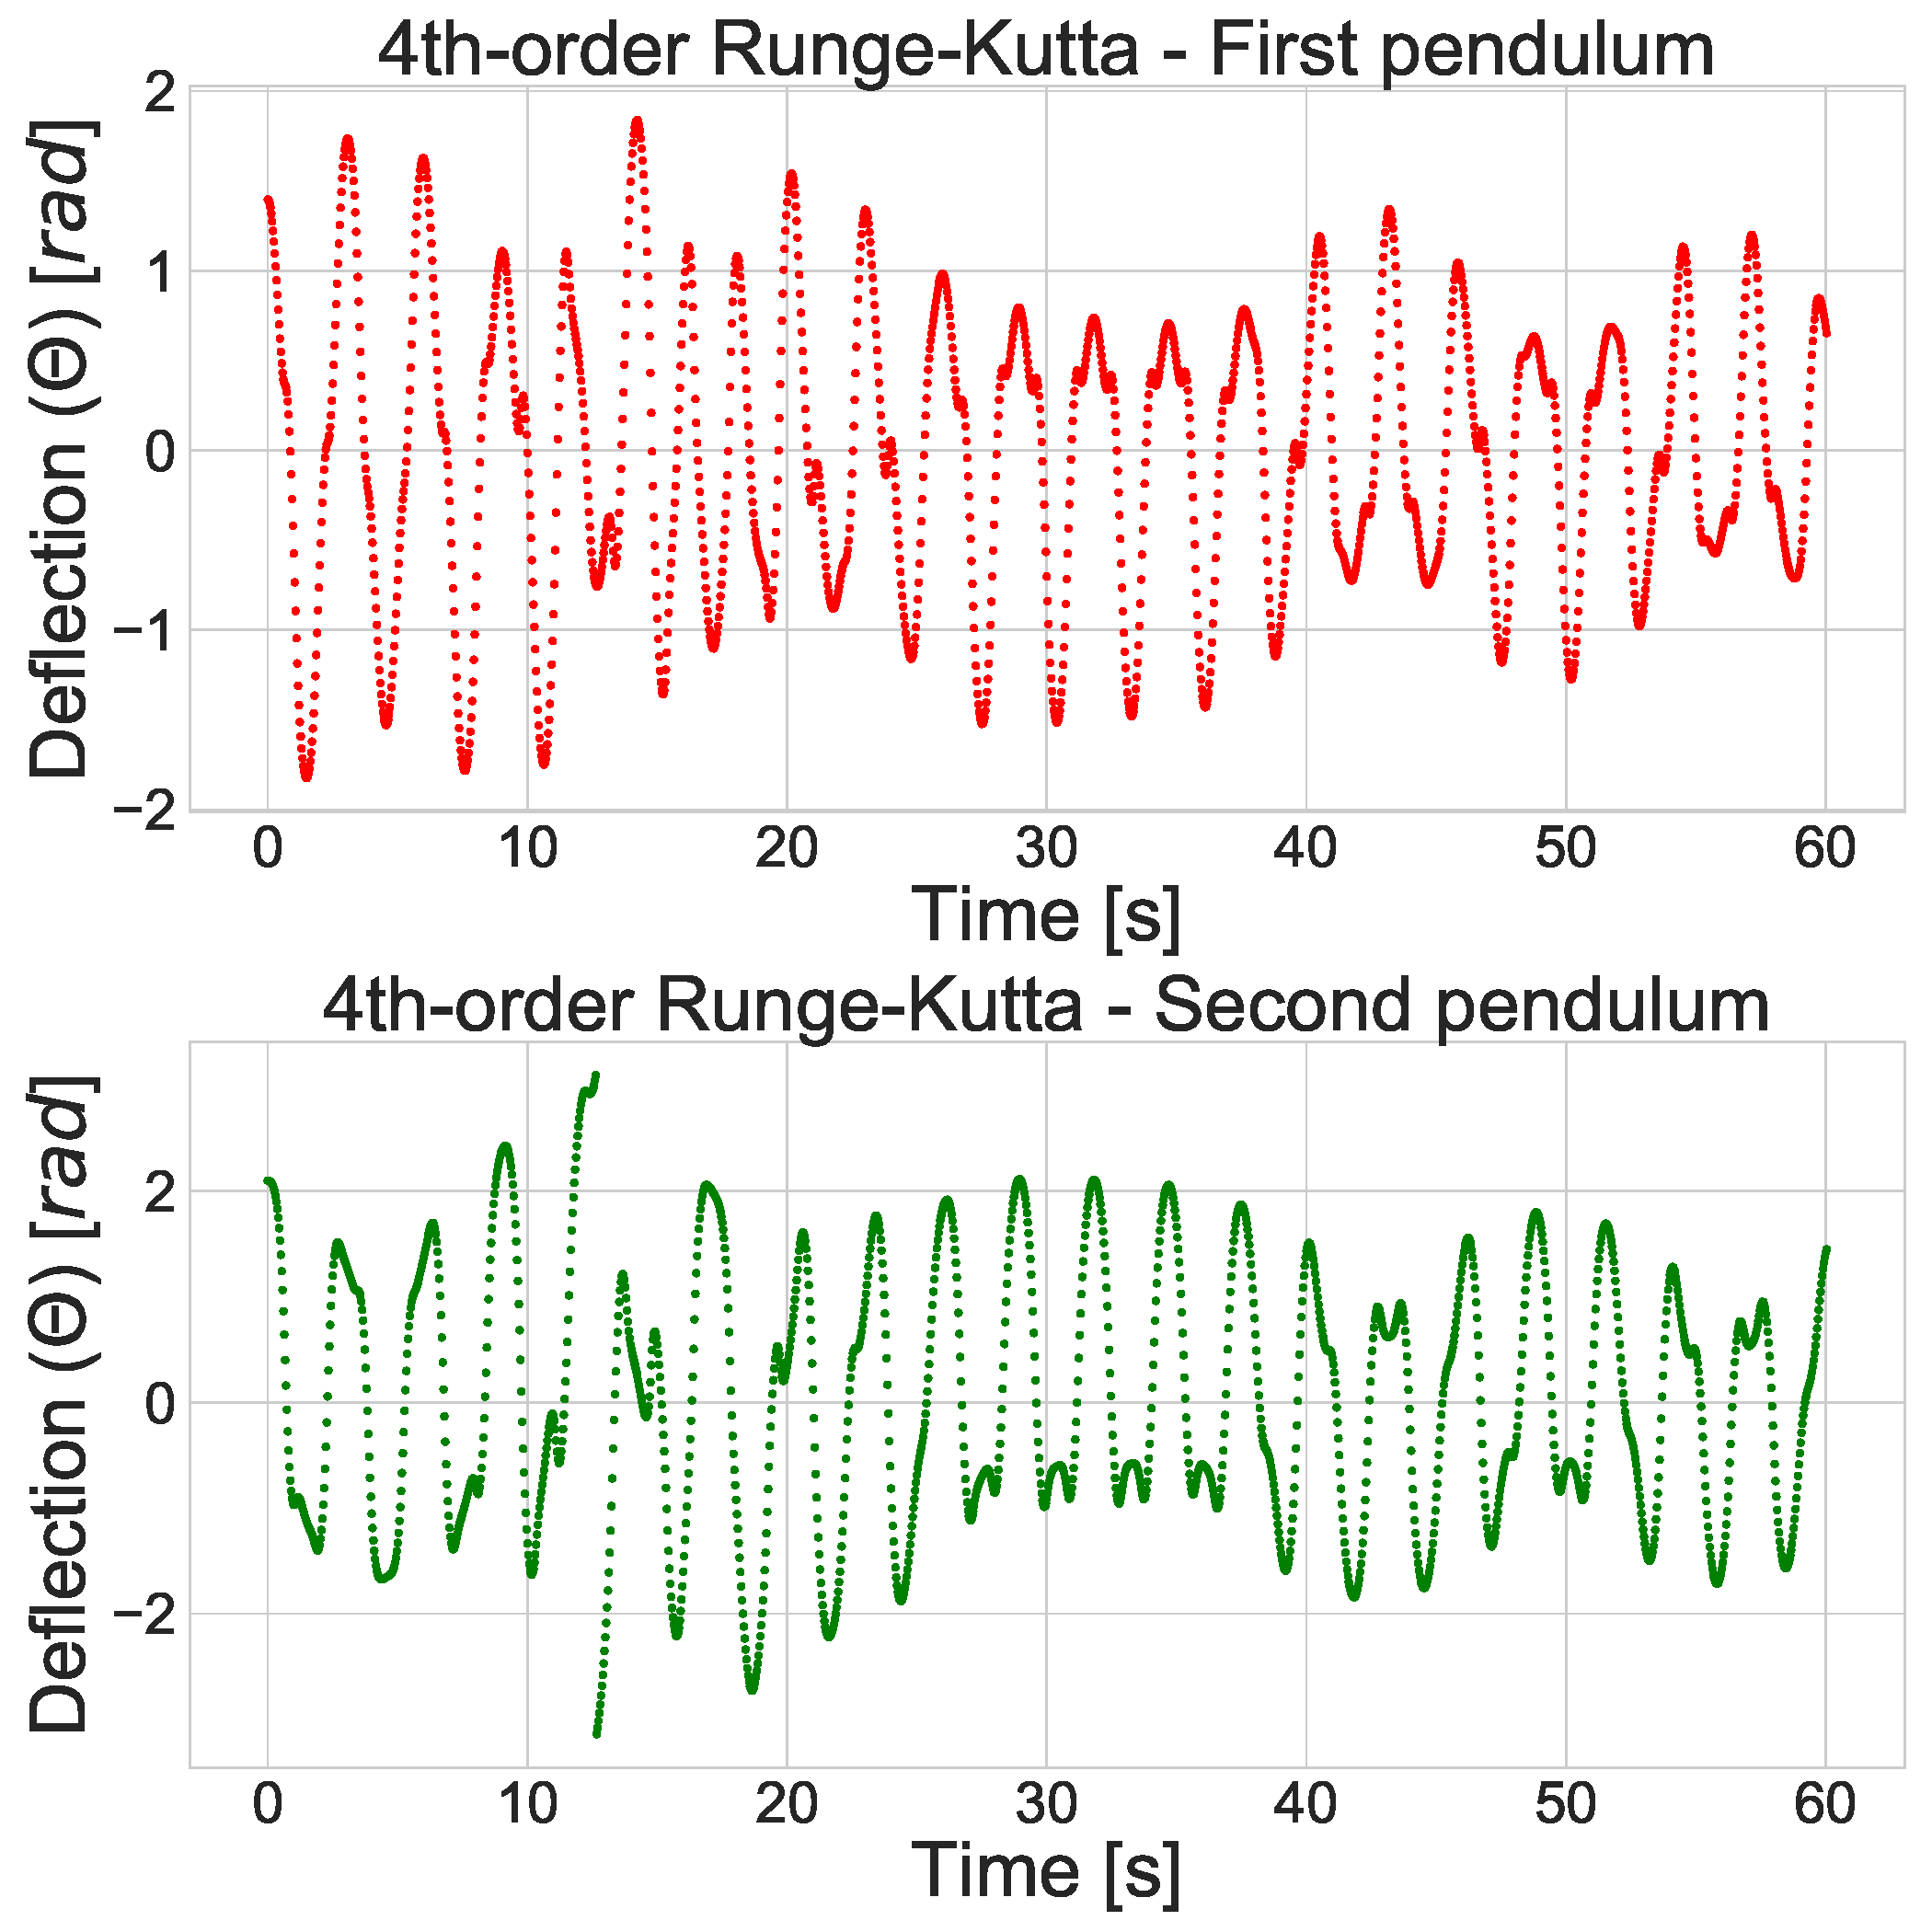
\includegraphics[width=.25\textwidth]{images/theta_omega_runge_double.pdf}}
\captionof{figure}{Runge-Kutta\\Mat.}\label{fig:52}
\hfill
{\centering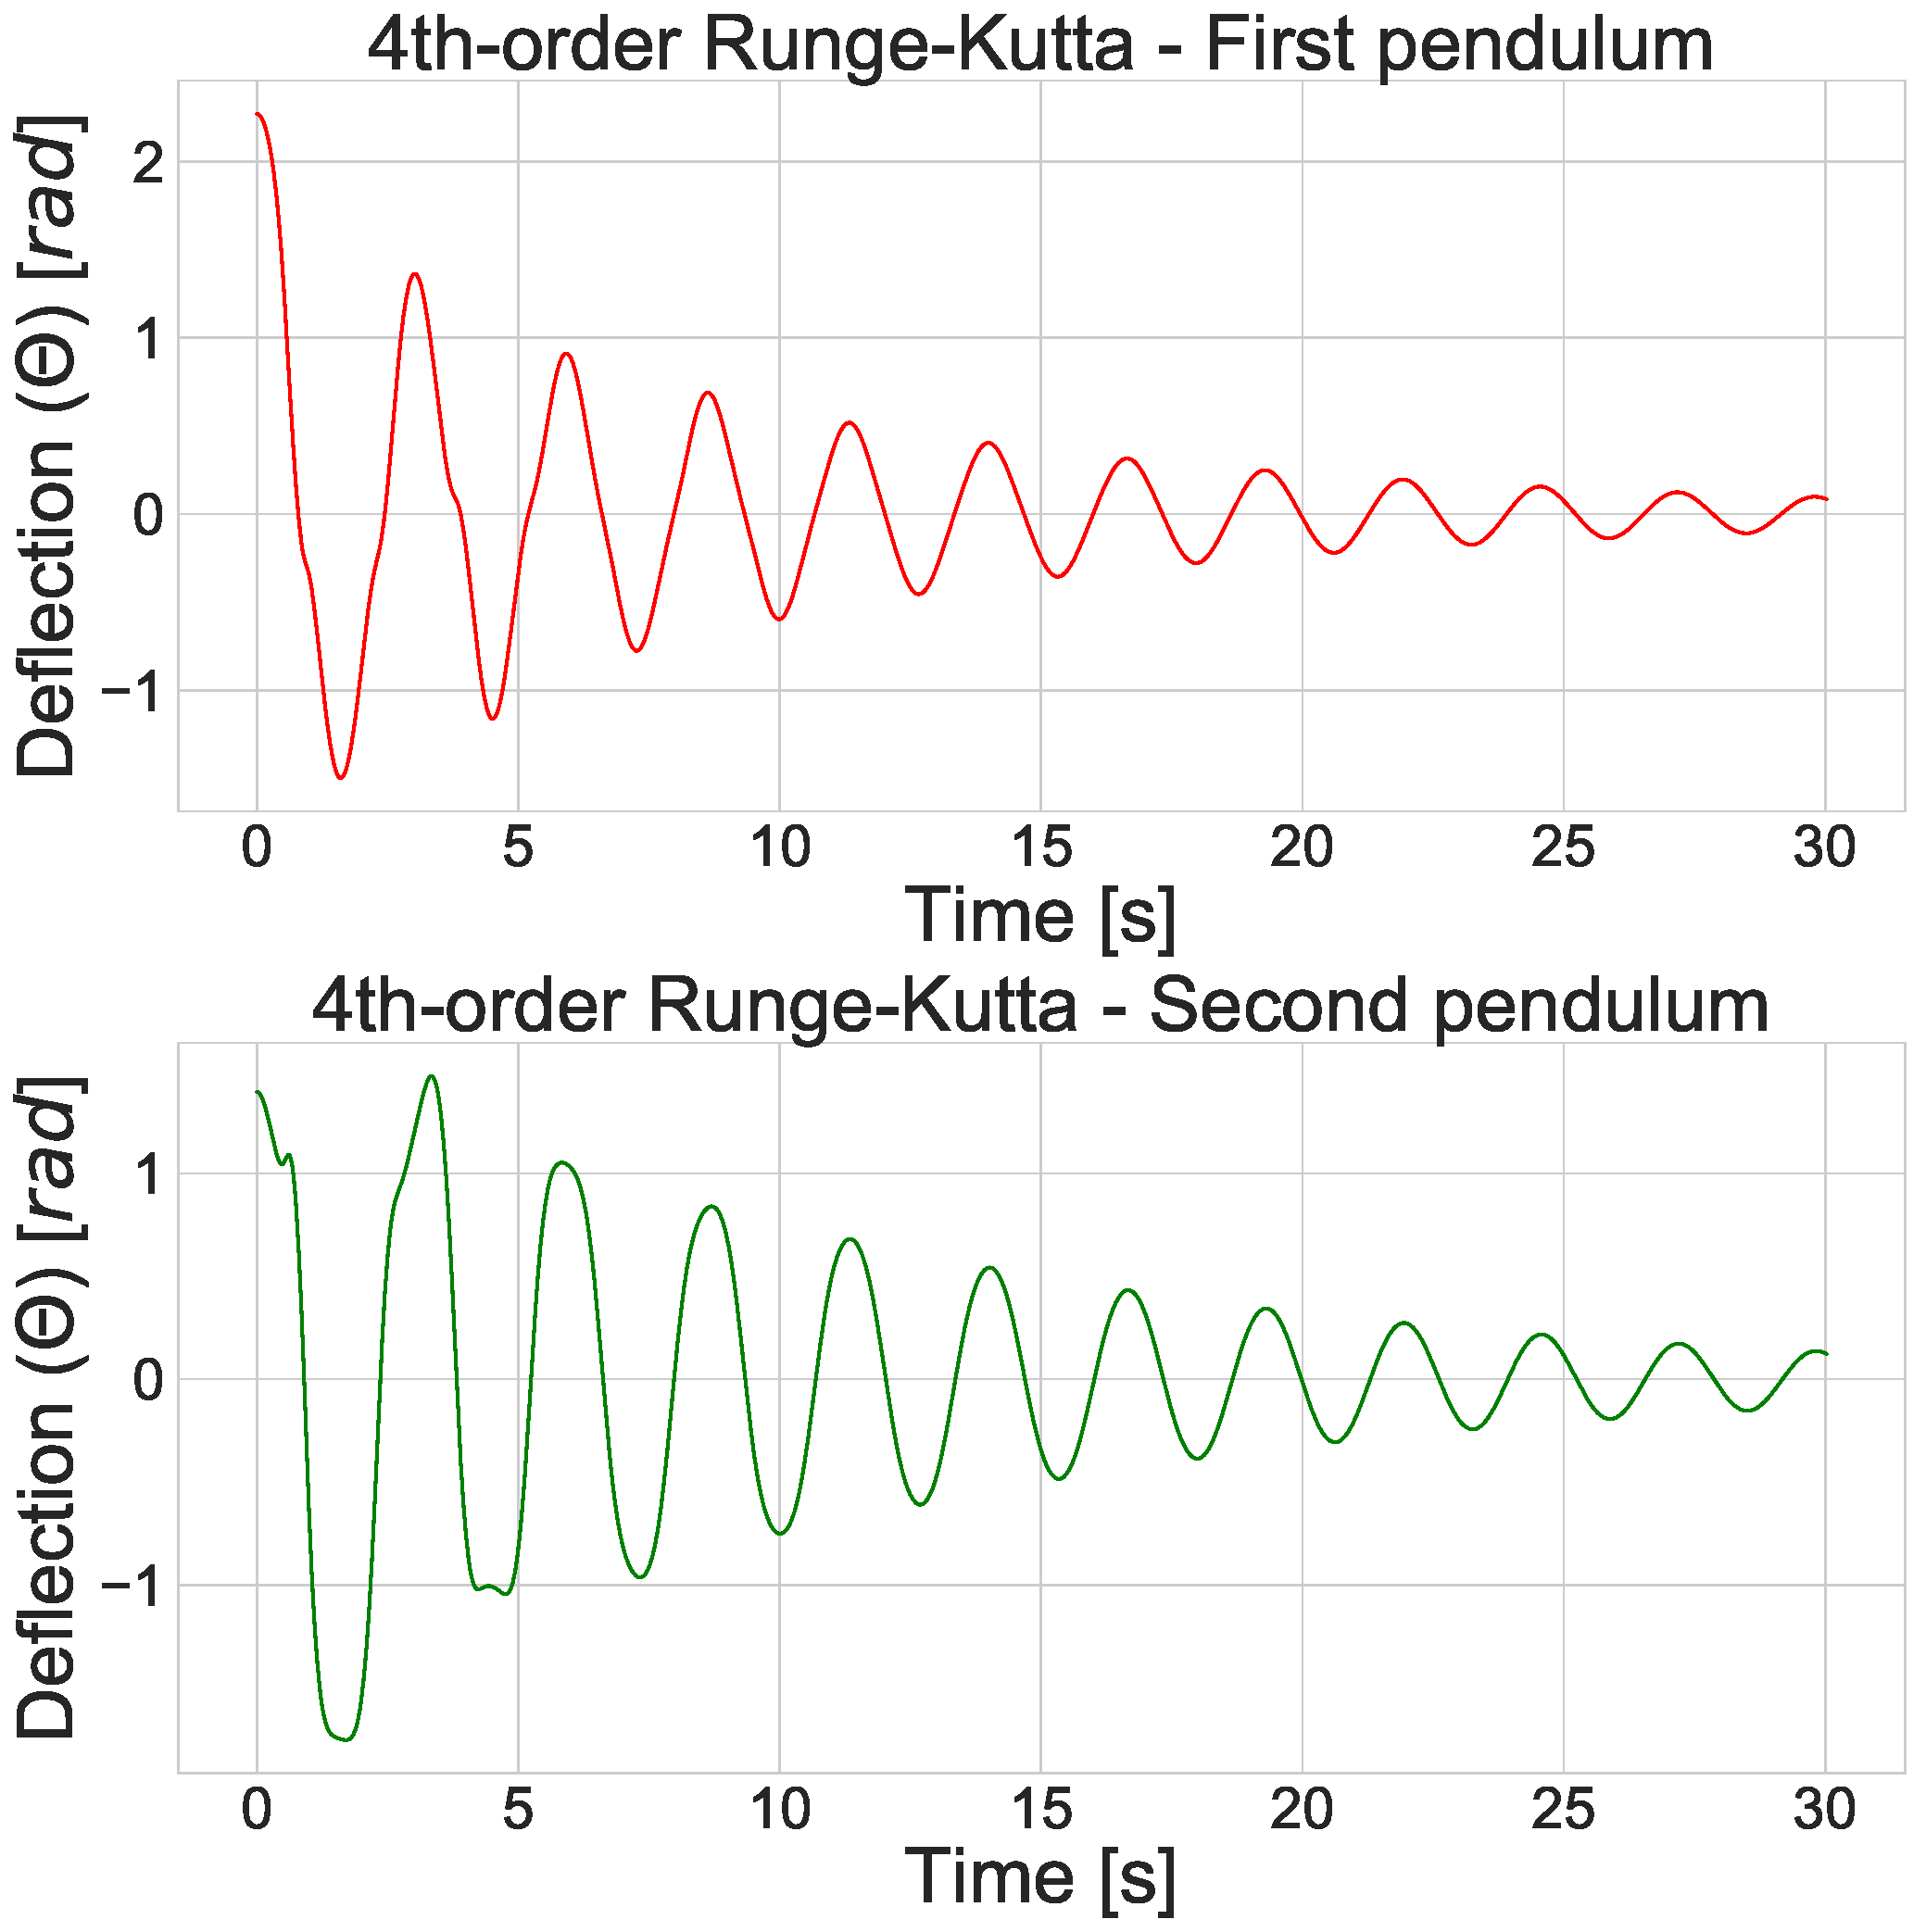
\includegraphics[width=.25\textwidth]{images/theta_omega_runge_double_damped.pdf}}
\captionof{figure}{Runge-Kutta\\Damp.}\label{fig:53}
\hfill
{\centering\includegraphics[width=.25\textwidth]{images/theta_omega_runge_double_dampeddriven.pdf}}
\captionof{figure}{Runge-Kutta\\Damp.-Driv.}\label{fig:54}
\hfill
{\centering\includegraphics[width=.25\textwidth]{images/theta_omega_runge_double_driven.pdf}}
\captionof{figure}{Runge-Kutta\\Driv.}\label{fig:55}
\hfill

\end{multicols}
\begin{multicols}{4}

{\centering\includegraphics[width=.25\textwidth]{images/theta_omega_rkck_double.pdf}}
\captionof{figure}{R-K-C-K\\Mat.}\label{fig:56}
\hfill
{\centering\includegraphics[width=.25\textwidth]{images/theta_omega_rkck_double_damped.pdf}}
\captionof{figure}{R-K-C-K\\Damp.}\label{fig:57}
\hfill
{\centering\includegraphics[width=.25\textwidth]{images/theta_omega_rkck_double_dampeddriven.pdf}}
\captionof{figure}{R-K-C-K\\Damp.-Driv.}\label{fig:58}
\hfill
{\centering\includegraphics[width=.25\textwidth]{images/theta_omega_rkck_double_driven.pdf}}
\captionof{figure}{R-K-C-K\\Driv.}\label{fig:59}
\hfill

\end{multicols}
\begin{multicols}{4}

{\centering\includegraphics[width=.25\textwidth]{images/compare_rk4_rkck_theta_omega.pdf}}
\captionof{figure}{Comparsion\\Mat.}\label{fig:60}
\hfill
{\centering\includegraphics[width=.25\textwidth]{images/compare_rk4_rkck_theta_omega_damped.pdf}}
\captionof{figure}{Comparsion\\Damp.}\label{fig:61}
\hfill
{\centering\includegraphics[width=.25\textwidth]{images/compare_rk4_rkck_theta_omega_dampeddriven.pdf}}
\captionof{figure}{Comparsion\\Damp.-Driv.}\label{fig:62}
\hfill
{\centering\includegraphics[width=.25\textwidth]{images/compare_rk4_rkck_theta_omega_driven.pdf}}
\captionof{figure}{Comparsion\\Driv.}\label{fig:63}
\hfill

\end{multicols}

\newpage

\subsubsection*{B.4.\ \ Fázistér és energia-sebesség diagramok, dupla inga}

\begin{multicols}{4}

{\centering\includegraphics[width=.25\textwidth]{images/phase_energy_runge_double_first.pdf}}
\captionof{figure}{Runge-Kutta\\First P., Mat.}\label{fig:64}
\hfill
{\centering\includegraphics[width=.25\textwidth]{images/phase_energy_runge_double_first_damped.pdf}}
\captionof{figure}{Runge-Kutta\\First P., Damp.}\label{fig:65}
\hfill
{\centering\includegraphics[width=.25\textwidth]{images/phase_energy_runge_double_first_dampeddriven.pdf}}
\captionof{figure}{Runge-Kutta\\First P., Damp.-Driv.}\label{fig:66}
\hfill
{\centering\includegraphics[width=.25\textwidth]{images/phase_energy_runge_double_first_driven.pdf}}
\captionof{figure}{Runge-Kutta\\First P., Driv.}\label{fig:67}
\hfill

\end{multicols}
\begin{multicols}{4}

{\centering\includegraphics[width=.25\textwidth]{images/phase_energy_runge_double_second.pdf}}
\captionof{figure}{Runge-Kutta\\Second P., Mat.}\label{fig:68}
\hfill
{\centering\includegraphics[width=.25\textwidth]{images/phase_energy_runge_double_second_damped.pdf}}
\captionof{figure}{Runge-Kutta\\Second P., Damp.}\label{fig:69}
\hfill
{\centering\includegraphics[width=.25\textwidth]{images/phase_energy_runge_double_second_dampeddriven.pdf}}
\captionof{figure}{Runge-Kutta\\Second P., Damp.-Driv.}\label{fig:70}
\hfill
{\centering\includegraphics[width=.25\textwidth]{images/phase_energy_runge_double_second_driven.pdf}}
\captionof{figure}{Runge-Kutta\\Second P., Driv.}\label{fig:71}
\hfill

\end{multicols}
\begin{multicols}{4}

{\centering\includegraphics[width=.25\textwidth]{images/phase_energy_rkck_double_first.pdf}}
\captionof{figure}{R-K-C-K\\First P., Mat.}\label{fig:72}
\hfill
{\centering\includegraphics[width=.25\textwidth]{images/phase_energy_rkck_double_first_damped.pdf}}
\captionof{figure}{R-K-C-K\\First P., Damp.}\label{fig:73}
\hfill
{\centering\includegraphics[width=.25\textwidth]{images/phase_energy_rkck_double_first_dampeddriven.pdf}}
\captionof{figure}{R-K-C-K\\First P., Damp.-Driv.}\label{fig:74}
\hfill
{\centering\includegraphics[width=.25\textwidth]{images/phase_energy_rkck_double_first_driven.pdf}}
\captionof{figure}{R-K-C-K\\First P., Driv.}\label{fig:75}
\hfill

\end{multicols}
\begin{multicols}{4}

{\centering\includegraphics[width=.25\textwidth]{images/phase_energy_rkck_double_second.pdf}}
\captionof{figure}{R-K-C-K\\Second P., Mat.}\label{fig:76}
\hfill
{\centering\includegraphics[width=.25\textwidth]{images/phase_energy_rkck_double_second_damped.pdf}}
\captionof{figure}{R-K-C-K\\Second P., Damp.}\label{fig:77}
\hfill
{\centering\includegraphics[width=.25\textwidth]{images/phase_energy_rkck_double_second_dampeddriven.pdf}}
\captionof{figure}{R-K-C-K\\Second P., Damp.-Driv.}\label{fig:78}
\hfill
{\centering\includegraphics[width=.25\textwidth]{images/phase_energy_rkck_double_second_driven.pdf}}
\captionof{figure}{R-K-C-K\\Second P., Driv.}\label{fig:79}
\hfill

\end{multicols}

\newpage

\begin{multicols}{4}

{\centering\includegraphics[width=.25\textwidth]{images/compare_rk4_rkck_phase_energy_first.pdf}}
\captionof{figure}{Comparsion\\Mat.}\label{fig:80}
\hfill
{\centering\includegraphics[width=.25\textwidth]{images/compare_rk4_rkck_phase_energy_first_damped.pdf}}
\captionof{figure}{Comparsion\\Damp.}\label{fig:81}
\hfill
{\centering\includegraphics[width=.25\textwidth]{images/compare_rk4_rkck_phase_energy_first_dampeddriven.pdf}}
\captionof{figure}{Comparsion\\Damp.-Driv.}\label{fig:82}
\hfill
{\centering\includegraphics[width=.25\textwidth]{images/compare_rk4_rkck_phase_energy_first_driven.pdf}}
\captionof{figure}{Comparsion\\Driv.}\label{fig:83}
\hfill

\end{multicols}
\begin{multicols}{4}

{\centering\includegraphics[width=.25\textwidth]{images/compare_rk4_rkck_phase_energy_second.pdf}}
\captionof{figure}{Comparsion\\Second P., Mat.}\label{fig:84}
\hfill
{\centering\includegraphics[width=.25\textwidth]{images/compare_rk4_rkck_phase_energy_second_damped.pdf}}
\captionof{figure}{Comparsion\\Second P., Damp.}\label{fig:85}
\hfill
{\centering\includegraphics[width=.25\textwidth]{images/compare_rk4_rkck_phase_energy_second_dampeddriven.pdf}}
\captionof{figure}{Comparsion\\Second P., Damp.-Driv.}\label{fig:86}
\hfill
{\centering\includegraphics[width=.25\textwidth]{images/compare_rk4_rkck_phase_energy_second_driven.pdf}}
\captionof{figure}{Comparsion\\Second P., Driv.}\label{fig:87}
\hfill

\end{multicols}

\subsubsection*{B.5.\ \ Trajektóriák, dupla inga}

\begin{multicols}{4}

{\centering\includegraphics[width=.25\textwidth]{images/trajectory_runge_double.pdf}}
\captionof{figure}{Runge-Kutta\\Mat.}\label{fig:88}
\hfill
{\centering\includegraphics[width=.25\textwidth]{images/trajectory_runge_double_damped.pdf}}
\captionof{figure}{Runge-Kutta\\Damp.}\label{fig:89}
\hfill
{\centering\includegraphics[width=.25\textwidth]{images/trajectory_runge_double_dampeddriven.pdf}}
\captionof{figure}{Runge-Kutta\\Damp.-Driv.}\label{fig:90}
\hfill
{\centering\includegraphics[width=.25\textwidth]{images/trajectory_runge_double_driven.pdf}}
\captionof{figure}{Runge-Kutta\\Driv.}\label{fig:91}
\hfill

\end{multicols}

\begin{multicols}{4}

{\centering\includegraphics[width=.25\textwidth]{images/trajectory_rkck_double.pdf}}
\captionof{figure}{R-K-C-K\\Mat.}\label{fig:92}
\hfill
{\centering\includegraphics[width=.25\textwidth]{images/trajectory_rkck_double_damped.pdf}}
\captionof{figure}{R-K-C-K\\Damp.}\label{fig:93}
\hfill
{\centering\includegraphics[width=.25\textwidth]{images/trajectory_rkck_double_dampeddriven.pdf}}
\captionof{figure}{R-K-C-K\\Damp.-Driv.}\label{fig:94}
\hfill
{\centering\includegraphics[width=.25\textwidth]{images/trajectory_rkck_double_driven.pdf}}
\captionof{figure}{R-K-C-K\\Driv.}\label{fig:95}
\hfill

\end{multicols}

\newpage

\subsubsection*{B.6.\ \ Kaotikus viselkedés, dupla inga}

\begin{multicols}{4}

{\centering\includegraphics[width=.25\textwidth]{images/chaotic_runge_double_diff.pdf}}
\captionof{figure}{Runge-Kutta\\Mat.}\label{fig:96}
\hfill
{\centering\includegraphics[width=.25\textwidth]{images/chaotic_runge_double_diff_damped.pdf}}
\captionof{figure}{Runge-Kutta\\Damp.}\label{fig:97}
\hfill
{\centering\includegraphics[width=.25\textwidth]{images/chaotic_runge_double_diff_dampeddriven.pdf}}
\captionof{figure}{Runge-Kutta\\Damp.-Driv.}\label{fig:98}
\hfill
{\centering\includegraphics[width=.25\textwidth]{images/chaotic_runge_double_diff_driven.pdf}}
\captionof{figure}{Runge-Kutta\\Driv.}\label{fig:99}
\hfill

\end{multicols}
\begin{multicols}{4}

{\centering\includegraphics[width=.25\textwidth]{images/chaotic_rkck_double_diff.pdf}}
\captionof{figure}{R-K-C-K\\Mat.}\label{fig:100}
\hfill
{\centering\includegraphics[width=.25\textwidth]{images/chaotic_rkck_double_diff_damped.pdf}}
\captionof{figure}{R-K-C-K\\Damp.}\label{fig:101}
\hfill
{\centering\includegraphics[width=.25\textwidth]{images/chaotic_rkck_double_diff_dampeddriven.pdf}}
\captionof{figure}{R-K-C-K\\Damp.-Driv.}\label{fig:102}
\hfill
{\centering\includegraphics[width=.25\textwidth]{images/chaotic_rkck_double_diff_driven.pdf}}
\captionof{figure}{R-K-C-K\\Driv.}\label{fig:103}
\hfill

\end{multicols}